%%=============================================================================
%% main.tex — 성균관대학교 박사학위논문(영문) — 본심사판 (2026-09)
%%   An Automated 3D Mapping and Point Cloud Semantic Modeling Framework
%%   for Spatial-Operation Robots — Sangmin Kim
%%
%%  컴파일(반드시 XeLaTeX + BibTeX):
%%    xelatex main ; bibtex main ; xelatex main ; xelatex main
%%    또는: latexmk -xelatex main.tex
%%=============================================================================
\documentclass[11pt,a4paper]{skkuthesis}
\usepackage{url}
\setkeys{Gin}{height=0.82\textheight,keepaspectratio}  % 그림이 한 쪽을 넘지 않도록

%%---- 논문 정보 ----
\dissertationtitle{An Automated 3D Mapping and\\
  Point Cloud Semantic Modeling\\
  Framework for\\
  Spatial-Operation Robots}
\koreantitle{공간 작업 로봇을 위한 자동화된\\3D 매핑 및 포인트클라우드\\시맨틱 모델링 프레임워크}
\authorname{Sangmin Kim}
\koreanauthorname{김 상 민}
\departmentname{Electrical and Computer Engineering}
\koreandepartment{전자전기컴퓨터공학과}
\degreedate{October 2026}        % 표지 / 심사청구서 날짜 (2027년 2월 졸업 — 학과 지침 확인)
\approvaldate{December 2026}     % 인정서(본심사 통과) 날짜 (확정 후 수정)
\advisorname{Taeyong Kuc}        % 지도교수
\spineyear{2027}                 % 측면표지(책등) 연도

%% 심사위원 성명(인정서 서명란 아래 인쇄) — 확정되면 수정
\committeechair{}
\committeeone{}
\committeetwo{}
\committeethree{}

\begin{document}

%%====================== 1. 표지류 ==============================
\makecover
\makeinsidecover
\makesubmission
\makeapproval

%%====================== 2. 앞부분 =================
\frontmatterstyle

\tableofcontents
\listoftables
\listoffigures

\begin{englishabstract}
Three-dimensional (3D) mapping and semantic modeling have become foundational
capabilities for autonomous robots. As the environments in which robots operate
grow more complex and extend vertically, the quality of the underlying 3D
representation determines the range of operations a robot can perform. A
well-constructed 3D semantic model captures the geometry of a space, the
identity and attributes of its objects, and the relationships among them, so
that heterogeneous downstream robots can share one understanding of the
environment. Two gaps persist in current practice. First, survey-grade
terrestrial laser scanners (TLS) deliver millimeter-accurate geometry but
require minutes of stationary acquisition per pose and register scans only
offline, so conventional exploration algorithms that assume continuous motion
and online registration cannot drive them. Second, semantic information is
usually produced as auxiliary annotation rather than as a verified, queryable,
and maintainable knowledge representation, and open-vocabulary 3D classifiers
that work on curated indoor benchmarks propagate confident but wrong labels on
industrial content.

This dissertation proposes and validates an integrated framework in which a
mobile robot carrying a survey-grade TLS autonomously acquires a 3D map of an
unknown indoor environment, a fully automated pipeline converts the registered
point cloud into a confidence-aware ontological semantic knowledge graph, and
the same graph supplies a digital twin, a management console, and a physical
robot. The framework has three parts. Part~A automates acquisition through a
stop-and-scan-integrated frontier exploration strategy in which the decision to
halt and scan is driven by an occlusion-aware ray-cast visibility coverage
model computed on the live occupancy grid rather than by Euclidean proximity.
In a controlled paired ablation the visibility rule raises line-of-sight (LOS)
coverage from about 77\% to 84--85\% for one to two additional scans, and in a
fully autonomous on-hardware comparison with a Leica BLK360 it raises LOS
coverage from 77.6\% to 92.1\% while every visibility run registers offline at
survey grade (4--5\,mm bundle error). Part~B converts the registered scan into
a Triplet Ontological Semantic Model (TOSM) knowledge graph through a
deterministic geometric backbone (seeded structure removal, fixed-parameter
decomposition with a structure-remnant filter, and explicit modeling) followed
by multi-view vision--language-model (VLM) verification with confidence-weighted
late fusion and automatic escalation, identity-preserving incremental updates,
structurally gated querying, an object-grounded place layer, and an
owner-in-the-loop revision path. Escalation lifts verification accuracy from
77.8\% to 88.9\% and from 78.1\% to 84.4\% on two configurations of an
industrial room, with 94--100\% precision on unanimous votes; structural gating
answers 83.3\% of knowledge-grounded questions while blocking hallucination
traps; selective re-verification reduces VLM cost to 3.1\% of a rebuild on a
controlled re-scan; and a real three-epoch study preserves node identities with
zero observed identity switches. Part~C validates the representation downstream:
an automated scan-to-simulation pipeline builds a physics-enabled NVIDIA Isaac
Sim twin in under 80~s that preserves metric scale to within 2\%, a live
bidirectional bridge mirrors the physical mobile manipulator at 30~Hz with 5.5~cm
mean end-to-end positioning error, and console-issued semantic missions are
resolved against the graph and executed by the physical robot with a mean
arrival error of 0.30~m, while owner-refuted phantom goals are refused with
zero motion.

Together, the results establish an end-to-end path from autonomous survey-grade
acquisition, through verified and maintainable semantic modeling, to
consumption by a real spatial-operation robot, and they identify the remaining
limits---3D visibility, vocabulary gaps for site-specific equipment, and
multi-site validation---as the directions for future work.
\keywords{3D Semantic Mapping, Terrestrial Laser Scanning, Stop-and-Scan
Exploration, Visibility Coverage, Vision--Language Model Verification, Triplet
Ontological Semantic Model, Knowledge Graph, Digital Twin}
\end{englishabstract}

%%====================== 3. 본문 ====================
\mainmatterstyle

%%=============================================================================
%% chapters/chapter1.tex — Introduction (final-defense version)
%%=============================================================================
\chapter{Introduction}
\label{ch:intro}

\section{Background and Motivation}
\label{sec:background}

Modern robotic systems are evolving from executing simple, pre-programmed
commands toward intelligent agents that perceive their surroundings, reason
about them, and provide services grounded in knowledge of their environment. A
central enabler of this transition is the three-dimensional (3D) representation
of the operating environment. Whereas early mobile robots operated on
two-dimensional (2D) occupancy grids sufficient for collision-free navigation on
a single plane, an increasing number of robotic tasks now extend into the
vertical dimension: a mobile manipulator must reason about the 3D pose of a
graspable object, an industrial lift must localize a ceiling-mounted
installation target, and an inspection robot must relate components distributed
across the full height of a facility. In such settings, the quality of the
underlying 3D representation directly bounds the range of operations a robot
can perform.

A purely geometric point cloud tells a robot where surfaces are, but not what
they are or how they relate to one another. To act intelligently, a robot must
additionally understand the identity, attributes, and relationships of the
objects and places that populate the space. This understanding is captured by a
semantic model: a structured representation that augments raw geometry with
meaning. A well-constructed 3D semantic model serves as a shared substrate for
heterogeneous downstream robots, increasingly mediated by a digital twin---a
continuously updated, machine-readable model of the physical environment that
multiple robots and services can consult, reason over, and update.

Constructing such a representation in practice requires progress along two
tightly coupled fronts. The first is 3D mapping: acquiring and registering point
clouds into a globally consistent map with human intervention minimized.
Industrial, plant, and construction sites are increasingly captured with
survey-grade terrestrial laser scanners (TLS) for as-built modeling and facility
management, because such scanners deliver millimeter-accurate, globally
registered geometry. However, a TLS such as the Leica BLK360 must remain
stationary for minutes per pose and does not register scans in real time.
Conventional frontier-based exploration algorithms assume continuous motion and
online registration and are therefore fundamentally incompatible with this
sensing modality; bridging autonomous exploration and stationary survey-grade
scanning is a prerequisite for the automation this dissertation pursues. The
second front is point cloud semantic modeling: transforming the acquired
geometric data into a structured representation that encodes what each element
means and how elements relate. Converting a raw survey-grade point cloud into a
queryable semantic model that robots can act upon still relies largely on manual
annotation.

Two conceptual gaps motivate this dissertation. First, many existing semantic
mapping frameworks are tied to specific sensor modalities, such as RGB-D
cameras, or assume pre-built static inputs, which limits scalability in
environments that change continuously during operation. Second, semantic
information tends to be generated as auxiliary annotation rather than as a
structured knowledge representation, making it difficult for downstream
services to query, reason over, verify, and extend it. Beyond these, three
practical challenges arise at the implementation level. State-of-the-art 3D
segmentation and open-vocabulary classification models exhibit insufficient
accuracy when applied directly to survey-grade industrial point clouds, so that
pipelines that propagate their labels downstream hand the robot confident
fictions. Language interfaces that answer questions about a scene from an
unvalidated label dump hallucinate facts that a robot would act on. Finally,
scene models are typically built once and abandoned: a re-scan either rebuilds
everything, losing the object identities that planners and logs refer to, or is
not integrated at all, even though real sites drift continuously.

\section{Research Objectives}
\label{sec:objectives}

The objective of this dissertation is to propose and validate an integrated
framework in which a survey-grade 3D-point-cloud-laser-based mapping robot
acquires 3D maps of unknown indoor environments with human intervention
minimized, transforms the acquired point clouds into a verified and maintainable
ontological semantic model through a fully automated semantic modeling and
database construction pipeline, and enables downstream robots to determine
spatial operations semantically on the same representation. To this end, the
research pursues five sub-objectives:

\begin{itemize}[leftmargin=2.2em,itemsep=2pt]
  \item (O1) Design a frontier-based autonomous exploration strategy coupled
        with a stop-and-scan sequence, in which the decision to halt and scan
        is made by an occlusion-aware coverage model computed on the live
        occupancy map, so that stationary survey-grade scanners can be driven
        autonomously with as few scans as genuine observation requires.
  \item (O2) Build an object-level 3D recognition backbone that operates
        directly on survey-grade colored point clouds---preprocessing,
        deterministic geometry-aware decomposition, and open-vocabulary
        provisional classification---whose reproducibility underwrites
        verification and change detection.
  \item (O3) Propose a fully automated semantic modeling pipeline that converts
        recognized objects and places into a confidence-aware ontological
        knowledge graph based on the Triplet Ontological Semantic Model (TOSM),
        in which every label is verified by multi-view vision--language-model
        (VLM) inference with automatic escalation, unresolved content is
        retained as explicitly unverified, identities are preserved across
        re-scans, and query answers are structurally gated.
  \item (O4) Derive from the same 3D semantic model the multilayer,
        robot-consumable representation that spatial operations at different
        heights require---a driving layer (occupancy grid and place layer for
        navigation), a manipulation work layer (verified object footprints and
        poses at reach height), and an overhead layer (ceiling-mounted
        structure recognized from the same scan)---together with a
        physics-enabled simulation stage, so that the representation remains
        compatible with conventional 2D-laser-based navigation stacks and
        with simulation-based commissioning.
  \item (O5) Validate the integrated framework through digital-twin integration
        and consumption by a physical spatial-operation robot---a mobile
        manipulator that drives on the driving layer, manipulates at work
        height, and can point its end effector at overhead targets---so that
        the console, the twin, and the robot act on one semantic store.
\end{itemize}

\section{Contributions}
\label{sec:contributions}

To meet these objectives, this dissertation proposes an end-to-end framework
that minimizes human intervention, organized into three parts
(Figure~\ref{fig:overall})---Part~A: 3D mapping with autonomous exploratory
acquisition; Part~B: fully automated point cloud semantic modeling; and Part~C:
digital-twin-based validation. The principal contributions are as follows.

\begin{enumerate}[leftmargin=2.2em,itemsep=2pt]
  \item \textbf{Stop-and-scan-integrated frontier exploration with an
        occlusion-aware visibility coverage model.} Frontier exploration is
        coupled to a stop-and-scan sequencer through a distance gate and a
        coverage-based scan/skip decision. The conventional isotropic-disk
        coverage model, which counts every free cell within sensing range as
        covered---including cells behind walls---is replaced by a ray-cast
        visibility region computed on the live occupancy grid, a line-of-sight
        (LOS) coverage metric over mapped free space, and a marginal-gain
        placement rule with a dual relative/absolute acceptance criterion and
        an optional coverage-completion phase. A controlled paired ablation
        isolates the coverage model as the decisive factor, and a fully
        autonomous on-hardware comparison with a Leica BLK360 on a mobile
        platform reproduces the gain and shows that every visibility run
        registers offline at survey grade (Chapter~\ref{ch:mapping},
        Section~\ref{sec:exp-mapping}).
  \item \textbf{A deterministic geometric backbone for survey-grade point
        clouds.} Seeded structural-plane removal, fixed-parameter density
        clustering with a conservative giant-split, a geometric
        structure-remnant filter for ceiling-soffit phantoms, and
        principal-component-analysis (PCA)-based explicit modeling run fully
        automatically and reproduce every retained
        cluster byte-identically on the same host and across two x86-64 hosts.
        A comparison against closed-set and projection-based learned
        alternatives on an out-of-distribution industrial scan grounds the
        choice (Section~\ref{sec:backbone}, Section~\ref{sec:exp-seg}).
  \item \textbf{Multi-view VLM verification with automatic escalation and
        confidence tiers.} Each object is classified per rendered view under a
        forced answer schema; votes are fused confidence-weighted; split votes
        escalate automatically to a wider view set; and objects that still fail
        to converge remain explicitly unverified. The study shows that the
        obvious all-views-in-one-prompt strategy degrades accuracy on sparse
        point renders, that per-view late fusion is the strongest multi-view
        rule, and that vote unanimity is a 94--100\%-precise gate
        (Section~\ref{sec:verification}, Section~\ref{sec:exp-verify}).
  \item \textbf{A verified, maintainable TOSM knowledge graph with structural
        query gating, identity-preserving incremental update, an
        object-grounded place layer, and owner-in-the-loop revision.} Node
        identities are minted once and carried by two-pass matching; re-scans
        apply confidence-gated node-level upserts with history; the query-time
        view demotes unverified types structurally rather than by instruction;
        places are segmented from the navigation grid and named from verified
        objects only; and the room occupant's refutations, restorations, and
        corrections enter as highest-trust, time-variant evidence. Corrective
        decomposition layers raise automated recall against an owner-audited
        inventory from 28\% to 85\% (Sections~\ref{sec:matching}--\ref{sec:place},
        Sections~\ref{sec:exp-query}--\ref{sec:exp-endtoend}).
  \item \textbf{An automated scan-to-simulation digital twin and end-to-end
        validation on a physical robot.} A registered scan is converted in
        under 80~s into a physics-enabled NVIDIA Isaac Sim stage with a
        collidable wall layer and a dense colored point layer, coupled
        bidirectionally to a real swerve-drive mobile manipulator through a
        ROS~2 bridge with one-shot anchor calibration. The same knowledge
        graph drives a management console, a semantic mission mediator, a
        behavior-tree executor, and the twin; console-issued semantic missions
        are executed by the physical robot, and phantom goals are refused with
        zero motion (Chapter~\ref{ch:validation},
        Sections~\ref{sec:exp-twin}--\ref{sec:exp-missions}).
\end{enumerate}

\begin{figure}[H]
  \centering
  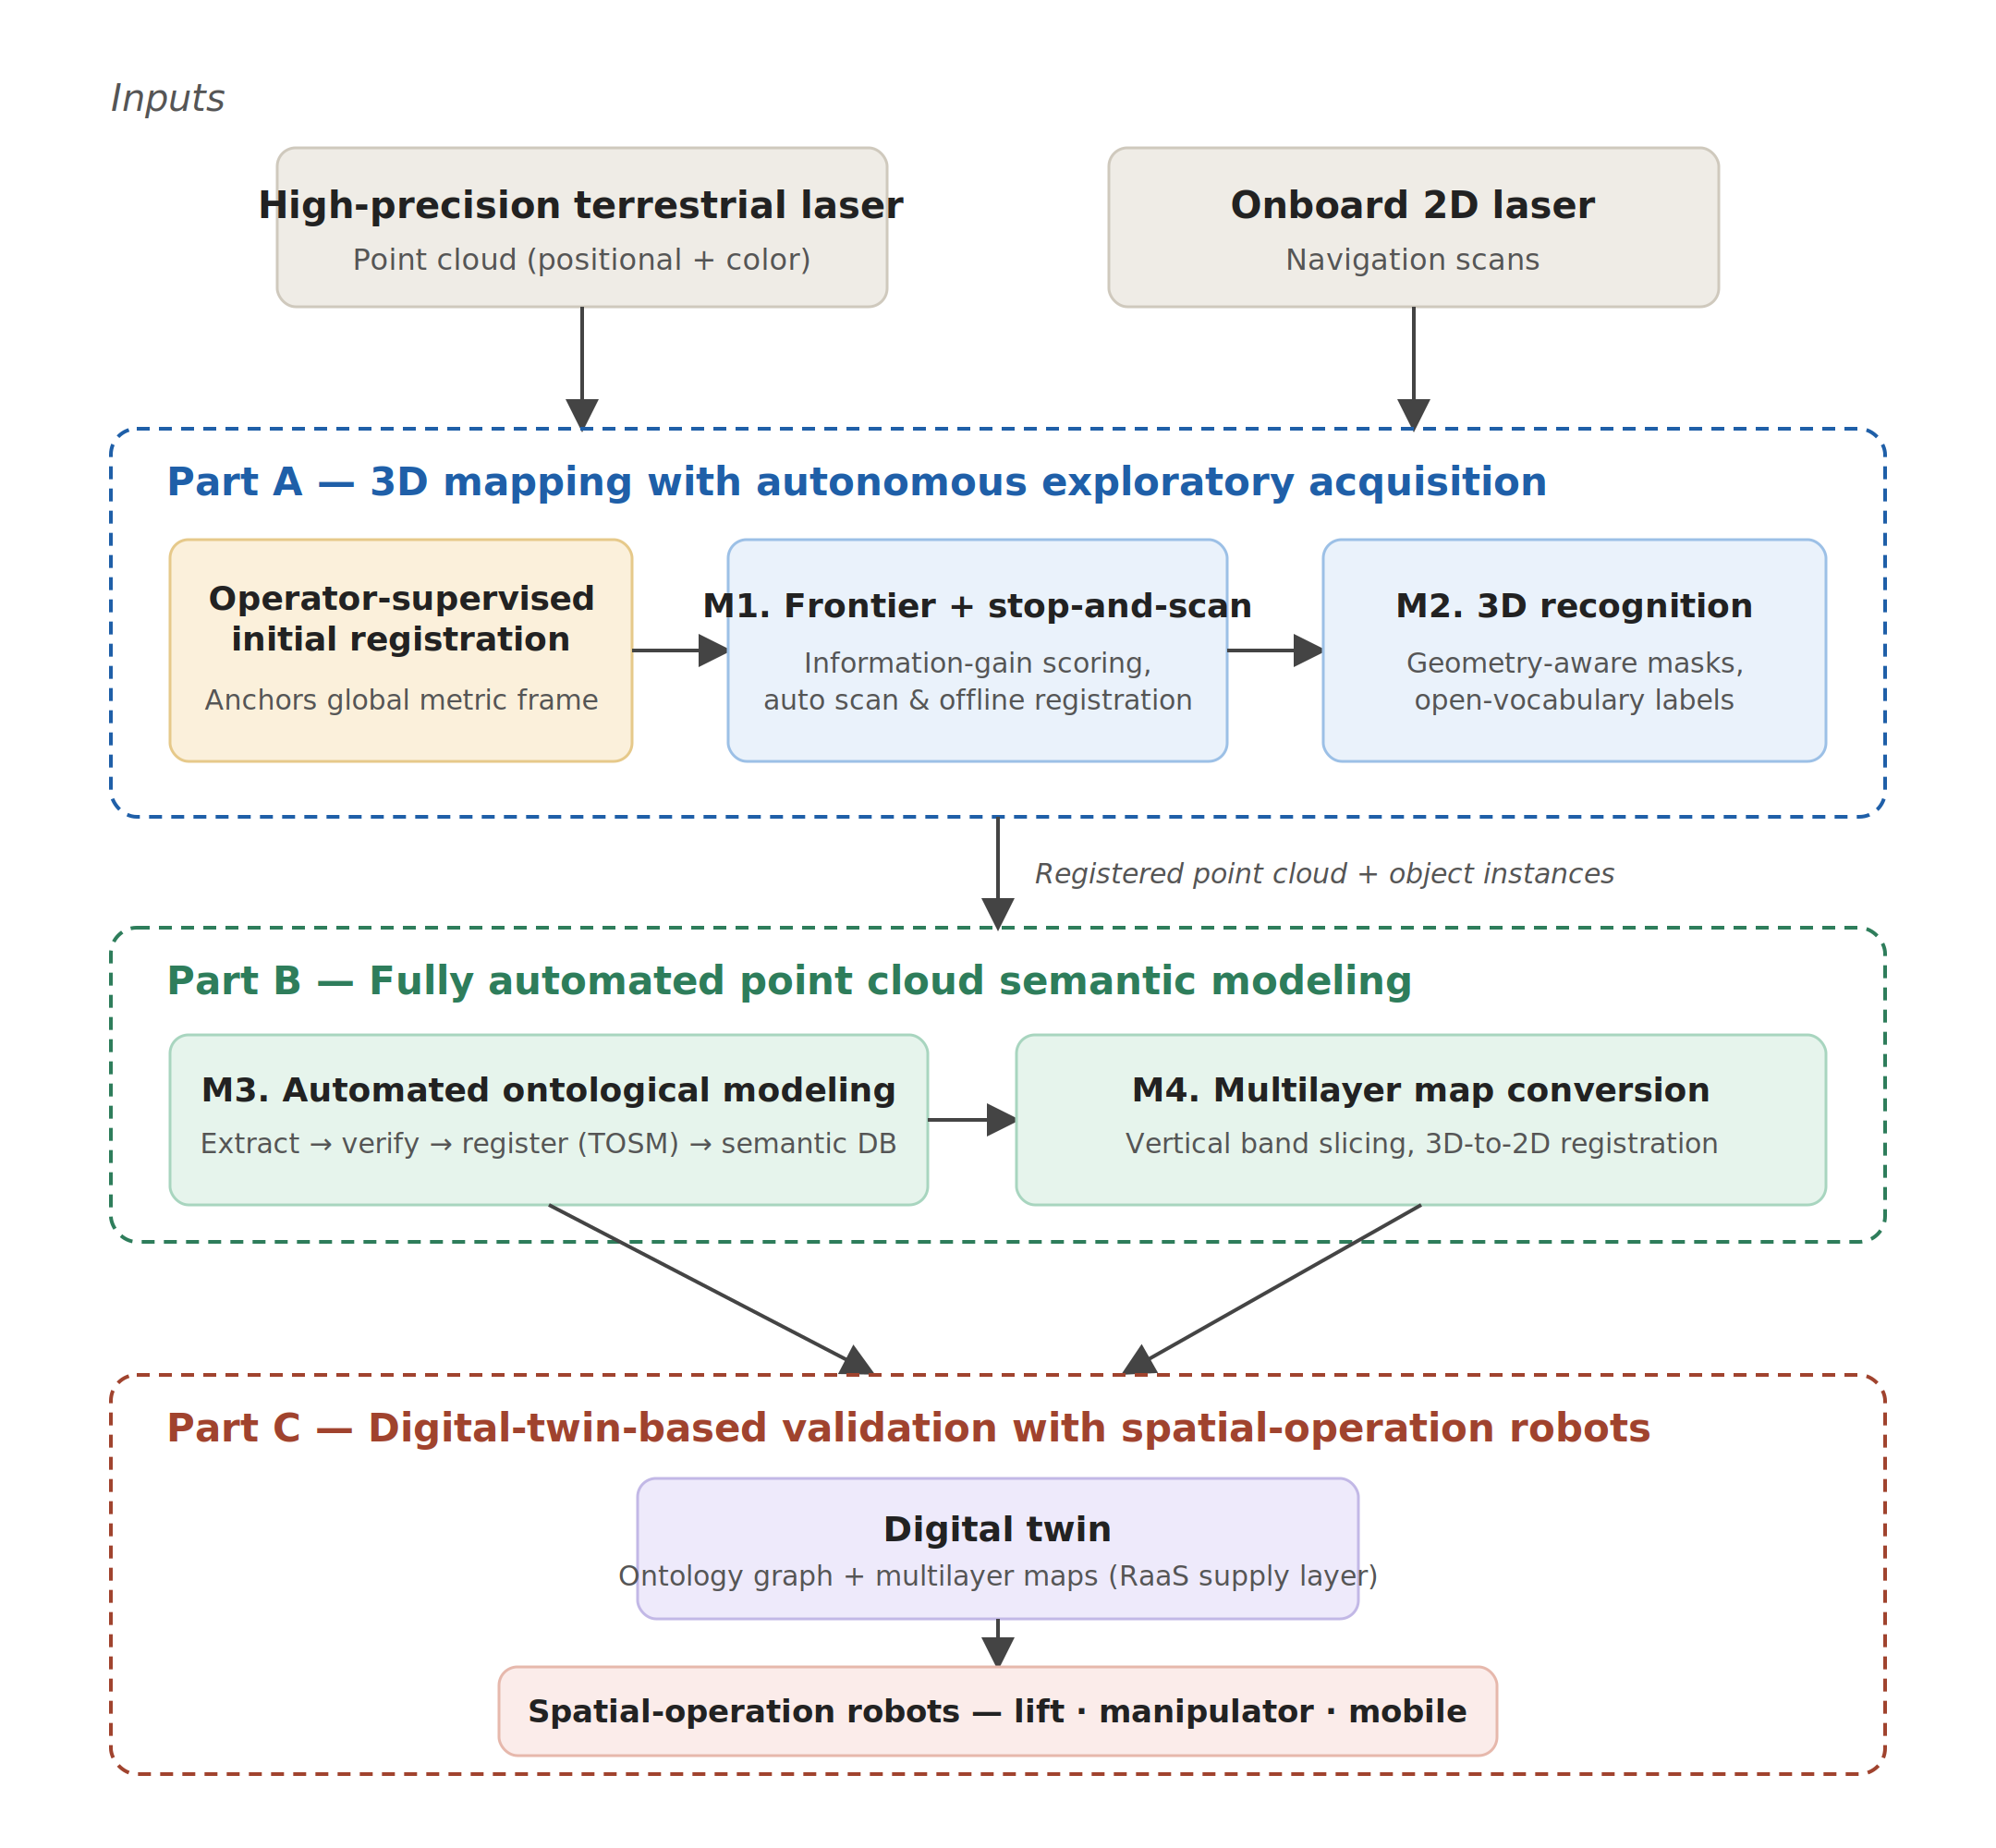
\includegraphics[width=0.95\textwidth]{figures/fig1_1.png}
  \caption{Overall structure of the proposed framework. Part~A performs 3D
  mapping with autonomous exploratory acquisition, Part~B performs fully
  automated point cloud semantic modeling, and Part~C performs
  digital-twin-based validation; a representation generated once by the mapping
  robot is shared and consumed by spatial-operation robots.}
  \label{fig:overall}
\end{figure}

\section{Publications}
\label{sec:publications}

The content of this dissertation has been published, accepted for presentation,
or submitted for publication in the following peer-reviewed venues, all with the author of this dissertation
as first author. Part~A (Chapter~\ref{ch:mapping} and
Section~\ref{sec:exp-mapping}) is based on the coverage-aware stop-and-scan
frontier exploration accepted for presentation at ICCAS~2026~\cite{iccas2026} and its journal
extension with the occlusion-aware visibility coverage model published in
\emph{Sensors}~\cite{kim2026sensors}. Part~B (Chapter~\ref{ch:semantic} and
Sections~\ref{sec:exp-seg}--\ref{sec:exp-ablation}) is based on the multi-view
VLM verification study accepted for presentation at ICTC~2026~\cite{kim2026ictc} and on the
TLS-driven semantic modeling framework (TLS-SMF) submitted to
\emph{Electronics}~\cite{kim2026electronics}. Part~C (Chapter~\ref{ch:validation}
and Sections~\ref{sec:exp-twin}--\ref{sec:exp-missions}) is based on the
automated scan-to-simulation pipeline accepted for presentation at RAAICON~2026~\cite{raaicon2026}
and on the application section of the \emph{Electronics} manuscript. The
knowledge-graph query lineage follows the ISIS~2025 work to which the author
contributed~\cite{kim2025isis}. Where text, tables, or figures are reused from
these publications, the source is indicated at the beginning of the
corresponding chapter.

\section{Dissertation Organization}
\label{sec:organization}

The remainder of this dissertation is organized as follows.
Chapter~\ref{ch:related} reviews related work on autonomous exploration and
coverage models, 3D semantic mapping and open-vocabulary recognition,
VLM-based verification and knowledge-grounded querying, incremental semantic-map
maintenance, and digital twins. Chapter~\ref{ch:mapping} details the automated
3D mapping subsystem: the stop-and-scan frontier exploration architecture, the
visibility-based coverage model, and the placement policy built on it.
Chapter~\ref{ch:semantic} describes the 3D point cloud semantic modeling
subsystem: the deterministic geometric backbone, multi-view VLM verification
with escalation, the TOSM schema and its serialization, identity matching and
confidence-gated update, corrective layers and owner feedback, structurally
gated querying, and the object-grounded place layer.
Chapter~\ref{ch:validation} presents the digital-twin-based validation
architecture: the scan-to-simulation pipeline, the live twin bridge, the
semantic mission stack, and the real-robot integration.
Chapter~\ref{ch:experiments} reports the experimental design and results for
all three parts. Chapter~\ref{ch:conclusion} concludes and discusses future
work.
   % Introduction
%%=============================================================================
%% chapters/chapter2.tex — Related Work (final-defense version)
%%=============================================================================
\chapter{Related Work}
\label{ch:related}

\section{Autonomous Exploration and Next-Best-View Planning}
\label{sec:rw-exploration}

Simultaneous localization and mapping (SLAM) estimates a robot's pose while
reconstructing the geometry of its environment, progressing from filter-based
formulations such as GMapping~\cite{grisetti2007} to graph-based methods such as
Cartographer~\cite{hess2016} that enforce global consistency through loop
closure. Exploration governs how a robot expands its map and reduces
uncertainty, and has been studied principally under two
paradigms~\cite{placed2023,lluvia2021}. Frontier-based methods drive the robot
toward the boundary between known and unknown
space~\cite{yamauchi1997,umari2017}, prioritizing frontiers by expected
information gain and travel cost. Next-best-view (NBV) methods instead evaluate
candidate viewpoints directly by an information-gain or coverage
criterion~\cite{connolly1985,bircher2016}; information-theoretic formulations
make this gain explicit by quantifying the expected reduction in map
uncertainty~\cite{stachniss2005}, and the idea extends to the coordination of
multiple robots~\cite{burgard2005}. Both paradigms have been refined
extensively, for example through improved frontier extraction and cost
shaping~\cite{he2025,quin2021}, incremental frontier structures with
hierarchical planning~\cite{zhou2021}, and sampling-based online informative
path planning~\cite{schmid2020}. Most of these methods, however, assume a
sensor that acquires continuously while the platform moves and registers
incrementally online, so the dominant cost is travel and the act of observing
is effectively free along the path. Under that assumption, the question of
whether to pay a large fixed cost to stop and observe at a particular pose does
not arise. The present work departs from this assumption by introducing a
stop-and-scan exploration strategy whose scan/skip decision is made on the live
map, detailed in Chapter~\ref{ch:mapping}.

\section{Coverage Models, Visibility, and Stop-and-Scan Mapping}
\label{sec:rw-coverage}

The notion that a viewpoint observes only what is in its line of sight is
classical in computational geometry, where the visibility polygon defines the
region directly visible from a point, and in the art-gallery problem, which
asks for a minimal set of guards that jointly see an entire
domain~\cite{gonzalez2002,orourke1987,urrutia2000}. Sensor-coverage and
view-planning formulations build on this idea to place viewpoints that maximize
observed surface, and have been surveyed for automated 3D reconstruction and
inspection~\cite{scott2003}, for sensor planning in computer
vision~\cite{tarabanis1995}, and for view planning in robot active
vision~\cite{zeng2020}. Coverage path planning, which instead seeks a path that
sweeps a sensor footprint over an entire area, has likewise been surveyed
extensively~\cite{choset2001,galceran2013}, including for multi-robot model
reconstruction and mapping~\cite{almadhoun2019}. In robotic exploration
practice, however, the per-pose coverage used to drive online decisions is
frequently approximated by a range disk or a sensor cone without explicit
occlusion reasoning, because such approximations are cheap to evaluate at every
candidate. This approximation is benign when observation is continuous and
cheap, but it becomes consequential in the stop-and-scan regime, where a single
skipped occluded region corresponds to a missing multi-minute scan and an
unobserved part of the map.

Survey-grade terrestrial scanning, as practiced with tripod-class instruments,
departs from the continuous-acquisition assumption: each measurement requires a
stationary dwell of minutes, and registration is performed
offline~\cite{stopandgo-review}. Prior automated TLS and stop-and-go mapping
efforts focus largely on the system integration of driving a scanner between
viewpoints and on offline registration of the collected
scans~\cite{stopandgo-registration}, while scan-planning studies in
construction optimize viewpoint placement to maximize the visible area of
target structures~\cite{tls-scanplanning}. Some of these planning methods are
explicitly occlusion- or visibility-aware: Mozaffar and
Varshosaz~\cite{mozaffar2016occlusion} optimize scanner placement to reduce
occlusions, and Prieto et al.~\cite{prieto2017nbs} drive a next-best-scan
policy with a line-of-sight visibility analysis. Recent formulations cast
indoor scan planning as combinatorial optimization over a known floor plan:
Dehbi et al.~\cite{dehbi2021} compute minimal TLS viewpoint sets under
visibility and registrability constraints, and Knechtel et
al.~\cite{knechtel2025} jointly optimize stop-and-go standpoints and the route
between them with enforced network redundancy. Crucially, these methods operate
offline on a prior model of the environment: a building information model
(BIM), a floor plan, or an initial coarse scan. The decision of which
candidate poses are worth a stationary scan during online exploration of an
unknown space is still typically handled by fixed spacing or by a proximity
(disk) test.

The two bodies of work above leave a specific gap. NBV and frontier
exploration operate online in unknown environments but assume continuous,
low-cost acquisition. Automated TLS and scan-planning methods reason about
expensive stationary acquisition but are typically offline and assume a known
environment model. The regime addressed here is the intersection of the two:
online exploration of an unknown environment in which each acquisition carries
a large stationary cost, where the scan/skip decision must be made on the live
map. In that regime the coverage model is the decisive component, and this
dissertation argues that it must be occlusion-aware rather than proximity-based.
A broader class of sensors shares this workflow in that they require stationary
acquisition or a dwell time at each viewpoint, including structured-light 3D
scanners, thermal panorama units, ground-penetrating radar, gas and spectral
sensors, and non-destructive testing probes~\cite{gas-coverage,robotic-ndt};
the line-of-sight model developed here applies to the optical, non-penetrating
members of this family.

\section{3D Semantic Mapping, Scene Graphs, and the TOSM Lineage}
\label{sec:rw-semantic}

Object-level semantic mapping has progressed from object-oriented SLAM and
dense semantic fusion~\cite{salas2013slampp,mccormac2017semanticfusion} to
metric--semantic pipelines such as Kimera~\cite{rosinol2020kimera} and
real-time hierarchical scene graphs~\cite{hughes2022hydra}. 3D scene graphs
organize metric reconstructions into object-level nodes with semantic
attributes and inter-object relations~\cite{armeni20193dsg}, and recent
open-vocabulary variants attach language-queryable features to nodes and
edges~\cite{koch2024open3dsg,gu2024conceptgraphs,werby2024}, enabling
large-language-model (LLM)-driven mobile manipulation over the
graph~\cite{honerkamp2024momallm}.
Neural implicit language-embedding fields such as LERF~\cite{kerr2023lerf}
provide language-queryable representations but are neither symbolic nor
structured, making them difficult to persist as a database that downstream
services can query and verify directly. On the knowledge side, semantic maps
have been coupled to task planning since Galindo et
al.~\cite{galindo2008task}, grounded in spatial databases~\cite{deeken2018semap},
and served from ontology-backed infrastructures such as
KnowRob~\cite{tenorth2013knowrob}; see~\cite{manzoor2021survey} for an
application-oriented survey of ontology-based robot knowledge. These systems
target flexible construction; verification of what enters the graph and
maintenance after construction receive less attention.

Within the Triplet Ontological Semantic Model (TOSM) lineage that this work
extends, the original semantic modeling framework~\cite{joo2020tosm} defined
the symbolic/explicit/implicit triplet---a Symbolic layer of identifiers and
category labels, an Explicit layer of sensor-measurable pose, size, and shape,
and an Implicit layer of knowledge-derived information such as movability,
key-object indication, and spatial relations. TOSMNav~\cite{joo2022fsom}
scaled it to a navigation framework in which an OWL/SWRL knowledge base feeds
hierarchical PDDL planning, with per-robot on-demand databases,
kinematics-aware traversability rules, and re-planning with map maintenance,
validated across multi-floor and outdoor sites with four robot types. Its
successor DK-SMF~\cite{joo2025dksmf,joo2025phd} automates object and place
modeling from RGB-D exploration, combining zero-shot detection and visual
question answering with domain-knowledge filtering and LLM-derived place
semantics over SLIC-segmented regions. A recent Robot-as-a-Service
(RaaS)-oriented semantic task management framework~\cite{kwon2025}
normalizes robot, space, and task
information into TOSM and allocates tasks by cost-aware reasoning, and a
multilayer topological semantic map framework~\cite{kwon2024} produces grid,
object, segmentation, and inference layers from an autonomously explored grid
map. The navigation side of the lineage assumes a trustworthy semantic
database; the framework of this dissertation supplies that database---a
verified, incrementally maintained environment model grounded in survey-grade
3D point clouds---and differs from DK-SMF on four axes, summarized in
Table~\ref{tab:dksmf}: a survey-grade TLS backbone instead of RGB-D streams;
multi-view VLM verification with escalation instead of domain-knowledge
hallucination suppression; identity-preserving incremental upserts instead of
build-once modeling; and a place layer derived from verified objects only, so
that the confidence gate propagates across layers.

\begin{table}[htbp]
  \centering
  \caption{Positioning against DK-SMF~\cite{joo2025dksmf}. The DK-SMF column
  paraphrases that paper's published description.}
  \label{tab:dksmf}
  \begin{tabularx}{\textwidth}{l X X}
    \toprule
    \textbf{Axis} & \textbf{DK-SMF} & \textbf{This work} \\
    \midrule
    Sensing & RGB-D exploration & registered TLS (BLK360) \\
    Label trust & domain-knowledge filtering & multi-view verification + escalation \\
    Lifecycle & build-once & mint-once IDs, incremental upsert \\
    Place semantics & SLIC + LLM over detections & SLIC + ring codes over verified objects \\
    \bottomrule
  \end{tabularx}
\end{table}

\section{3D Point Cloud Segmentation and Open-Vocabulary Recognition}
\label{sec:rw-segmentation}

Early efforts to attach semantics to geometric maps integrated keypoint or
convolutional detectors into SLAM pipelines, and dense systems such as
SemanticFusion~\cite{mccormac2017semanticfusion} and
Kimera~\cite{rosinol2020kimera} combined 3D reconstruction with semantic
segmentation. Most of these are limited to a fixed, pre-trained class set.
Learned 3D instance segmentation built on point-set
backbones~\cite{qi2017pointnet,qi2017pointnetpp}---Mask3D~\cite{schult2023mask3d},
SPFormer~\cite{sun2023spformer}, Point Transformer~V3~\cite{wu2024ptv3}---and
promptable point segmentation (Point-SAM~\cite{zhou2024pointsam}) dominate
benchmark suites but inherit their training distributions; unsupervised
alternatives such as Part2Object~\cite{shi2024part2object} relax the label
requirement but still target curated indoor scenes. Open-vocabulary approaches
mitigate the closed-set limitation: point--text embedding models such as
Uni3D~\cite{zhou2024uni3d} and PointCLIP~V2~\cite{zhu2023pointclipv2} transfer
web-scale vision--language supervision~\cite{radford2021clip} to point clouds,
and scene-level systems attach open-vocabulary features to 3D points and
instances~\cite{peng2023openscene,takmaz2023openmask3d,nguyen2024open3dis},
while Grounded SAM~\cite{ren2024} couples a grounding detector with a
promptable segmenter to segment language-specified objects. Many of these
require posed multi-view RGB input or depth-registered 2D masks; for a
survey-grade scanner that already produces a colored point cloud directly,
synthesizing such imagery introduces an artificial dependency and risks
discarding the metric accuracy of the original laser data.

On industrial TLS content, this dissertation observes the transfer breaking
down: ScanNet-pretrained segmenters hallucinate furniture on industrial
equipment, a closed-set semantic head labels a wall-removed scene as
\texttt{wall}, PointCLIP~V2 collapses to a single class, and Uni3D's accuracy
\emph{drops} as the vocabulary is narrowed toward the true class list
(Section~\ref{sec:exp-seg}). The framework therefore uses a deliberately simple
geometric decomposition---seeded plane
removal~\cite{fischler1981ransac,schnabel2007efficient} plus fixed-parameter
density clustering~\cite{ester1996dbscan}---positioned not as a novel
segmentation algorithm but as a reproducible decomposition whose determinism
underwrites verification carry-over and incremental diffing, and treats
open-vocabulary output as a provisional prior to be verified rather than as a
label source.

\section{Multi-View VLM Verification and Knowledge-Grounded Querying}
\label{sec:rw-vlm}

Aggregating rendered views is a classic route to 3D shape recognition
(MVCNN~\cite{su2015mvcnn}), and using vision--language models (VLMs) to label
rendered 3D content is increasingly common in open-set scene
graphs~\cite{gu2024conceptgraphs} and language-driven
maps~\cite{huang2023vlmaps}. The ICTC~2026 study of this
dissertation~\cite{kim2026ictc} established multi-view forced-schema VLM
classification of TLS object clusters with confidence-weighted late fusion,
and showed that early fusion---all views in one prompt---degrades accuracy on
sparse point renders. This dissertation extends that mechanism into a
verification system: automatic escalation of split votes to a wider view set,
explicit retention of unresolved objects as unverified, tier-precision
analysis including unanimous-but-wrong failure cases, and integration of the
resulting status into gating, update, and place layers.

Grounding LLM answers in retrieved structure reduces but does not eliminate
unsupported claims~\cite{lewis2020rag,ji2023hallucination}, and
instruction-based guardrails are known to be brittle. The knowledge-graph
lineage to which the author contributed~\cite{kim2025isis} observed
hallucinated environment facts when querying ungrounded LLMs about mapped
spaces. This dissertation contributes a structural mitigation: rather than
instructing the model to respect verification status, the query-time view
demotes unverified types to \texttt{unknown} and quarantines the failed label in
a schema-documented field, an intervention in the data contract whose effect is
isolated in an ablation (Section~\ref{sec:exp-ablation}).

\section{Incremental Semantic-Map Maintenance}
\label{sec:rw-update}

Change detection in point clouds and lifelong mapping address geometric
currency~\cite{fehr2017tsdf}, and object-permanence reasoning tracks instances
through rearrangement in embodied settings~\cite{wald2019rescan}. Recent online
open-vocabulary systems bring incrementality to instance-semantic
maps~\cite{deng2026ovimap,zhai2026onlinepg,zhang2025funcgraph}, but what they
maintain is a geometric or embedding-level instance representation, not
verified semantic evidence. In the TOSM lineage, TOSMNav~\cite{joo2022fsom}
maintains its map online, updating object positions from detections and pruning
connectivity when a passage fails, which complements rather than covers the
present concern. What is rare is maintenance of a semantic knowledge graph
whose nodes carry verified labels, revision provenance, and stable robot-facing
identities across scan epochs: scan-once, build-once remains the default in
TLS-derived modeling, whose dominant line reconstructs as-built BIM or
parametric building models from static
scans~\cite{tang2010asbuilt,ochmann2016parametric,scan2bim}. The mint-once
identity policy with two-pass matching and confidence-gated node-level upserts
of Chapter~\ref{ch:semantic} targets this gap.

\section{Digital Twins, Scan-to-Simulation, and RaaS-Oriented Integration}
\label{sec:rw-digitaltwin}

Digital twins---virtual replicas of physical assets that stay synchronized
with their real counterparts---are increasingly adopted in manufacturing and
logistics for commissioning, monitoring, and operator training of mobile robot
fleets~\cite{tao2019}. A prerequisite for any robot-level twin is a simulation
environment that reproduces the geometry of the real workspace with sufficient
fidelity. In practice such environments are still largely modeled by hand.
Automatic reconstruction of as-built models from point clouds (scan-to-BIM) has
been studied extensively in the construction domain~\cite{scan2bim}, but its
output (IFC/BIM) is not directly consumable by robot simulators, and
game-engine reconstruction pipelines such as Gibson~\cite{gibson} produce
visually convincing meshes that seldom guarantee metric consistency.
Gazebo~\cite{koenig2004gazebo} has long been the default simulator in the ROS
ecosystem; NVIDIA Isaac Sim~\cite{isaacsim} adds GPU-accelerated physics,
OpenUSD scene composition, and photorealistic rendering, and has been adopted
for robot learning~\cite{orbit} and sim-to-real research~\cite{sim2real}.
Existing Isaac Sim workflows, however, assume the environment is authored
beforehand, and most reported robot digital twins mirror robot state into a
manually built scene. Table~\ref{tab:routes} contrasts the main routes from a
captured indoor space to a robot-usable simulation environment against the
pipeline of Chapter~\ref{ch:validation}.

\begin{table}[htbp]
  \centering
  \caption{Routes from a captured indoor space to a simulation environment
  (characteristics as reported by each line of work).}
  \label{tab:routes}
  \begin{tabularx}{\textwidth}{l l l X}
    \toprule
    \textbf{Approach} & \textbf{Automation} & \textbf{Turnaround} & \textbf{Metric validation} \\
    \midrule
    Manual modeling~\cite{tao2019} & manual & days per room & rarely reported \\
    Scan-to-BIM~\cite{scan2bim} & semi-automatic & minutes--hours & element-level \\
    Mesh real-to-sim~\cite{gibson} & offline pipeline & not reported & visual focus \\
    This work (Chapter~\ref{ch:validation}) & automatic & 78.5\,s & $\le$2\%; 5.5\,cm end to end \\
    \bottomrule
  \end{tabularx}
\end{table}

Prior digital-twin-based robotics studies have largely assumed RGB-D streams
or BIM inputs and have used the environmental representation mainly for
navigation. The RaaS-oriented control architecture provides a higher-level
frame for coordinating heterogeneous robots over a shared
representation~\cite{kwon2025}. In contrast to prior work, the present
dissertation supplies both the semantic representation and the digital twin
automatically from one survey-grade 3D point cloud, positions the verified
knowledge graph as the single semantic store from which the console, the
mission mediator, the twin, and the physical robot are all derived, and
validates that chain on hardware.

\section{Map Representations for Robot Tasking}
\label{sec:rw-representations}

Metric-topological maps, which combine a geometric grid map with a topological
graph, have been a core representation for indoor navigation since
Thrun~\cite{thrun1998}; free-space partitioning has traditionally used
sensor-based planning and Voronoi diagrams~\cite{choset1996}, and grid-map
room segmentation has been surveyed and made robust to
clutter~\cite{bormann2016room,luperto2022robust}. Queryable semantic
topological maps such as QueSTMaps~\cite{mehan2024} propose hierarchical,
queryable representations for 3D scene understanding, but presuppose 2D grid,
RGB-D, or neural representations as input. Table~\ref{tab:capability}
contrasts the representations a deployment can choose from: a 2D occupancy map
supports navigation but neither queryability nor semantics; a raw 3D scan adds
geometry but no task language; and a verified semantic knowledge graph adds
queryability, per-fact confidence, and, with this work, a maintenance path and a
simulation twin. The table is analytical; its query and update columns are
substantiated in Chapter~\ref{ch:experiments}.

\begin{table}[htbp]
  \centering
  \caption{Capability comparison of environment representations. The 2D-map
  and 3D-scan columns state definitional
  properties~\cite{macenski2020marathon,tang2010asbuilt}; each ``this work''
  cell names the section that substantiates it.}
  \label{tab:capability}
  \begin{tabularx}{\textwidth}{l c c X}
    \toprule
     & \textbf{2D map} & \textbf{3D scan} & \textbf{3D semantic KG (this work)} \\
    \midrule
    Metric navigation & \checkmark & \checkmark & \checkmark (derived; Section~\ref{sec:exp-missions}) \\
    Object geometry & -- & \checkmark & \checkmark (explicit models; Section~\ref{sec:backbone}) \\
    Task-language query & -- & -- & \checkmark (gated; Section~\ref{sec:exp-query}) \\
    Per-fact confidence & -- & -- & \checkmark (tiers; Section~\ref{sec:exp-verify}) \\
    Change maintenance & re-map & re-scan & node-level upsert (Section~\ref{sec:exp-update}) \\
    Place semantics & -- & -- & \checkmark (ring codes; Section~\ref{sec:place}) \\
    Simulation twin & -- & -- & \checkmark (scan-to-sim; Section~\ref{sec:exp-twin}) \\
    \bottomrule
  \end{tabularx}
\end{table}
   % Related Work
%%=============================================================================
%% chapters/chapter3.tex — Automated 3D Mapping (final-defense version)
%%=============================================================================
\chapter{Automated 3D Mapping}
\label{ch:mapping}
This chapter presents the first of the three parts of the framework: automated
3D mapping.\footnote{The content of this chapter is based on the author's ICCAS~2026 paper~\cite{iccas2026} and its journal extension in \emph{Sensors}~\cite{kim2026sensors}.} The subsystem drives a mobile platform carrying a survey-grade
terrestrial laser scanner (TLS) and a complementary onboard 2D laser, acquiring
registered point clouds across an unknown environment while minimizing human
intervention. Because the survey-grade scanner requires stationary acquisition
and does not register scans online, the exploration logic is reformulated
around a stop-and-scan paradigm. Section~\ref{sec:stopscan-arch} states the
problem and the hierarchical architecture; Section~\ref{sec:frontier-layer}
describes the frontier exploration layer; Section~\ref{sec:sequencing}
describes the stop-and-scan sequencer; Section~\ref{sec:coverage} defines the
coverage models on which the scan/skip decision rests and introduces the
occlusion-aware ray-cast visibility model; and Section~\ref{sec:placement}
defines the placement policy built on it. Section~\ref{sec:registration}
closes the chapter with offline registration and the map products handed to
the subsequent parts.

\section{Problem Setting and Architecture}
\label{sec:stopscan-arch}

Automated 3D mapping of indoor and industrial environments with a survey-grade
stationary sensor belongs to what this dissertation calls \emph{robotic
stop-and-scan LiDAR mapping}: a mobile platform carries a sensor that must
remain stationary during each acquisition, and the dense scans are aligned
offline rather than registered incrementally in real time. A TLS is the
canonical instance; the Leica BLK360~G1~\cite{leica-blk360} used in the
experiments acquires a dense colored point cloud from a single viewpoint with a
3D point accuracy on the order of millimeters and a full-dome scan time of a few
minutes. Two properties shape the mapping problem: the sensor must remain
completely stationary during acquisition, and the dense scans are not
registered in real time. Conventional frontier-based exploration, which assumes
continuous motion and online registration, is therefore not directly
applicable. When each stop incurs a sensing cost of minutes, the planner
must decide \emph{where} to stop and scan so that the environment is covered
with as few stationary acquisitions as possible, while preserving the
inter-scan overlap that offline registration requires.

The proposed subsystem decouples high-level exploration from low-level scanning
through a hierarchical architecture (Figure~\ref{fig:mapping-arch}): a
frontier exploration layer continuously proposes navigation goals over a 2D
occupancy grid maintained from the onboard laser, while a stop-and-scan
sequencer monitors displacement, applies a distance gate and a coverage-based
scan/skip decision, and arbitrates when the platform must halt to perform a
survey-grade acquisition. The two layers are coupled through a control service
so that the sequencer can suspend and resume the explorer's active goal. At the
heart of the scan/skip decision is a \emph{coverage model}: a prediction of
which part of the environment a scan pose will actually observe. The
conventional and computationally convenient choice is an isotropic disk model
that treats every free cell within the sensing range as covered. This
assumption is reasonable in open space but fails in the presence of occlusion:
it claims cells that lie within range yet are separated from the sensor by a
wall or partition, judges occluded regions as already covered, and skips the
scans needed to observe them. The visibility model of Section~\ref{sec:coverage}
replaces it. Figure~\ref{fig:dataflow} shows the data flow between the two
layers and its correspondence to the equations of this chapter.

\begin{figure}[!htb]
  \centering
  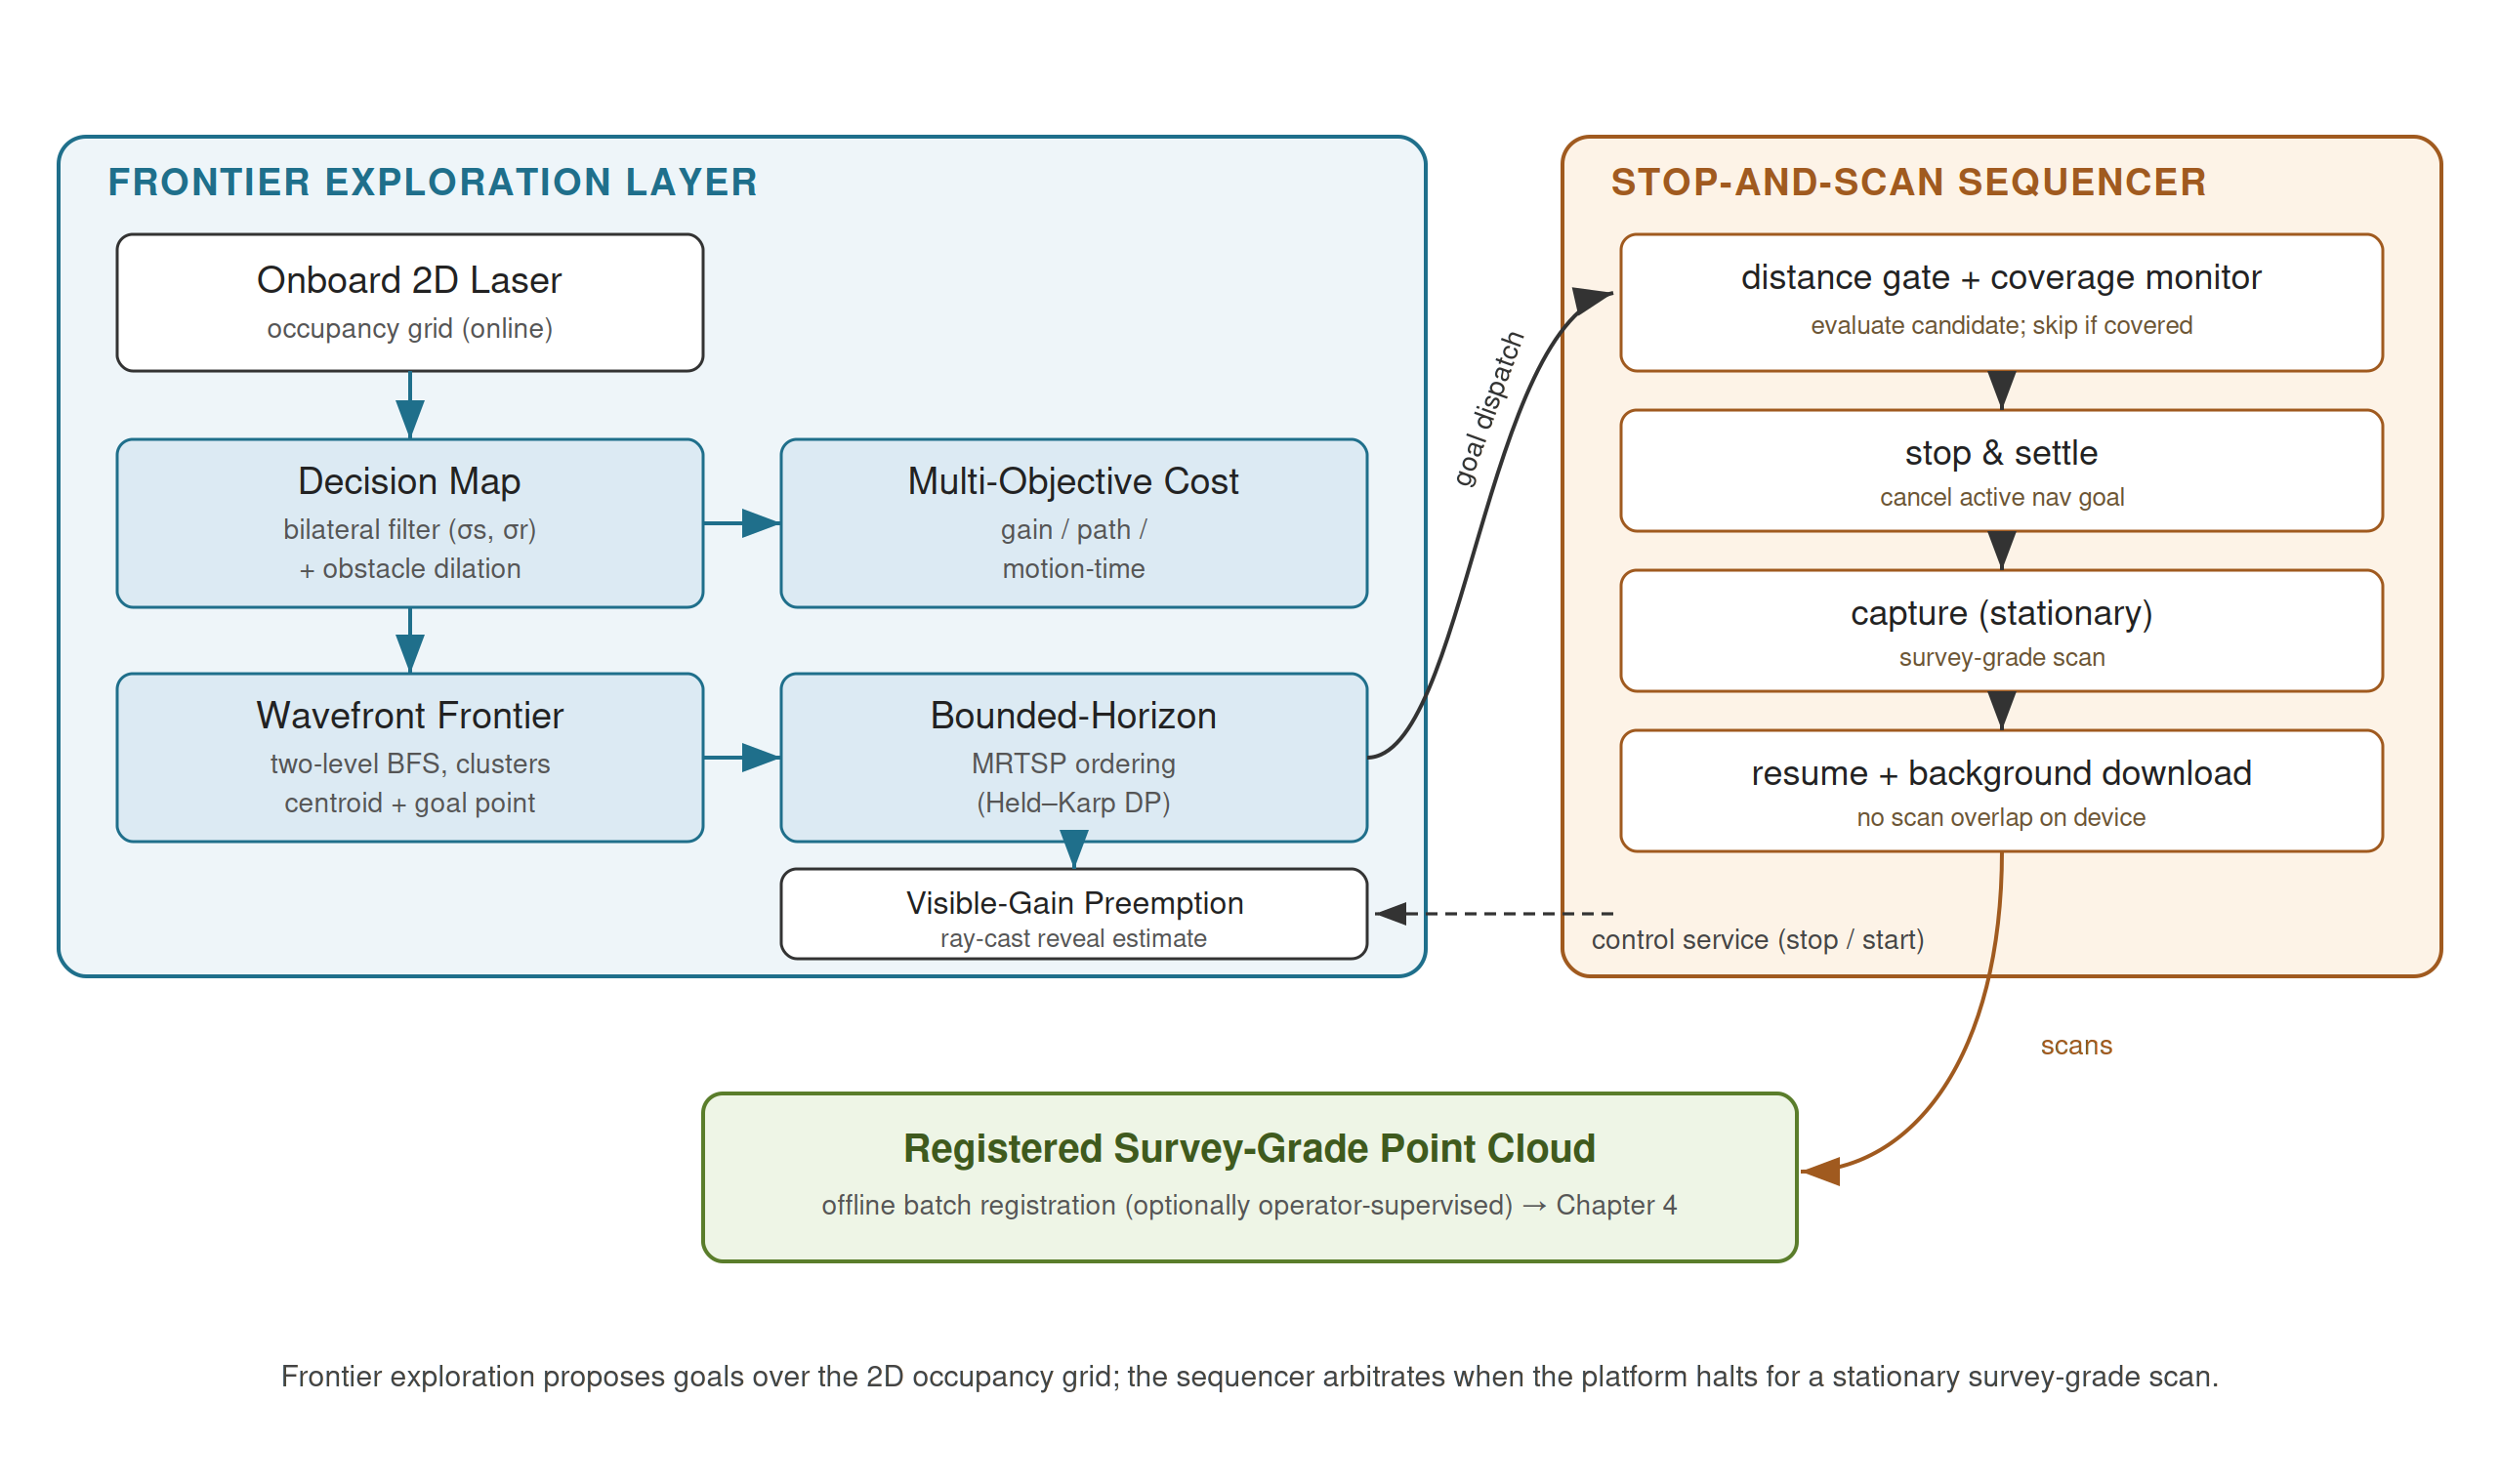
\includegraphics[width=0.95\textwidth]{figures/fig3_1.png}
  \caption{Architecture of the automated 3D mapping subsystem: the frontier
  exploration layer (decision map, wavefront detection, multi-objective cost,
  bounded-horizon ordering) and the stop-and-scan sequencer (distance gate plus
  coverage monitor), coupled through a control service.}
  \label{fig:mapping-arch}
\end{figure}

\begin{figure}[!htb]
  \centering
  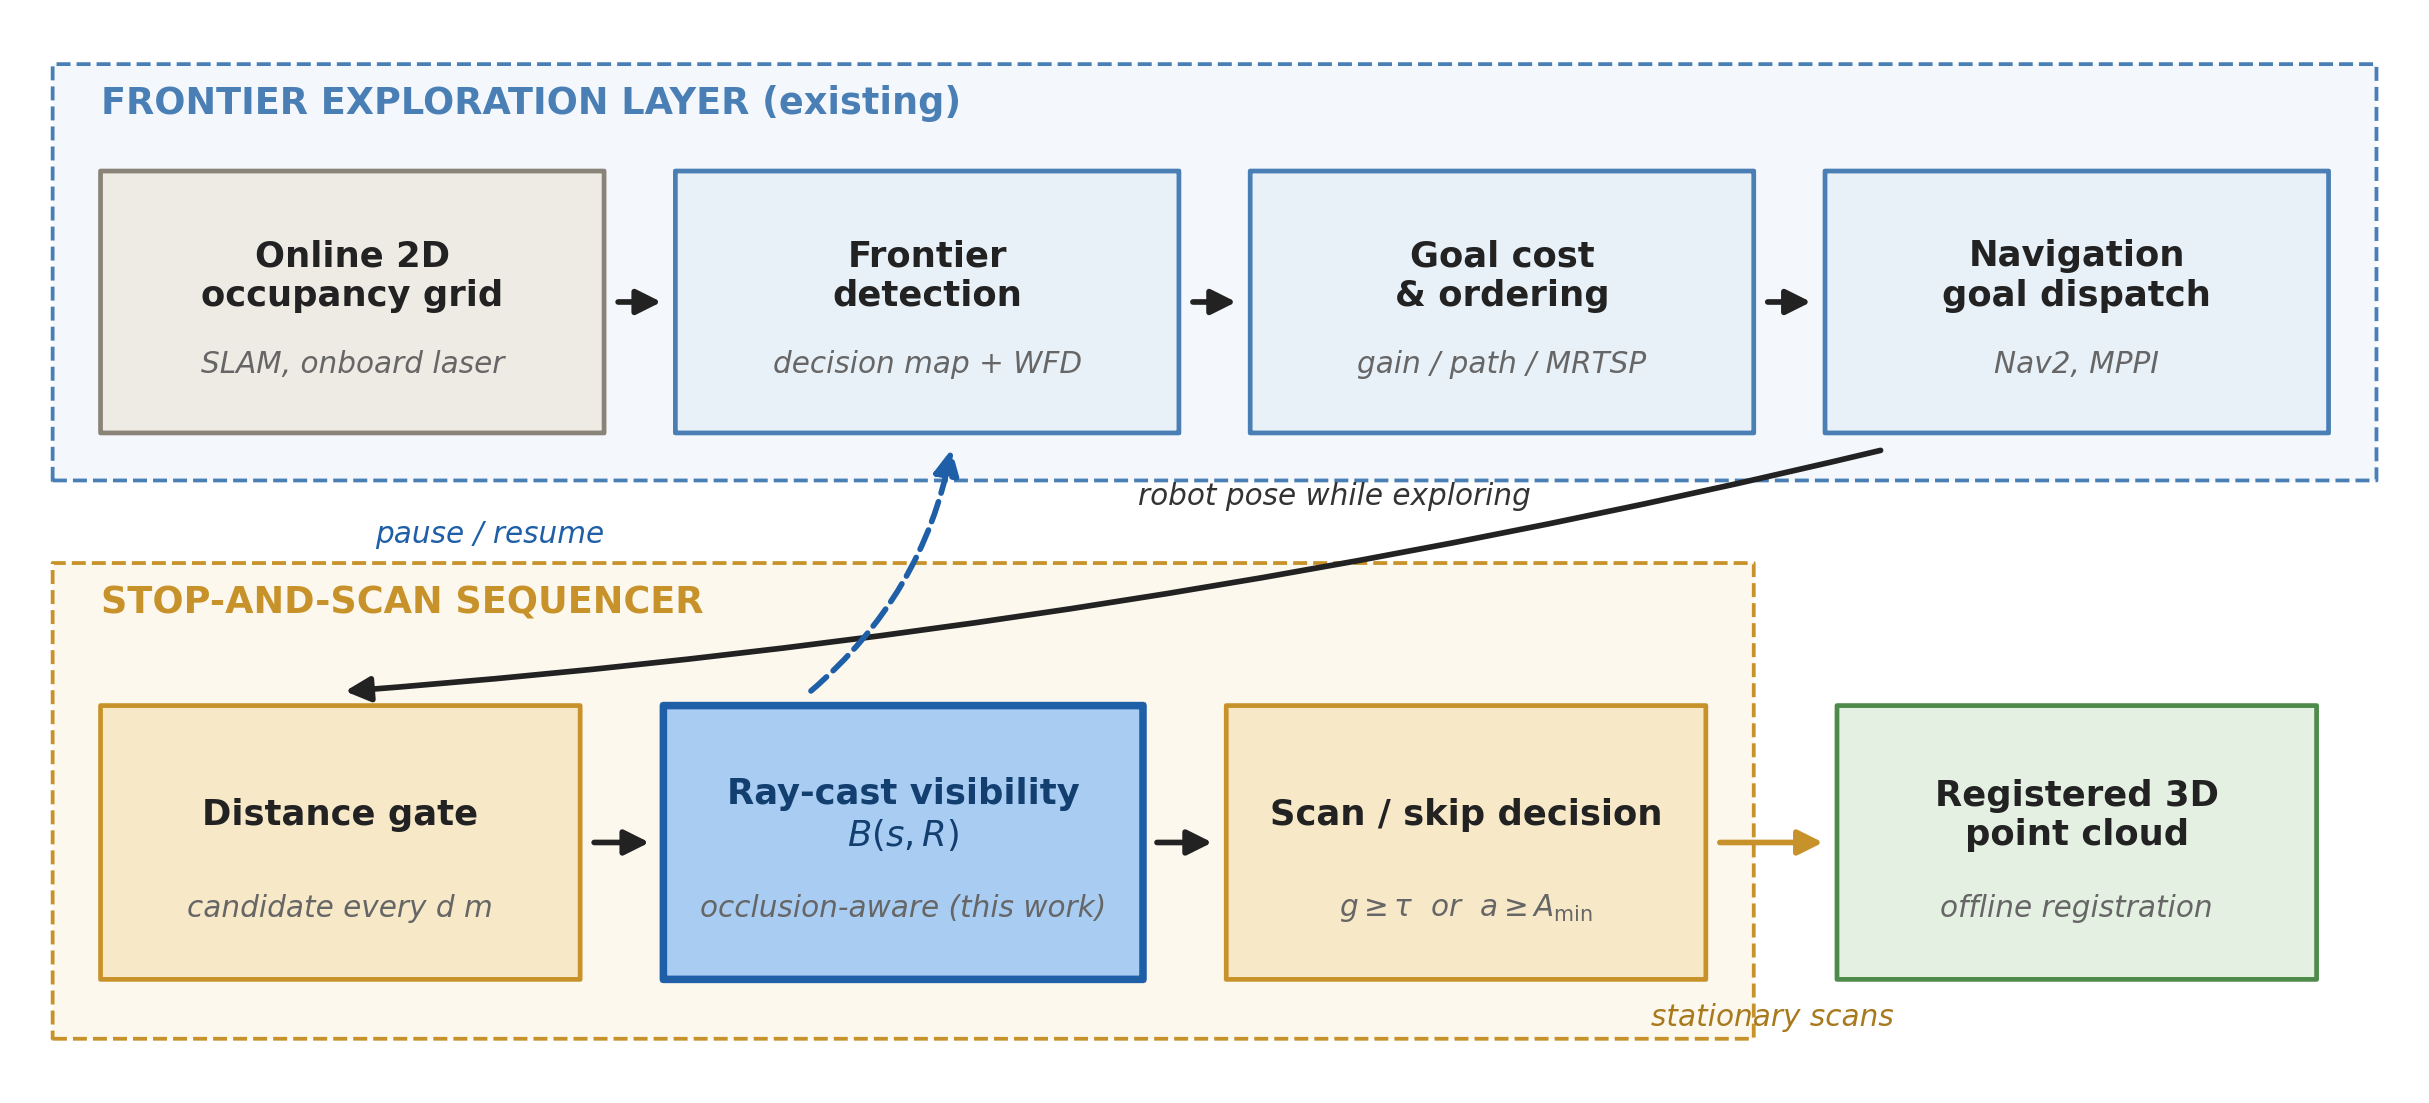
\includegraphics[width=\textwidth]{figures/sen_fig0_architecture.png}
  \caption{Data flow of the stop-and-scan-integrated frontier exploration. The
  exploration layer (top) proposes and orders navigation goals on the live
  occupancy grid; the stop-and-scan sequencer (bottom) applies the
  visibility-based scan/skip rule and triggers stationary scans that are
  registered offline.}
  \label{fig:dataflow}
\end{figure}

\section{Frontier Exploration Layer}
\label{sec:frontier-layer}

The frontier exploration layer is adopted from an open-source ROS~2 frontier
exploration package~\cite{guler2024}; its decision-map construction, wavefront
frontier detection, multi-objective cost, and bounded-horizon visit ordering
are summarized here because the stop-and-scan sequencer and the coverage model
of this dissertation are wrapped around them. The contribution of this work
lies in the stop-and-scan sequencer, the exploration monitor, the coverage
model and placement policy, the BLK360 integration, and the
offline-registration and map-conversion pipeline that orchestrate survey-grade
scans on top of this explorer.

\subsection{Decision Map Construction}
\label{subsec:decision-map}

Raw occupancy grids produced during online navigation contain speckle noise and
ragged unknown-space boundaries that destabilize frontier extraction. Before
frontiers are detected, the raw grid is transformed into a decision map through
an edge-preserving denoising stage. A joint bilateral filter~\cite{tomasi1998}
is applied over the occupancy field, combining a spatial Gaussian kernel of
standard deviation $\sigma_s$ with a range kernel of standard deviation
$\sigma_r$ that distinguishes free, occupied, and unknown cell values; this
suppresses isolated misclassifications while preserving the sharp
free--unknown boundaries on which frontier detection depends. Formally, the
filtered value at cell $p$ is the normalized weighted average over its
neighborhood $N(p)$,
\begin{equation}
  O(p) = \frac{1}{W_p}\sum_{q\in N(p)}
    \exp\!\left(-\frac{\lVert p-q\rVert^2}{2\sigma_s^2}\right)
    \exp\!\left(-\frac{\lvert I(p)-I(q)\rvert^2}{2\sigma_r^2}\right) I(q),
  \label{eq:bilateral}
\end{equation}
where $I(\cdot)$ is the raw occupancy value, $O(\cdot)$ the filtered value, and
$W_p$ the sum of the same weights, which normalizes the result so that the
filter output remains on the scale of the input. The spatial kernel radius is
set to $\lceil 2\sigma_s\rceil$ cells. A subsequent morphological dilation of
obstacles by a structuring element $B_r$ of radius $r$ enforces a conservative
clearance margin,
\begin{equation}
  O_{\mathrm{dil}}(p) = \max_{q\in B_r(p)} O(q),
  \qquad B_r(p)=\{\,q:\lVert p-q\rVert\le r\,\}.
  \label{eq:dilation}
\end{equation}
The filtered decision map is cached and regenerated only when the underlying
grid changes, so that repeated frontier queries on an unchanged map incur no
recomputation.

\subsection{Wavefront Frontier Detection}
\label{subsec:wavefront}

Frontiers---free cells adjacent to unknown space---are extracted from the
decision map using a two-level wavefront breadth-first search. An outer search
expands the navigable free region outward from the robot cell; whenever it
encounters a frontier-eligible cell, an inner search grows the complete
connected frontier cluster to which that cell belongs. Clusters smaller than a
minimum cell count are discarded as noise. For each retained cluster $F$, the
algorithm computes a centroid
\begin{equation}
  c = \frac{1}{\lvert F\rvert}\sum_{i\in F}\mathbf{x}_i,
  \qquad \mathbf{x}_i=(x_i,y_i)\in\mathbb{R}^2,
  \label{eq:centroid}
\end{equation}
used as the ranking reference point, and a representative goal point selected
as the cluster point closest to the centroid that also lies beyond a minimum
goal distance from the robot, ensuring that the dispatched goal is both
representative and reachable. If the robot projects into unknown or occupied
space, a recovery search nudges the seed to the nearest reachable free cell.

\subsection{Multi-Objective Frontier Cost}
\label{subsec:cost}

Each candidate frontier is scored through a multi-objective cost that balances
the information expected from visiting it against the effort required to reach
it. Let the information gain of a candidate be $g=\lvert F\rvert$, its cluster
size. The cost charged to the first dispatched step from the robot pose is
\begin{equation}
  c_{\mathrm{start}} = \frac{w_d\,L_{\mathrm{path}}}{g^{\,w_s}}
    + \frac{t_{\mathrm{motion}}}{\sqrt{g}},
  \label{eq:cstart}
\end{equation}
whereas a frontier-to-frontier transition in the visit sequence is charged the
distance-over-gain term only,
\begin{equation}
  c_{\mathrm{edge}}(i\!\to\! j) =
    \frac{w_d\,L_{\mathrm{path}}(i\!\to\! j)}{g_j^{\,w_s}}.
  \label{eq:cedge}
\end{equation}
Here $w_d$ is the distance weight and $w_s$ the gain exponent. The path length
$L_{\mathrm{path}}$ uses a two-point frontier approximation that discounts the
effective sensor range $r_s$,
\begin{equation}
  L_{\mathrm{path}} = \max(d_m+d_u,\; d_n+d_v) - r_s,
  \label{eq:lpath}
\end{equation}
where $d_m$ and $d_n$ are the distances from the source to the target goal
point and centroid, and $d_u$ and $d_v$ the distances from those two target
points to a start-world reference (Figure~\ref{fig:twopoint}a). The motion-time
lower bound separates translation at maximum linear speed $v_{\max}$ from
in-place rotation toward the target at maximum angular speed $w_{\max}$,
\begin{equation}
  t_{\mathrm{motion}} = \frac{D}{v_{\max}}
    + \frac{\min(\lvert\Delta\psi\rvert,\;2\pi-\lvert\Delta\psi\rvert)}{w_{\max}},
  \label{eq:tmotion}
\end{equation}
where $D$ is the translation distance and $\Delta\psi$ the heading change
required to face the target. Dividing the path term by $g^{w_s}$ and the
motion-time term by $\sqrt{g}$ makes larger, more informative clusters
cheaper, and hence preferred, while nearer candidates of comparable size
remain favored; the
sensor-range discount rewards candidates that extend coverage without redundant
overlap. The relative dominance of the two terms reverses with cluster size at
the crossover $g^*$ defined by
\begin{equation}
  g^{*\,(w_s-1/2)} = \frac{w_d\,L_{\mathrm{path}}}{t_{\mathrm{motion}}},
  \label{eq:crossover}
\end{equation}
so that for small clusters the motion-time term dominates and nearby candidates
are strongly preferred, whereas for large clusters the path term dominates and
coverage extension is rewarded. The gain exponent $w_s$ thus tunes this
crossover size to the high fixed cost of each stationary scan.
Table~\ref{tab:cost-terms} summarizes the terms.

\begin{table}[htbp]
  \centering
  \caption{Terms of the multi-objective frontier cost and their governing
  parameters.}
  \label{tab:cost-terms}
  \begin{tabularx}{\textwidth}{l X l}
    \toprule
    \textbf{Term} & \textbf{Meaning} & \textbf{Governing parameter} \\
    \midrule
    $g=\lvert F\rvert$ & Information gain proxy (frontier cluster size) & minimum frontier size \\
    $L_{\mathrm{path}}$ & Two-point frontier path approximation minus sensor reach & sensor effective range $r_s$ \\
    $t_{\mathrm{motion}}$ & Translation $+$ heading-change lower-bound time & $v_{\max}$, $w_{\max}$ \\
    $w_d$ & Distance weight on the path term & distance weight \\
    $w_s$ & Gain exponent shaping breadth vs.\ economy & gain exponent \\
    \bottomrule
  \end{tabularx}
\end{table}

\subsection{Bounded-Horizon Visit-Order Optimization}
\label{subsec:visit-order}

Selecting only the single cheapest frontier at each step is myopic and can
induce inefficient back-and-forth motion that is especially costly when every
stop incurs a multi-minute scan. The visit order is therefore optimized over a
bounded planning horizon, formulated as a single-platform bounded-horizon
traveling-salesman problem over a cost matrix whose zeroth row and column
represent a synthetic robot start node. Let $dp[S][j]$ denote the minimum cost
of a route that starts at the robot node, visits exactly the set $S$ of
frontiers, and ends at frontier $j\in S$. The Held--Karp~\cite{heldkarp1962}
recurrence is
\begin{equation}
  dp[S\cup\{j\}][j] = \min_{i\in S}\bigl(dp[S][i] + c_{\mathrm{edge}}(i\!\to\! j)\bigr),
  \qquad dp[\{j\}][j] = c_{\mathrm{start}}(j).
  \label{eq:heldkarp}
\end{equation}
The dynamic program expands one path-length layer at a time, so states whose
cardinality exceeds the planning horizon $K$ are never materialized; the
optimal $K$-step route is recovered by following parent pointers backward from
the minimum-cost terminal state. The candidate pool is pruned to a configurable
limit $N$ by $c_{\mathrm{start}}$ before the dynamic program runs, keeping the
bitmask state within a 64-frontier capacity, and a greedy nearest-by-cost
traversal is used as a fallback when the pool exceeds capacity. The number of
materialized states and the time complexity are bounded as
\begin{equation}
  \lvert\text{states}\rvert = \sum_{k=1}^{K}\binom{N}{k}\,k = O(2^K K),
  \qquad \text{time} = O(2^K K^2),
  \label{eq:complexity}
\end{equation}
so keeping $K$ small makes real-time replanning feasible even when each stop
takes several minutes (Figure~\ref{fig:twopoint}b).

\begin{figure}[!htb]
  \centering
  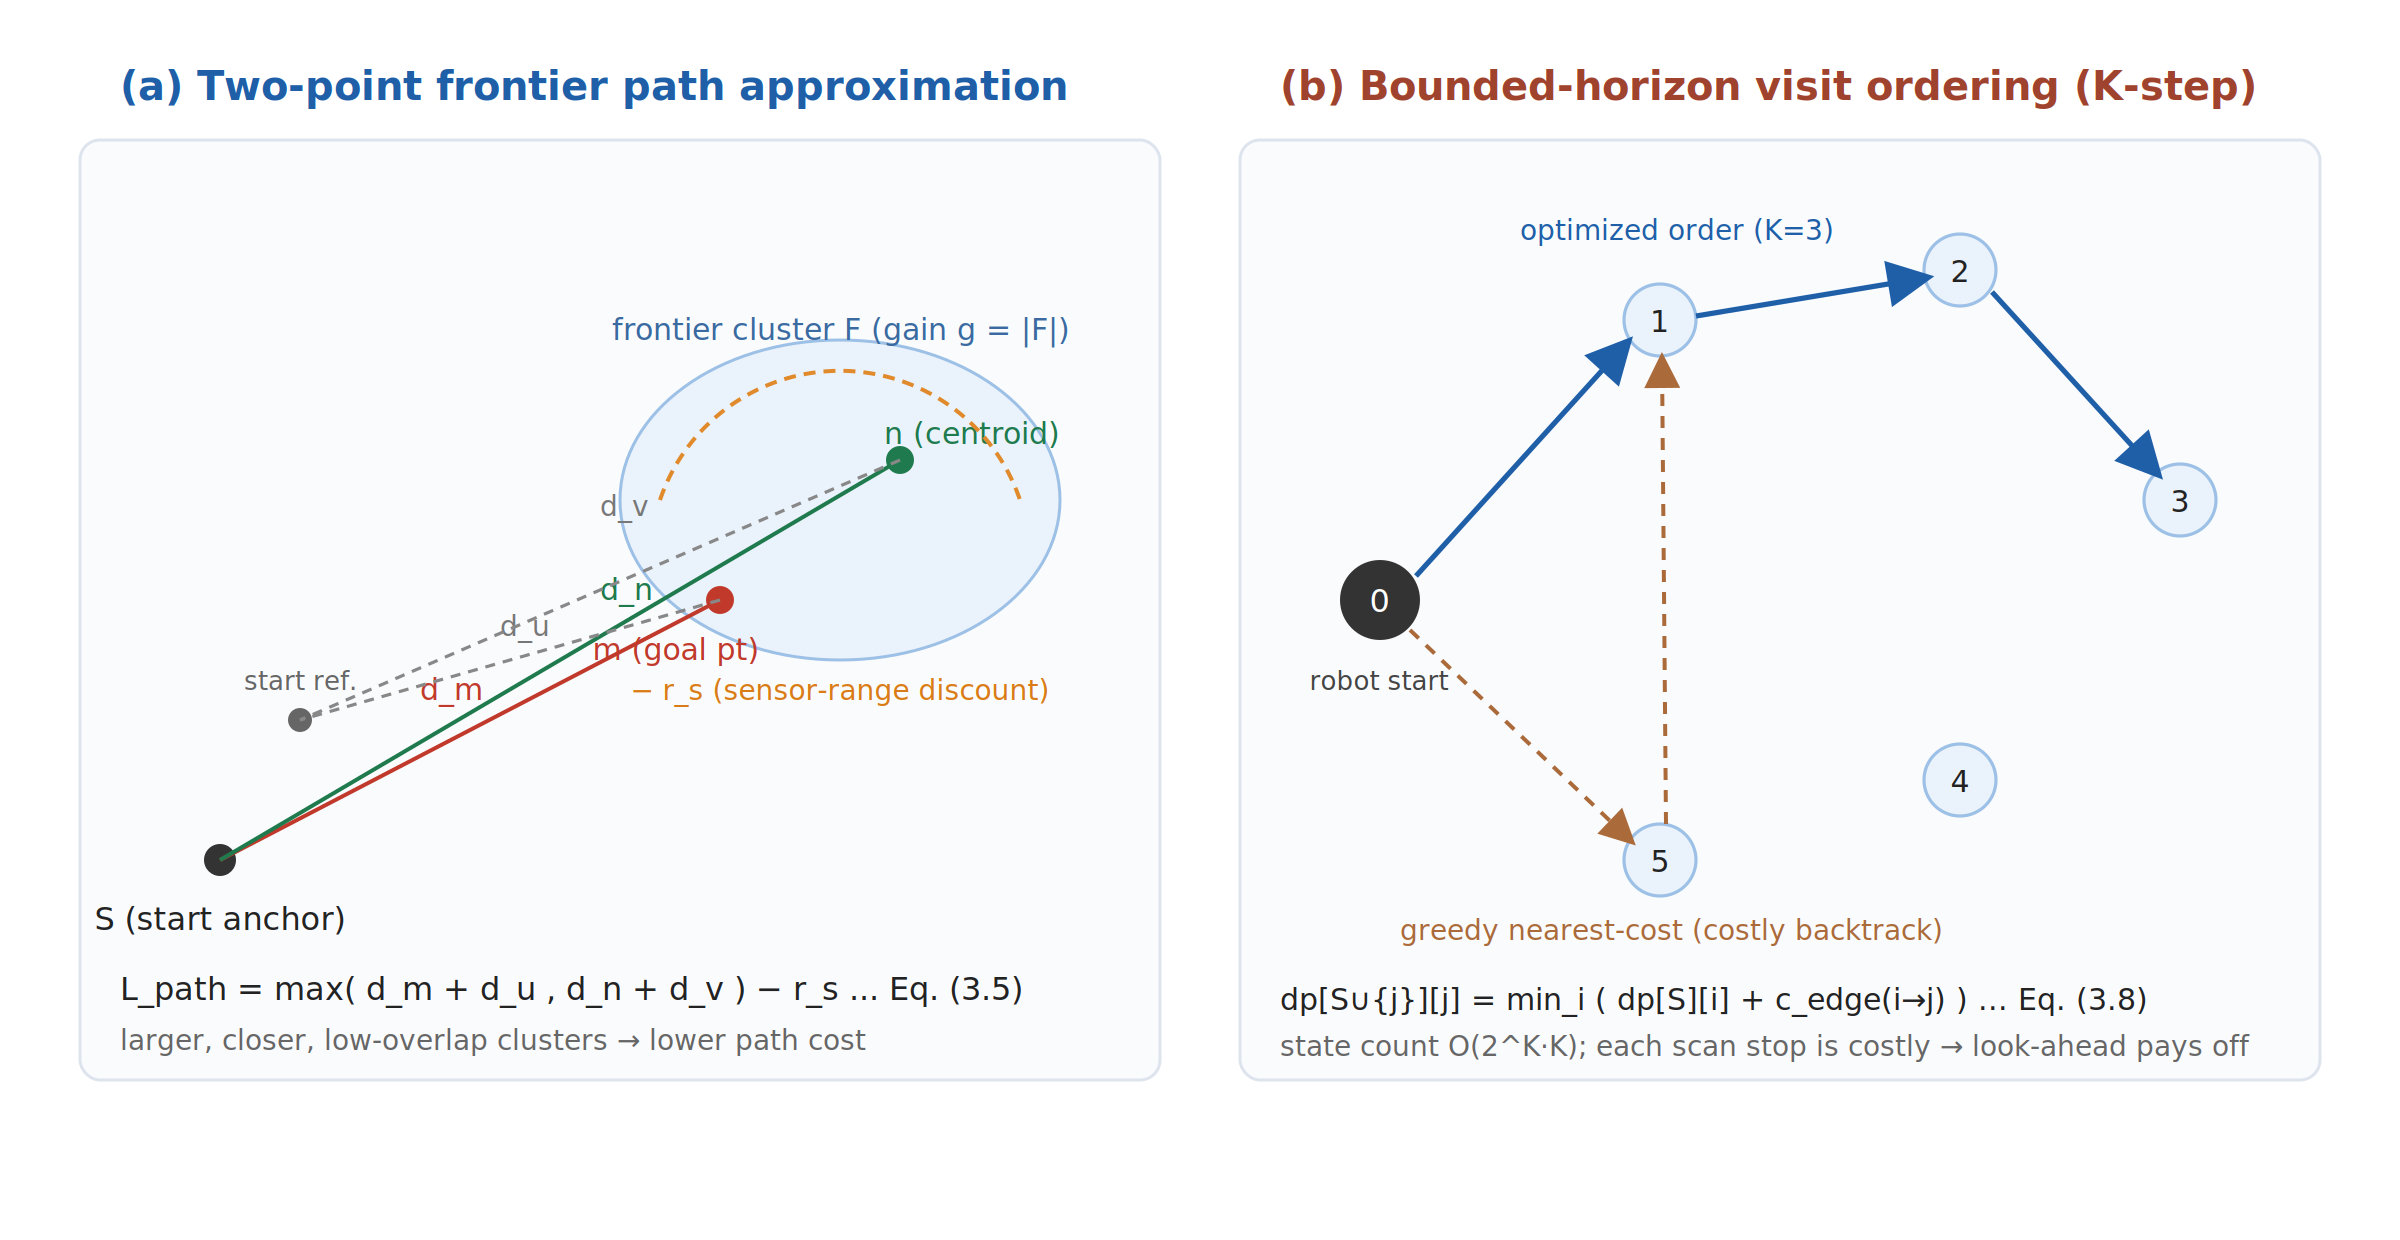
\includegraphics[width=0.92\textwidth]{figures/fig3_4.png}
  \caption{(a) Two-point frontier path approximation
  (Equation~\ref{eq:lpath}): the effective sensor range $r_s$ is discounted
  from the distances to the goal point $m$ and centroid $n$ from the start
  anchor. (b) Bounded-horizon visit ordering (Equation~\ref{eq:heldkarp}):
  because each stationary scan is costly, $K$-step look-ahead reduces the
  backtracking of greedy selection.}
  \label{fig:twopoint}
\end{figure}

\section{Stop-and-Scan Sequencing}
\label{sec:sequencing}

\subsection{Sequencer State Machine}
\label{subsec:fsm}

The stop-and-scan sequencer governs when survey-grade acquisitions occur. It is
structured as a finite-state machine with the states EXPLORING, STOPPING,
SCANNING, RECONNECT, and RESUMING (Figure~\ref{fig:fsm}). During EXPLORING, the
frontier layer drives the platform while the sequencer monitors the net
straight-line displacement of the robot in the map frame from the last
evaluation reference position $q$. A scan \emph{candidate} is raised when
\begin{equation}
  \lVert p_t - q\rVert_2 \ge d,
  \label{eq:distance-gate}
\end{equation}
where $p_t$ is the current platform position and $d$ is the candidate
interval; the reference $q$ is initialized to the start pose and advanced at
every raised candidate whether or not it is accepted. Because this is net displacement rather than path length, dwelling or
circling in place raises no candidate. When a candidate is accepted by the
placement rule of Section~\ref{sec:placement}, the sequencer transitions to
STOPPING, halts the active navigation goal through the control service, and
waits until the platform comes to rest. It then enters SCANNING, triggers a
survey-grade acquisition, and waits for a capture confirmation. Because the
scanner separates a stationary capture phase from a subsequent background
download phase, the sequencer resumes exploration once the capture is
confirmed, allowing the platform to drive toward the next scan point while the
previous scan downloads; two scans are never allowed to overlap on the device,
\begin{equation}
  [\,t_c,\,t_c+\tau_c\,] \,\cap\, [\,t_d,\,t_d+\tau_d\,] = \varnothing,
  \label{eq:no-overlap}
\end{equation}
where $t_c$ and $t_d$ are the capture and download start times and $\tau_c$
and $\tau_d$ the corresponding durations.
Acquisition failures or link drops transition the machine to RECONNECT, which
retries the acquisition up to a bounded number of attempts before either
resuming or aborting.

\begin{figure}[!htb]
  \centering
  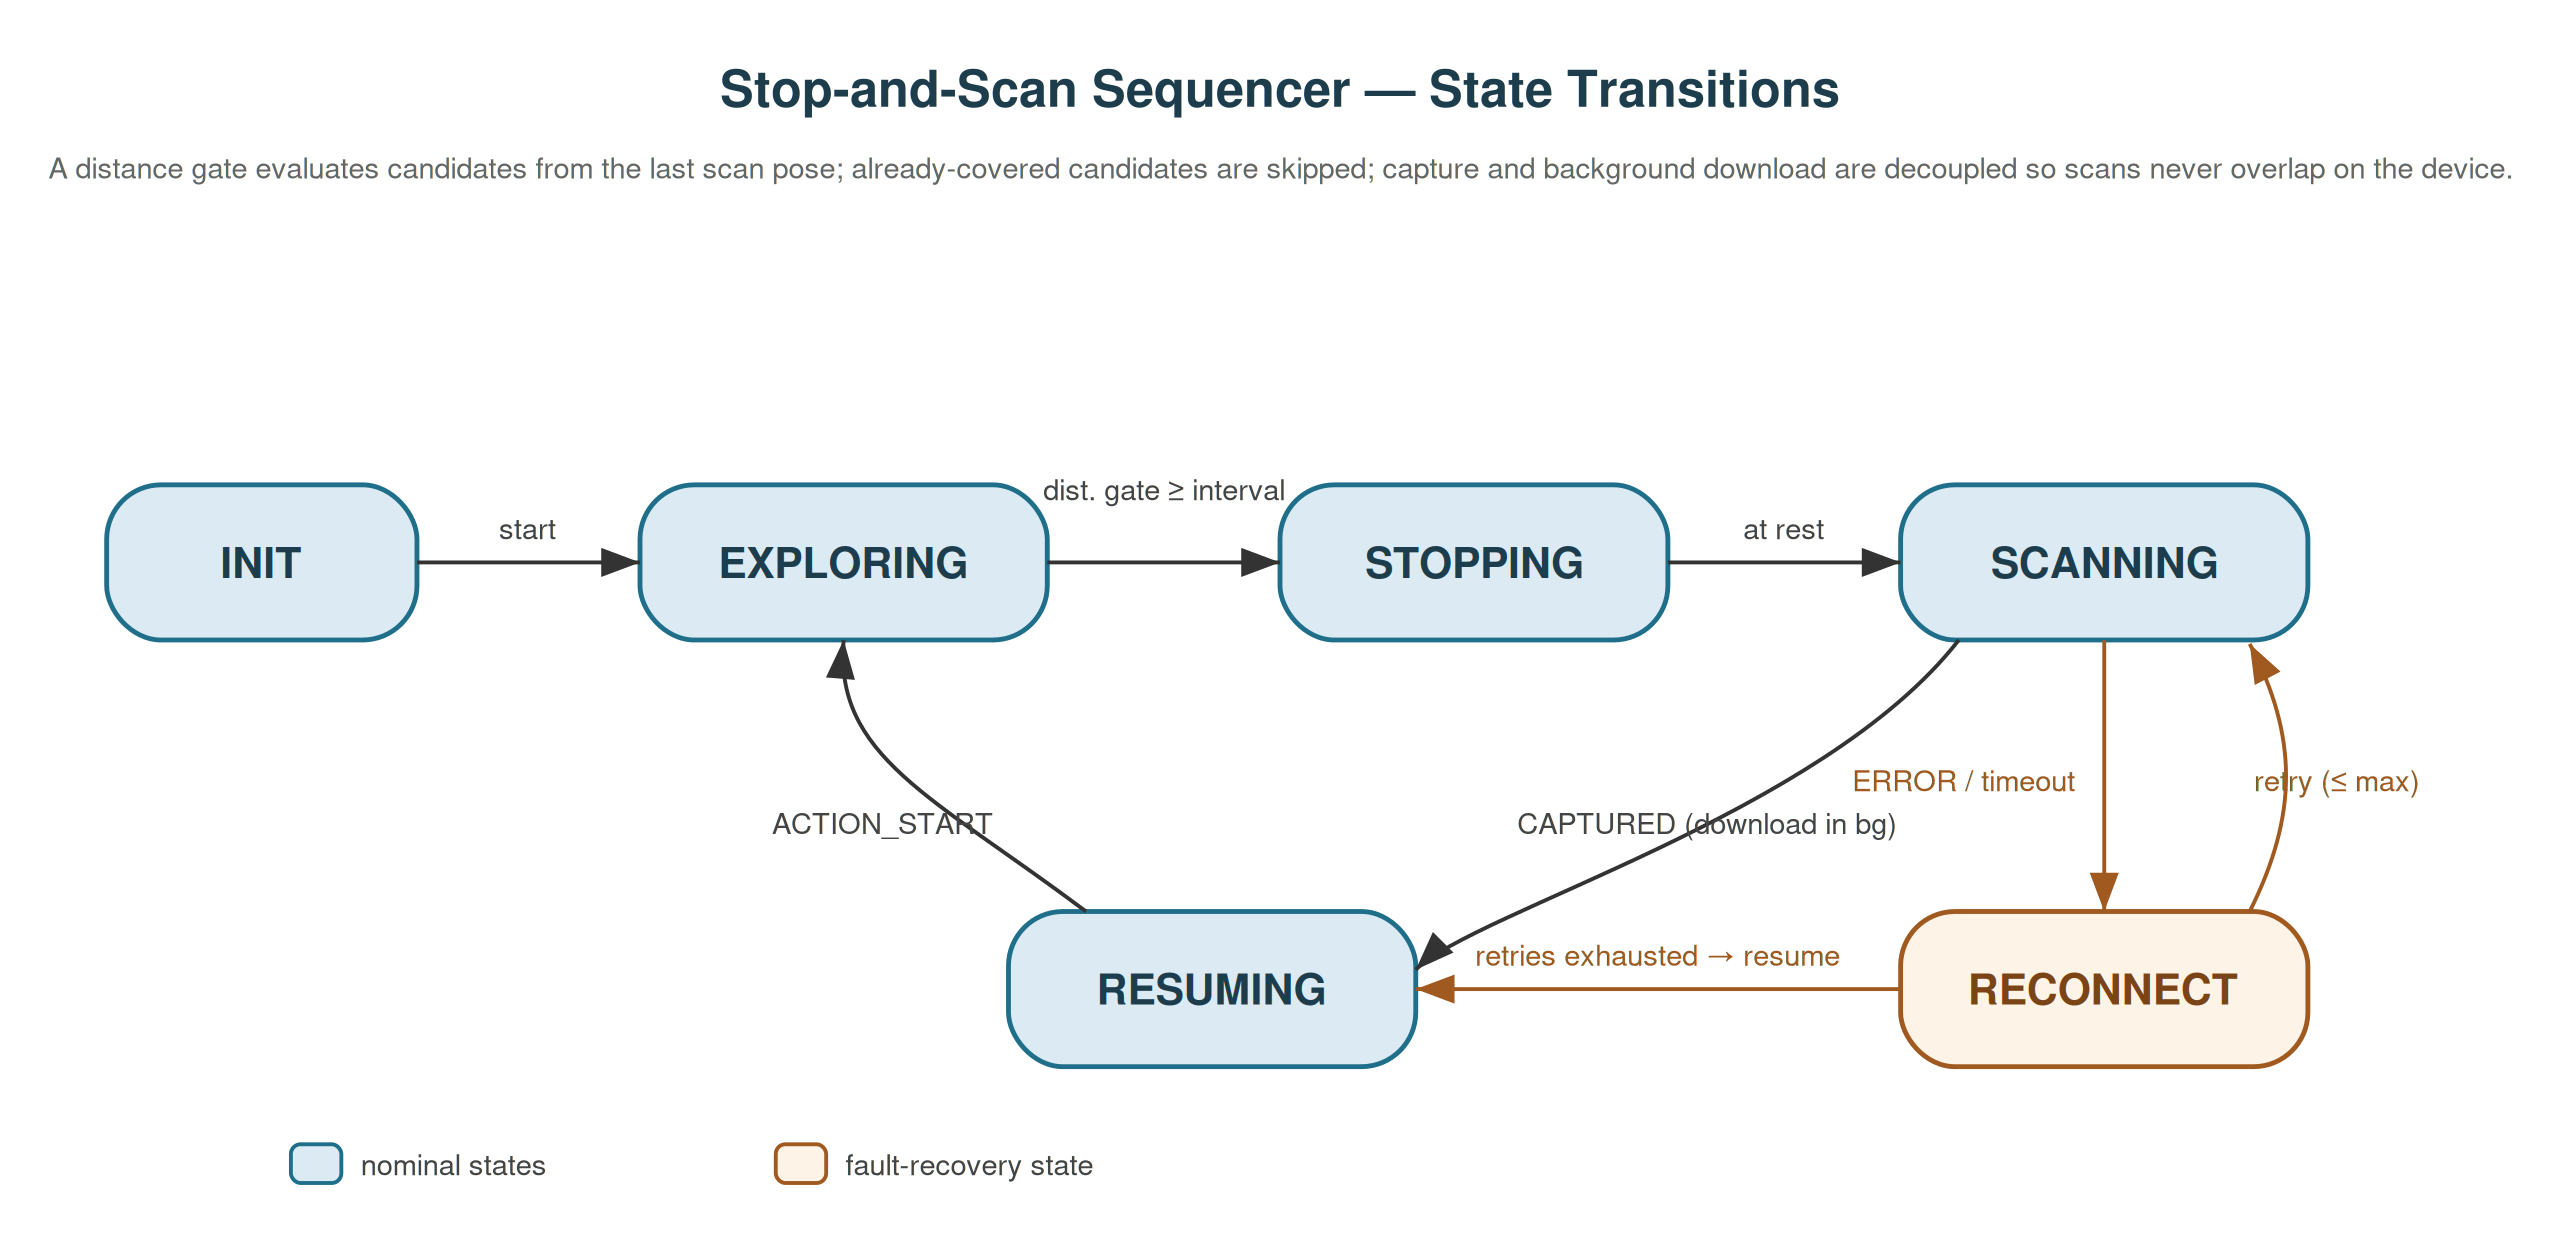
\includegraphics[width=0.95\textwidth]{figures/fig3_2.png}
  \caption{State-transition diagram of the stop-and-scan sequencer: INIT $\to$
  EXPLORING $\to$ STOPPING $\to$ SCANNING $\to$ (RECONNECT) $\to$ RESUMING
  $\to$ EXPLORING, with a distance gate, a coverage-based scan/skip decision,
  and capture--download decoupling.}
  \label{fig:fsm}
\end{figure}

\subsection{Goal Preemption and Frontier Suppression}
\label{subsec:preemption}

During navigation toward a frontier goal, newly revealed map information may
render the active goal redundant before the platform arrives. The subsystem
therefore applies a visible-gain goal-preemption test. Using a ray-casting
sensor model from the prospective goal pose, parameterized by an effective
range, a field of view, and an angular ray step, the subsystem counts how many
genuinely unknown frontier cells would still be revealed from that pose; rays
terminate at occupied cells or at the local cluster bounds, and each revealed
cell is counted at most once,
\begin{equation}
  G_{\mathrm{vis}}(p) = \bigl\lvert\{\,\text{first unknown frontier cell hit by ray }k\,\}\bigr\rvert,
  \qquad L_{\mathrm{reveal}} = G_{\mathrm{vis}}\cdot\Delta r,
  \label{eq:preempt}
\end{equation}
where $\Delta r$ is the map resolution that converts the cell count into a
reveal-length estimate. If $L_{\mathrm{reveal}}$ falls below a threshold, or
the platform is already within a completion radius of the goal, the active
goal is preempted and the next goal in the optimized sequence is dispatched. A
minimum time interval between preemptions prevents goal churn. A complementary
frontier-suppression mechanism temporarily blacklists clusters that repeatedly
fail to make progress, expanding a suppression region around them and pruning
expired suppressions over time, so that the explorer does not fixate on
unreachable frontiers.

\subsection{Exploration Termination}
\label{subsec:termination}

Exploration termination is decided by two independent criteria. The first is
the explorer's native frontier exhaustion: when no reachable, qualifying
frontier remains after suppression and an escape-mode retry, a completion event
is fired. The second is the stall detection of the exploration monitor
implemented in this work: while actively exploring, if the count of known cells
in the occupancy grid grows by less than a minimum progress margin over a fixed
window, the map is treated as converged and termination is declared. The stall
clock is frozen during scan and download pauses so that a long scan is never
mistaken for convergence. This criterion requires no ground truth. The monitor
publishes the remaining frontier count and a latched completion flag, and logs
an end-of-run summary of elapsed time, number of scans, skipped candidates, and
completed downloads; these are the quantities reported in
Section~\ref{sec:exp-mapping}.

\subsection{Proximity-Based Scan/Skip Rule (Baseline)}
\label{subsec:proximity-rule}

The preliminary version of the sequencer~\cite{iccas2026} decided whether to
scan or skip a candidate by a proximity test. Let $S=\{s_1,\dots,s_n\}$ be the
positions actually scanned so far and define the nearest-scan distance of a
candidate position $p$ as $D(p)=\min_{s_i\in S}\lVert p-s_i\rVert_2$ (with
$D(p)=+\infty$ when $S=\varnothing$). The rule scans when $D(p)\ge R$ and skips
when $D(p)<R$, where $R$ is an effective coverage radius set with reference to
the scanner's range; equivalently, it skips whenever the candidate falls inside
the union of disks of radius $R$ around previous scans. This is the
\emph{disk spacing rule} of stop-and-go practice. It is retained in this
dissertation as the baseline against which the visibility-based rule is
evaluated, and Section~\ref{subsec:prelim-mapping} reports the scan-trigger
comparison that first motivated a coverage-based skip decision at all: without
any redundancy check, a distance-traveled trigger fires a stationary scan at
every travel interval and maps the test room with seven times more scans than
necessary.

\section{Coverage Models for Stop-and-Scan Placement}
\label{sec:coverage}

This section defines the coverage model at the core of the scan/skip decision.
The workspace is formalized on an occupancy grid, the isotropic disk model is
contrasted with the proposed ray-cast visibility region, and the line-of-sight
coverage metric is defined.

\subsection{Workspace and Notation}
\label{subsec:notation}

Let the environment be represented by a 2D occupancy grid~\cite{elfes1989,thrun2005}
$\mathcal{M}$ produced online by SLAM. The grid is an $H\times W$ array of
square cells of side $\rho$ (the grid resolution, $\rho=0.05$~m in all
experiments); each cell $c$ is identified with its center point in the map
frame. Each cell carries an integer value $o(c)$, where $o(c)=-1$ denotes
unmapped space and $o(c)\in[0,100]$ is a scaled occupancy probability. Cells
are classified as
\begin{equation}
\mathrm{state}(c)=
\begin{cases}
\textit{free}, & 0 \le o(c) \le \theta_{\mathrm{free}}, \\
\textit{occupied}, & o(c) \ge \theta_{\mathrm{occ}}, \\
\textit{unknown}, & o(c)=-1 \ \text{or}\ \theta_{\mathrm{free}}<o(c)<\theta_{\mathrm{occ}},
\end{cases}
\label{eq:state}
\end{equation}
with $\theta_{\mathrm{free}}=25$ and $\theta_{\mathrm{occ}}=65$, the
long-standing free/occupied convention of the ROS occupancy-map
pipeline~\cite{macenski2020marathon}. The classification is insensitive to the
exact placement of these values because SLAM-estimated occupancies are strongly
bimodal. The two thresholds are deliberately separated: a cell is treated as
free only when its occupancy is confidently low and as an obstacle only when
confidently high; the intermediate band is treated as unknown so that ambiguous
cells are neither counted as covered nor allowed to pass a sight line. The
set of mapped free cells, the region over which coverage is evaluated, is
written $\mathcal{F}=\{c\in\mathcal{M}:\mathrm{state}(c)=\textit{free}\}$. A
\emph{scan pose} is a stationary viewpoint $s_i\in\mathcal{F}$ at which the
platform halts and the stop-and-scan sensor acquires data; each sensor is
characterized by a range bound $R$ out to which its visibility region is
evaluated. Throughout, $s_i$ denotes an accepted scan pose, $p$ a candidate
pose under evaluation, and $c$ a grid cell.

\subsection{Isotropic Disk Coverage (Baseline)}
\label{subsec:disk}

A widely adopted and computationally convenient assumption is that a scan pose
covers every free cell within its range, giving the \emph{isotropic disk}
model
\begin{equation}
B_{\mathrm{disk}}(s_i,R)=\{c\in\mathcal{F}:\lVert c-s_i\rVert \le R\}.
\label{eq:disk}
\end{equation}
The disk model depends only on the range bound, is trivial to evaluate, and
is adequate in open, obstacle-free space. Its defining limitation is that it
ignores occlusion: because membership depends solely on proximity,
$B_{\mathrm{disk}}$ claims cells within range $R$ that are separated from $s_i$
by a wall or partition, i.e., cells to which the sensor has no line of sight
(Figure~\ref{fig:concept}a). At the placement stage, a rule that trusts
$B_{\mathrm{disk}}$ treats such a region as satisfied and skips the scan that
genuine observation would require.

\begin{figure}[!htb]
\centering
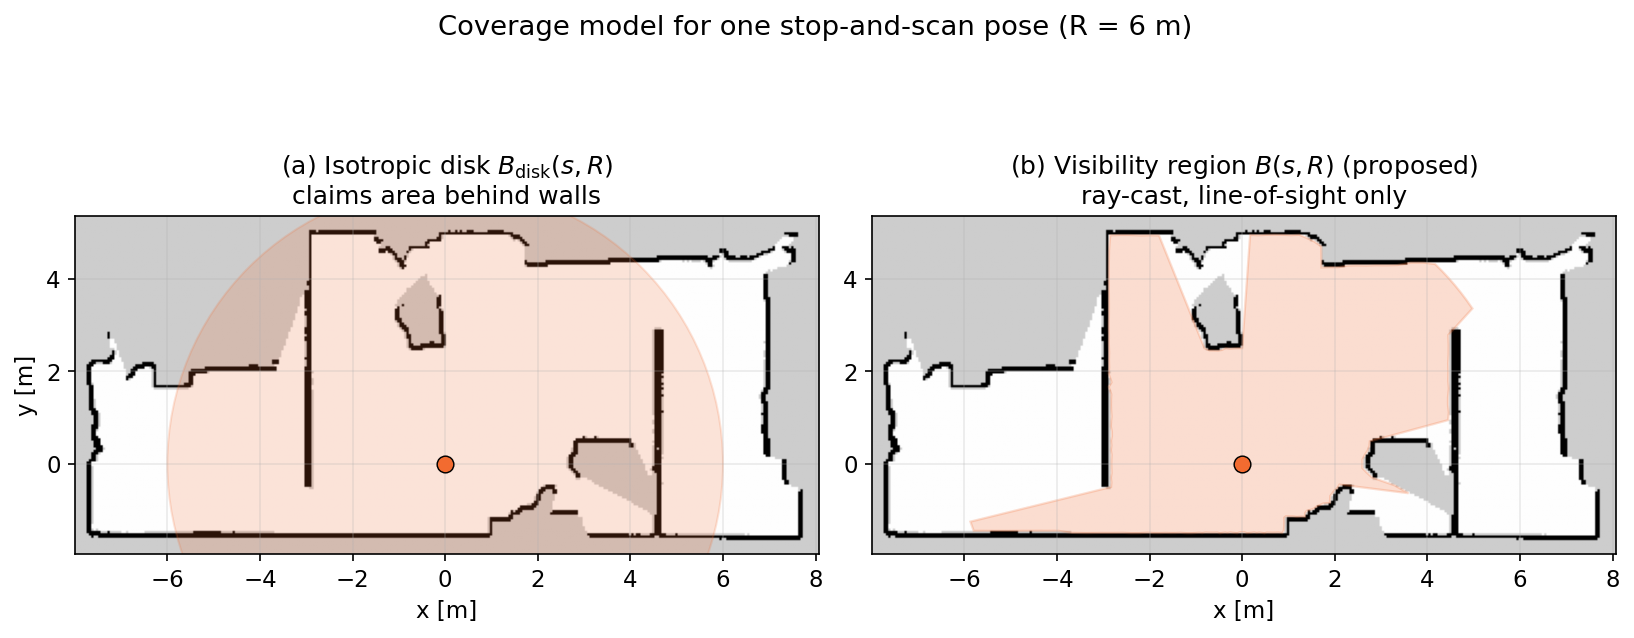
\includegraphics[width=0.85\linewidth]{figures/sen_fig1_concept.png}
\caption{Coverage models for a single scan pose ($R=6$~m). (a)~The isotropic
disk $B_{\mathrm{disk}}(s,R)$ counts every free cell within range as covered,
bleeding through walls. (b)~The proposed ray-cast visibility region $B(s,R)$
claims only genuine line-of-sight area.}
\label{fig:concept}
\end{figure}

\subsection{Ray-Cast Visibility Region (Proposed)}
\label{subsec:visibility}

To account for occlusion, the disk is replaced with a \emph{ray-cast
visibility region}, a discrete visibility polygon that admits only cells in
direct line of sight of the scan pose. From $s_i$, $N_r=720$ rays are cast over a
full $360^\circ$ field at uniform angular resolution
$\Delta\theta=0.5^\circ$. Each ray is marched outward in steps of half a cell
and is truncated at the first sample that is either occupied or unknown; that
terminating cell and everything beyond it on the ray are excluded. Formally,
for a free cell $c$ on the ray at azimuth $\theta_k$, let $\overline{s_i c}$
denote the cells strictly between $s_i$ and $c$ along the ray. Then
\begin{equation}
B(s_i,R)=\left\{c\in\mathcal{F}:
\lVert c-s_i\rVert \le R \ \wedge\
\mathrm{state}(c')=\textit{free}\ \ \forall\, c'\in\overline{s_i c}\right\}.
\label{eq:visibility}
\end{equation}
A free cell is claimed as covered only if every intervening cell along the
sight line to it is also mapped free space. Occupied cells terminate the ray
because the obstacle blocks the beam, and unknown cells terminate it because
the model refuses to assert visibility through unmapped space. This second
condition is deliberately conservative: the model never ``sees through''
regions the map cannot vouch for. The set definition characterizes the ideal
geometric visibility region and does not depend on the ray discretization; the
$K$ rays and half-cell marching are the implementation that approximates it. At
the range bound the inter-ray arc spacing is $R\,\Delta\theta\approx5.2$~cm for
$R=6$~m, on the order of a single grid cell, so the discrete approximation
recovers the ideal region up to single-cell effects at region boundaries. By
construction $B(s_i,R)\subseteq B_{\mathrm{disk}}(s_i,R)$ for any pose and
range: ray-casting can only remove cells the disk would have claimed, and the
two coincide only for an obstacle-free disk around $s_i$
(Figure~\ref{fig:concept}b). Each visibility polygon is computed in pure array
operations in roughly 2~ms, inexpensive enough to evaluate at every scan
candidate online.

\subsection{Line-of-Sight Coverage Metric}
\label{subsec:los}

Coverage by a set of scan poses is the union of their visibility regions. For
$S=\{s_1,\dots,s_n\}$ the covered area is $C(S)=\bigcup_{i=1}^{n} B(s_i,R)$,
and the \emph{line-of-sight (LOS) coverage} is the fraction of mapped free
space observed from at least one scan pose,
\begin{equation}
\mathrm{LOS}(S)=\frac{\lvert C(S)\cap\mathcal{F}\rvert}{\lvert\mathcal{F}\rvert}\in[0,1],
\label{eq:los}
\end{equation}
where $\lvert\cdot\rvert$ counts cells. The complement $1-\mathrm{LOS}(S)$
corresponds to mapped free cells that remain occluded from every scan pose.
Because the metric is defined over $\mathcal{F}$ and visibility never
propagates through occupied or unknown cells, LOS coverage is a conservative
measure of genuine observation rather than the optimistic proximity count
produced by the disk model. It is the single figure of merit reported for
scan placement in Section~\ref{sec:exp-mapping}.

\subsection{Scope: 2D Station Planning for 3D Mapping}
\label{subsec:scope2d}

The visibility model and the LOS metric are deliberately 2D: they
reason on the live occupancy grid, a horizontal slice of the environment at the
mapping sensor's height. LOS coverage therefore certifies sight lines to
floor-space cells, not to the full 3D surface set the scanner observes.
Vertical occlusions---shelves, overhanging structures, elevated machinery, or
surfaces stacked at different heights above the same floor cell---are not
represented, and high 2D LOS coverage does not by itself guarantee complete 3D
surface coverage. This scope is a design choice matched to the online setting:
the occupancy grid is what SLAM makes available in real time on the platform;
the 2D visibility polygon is cheap enough to evaluate at every candidate; and
in the room-scale indoor environments targeted here, a pose with unobstructed
2D line of sight to a floor region generally also observes much of the
structure above it, because the scanner acquires a full dome. The contribution
should accordingly be read as occlusion-aware 2D scan-station planning for
subsequent 3D mapping; a genuinely 3D visibility representation is future work
(Chapter~\ref{ch:conclusion}).

\section{Visibility-Based Placement Policy}
\label{sec:placement}

Section~\ref{sec:coverage} defined what a scan pose observes; this section
defines where the robot decides to stop and scan. Because each stationary scan
carries a large fixed cost, the placement policy must take as few scans as
possible while maintaining high LOS coverage (Equation~\ref{eq:los}) of the
mapped free space.

\subsection{Marginal Visibility Gain}
\label{subsec:gain}

Let $S=\{s_1,\dots,s_n\}$ be the scans accepted so far and
$C(S)=\bigcup_i B(s_i,R)$ their union coverage. The visibility regions of
previously accepted scans are not frozen: at every decision, $C(S)$ is
recomputed on the current occupancy map, so earlier regions expand or contract
as SLAM refines the map. For a candidate pose $p$ raised by the distance gate
(Equation~\ref{eq:distance-gate}), the decision is based on how much \emph{new}
line-of-sight area its visibility region contributes relative to what it sees
in total. The \emph{normalized marginal gain} and the \emph{absolute new
area} are
\begin{equation}
g(p\mid S)=\frac{\lvert B(p,R)\setminus C(S)\rvert}{\lvert B(p,R)\rvert},
\qquad
a(p\mid S)=\lvert B(p,R)\setminus C(S)\rvert\cdot\rho^2,
\label{eq:gain}
\end{equation}
with $g\in[0,1]$ and $a$ in m$^2$. Both quantities are evaluated directly on
the visibility regions, so occlusion is respected: area behind a wall is never
part of $B(p,R)$ and never inflates either the coverage or the gain. A
candidate whose visibility region is degenerate (smaller than 0.5~m$^2$, which
occurs when the pose projects into an obstacle or an unmapped pocket) is
rejected outright before the gain is evaluated, so the denominator never
vanishes.

\subsection{Dual-Criterion Accept/Skip Rule}
\label{subsec:dual}

A naive policy would accept a candidate whenever its relative gain exceeds a
threshold, $g\ge\tau$. This single relative test is fragile for a
room-scale stop-and-scan sensor: because $R$ is comparable to the size of a
room, $B(p,R)$ is large, so a small but genuinely occluded pocket
contributes only a tiny fraction of that region and fails the relative test,
even though it is exactly the kind of unscanned area the method exists to
capture. A candidate is therefore accepted when \emph{either} a relative
\emph{or} an absolute criterion is met,
\begin{equation}
\textsf{scan}(p)\iff
\big(g(p\mid S)\ge\tau\big)\ \lor\ \big(a(p\mid S)\ge A_{\min}\big),
\label{eq:dual}
\end{equation}
and skipped only when both fail. The relative term $\tau$ captures candidates
that open a large new area such as a previously unseen room; the absolute term
$A_{\min}$ rescues small but real occlusion pockets whose new area is a
negligible fraction of the scanner's footprint. The experiments use
$\tau=0.30$ and $A_{\min}=5$~m$^2$ with range bound $R=6$~m;
Section~\ref{subsec:exp-sensitivity} shows that coverage and scan count are
nearly flat in $\tau$ over $[0.10,0.50]$, whereas $A_{\min}$ is the operative
knob trading coverage against scan count, with its knee at 5~m$^2$.

Two disk-based baselines are evaluated against this rule. The first is the
proximity spacing rule of Section~\ref{subsec:proximity-rule}. This rule is
\emph{not} mathematically equivalent to the marginal-gain rule applied to
$B_{\mathrm{disk}}$---a candidate closer than $R$ to an existing scan can still
contribute a crescent of new disk area---so a comparison against it changes
both the coverage model and the acceptance rule. To isolate the coverage model
itself, the ablation of Section~\ref{subsec:exp-ablation} additionally
evaluates a \emph{disk marginal-gain} baseline that applies the identical dual
criterion (Equation~\ref{eq:dual}) with $B_{\mathrm{disk}}$ substituted for
$B$; within that pair, the only difference is the coverage model.

\subsection{Coverage-Completion Phase}
\label{subsec:completion}

Frontier-driven exploration terminates when the known map stops growing
(Section~\ref{subsec:termination}), but convergence of the \emph{map} does not
by itself guarantee that every mapped free cell has been brought into line of
sight: small occluded pockets can remain. The method therefore includes an
optional coverage-completion phase that runs after exploration converges. The
uncovered free cells $\mathcal{F}\setminus C(S)$ are clustered into connected
pockets; for each pocket of area at least $A_{\mathrm{pocket}}$, the robot
navigates into the pocket and takes a stationary scan, repeating until no
qualifying pocket remains. The phase is bounded by per-pocket navigation
timeouts, an overall scan budget, and a list of pockets found unreachable, so
it always terminates. The method does not claim 100\% LOS coverage:
sub-$A_{\mathrm{pocket}}$ fragments at wall and obstacle edges are reported as
residual rather than rounded up.

\subsection{Integration with Exploration}
\label{subsec:integration}

The placement policy is embedded in the autonomous exploration loop without
owning the navigation goals. The frontier explorer drives the robot toward
unmapped space on the live occupancy map; the sequencer monitors displacement,
applies the accept/skip rule at each raised candidate, and triggers a stationary
scan when a candidate is accepted, resuming exploration afterward. Completion
is declared by the exploration monitor, after which the optional
coverage-completion phase runs and the run is finalized.
Algorithm~\ref{alg:placement} summarizes the complete placement policy.

\begin{algorithm}[H]
\caption{Visibility-based stop-and-scan placement}
\label{alg:placement}
\begin{algorithmic}[1]
\Require live occupancy map $\mathcal{M}$; range bound $R$; thresholds $\tau$, $A_{\min}$, $A_{\mathrm{pocket}}$; candidate interval $d$
\Ensure set of accepted scan poses $S$
\State $S \gets \varnothing$;\quad $q \gets$ start pose
\While{exploration not converged}
  \State drive toward frontier goal on $\mathcal{M}$
  \If{$\lVert \mathrm{pose} - q \rVert_2 \ge d$}
    \State $p \gets \mathrm{pose}$;\quad $q \gets p$
    \State $B(p,R) \gets \textsc{RayCastVisibility}(\mathcal{M}, p, R)$
    \If{$\lvert B(p,R)\rvert \cdot \rho^2 < 0.5$} \textbf{continue} \Comment{degenerate pose: skip}
    \EndIf
    \State $g \gets \lvert B(p,R)\setminus C(S)\rvert / \lvert B(p,R)\rvert$;\quad
           $a \gets \lvert B(p,R)\setminus C(S)\rvert \cdot \rho^2$
    \If{$g \ge \tau$ \textbf{or} $a \ge A_{\min}$}
      \State stop and acquire stationary scan at $p$;\quad $S \gets S \cup \{p\}$
    \EndIf
  \EndIf
\EndWhile
\While{$\exists$ pocket $P \subseteq \mathcal{F}\setminus C(S)$ with $\mathrm{area}(P) \ge A_{\mathrm{pocket}}$ and $P$ reachable} \Comment{coverage completion (optional)}
  \State navigate into $P$;\quad acquire scan at reached pose $p$;\quad $S \gets S \cup \{p\}$
\EndWhile
\State \Return $S$
\end{algorithmic}
\end{algorithm}

\section{Offline Registration and Map Products}
\label{sec:registration}

The full 3D registration of the acquired scans is performed as an offline
batch process after the run, optionally under operator supervision when the
scale or complexity of the environment requires it. In this work the BLK360
scans of each run are registered as an independent project in the vendor's
registration software using cloud-to-cloud alignment without artificial
targets; importing and aligning one run's network takes minutes on a desktop
workstation, which is small compared with the acquisition time of the scans
themselves.
The registration report of each network---the number of setups, the number of
pairwise links, the overall overlap, and the bundle-adjustment error---is the
survey-grade product against which the placement policy is ultimately judged
(Section~\ref{subsec:exp-registration}); placement that keeps successive
stations in mutual line of sight yields the pairwise overlaps that
cloud-to-cloud registration requires. The registered cloud is exported as a
single E57 file, which is the input to the semantic modeling of
Chapter~\ref{ch:semantic} and to the scan-to-simulation conversion of
Chapter~\ref{ch:validation}, while the exploration occupancy grid built online
by SLAM is retained as the robot-facing navigation map and as the drift-free
structural prior used by the structure filters of Chapter~\ref{ch:semantic}.

Table~\ref{tab:params} lists the principal parameters of the mapping
subsystem. Values in the upper block are the operating point used in all
experiments unless otherwise noted; values in the lower block are tuned per
environment.

\begin{table}[htbp]
  \centering
  \caption{Principal parameters of the automated 3D mapping subsystem.}
  \label{tab:params}
  \begin{tabularx}{\textwidth}{l l X}
    \toprule
    \textbf{Parameter} & \textbf{Value} & \textbf{Description} \\
    \midrule
    Range bound $R$ & 6~m & Maximum distance out to which the visibility region $B(s,R)$ is evaluated. \\
    Relative threshold $\tau$ & 0.30 & Minimum fraction of new visible area for the relative accept criterion. \\
    Absolute threshold $A_{\min}$ & 5~m$^2$ & Minimum new visible area for the absolute accept criterion. \\
    Candidate interval $d$ & 3~m & Net straight-line displacement between successive scan candidates. \\
    Ray count $N_r$ & 720 & Number of rays per visibility computation ($\Delta\theta=0.5^\circ$). \\
    Free / occupied thresholds & 25 / 65 & Occupancy values bounding mapped free space and ray-terminating obstacles. \\
    Degenerate cut & 0.5~m$^2$ & Minimum visibility-region area; smaller candidates are rejected. \\
    Stop-settle timeout & 8~s & Maximum wait for the platform to come fully to rest before scanning. \\
    Scan timeout / max retries & 240~s / 5 & Capture time limit and reconnection attempts before resume or abort. \\
    \midrule
    Scan-and-download time & env.-tuned & Capture-plus-download duration of the (mock or physical) scanner. \\
    Bilateral-filter std.\ dev. & env.-tuned & Spatial and range kernel widths for decision-map construction. \\
    Obstacle dilation radius & env.-tuned & Morphological dilation enforcing a clearance margin. \\
    Minimum frontier size & env.-tuned & Frontier clusters smaller than this are discarded as noise. \\
    Sensor effective range, $w_d$, $w_s$ & env.-tuned & Cost-term parameters of Section~\ref{subsec:cost}. \\
    Planning horizon $K$, pool size $N$ & env.-tuned & Bounded-horizon ordering parameters ($N\le64$). \\
    Completion pocket area $A_{\mathrm{pocket}}$ & env.-tuned & Minimum uncovered-pocket area triggering a completion scan. \\
    \bottomrule
  \end{tabularx}
\end{table}
   % Automated 3D Mapping
%%=============================================================================
%% chapters/chapter4.tex — 3D Point Cloud Semantic Modeling (final-defense version)
%%=============================================================================
\chapter{3D Point Cloud Semantic Modeling}
\label{ch:semantic}
This chapter presents the second part of the framework, which transforms the
registered survey-grade point cloud of Chapter~\ref{ch:mapping} into a
verified, queryable, and maintainable semantic knowledge graph structured by
the Triplet Ontological Semantic Model (TOSM).\footnote{The content of this chapter is based on the author's ICTC~2026 paper~\cite{kim2026ictc} and on the TLS-SMF manuscript submitted to \emph{Electronics}~\cite{kim2026electronics}.} The framework is named TLS-SMF
(TLS-driven Semantic Modeling Framework) within the lineage's convention of
prefixing the differentiating axis. It addresses three failures of the path
from a raw scan to knowledge a robot can safely use---semantic labels that do
not survive contact with industrial scenes, ungrounded language interfaces that
hallucinate, and scene models that are built once and abandoned---with one
design principle: \emph{separate what can be made deterministic from what must
remain probabilistic, and control the probabilistic part with explicit
confidence machinery}. Section~\ref{sec:smf-overview} gives the overview;
Sections~\ref{sec:backbone}--\ref{sec:place} describe the processing stages in
the order data flows through them, and Sections~\ref{sec:layers}
and~\ref{sec:overhead} the multilayer representation derived from the result.

\section{Overview and Design Principle}
\label{sec:smf-overview}

Figure~\ref{fig:architecture} shows the framework as a staged pipeline with
four loops. A registered TLS scan enters the \emph{deterministic geometric
backbone} (blue): preprocessing with room-scoped structure removal, object
decomposition with remnant filtering, automatic re-split gates that turn
diffuse webs and wall-flush compounds into decomposition triggers rather than
discards, and explicit modeling. A parallel \emph{structure-condition
ensemble} re-detects under varied removal conditions, contributing wall-flush
candidates that any single condition amputates and a per-object
label-stability signal. The backbone's output feeds the \emph{probabilistic
semantic stages} (orange): multi-view vision--language model (VLM)
verification with a height-level physical prior and an internal escalation
loop, then confidence-gated integration into the knowledge graph. The graph is
the \emph{single semantic store}: the management console, the mission
mediator, and the simulation twin of Chapter~\ref{ch:validation} are all
derived from the same revisioned file. Two further loops close over it: the
\emph{update loop} (a later scan re-enters the backbone, is matched against
existing node identities, and applies a node-level upsert rather than a
rebuild) and the \emph{owner loop} (purple), in which the owner (the room
occupant) refutes, restores, and corrects labels, geometry, and attributes as
highest-trust---but time-variant---evidence, each intervention landing as a
provenance-carrying revision.

\begin{figure}[!htb]
\centering
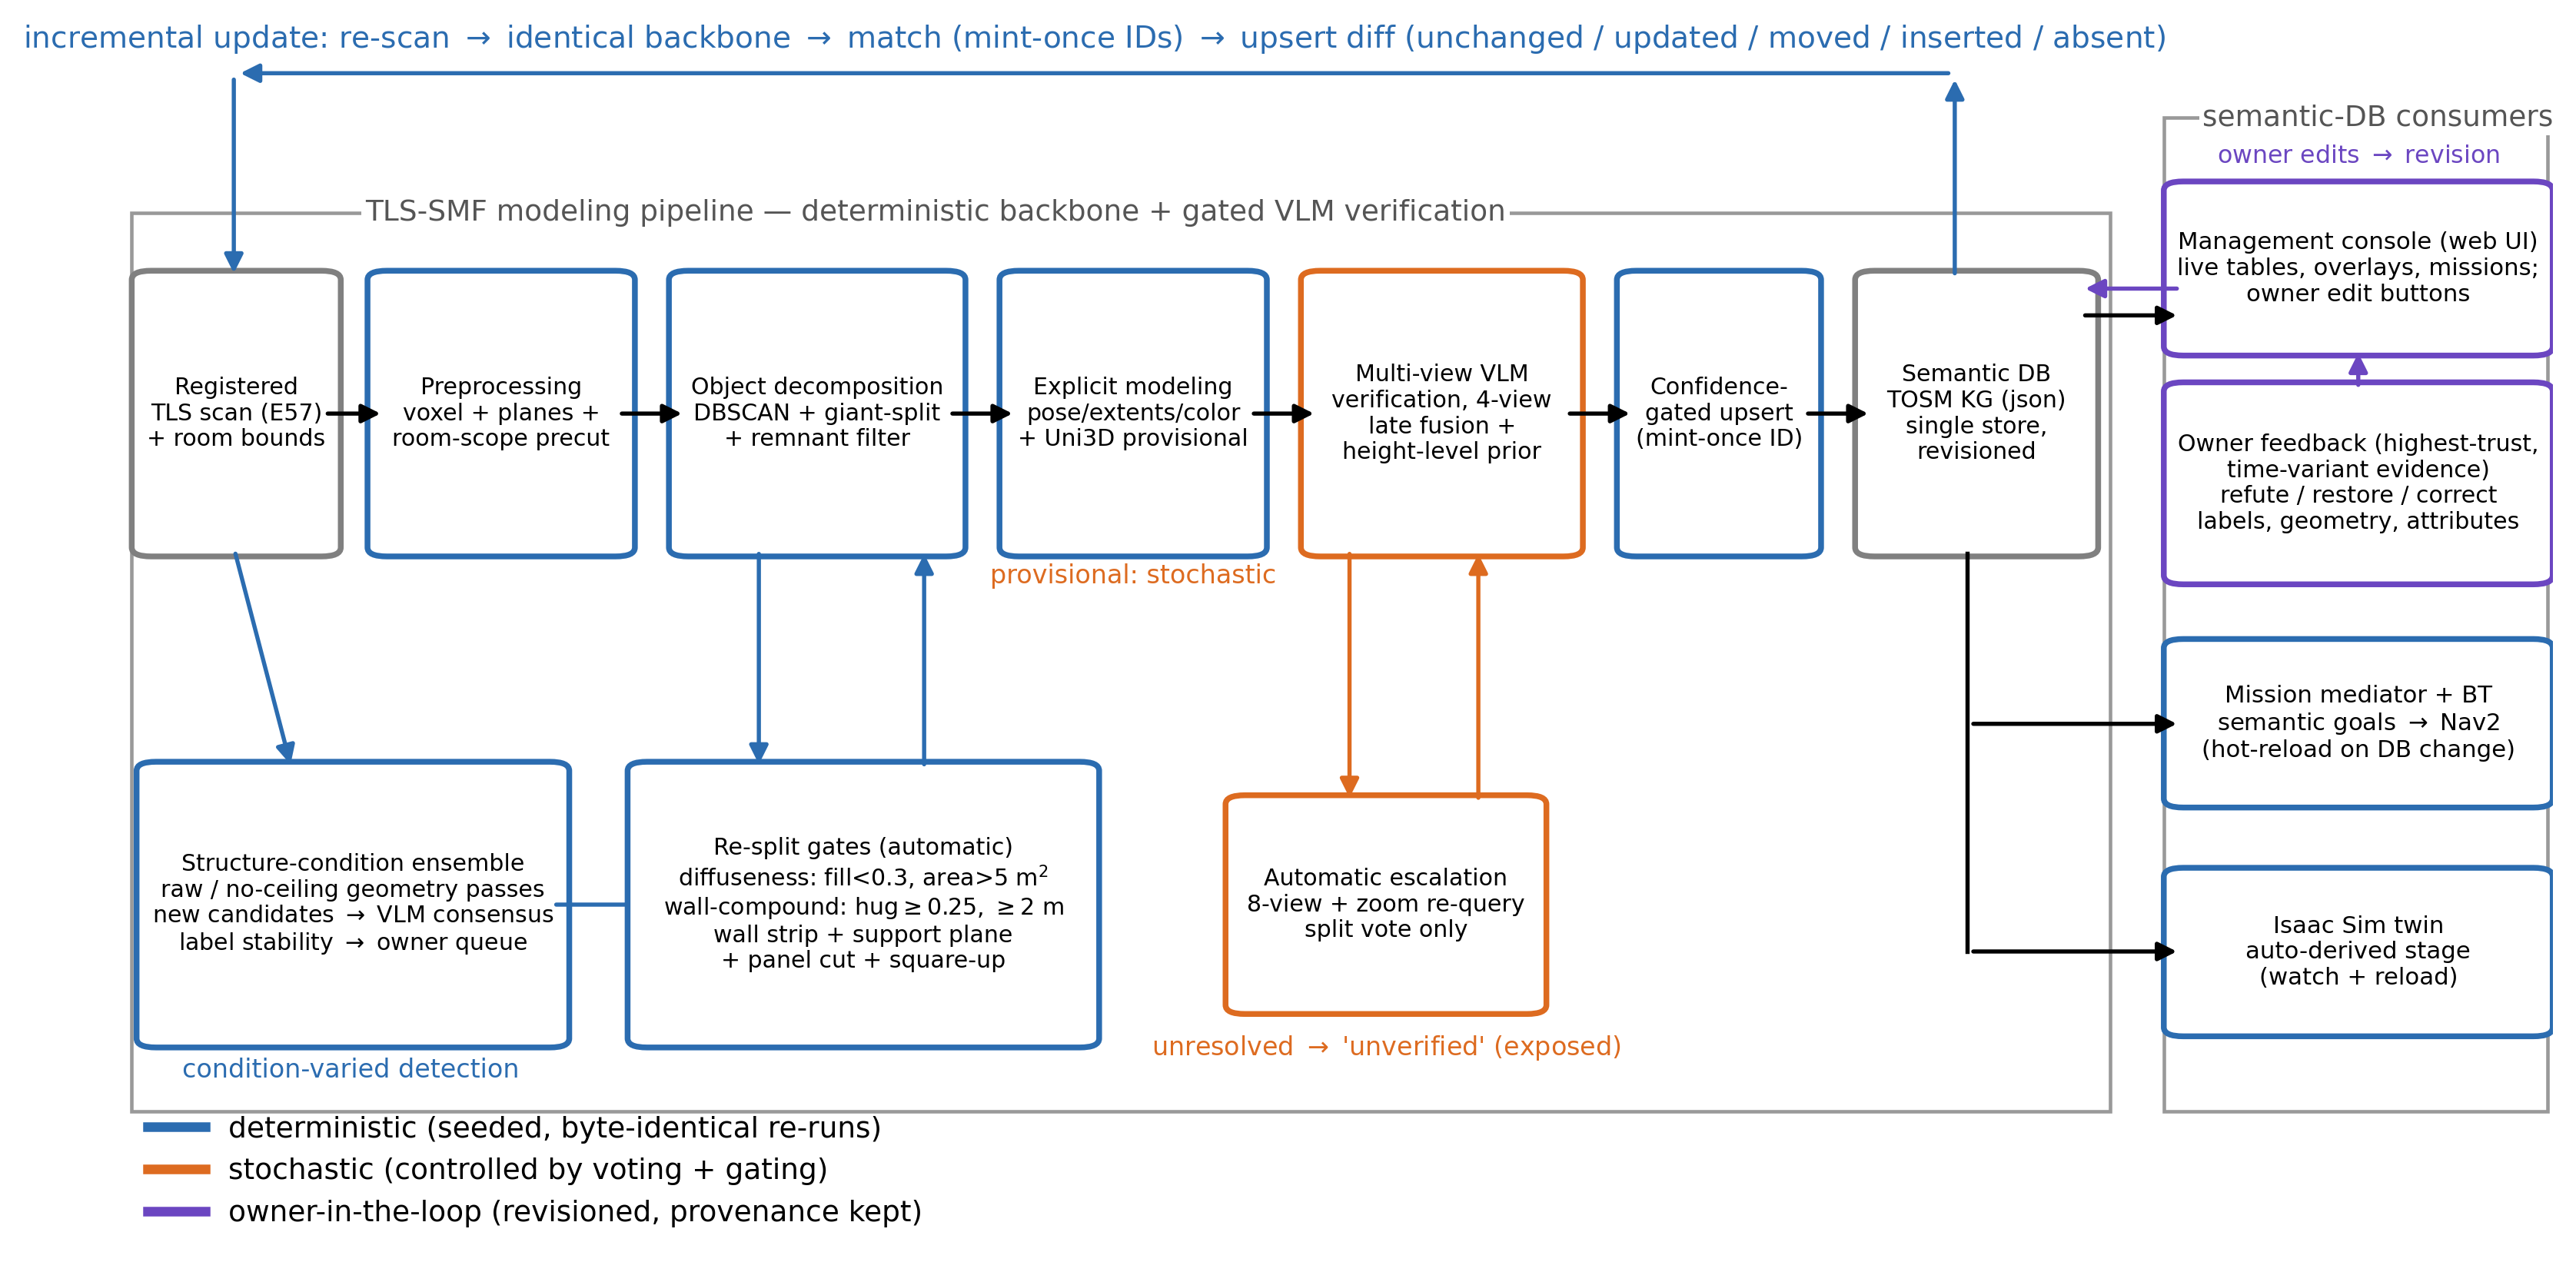
\includegraphics[width=0.95\linewidth]{figures/ele_fig1_architecture.png}
\caption{TLS-SMF architecture. Blue stages form the deterministic geometric
backbone (including the automatic re-split gates and the structure-condition
ensemble); orange stages are probabilistic semantic inference under voting,
escalation, and gating control; purple is the owner-in-the-loop revision path.
The knowledge graph is the single semantic store from which the console, the
mission mediator, and the simulation twin are derived. Four loops: escalation
(within verification), re-splitting (within decomposition), incremental update
(across scans), and owner feedback (across revisions).}
\label{fig:architecture}
\end{figure}

The color separation in the architecture is a claim boundary, not a drawing
convention. Everything in the backbone is seeded and parameter-fixed;
re-running it on the same host reproduces every retained cluster
byte-identically (Section~\ref{sec:exp-seg}). Everything downstream of the
first VLM call is stochastic; there the framework claims
\emph{control}---schema-forced outputs, multi-view voting, automatic
escalation, and confidence gating---rather than reproducibility. Each object
node carries the three TOSM description layers: a \emph{symbolic} model (type,
name, status), an \emph{explicit} model (pose, extents, yaw, color), and an
\emph{implicit} model (movability, openability, key-object status). Verified
and unverified content flows through the same graph but is separated at every
interface: verification status is part of the node schema, gating is applied
structurally at query time, and the place layer is derived from verified
objects only. The framework is fully automated \emph{after registered TLS
input}: scanner operation and vendor multi-setup registration are manual;
everything from E57 to queryable graph---including escalation decisions and
update classification---runs without human intervention, and objects the
verifier cannot resolve remain explicitly \texttt{unverified} rather than
being resolved by hand. The base algorithms are deliberately standard and
claimed as integration: RANSAC, DBSCAN, PCA modeling, open-vocabulary 3D
classification, per-view VLM querying, and the TOSM schema follow prior work.
The new mechanisms are the control structures wrapped around them.

\section{Deterministic Geometric Backbone}
\label{sec:backbone}

The backbone comprises three stages---preprocessing, decomposition with
remnant filtering, and explicit modeling with provisional
classification---connected in series so that each stage produces the
representation required by the next (Figure~\ref{fig:pipeline}). Because the
survey-grade scanner already provides a colored 3D point cloud directly, the
entire backbone operates on the point cloud without synthesizing multi-view
imagery for segmentation, preserving metric accuracy end to end. Every random
draw is seeded, so a re-run on the same host reproduces every retained cluster
byte-identically; this property is what makes verification results carryable
and diffs meaningful and, under reproducible acquisition, lets verification
cost track detected content change.

\begin{figure}[!htb]
\centering
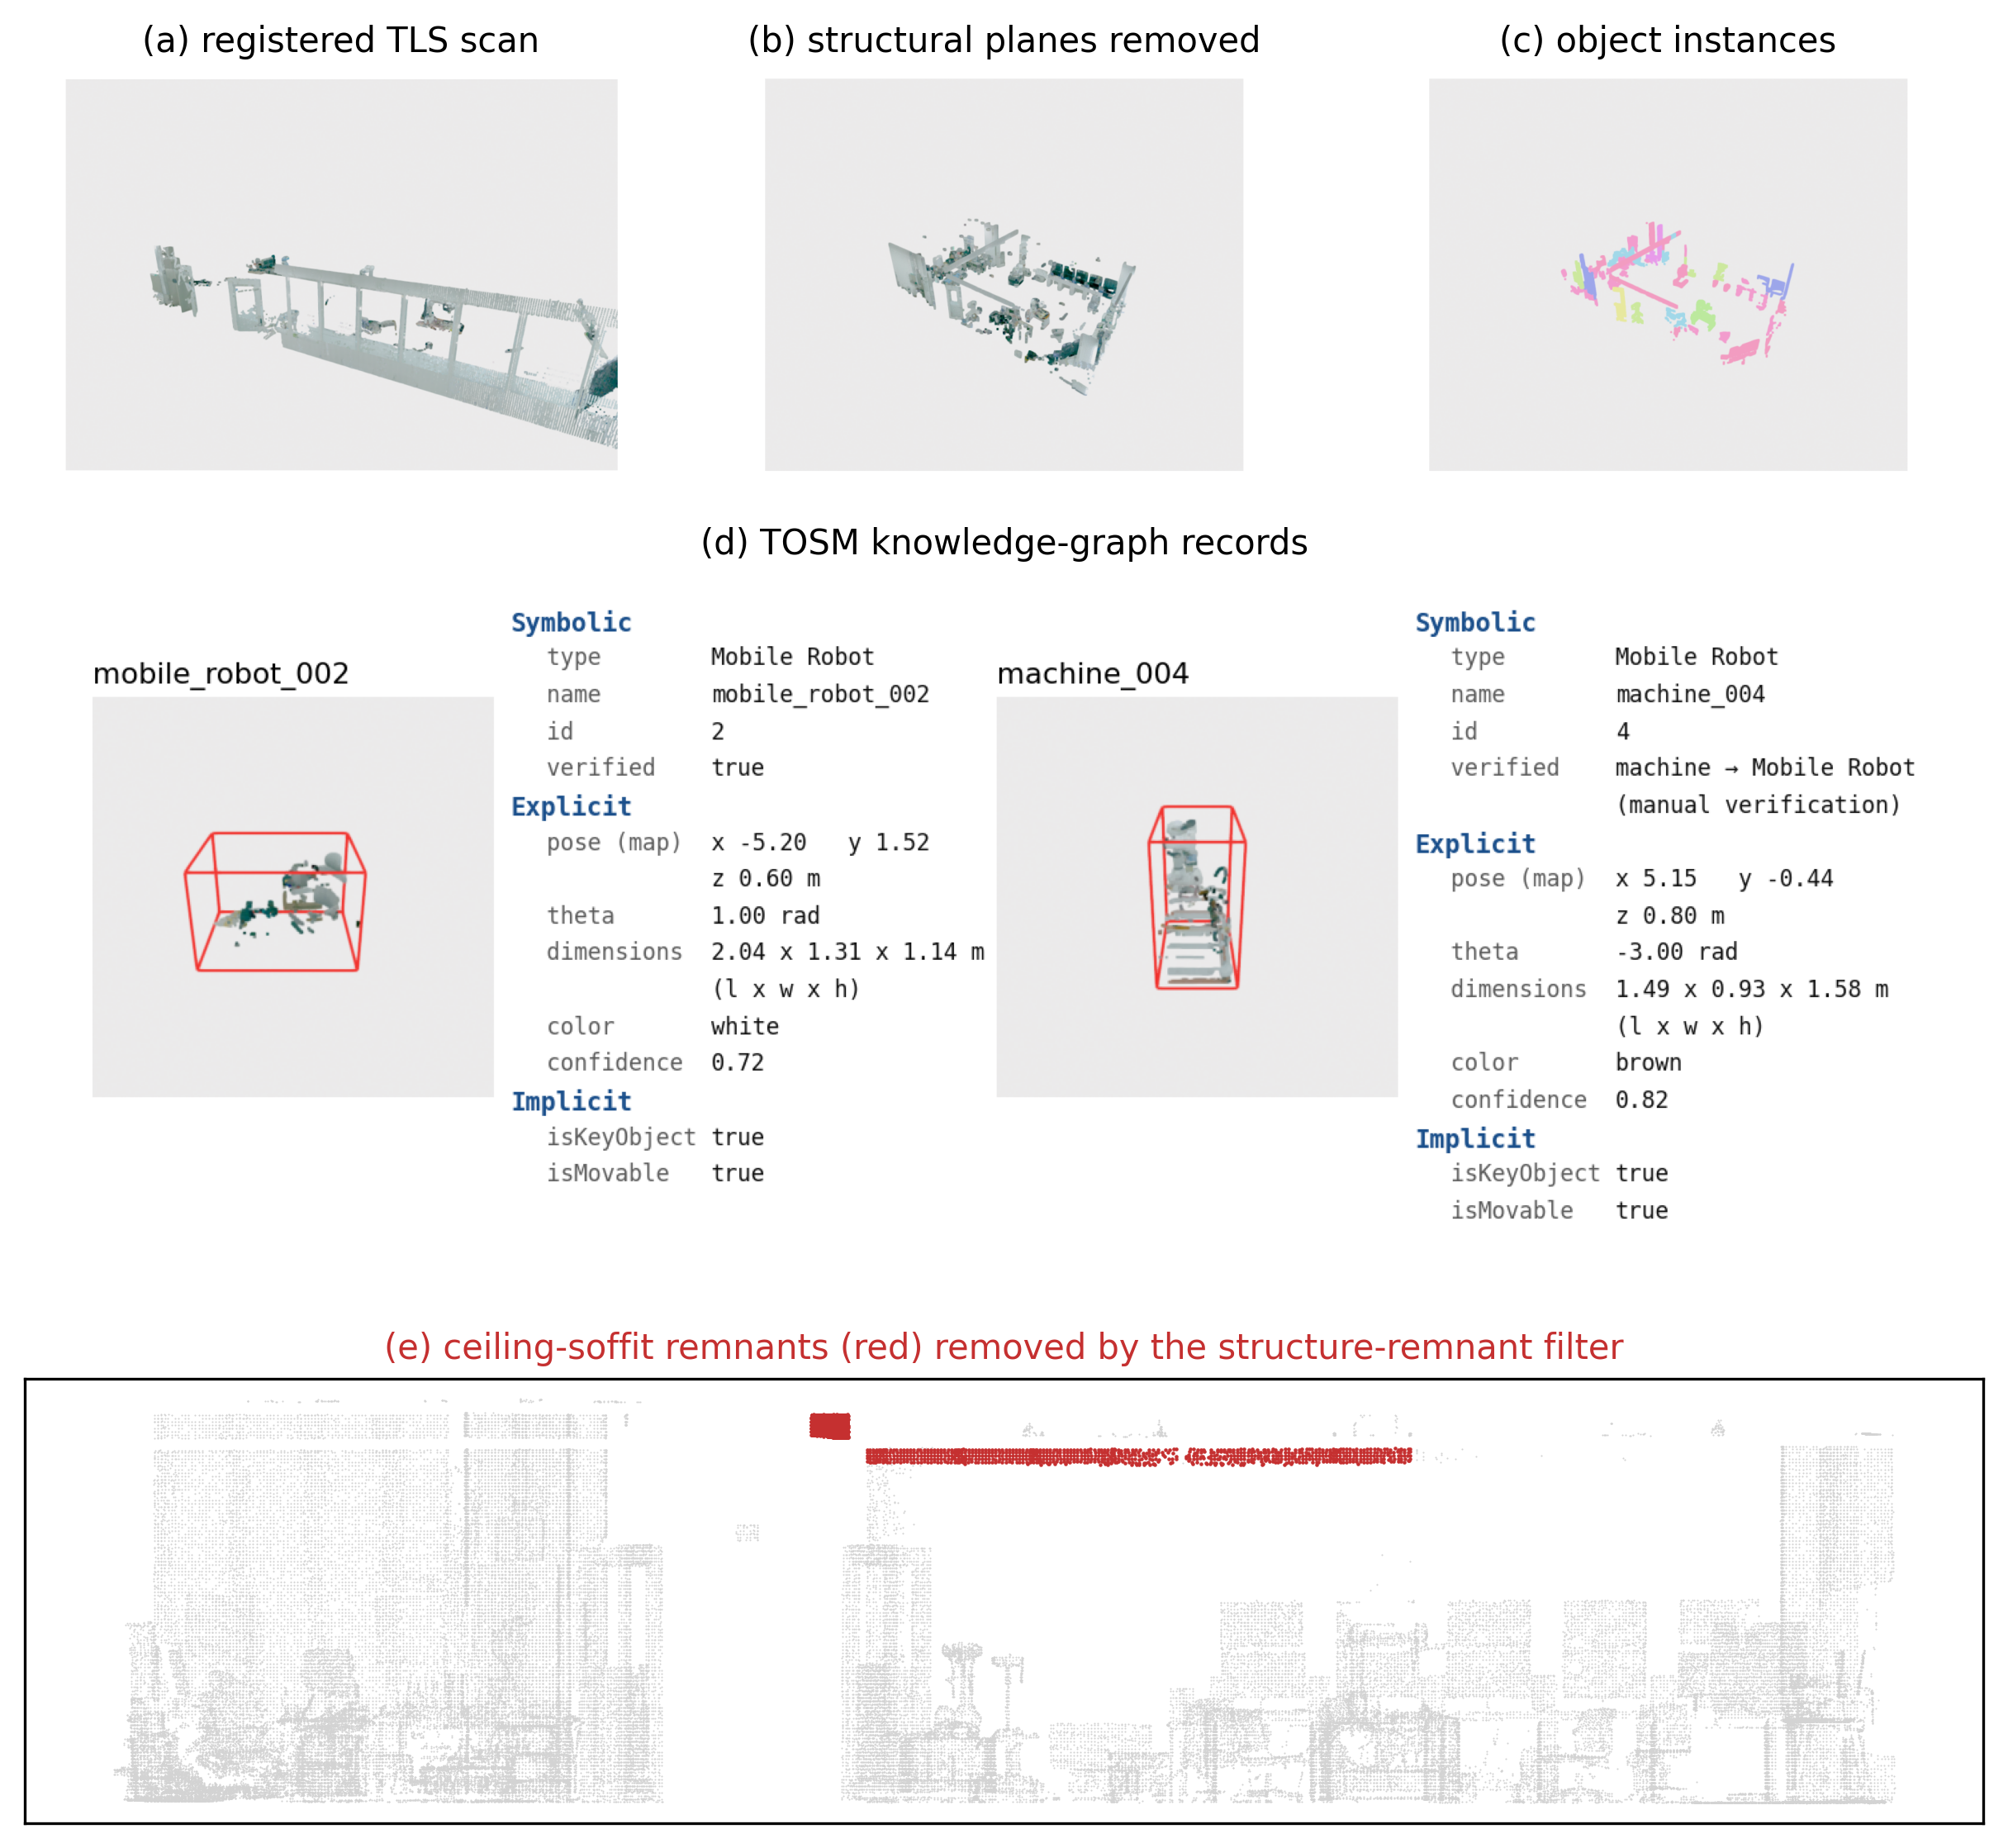
\includegraphics[width=0.92\linewidth]{figures/ele_fig2_pipeline.png}
\caption{Geometric backbone of TLS-SMF, illustrated on the test-room scene.
(a)~Registered multi-station TLS scan after preprocessing. (b)~The same cloud
after seeded-RANSAC removal of structural planes (floor, walls, ceiling).
(c)~Deterministic decomposition of the residual cloud into object instances;
identical inputs reproduce identical clusters with stable ordering. (d)~Two of
the resulting TOSM knowledge-graph records with their symbolic, explicit, and
implicit attributes. (e)~Structure-remnant filter, shown as a front elevation
of the showroom scene: the vertical soffit bands at the three-level ceiling
transitions (red) survive horizontal-plane removal and would otherwise surface
as phantom objects; the filter removes them while leaving every retained
cluster byte-identical.}
\label{fig:pipeline}
\end{figure}

\subsection{TLS Preprocessing and Structural-Plane Removal}
\label{subsec:preprocess}

The input is a registered E57 point cloud from the survey-grade scanner. When
the export contains multiple setups, the loader applies each setup's registered
pose and merges them into a single cloud; a 70M-point six-setup scan and a
pre-merged single-scan export are treated identically. The cloud is
voxel-downsampled at 3~cm---dense enough to retain object detail while bounding
the cost of all later stages---and kept in the scanner's registered frame; no
global normalization is applied. The floor height is estimated where a stage
needs it, by a robust statistic suited to that stage's input.

Structural surfaces---floor, walls, and ceiling---are then removed by
iterative RANSAC plane extraction~\cite{fischler1981ransac}. Each round draws
300 seeded random point triples, keeps the candidate with the most inliers at a
5~cm distance threshold, and refits it once by a least-squares (SVD) fit to
those inliers. A plane is removed only if it is structural by orientation:
near-horizontal ($|n_z|\ge0.85$; floors, ceilings, split ceiling levels) or
near-vertical ($|n_z|\le0.2$; walls). Interior slanted planes, which may belong
to furniture or fixtures, are preserved. The loop stops at the first of four
conditions: ten planes have been removed, fewer than 2{,}000 points remain, the
best remaining plane supports less than 4\% of the points still present, or the
best remaining plane is slanted ($0.2<|n_z|<0.85$), so that removing it would
begin carving objects. The fixed seed makes the extraction deterministic; the
pre-removal cloud is retained as a \emph{ceiling reference} for the remnant
filter below and for incremental re-runs.

\subsection{Geometric Object Decomposition and Structure-Remnant Filtering}
\label{subsec:decomposition}

The structure-free cloud is partitioned into object candidates by
fixed-parameter DBSCAN~\cite{ester1996dbscan} ($\varepsilon=0.30$~m, 100-point
minimum), followed by a \emph{conservative giant-split}: any cluster whose
horizontal footprint exceeds 2.5~m is re-clustered at a tighter
$\varepsilon=0.20$~m, and the split is accepted only if it yields at least two
sub-clusters of 100+ points---separating merged neighbors without shattering
genuinely large equipment. This stage is positioned deliberately: it is not a
novel segmentation algorithm but a \emph{reproducible decomposition designed
for verification and incremental diffing}. The requirement that motivates a
geometric, class-agnostic decomposition is that industrial and indoor
environments frequently contain fixtures, racks, and special equipment outside
the distribution of common training datasets, so segmentation bound to a
closed category set tends to miss unregistered objects or merge them
incorrectly; Section~\ref{subsec:exp-backbone} grounds this choice empirically
against learned alternatives.

\paragraph{Structure-remnant filter.}
Real buildings violate the implicit assumption that structure is planar and
objects are not. The showroom scene of Chapter~\ref{ch:experiments} has a
three-level ceiling ($z=2.48/2.18/1.95$~m): RANSAC removes each horizontal
ceiling plane, but the \emph{vertical soffit bands} at the level transitions
survive removal and surface as phantom objects
(Figure~\ref{fig:pipeline}e)---thin, wall-colored slabs that a downstream
verifier confidently misreads. The filter therefore removes any cluster that
passes all of the following tests, with thresholds fixed once and used
unchanged on every scene: (i)~soffit-scale geometry, i.e., a vertical extent
of at most 0.6~m with the bottom at least 1.5~m above the floor; (ii)~a thin
vertical planar band, i.e., a best-fit plane
with $|n_z|\le0.25$ and an RMS off-plane thickness of at most 3~cm;
(iii)~ceiling above, i.e., the footprint padded by 0.3~m contains at least 40
pre-removal points in the band from 2~cm to 45~cm above the cluster top;
(iv)~a dense horizontal layer, i.e., at least 60\% of those points concentrate
in a single $\sim$7~cm slab; and (v)~a topmost layer, i.e., the region above
that slab holds at most 20\% as many points as the slab itself, so that window
sills and wall remnants fail because the wall continues above them. Horizontal
and sloped ceiling patches are out of the filter's scope; the hybrid grid-map
structure filter of Section~\ref{sec:corrective} addresses the remaining wall,
ceiling, and outside-boundary remnants.

\subsection{Explicit Modeling and Provisional Classification}
\label{subsec:explicit}

Each cluster is summarized by an explicit model: axis extents and centroid,
yaw from the principal component of the horizontal point distribution, dominant
color, and point count. The position in the global frame is taken as the
bounding-box center and the size as the yaw-aligned extents (length, width,
height). These attributes are deterministic functions of the cluster; the
backbone's determinism claim covers geometry and these explicit attributes
only. A provisional semantic label is then attached by open-vocabulary
classification over a 30-class industrial vocabulary: the object points are
normalized and centered on a unit sphere, encoded by a point-cloud-direct
vision--language representation (Uni3D~\cite{zhou2024uni3d}), and labeled by
cosine similarity against text embeddings of the candidate categories. The
provisional label is explicitly \emph{not trusted}: the vocabulary ablation of
Section~\ref{sec:exp-ablation} shows that narrowing the vocabulary to the
deployment domain \emph{reduces} accuracy, indicating an embedding-level domain
gap rather than a class-list problem. The provisional label serves only as VLM
context and as a fallback name; every label a robot may act on must pass the
verification stage below. For each object the backbone also exports four
azimuth renders ($0/90/180/270^{\circ}$, elevation $25^{\circ}$, $512\times512$
pixels, with the 3D bounding box drawn in red), which are the input to
verification.

\section{Multi-View VLM Verification with Automatic Escalation}
\label{sec:verification}

\subsection{Schema-Forced Per-View Classification}
\label{subsec:prompts}

Verification submits each rendered view independently to a vision--language
model under a forced tool-use schema: the model must answer by calling a
declared JSON tool, so every response is schema-valid by construction and no
separate parsing or regular-expression post-processing is needed. Two prompts
are used (Figure~\ref{fig:prompt}). \emph{Prompt~1 (symbolic)}, once per
view, shows the model one render, the measured dimensions, the provisional
class, and an optional operator-supplied scene-level candidate vocabulary. The
decision rule is three-way: keep a correct label; if wrong, prefer a fitting
candidate; else emit an open-vocabulary common-noun label. Guardrails address
the failure modes of sparse point renders: measured dimensions are a hard
constraint, an oversize cluster is treated as merged objects (label the
dominant structure or \texttt{clutter}), no parts may be claimed that are not
outlined by points, thin flat objects are disambiguated among keyboard,
display, and shelf and never labeled as a ladder, and a chair requires a
visible seat pan of 0.3--0.6~m plus a backrest. The model returns a type, a
confidence, and a stated reason. \emph{Prompt~2 (implicit)}, once per object,
receives the fused type and the views and reports the TOSM implicit model:
\texttt{isKeyObject} (a fixed, distinctive landmark useful for localization),
\texttt{isMovable} (physically displaceable during normal operation), and, for
doors only, \texttt{isOpen} and \texttt{canBeOpen}. The geometric information
is provided only as context and is never modified by the model. Prompts,
decoding parameters, and the model version are recorded with every result; the
verifier model itself is a swappable component, and
Section~\ref{sec:exp-ablation} repeats the identical protocol across five
commercial VLMs.

\begin{figure}[!htb]
\centering
\fbox{\begin{minipage}{0.94\textwidth}\small
\textbf{P1 system (condensed).} Verifier for an indoor mobile robot. Input:
ONE render of a segmented 3D object (sparse laser points, red 3D box), its
classifier label \texttt{uni3d\_type}, optional candidates.
\emph{Decision rule:} (1)~KEEP a correct \texttt{uni3d\_type}; (2)~else
replace---prefer a fitting candidate, otherwise the most accurate common-noun
label; never `unknown'. \emph{Size sanity:} measured dimensions are a HARD
constraint; an oversize cluster is merged objects---label the dominant
structure or `clutter'. \emph{Sparse-render caution:} never claim parts not
outlined by points. \emph{Panel rule:} thin flat objects are keyboard /
display / shelf---never ladder. \emph{Chair gate:} visible seat pan
0.3--0.6~m plus backrest. If uncertain, keep a size-compatible label. Answer
ONLY via \texttt{report\_symbolic}.\\[2pt]
\textbf{P2 system (condensed).} From views and confirmed type, report
\texttt{isKeyObject} (fixed, distinctive landmark), \texttt{isMovable},
\texttt{isOpen}/\texttt{canBeOpen} (doors only, else null) ONLY via
\texttt{report\_implicit}.
\end{minipage}}
\caption{Condensed verification prompt design. Forced tool-use makes every
response schema-valid JSON; measured geometry is read-only context.}
\label{fig:prompt}
\end{figure}

\subsection{Confidence-Weighted Late Fusion}
\label{subsec:fusion}

The obvious multi-view strategy---feeding all views into one prompt
(\emph{early fusion})---\emph{degrades} accuracy on sparse point renders:
extra oblique speckle views invite over-confident misreadings that contaminate
the joint judgment (Section~\ref{subsec:exp-multiview}). Per-view votes are
therefore combined by confidence-weighted \emph{late fusion}, the analogue of
MVCNN-style aggregation~\cite{su2015mvcnn}. Let view $v$ return label $\ell_v$
(lowercased; no synonym mapping is applied at fusion time) with confidence
$c_v\in[0,1]$. Each candidate label accumulates the sum of the confidences of
the views that voted for it,
\begin{equation}
  s(\ell)=\sum_{v:\,\ell_v=\ell}c_v, \qquad
  \hat{\ell}=\arg\max_{\ell}s(\ell), \qquad
  \sigma=\frac{s(\hat{\ell})}{\sum_{\ell}s(\ell)},
  \label{eq:fusion}
\end{equation}
where $\hat{\ell}$ is the fused type and $\sigma$ its \emph{vote share}. A
confidence-weighted sum, rather than a view count, lets one hesitant dissenter
matter less than a confident one; a single contaminated view is simply outvoted.
The per-view votes are stored in the record, so a downstream consumer can
distinguish a 4/4 unanimous label from a 2/4 split---a free uncertainty
signal.

\subsection{Automatic Escalation and Verification Tiers}
\label{subsec:escalation}

Three outcomes follow (Figure~\ref{fig:escalation}). If the four votes are
unanimous, the object is \texttt{verified}; unanimity is empirically a strong
signal (94--100\% precision against confirmed ground truth on the industrial
scenes, Section~\ref{sec:exp-verify}), although its failure modes are
documented there as well. If the vote splits, the object \emph{escalates
automatically}: eight additional images---four diagonal azimuths and four
zoomed close-ups---are classified, and the fusion is recomputed over all twelve
votes pooled. If the post-escalation share reaches $\sigma\ge0.6$ the object
becomes \texttt{verified\_escalated}; otherwise it remains
\texttt{unverified}. The 0.6 threshold was fixed a priori as the smallest round
value that demands a clear supermajority of the confidence mass; it gates
\emph{status only}, the fused label being recorded either way, and
Section~\ref{sec:exp-verify} re-scores the stored votes across a threshold
sweep to quantify the resulting precision--recall trade-off. Crucially,
unresolved objects are not hidden, discarded, or resolved by a human: they
stay in the graph with their failed candidate label attached, and the query
interface (Section~\ref{sec:query}) is responsible for making their status
impossible to ignore. Implicit robot-facing attributes are inferred once at
fusion time from the winning view set. Escalation bounds cost: only split
votes pay for the wider view set, and per-call cost is on the order of \$0.01,
so a scene verifies for a few dollars.

\begin{figure}[!htb]
\centering
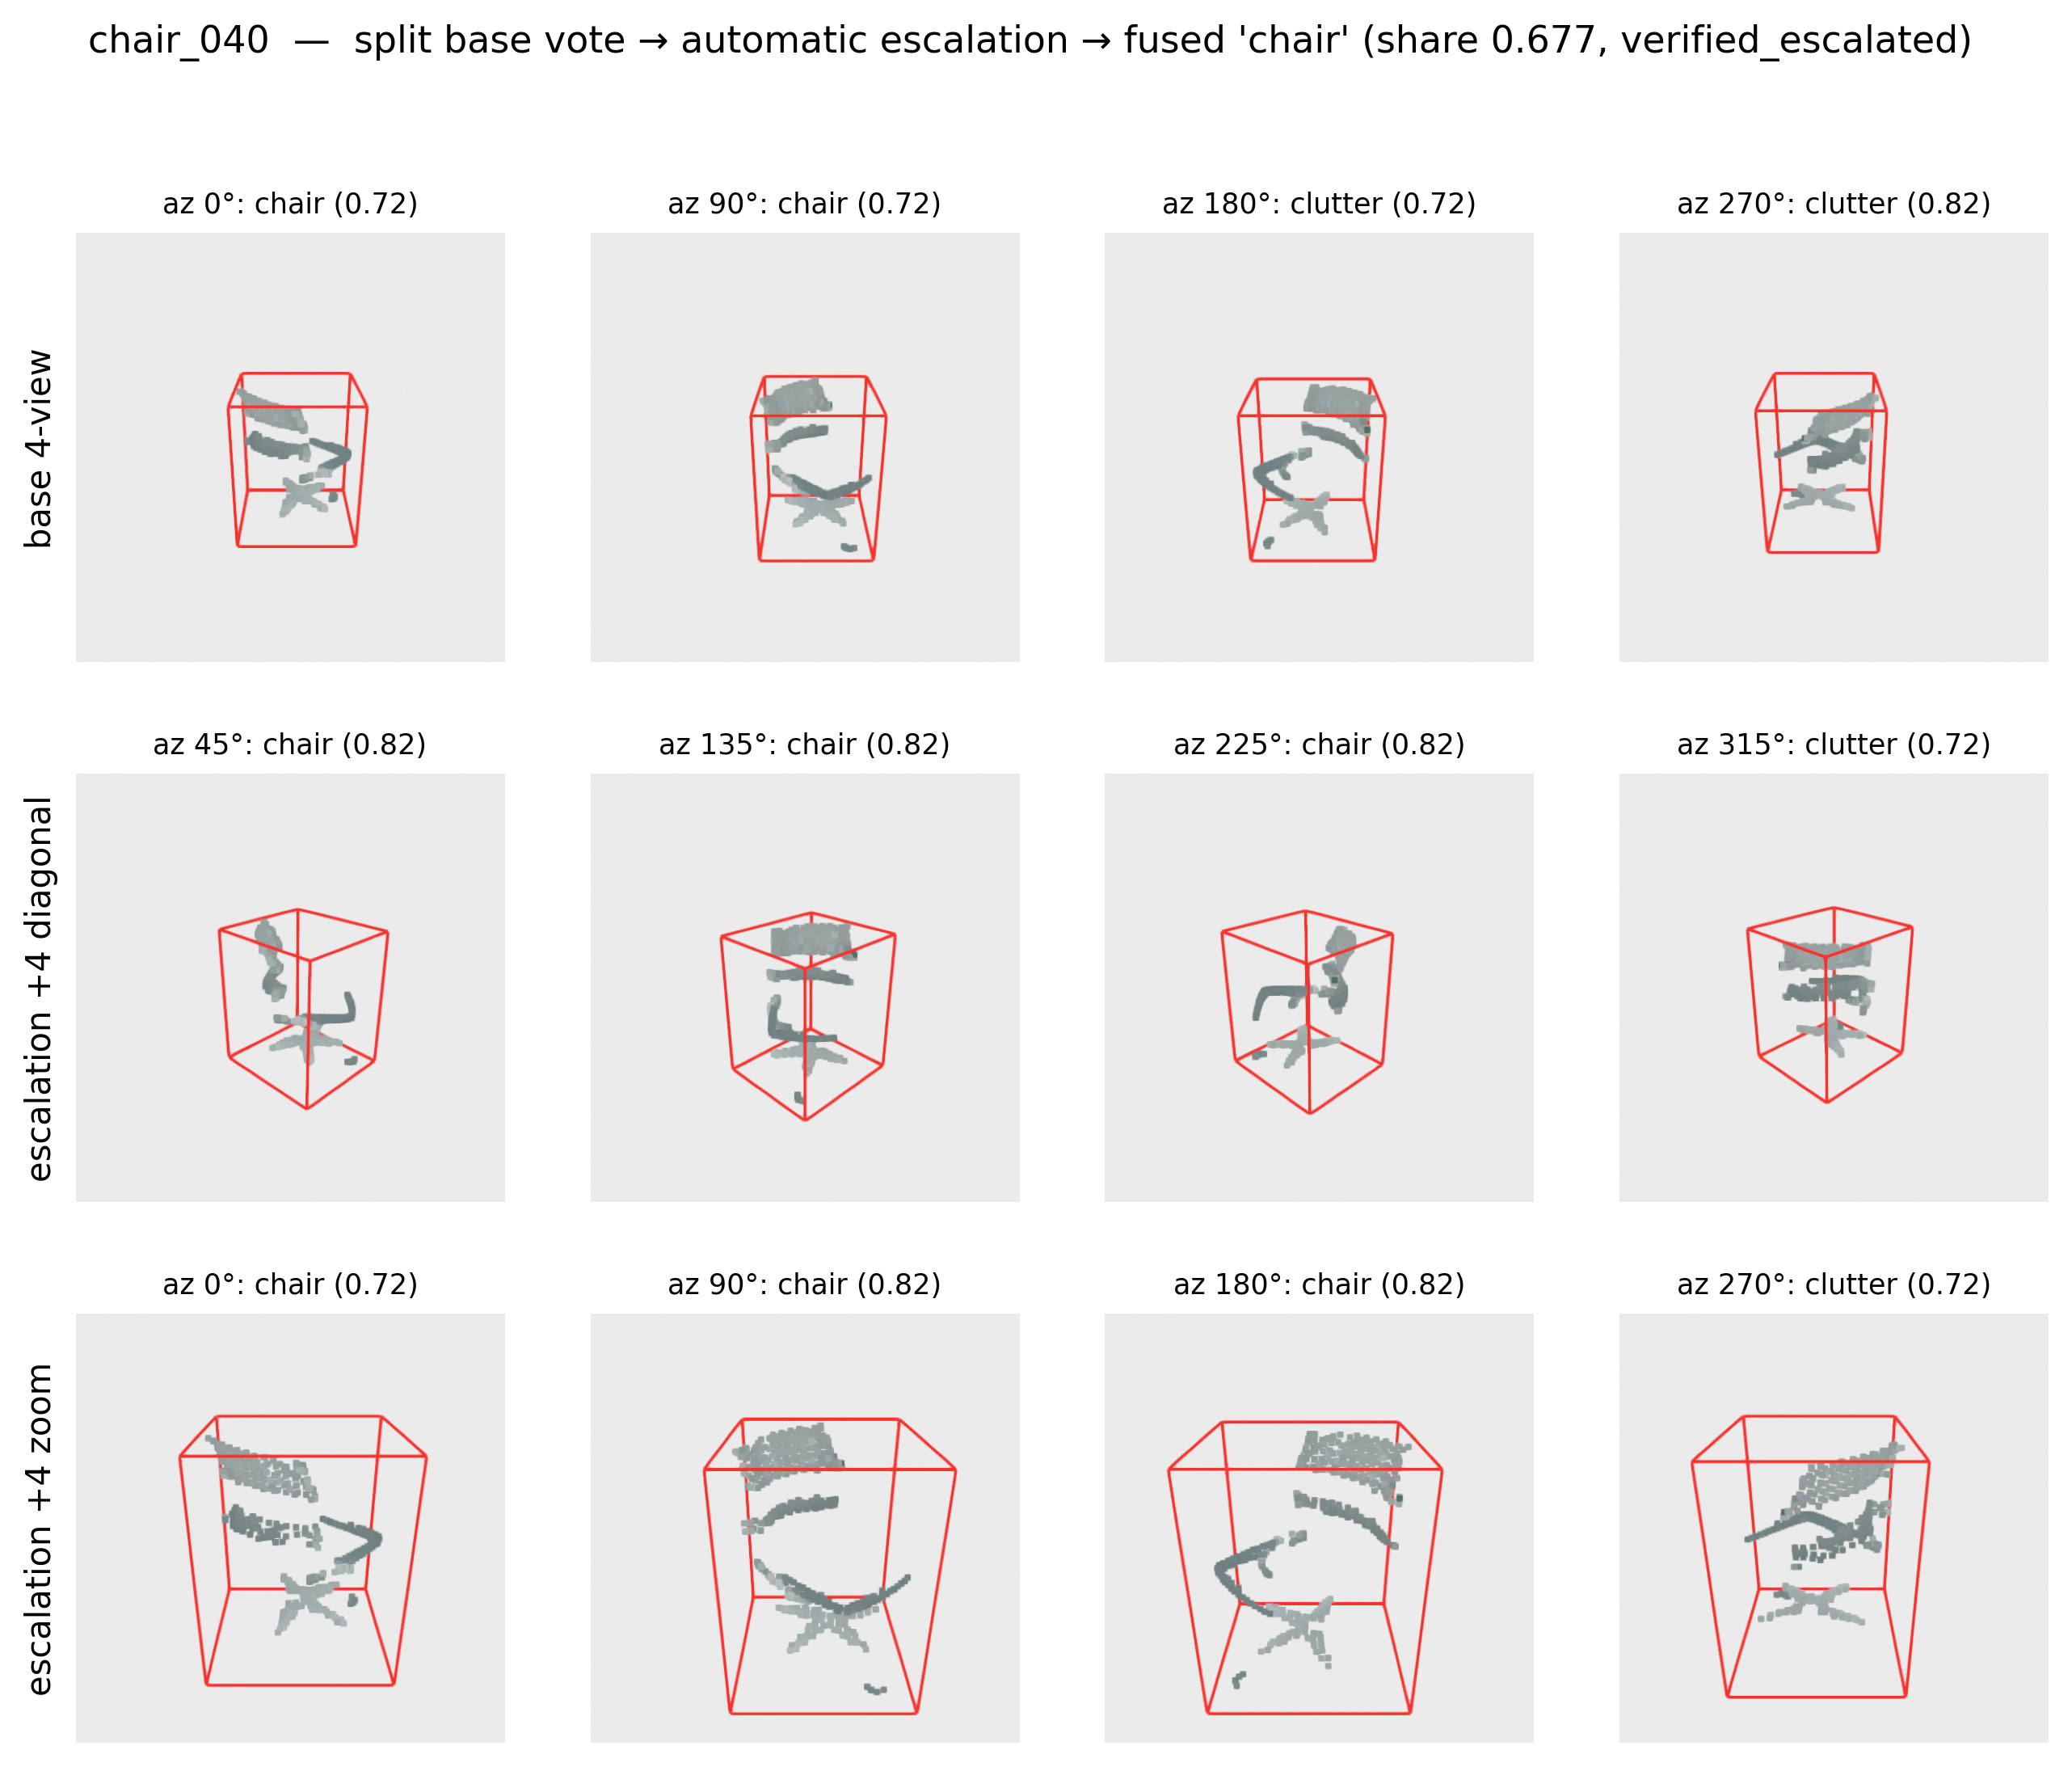
\includegraphics[width=0.95\linewidth]{figures/ele_fig3_multiview_escalation.png}
\caption{Multi-view verification and automatic escalation, with per-view
votes, fused share, and the three terminal statuses.}
\label{fig:escalation}
\end{figure}

\section{TOSM Schema and Serialization}
\label{sec:tosm-schema}

Recognized objects and places are represented in the three layers of TOSM.
Environmental elements are classified into Object and Place, subclasses of the
top-level class EnvironmentalElement, and each element carries datatype
properties corresponding to the Symbolic, Explicit, and Implicit layers as well
as object properties expressing spatial relations among elements.
Table~\ref{tab:tosm-object} defines the datatype properties of an Object and
Table~\ref{tab:tosm-place} those of a Place; Table~\ref{tab:predicates} lists
the object properties. Identifiers and categories are placed in the Symbolic
layer, scanner-measured pose, size, and color in the Explicit layer, and
information derived from inference---key-object indication, movability, door
state, place purpose---in the Implicit layer. Beyond the lineage's schema, each
node in this work carries a verification status drawn from the tier set
\begin{equation}
\begin{aligned}
\mathcal{T}=\{&\texttt{verified},\ \texttt{verified\_escalated},\ \texttt{verified\_recovery},\\
&\texttt{verified\_owner},\ \texttt{unverified},\ \texttt{refuted}\},
\end{aligned}
\label{eq:tiers}
\end{equation}
ordered by evidence source (unanimity, escalated supermajority,
agreement-gated recovery, and owner declaration at confidence 1.0), together
with provenance (per-view votes, fused share, escalation flag, model version),
a per-revision history, and \texttt{firstSeen}/\texttt{lastSeen} timestamps.

\begin{table}[htbp]
  \centering
  \caption{TOSM datatype properties for an Object. \texttt{isOpen} and
  \texttt{canBeOpen} have Door as their domain; the verification and provenance
  properties are additions of this work.}
  \label{tab:tosm-object}
  \begin{tabular}{l l l l}
    \toprule
    \textbf{Layer} & \textbf{Property} & \textbf{Domain} & \textbf{Range} \\
    \midrule
    \multirow{3}{*}{symbolicModel}
      & name & Object & string \\
      & ID   & Object & int \\
      & verificationStatus & Object & $\mathcal{T}$ (Equation~\ref{eq:tiers}) \\
    \midrule
    \multirow{5}{*}{explicitModel}
      & pose & Object & $(x, y, z, \theta)$ \\
      & coordinateFrame & Object & string \\
      & size & Object & $(l, w, h)$ \\
      & color & Object & string \\
      & heightLevel & Object & \{low, mid, high\} \\
    \midrule
    \multirow{5}{*}{implicitModel}
      & isKeyObject & Object & boolean \\
      & isMovable & Object & boolean \\
      & isOpen & Door & boolean \\
      & canBeOpen & Door & boolean \\
      & labelStability & Object & \{stable, unstable\} \\
    \bottomrule
  \end{tabular}
\end{table}

\begin{table}[htbp]
  \centering
  \caption{TOSM datatype properties for a Place, as instantiated by the
  object-grounded place layer of Section~\ref{sec:place}.}
  \label{tab:tosm-place}
  \begin{tabular}{l l l l}
    \toprule
    \textbf{Layer} & \textbf{Property} & \textbf{Domain} & \textbf{Range} \\
    \midrule
    \multirow{2}{*}{symbolicModel}
      & name & Place & string (LLM-derived from ring code) \\
      & ID   & Place & int \\
    \midrule
    \multirow{4}{*}{explicitModel}
      & boundary & Place & polygon (SLIC region) \\
      & position & Place & $(x, y, z)$ \\
      & areaTotal & Place & float \\
      & coordinateFrame & Place & string \\
    \midrule
    \multirow{3}{*}{implicitModel}
      & purpose & Place & string \\
      & keyObject & Place & Object ref \\
      & isAdjacentTo & Place & Place ref \\
    \bottomrule
  \end{tabular}
\end{table}

\begin{table}[htbp]
  \centering
  \caption{Spatial-relation object properties and the consistency rules
  enforced when they are recomputed at each upsert.}
  \label{tab:predicates}
  \begin{tabularx}{\textwidth}{l l X}
    \toprule
    \textbf{Predicate} & \textbf{Domain $\to$ Range} & \textbf{Rule enforced} \\
    \midrule
    isInsideOf & Object $\to$ Place & functional (anchor cell containment) \\
    isNextTo & Object $\to$ Object & symmetric; kept only within the same place \\
    isOn / isAboveOf & Object $\to$ Object & asymmetric; requires rotated-footprint overlap \\
    isAdjacentTo & Place $\to$ Place & symmetric \\
    isKeyObjectOf & Object $\to$ Place & functional; refuted objects excluded \\
    isMovable / isStatic & Object $\to$ bool & mutually exclusive \\
    \bottomrule
  \end{tabularx}
\end{table}

Instead of the OWL representation used by prior work, the graph is serialized
in a VDA~5050-based JSON format~\cite{vda5050} for compatibility with downstream
robot-operation standards, and exported in parallel as map-scoped Neo4j Cypher
so that multiple sites and epochs coexist in one database. VDA~5050 specifies
the communication between automated guided vehicles and a master control; this
work borrows its message schema to express each semantic object as a JSON
record composed of header metadata (manufacturer, serial number, timestamp,
version) and an object array, so that the semantic model can be consumed by an
AGV control pipeline without a separate conversion step. TOSM fields with no
standard slot travel in the extensible \texttt{properties} map, so consumers
that only know the base schema can still read the message
(Table~\ref{tab:mapping}); Code~\ref{code:record} shows an example record.

\begin{table}[htbp]
  \centering
  \caption{TOSM $\to$ VDA~5050-style JSON field mapping.}
  \label{tab:mapping}
  \begin{tabularx}{\textwidth}{l l X}
    \toprule
    \textbf{TOSM model} & \textbf{Element} & \textbf{JSON field} \\
    \midrule
    symbolic & class & \texttt{type} \\
             & name / identity & \texttt{name}, \texttt{id} \\
             & verification status & \texttt{properties.verificationStatus} \\
    explicit & position, height & \texttt{poseX}, \texttt{poseY}, \texttt{properties.poseZ} \\
             & orientation, size & \texttt{poseTheta}, \texttt{dimensions\{l,w,h\}} \\
             & color & \texttt{color} \\
    implicit & landmark / movability & \texttt{properties.isKeyObject}, \texttt{isMovable} \\
             & door state & \texttt{properties.isOpen}, \texttt{canBeOpen} \\
    --       & VLM audit trail & \texttt{properties.viewVotes}, \texttt{symbolicReason}, \texttt{confidence} \\
    \bottomrule
  \end{tabularx}
\end{table}

\begin{quote}
\small\ttfamily
\begin{verbatim}
{
  "manufacturer": "CASELAB", "serialNumber": "...", "version": "0.0.0",
  "semanticObjects": [
    {
      "type": "control panel", "id": "0", "name": "control_panel_000",
      "poseX": 6.49, "poseY": 4.11, "poseTheta": -3.12,
      "dimensions": { "length": 5.75, "width": 0.71, "height": 3.24 },
      "color": "brown", "confidence": 1.0,
      "properties": {
        "poseZ": 0.63, "coordinateFrame": "map", "source": "DBSCAN+Uni3D",
        "verificationStatus": "verified", "viewVotes": [...],
        "isKeyObject": true, "isMovable": false,
        "isOpen": null, "canBeOpen": null,
        "symbolicReason": "...",  "implicitReason": "..."
      }
    }
  ]
}
\end{verbatim}
\end{quote}
\noindent\textbf{Code 4.1.}\quad Example of a semantic-object JSON record
(VDA~5050 message format; some values abbreviated).
\label{code:record}
\medskip

\section{Object Identity Matching}
\label{sec:matching}

The update problem is an \emph{identity} problem before it is a geometry
problem: a robot that plans against node IDs needs yesterday's chair to be
today's chair. The policy is \textbf{mint-once}: a node ID is minted when an
object first enters the graph---derived from a fingerprint of its birth-time
anchor (map, position, extent)---and never changes afterwards. The fingerprint
is a candidate-retrieval key, not the identity itself; after minting, matching
alone carries identity forward. Matching between a new scan's records and
existing nodes runs in two passes.

\begin{enumerate}
\item \textbf{Spatial pass.} A record matches a node if their 3D centroids
agree within 0.5~m and each of the three extents agrees within a per-axis
tolerance of $\max(0.3\cdot\max(d_{\mathrm{old}},d_{\mathrm{new}}),\,0.15\,\mathrm{m})$---a
30\% relative band with a 15~cm absolute floor so that small objects are not
over-constrained. No type constraint applies in this pass; a changed label on a
geometrically stable object is recorded as an update, not a new object. Matches
update pose and extents in place (\texttt{unchanged}/\texttt{updated}).
\item \textbf{Move pass.} Remaining records match remaining nodes of the
\emph{same type} with dimensions consistent under the same tolerance, within a
6~m horizontal search radius, producing \texttt{moved} nodes with preserved
IDs. Generic types (\texttt{clutter}, \texttt{unknown}) are excluded from this
pass: a generic label carries too little identity for displacement claims, and
the real two-epoch data showed that admitting them fabricates 2--5~m ``moves''
between unrelated piles.
\end{enumerate}

When several nodes satisfy the predicate for one record, the record claims the
node with the smallest horizontal centroid distance; when several records
compete for one node, the first claim wins and the node is removed from the
candidate pool. Assignment is therefore greedy in the backbone's deterministic
cluster order, so the assignment itself is reproducible. The thresholds encode
physical priors rather than tuned values: 0.5~m is below the smallest
inter-object spacing a scan-to-scan pose drift is expected to produce for a
stationary object and far above the $\le$5~cm registration residual; the
30\%/0.15~m extent band absorbs partial-view truncation without admitting
differently sized objects; and 6~m bounds a within-room relocation. Records
that match nothing are minted as new nodes (\texttt{inserted}); nodes that no
record claims are marked \texttt{absent} but retained with their full history,
so an object that returns later resumes its original identity. Formally, the
match function is
\begin{equation}
m(n,r)=\mathbb{1}[\lVert p_n-p_r\rVert_{3\mathrm{D}}\le0.5]\cdot
\prod_{k\in\{l,w,h\}}\mathbb{1}\bigl[\,|d_{n,k}-d_{r,k}|\le
\max(0.3\max(d_{n,k},d_{r,k}),0.15)\bigr],
\label{eq:match}
\end{equation}
with the move-pass variant substituting a 6~m horizontal bound and an
exact-type, non-generic constraint. The upsert decision for each record--node
pair follows the deterministic cascade \emph{match} $\rightarrow$ \emph{move}
$\rightarrow$ \emph{insert}, with unclaimed nodes marked \emph{absent}; every
transition appends to the node's history, and no node is ever deleted
(Figure~\ref{fig:upsert}).

\begin{figure}[!htb]
\centering
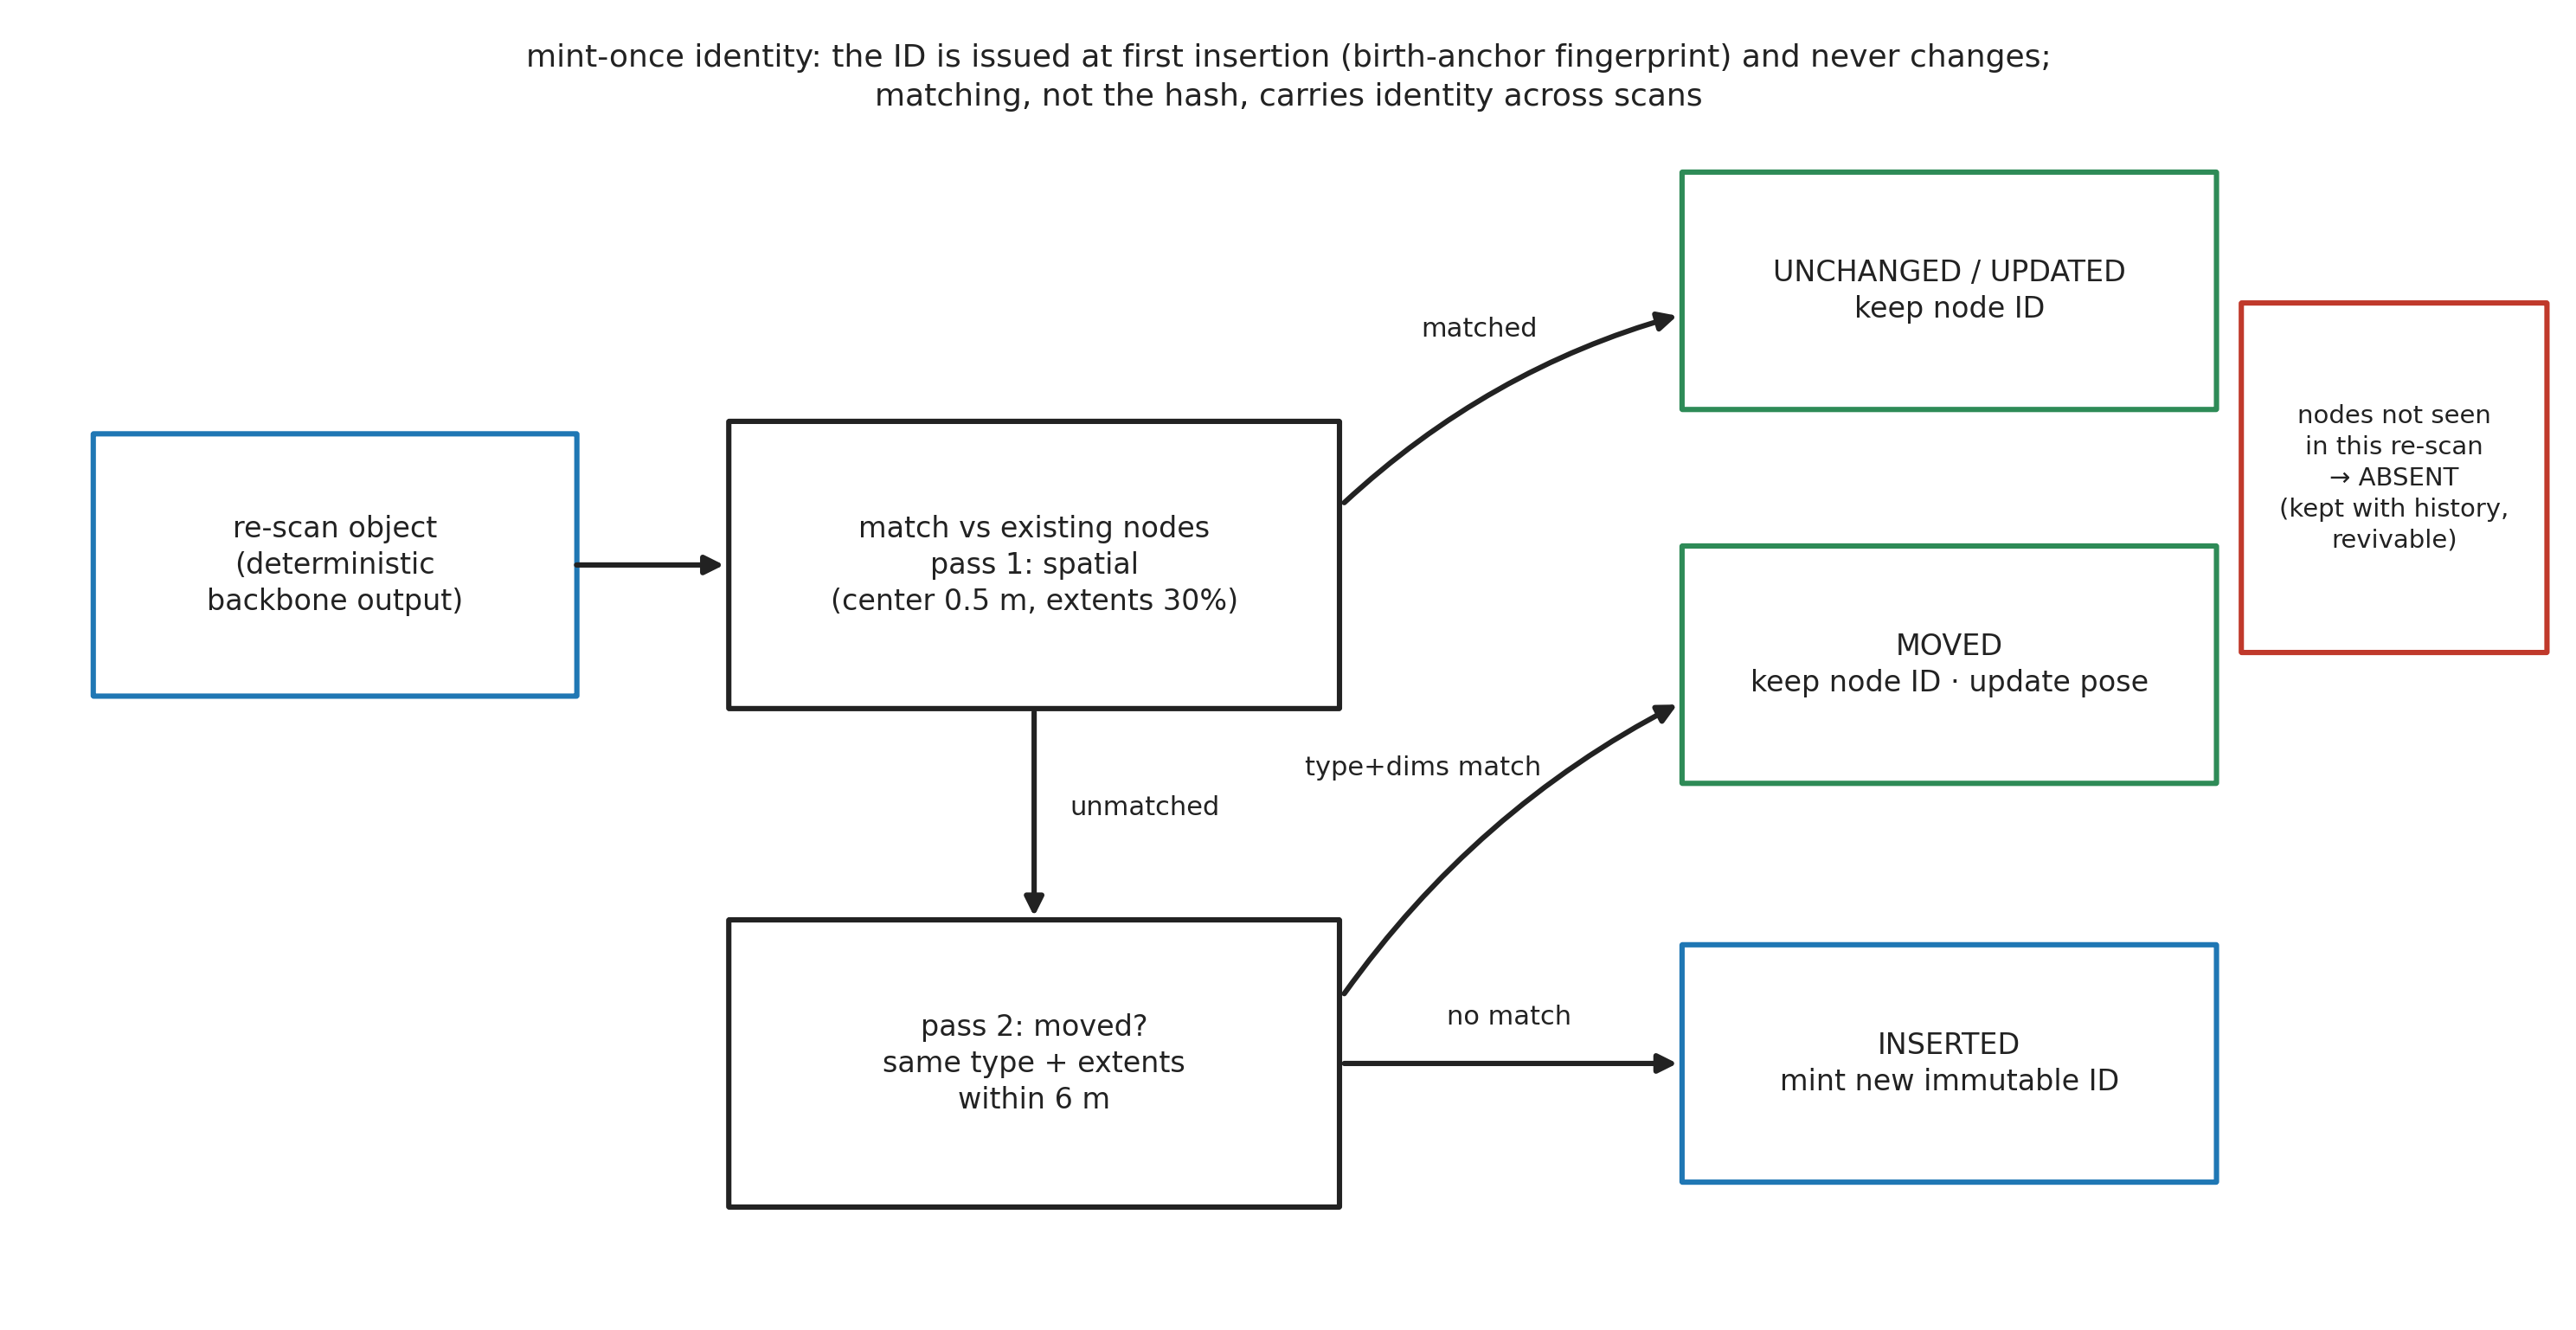
\includegraphics[width=0.9\linewidth]{figures/ele_fig5_identity_upsert.png}
\caption{Identity matching and confidence-gated upsert: mint-once IDs,
two-pass matching, and the five node outcomes across a re-scan.}
\label{fig:upsert}
\end{figure}

\section{Confidence-Gated Graph Upsert}
\label{sec:upsert}

Each scan epoch applies its matched record set to the knowledge graph as a
node-level upsert---no rebuild. Edges (spatial relations recomputed from
explicit models) are scoped to the map and revision and organized by the place
layer: \texttt{isNextTo} is kept only between objects of the same place
(proximity across a place boundary is expressed at the place level as
\texttt{isAdjacentTo}), vertical relations \texttt{isOn}/\texttt{isAboveOf}
must pass a rotated-footprint overlap test (a separating-axis check that
discards the long-range stacked relations oversized merged clusters otherwise
produce), and each place designates a key object (the VLM's implicit
\texttt{isKeyObject} among verified members, falling back to the most confident
specific-type verified member; objects refuted by owner feedback are excluded
from designation while remaining in the graph as annotated errors)
(Figure~\ref{fig:relmap}). Because unchanged objects reproduce byte-identical
clusters, their verification results are carried over by content hash and an
identical-input repeat scan costs \emph{zero} VLM calls; a changed scan of the
same acquisition quality pays only for changed clusters. The carry-over is
conditional on reproducible acquisition: when scan quality itself changes
between epochs, no cluster hashes match and the epoch pays full verification
cost (Section~\ref{sec:exp-update}). All numeric constants of
Sections~\ref{sec:backbone}--\ref{sec:upsert} were fixed on the development
epochs and applied unchanged to the later epoch and to the cross-floor scene.

\begin{figure}[!htb]
\centering
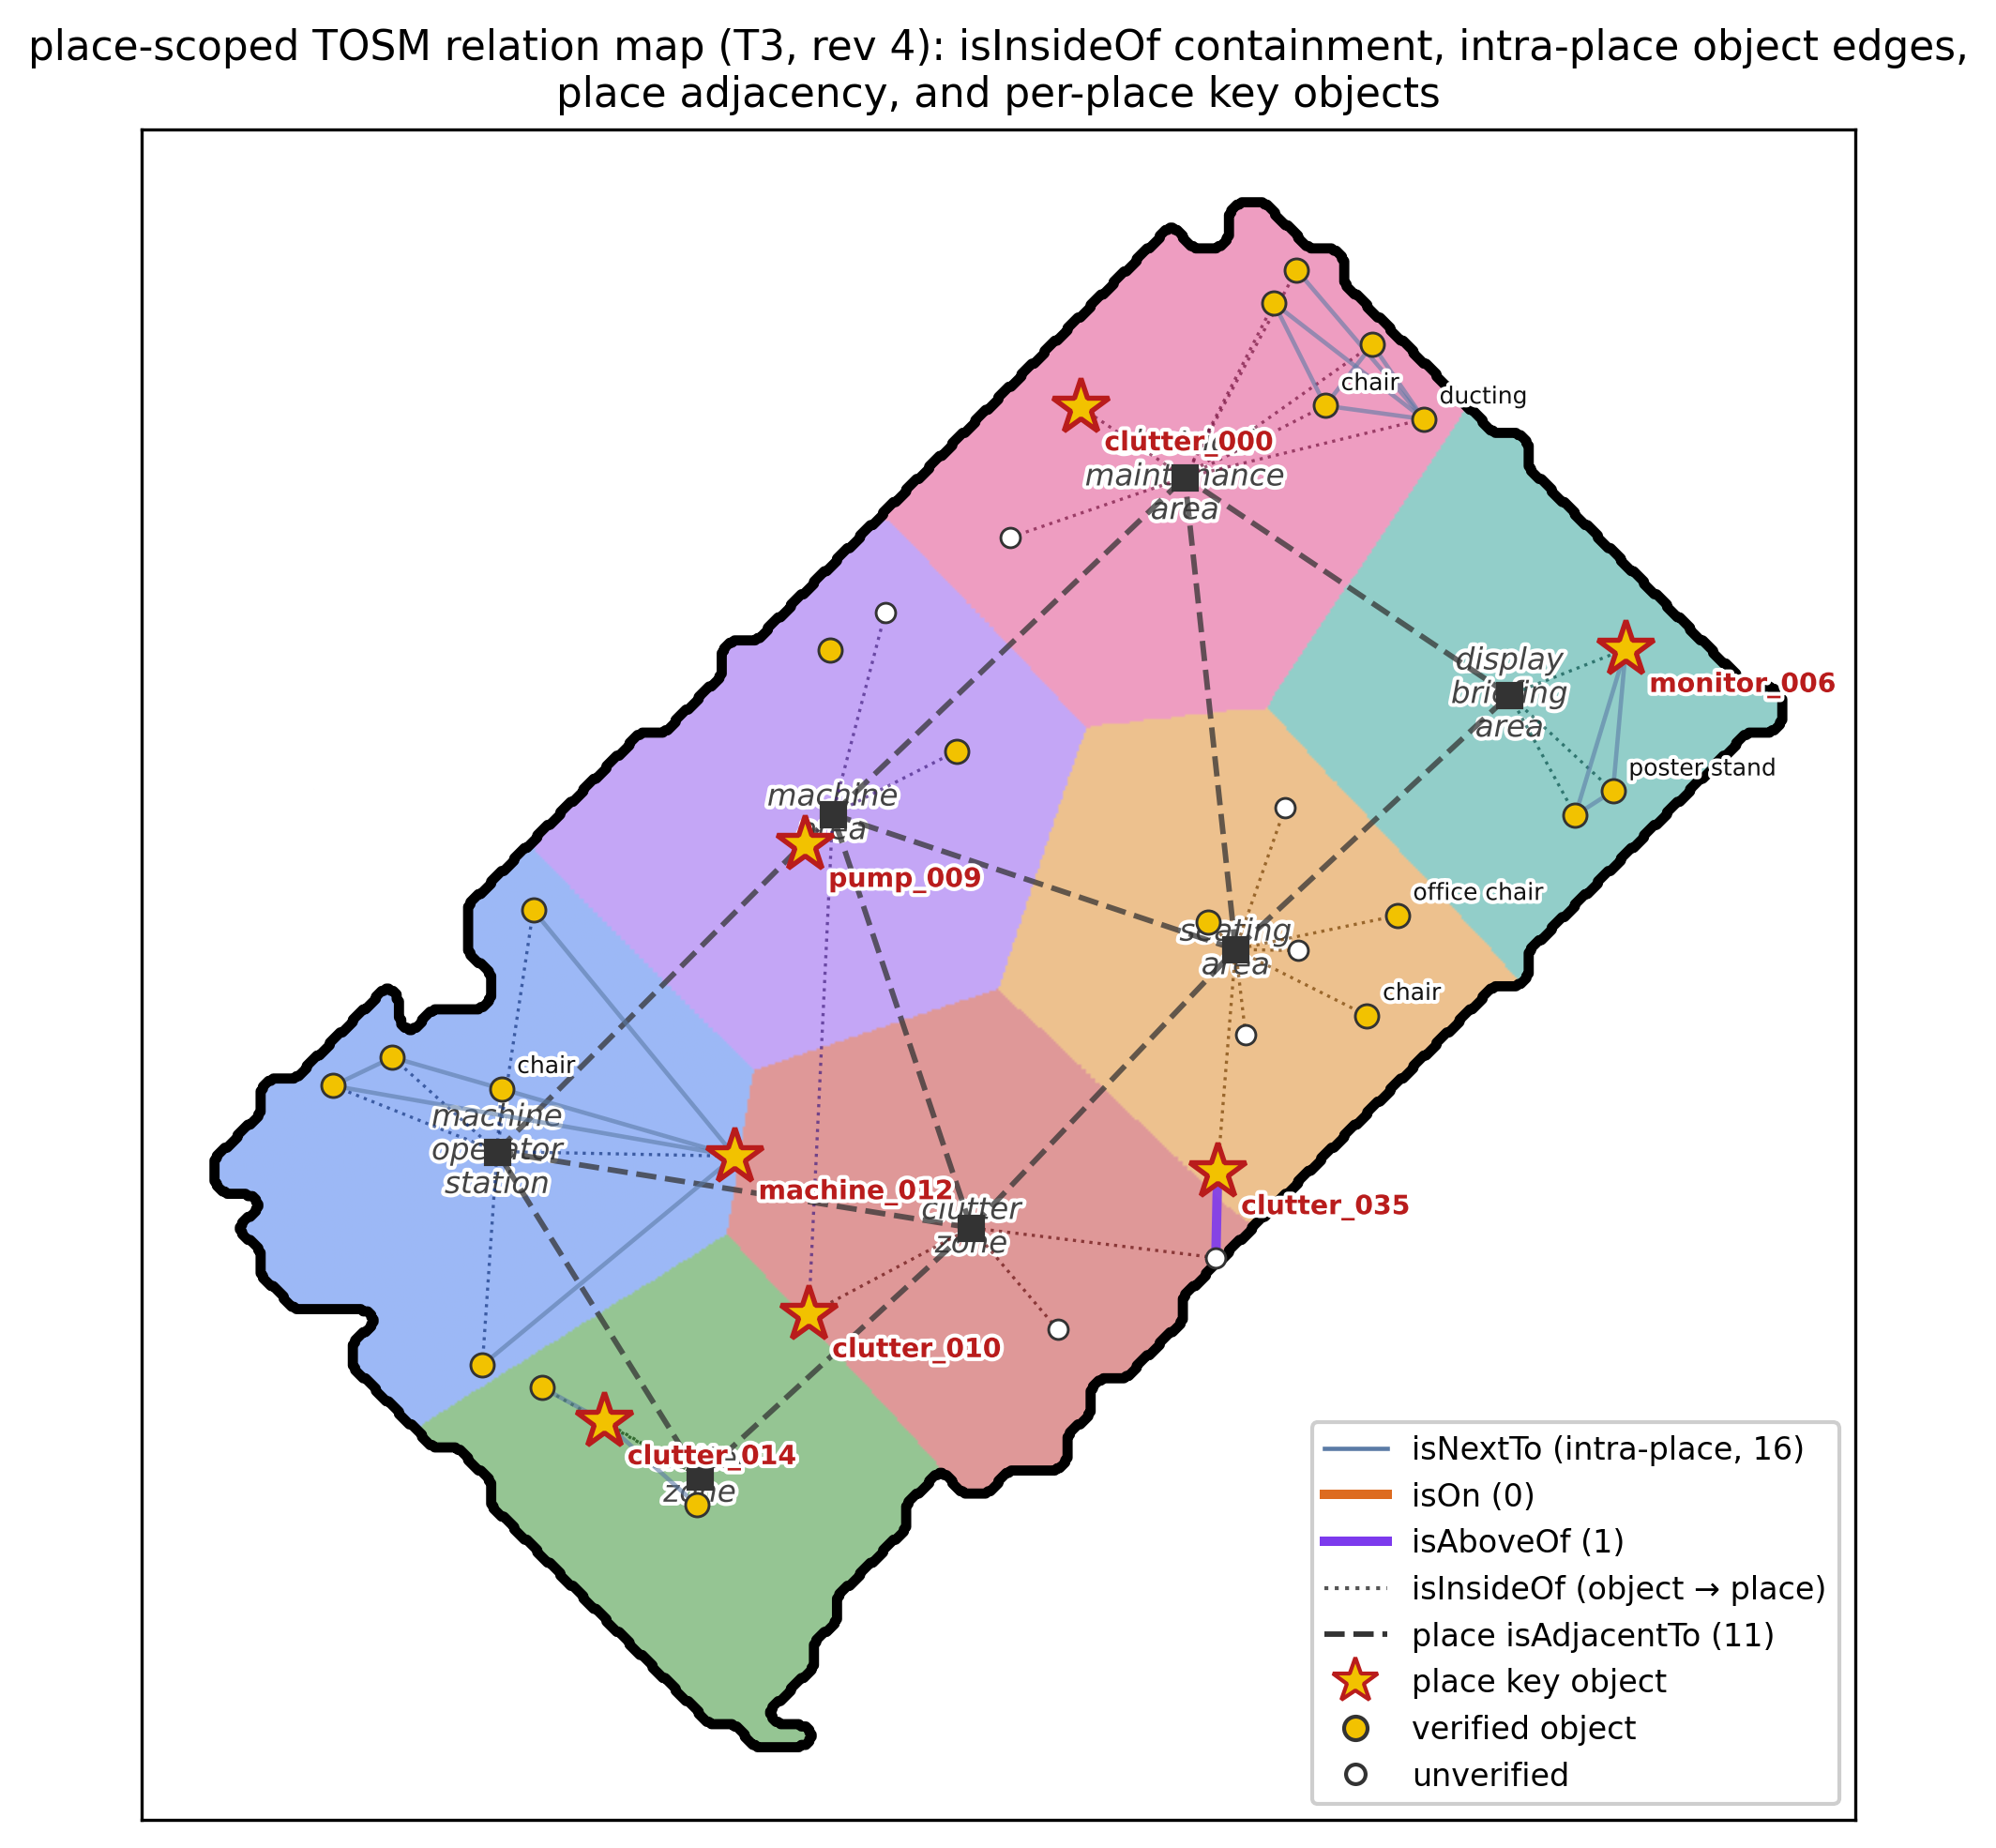
\includegraphics[width=0.85\linewidth]{figures/ele_fig12_relations_map.png}
\caption{Place-scoped TOSM relation map over the place layer of
Figure~\ref{fig:placemap}: dotted object$\rightarrow$place \texttt{isInsideOf}
containment, intra-place \texttt{isNextTo} edges, vertical
\texttt{isOn}/\texttt{isAboveOf} relations, dashed place \texttt{isAdjacentTo}
edges between region centroids, and per-place key objects (named stars).}
\label{fig:relmap}
\end{figure}

\section{Corrective Decomposition Layers and Owner Feedback}
\label{sec:corrective}

The backbone of Section~\ref{sec:backbone} is deliberately conservative, and
its characteristic failures---diffuse residual webs, wall-flush compounds
amputated by structure removal, structure noise that survives plane removal,
and real objects absorbed into \texttt{clutter}---are corrected by five layers.
The first four are automatic and run inside the frozen pipeline on every epoch;
the fifth is the human-in-the-loop channel. All were developed in response to
failures observed on the development epochs; their definitions, triggers, and
parameters were frozen before the cross-floor evaluation and require no
per-scene adjustment at execution.

\begin{enumerate}
\item \textbf{Diffuseness-gated re-split.} Trigger: a cluster whose 2D
occupancy fill (10~cm grid) is below 0.30 while its footprint exceeds
5~m$^2$---real objects fill 0.5--0.85. The cluster is re-decomposed by
occupancy-core erosion: grid cells with $\ge$8 points and $\ge$3 occupied
8-neighbors seed connected components; components with $\ge$250 points survive.
Compounds are further split at the support plane (the $z$-histogram peak
0.5--0.95~m above floor), with grounded cells spanning $>$1.3~m vertically
treated as legs or poles, and under-slab fragments re-attached at $\ge$60\%
footprint overlap. An evidence gate ($\ge$250 points, $\ge$5~m$^2$ or 12~m$^2$
for desk banks, $\ge$0.15~m height) keeps only physically plausible
sub-objects.
\item \textbf{Wall-compound gate.} Trigger: $\ge$25\% of a cluster's points
within 0.12~m of the exploration-grid wall line over a span of $\ge$2~m, with
$\ge$250 points protruding off-wall, and the cluster not diffuse. The wall
band is stripped, the support plane is detected as above, and the panel band
is cut at density valleys along the wall, yielding unit-level decomposition of
wall-mounted equipment. A final \emph{panel square-up} pass re-assigns every
compound point that falls inside a panel unit's bounding box, padded by 6~cm
horizontally and 5~cm vertically, back to that unit; it is
instance-segmentation finishing with no semantic input.
\item \textbf{Structure-condition ensemble.} Trigger: every epoch. The
geometric pass is repeated under three structure-removal conditions (none /
ceiling-only / full); clusters found under an alternative condition but absent
from the production set become new candidates, and only those are sent to
verification. Cross-condition label agreement is stored per object as a
\texttt{labelStability} attribute that prioritizes owner review;
cross-condition \emph{voting} is deliberately not used to fuse labels, because
verifier biases proved correlated across conditions.
\item \textbf{Hybrid grid-map structure filter.} Trigger: every epoch, after
clustering. Each cluster is registered against the exploration occupancy grid
of Chapter~\ref{ch:mapping}---an independent, drift-free wall prior---and
flagged by the first matching rule of a fixed cascade: outside-room ($>$50\% of
points beyond the filled room polygon), ceiling fixture (bottom $>$2.0~m above
floor), wall remnant (fraction of points within 0.15~m of the nearest grid wall
line $>$0.6 with PCA minor extent $<$0.22~m and a horizontal minor axis), or
full-height wall band ($z$-span $>$2.5~m, per-meter-segment median thickness
$<$0.3~m, along-wall length $>$2~m---the length condition spares wall-mounted
panels). Flagged clusters are removed upstream of verification.
\item \textbf{Owner feedback and gated recovery.} The management console
exposes four operations, each applied as a normal graph revision with
history: \emph{declare} (sets \texttt{verified\_owner} at confidence 1.0),
\emph{refute} (sets \texttt{refuted}, presence \texttt{absent}, and exclusion
from key-object designation), \emph{correct} (label or attribute in place, the
VLM verdict retained in provenance), and \emph{re-verify}. Recovery
re-verification re-asks the verifier with \texttt{clutter} treated as
\emph{unidentified}, in two independent passes (open vocabulary; site
vocabulary plus provisional candidates); a recovered label is adopted---as
\texttt{verified\_recovery}---only when the two passes agree under canonical
synonym matching, or a pass agrees with the cluster's own base label, and the
label is not \texttt{clutter}; a focused tie-break pass re-asks with exactly
the two disputed labels and is accepted only at confidence $\ge$0.6. A coarse
three-level height attribute (low/mid/high relative to the 2D-lidar scan plane
and the ceiling) is injected as a hard physical constraint in these passes and
stored as a queryable explicit attribute.
\end{enumerate}

The owner is not a fallback annotator but the highest-trust evidence source in
a permanently open loop: owner ground truth is itself \emph{time-variant}
(an object refuted as absent may later be declared present again when the room
changes), which is why feedback is recorded as evidence with history rather
than as immutable truth, and why one correction propagates through the object,
relation, place, scene, and mission layers at once from a single write.

\section{Query Interface with Structural Gating}
\label{sec:query}

The graph is queried through an LLM that receives a
serialized view of the relevant nodes. The naive design---instructing the
model not to assert unverified labels---fails in practice: in the benchmark of
Section~\ref{sec:exp-ablation} the instructed model still asserted trap labels
in 3 of 4 cases. The framework therefore \emph{gates by construction, not
exhortation}: in the query-time view, every unverified node's type is demoted
to \texttt{unknown}, and the failed candidate label is moved to a separate
\texttt{failedCandidateType} field whose semantics (``a classifier guess that
did not survive verification'') are stated in the schema, not in behavioral
instructions (Figure~\ref{fig:cards}). With the gate in the data rather than
the prompt, the model cannot assert an unverified label without visibly
contradicting its input. Traps whose label was wrongly \emph{verified} lie
beyond any status-based gate---a bound quantified in
Section~\ref{sec:exp-query}. In interaction, the gate makes confidence part of
the answer rather than metadata: asked whether there is a keyboard in the room,
the system asserts a verified keyboard with its location, while an unverified
one yields ``an object at $(x,y)$ was proposed as a keyboard by the classifier
but did not pass verification''---an answer a robot can act on conservatively.

\begin{figure}[!htb]
\centering
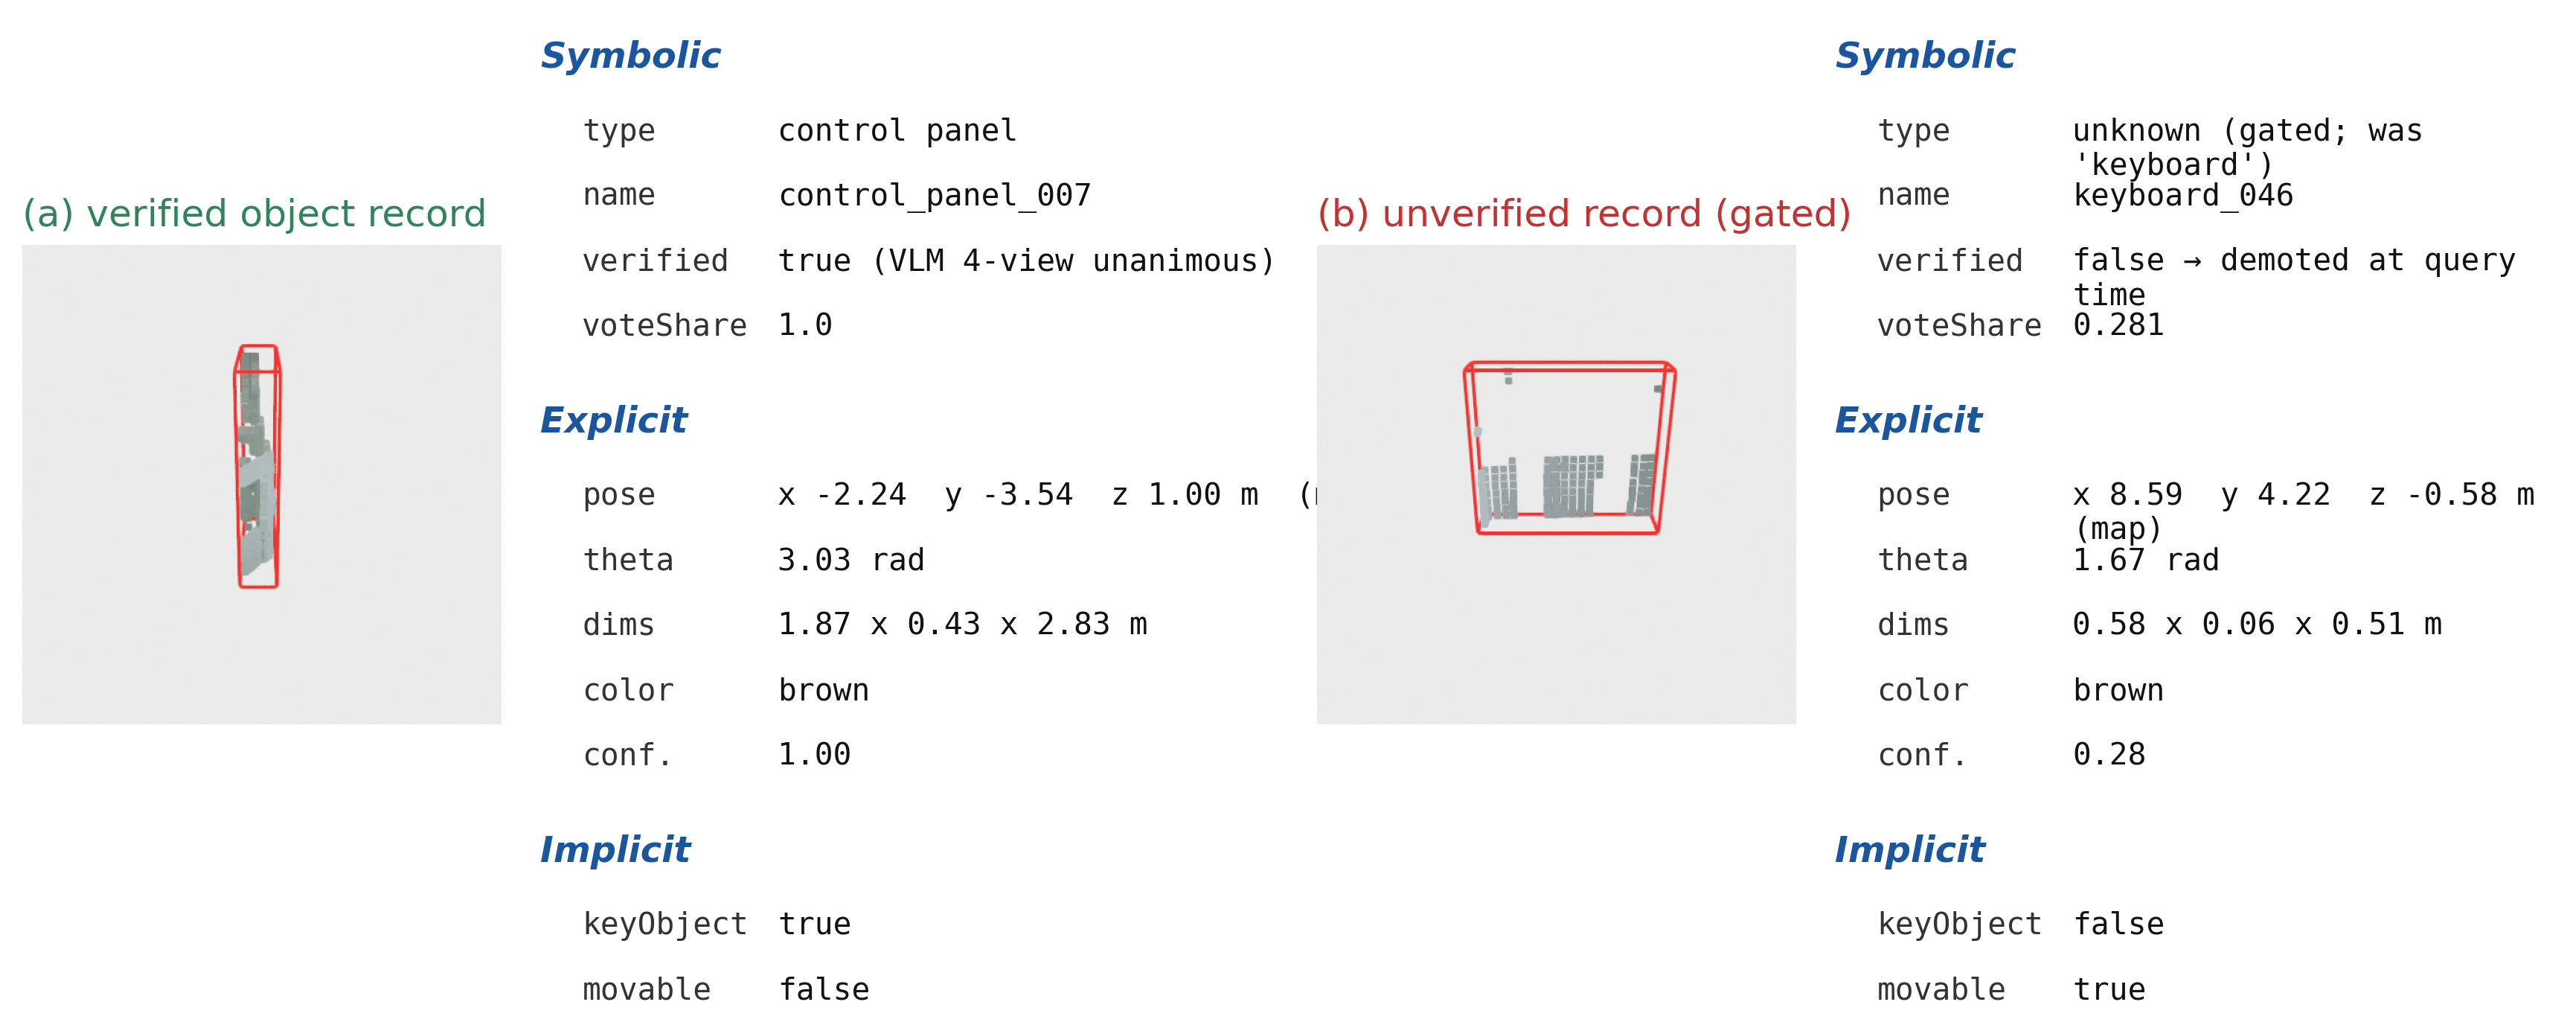
\includegraphics[width=0.95\linewidth]{figures/ele_fig4_record_cards.png}
\caption{TOSM semantic-object records (symbolic / explicit / implicit layers).
(a)~A verified record asserts its type. (b)~An unverified record is
structurally gated at query time: the type is demoted to \texttt{unknown} and
the failed classifier guess is quarantined in \texttt{failedCandidateType}.}
\label{fig:cards}
\end{figure}

\section{Object-Grounded Place Layer}
\label{sec:place}

Robot tasking refers to places (``the docking area'') as often as to objects.
Following the TOSM place schema of DK-SMF~\cite{joo2025dksmf}---boundary
polygon, containment, and purpose---the framework adds a place layer grounded
in the verified object layer. Place regions are obtained automatically from
the robot-facing occupancy grid map (0.05~m; the exploration SLAM map of
Chapter~\ref{ch:mapping} on deployment, or a grid synthesized from the scan's
floor points where no exploration run exists): the room interior delimited by
the mapped outer boundary is partitioned by SLIC superpixel
segmentation~\cite{achanta2012slic} with the number of superpixels as the
governing parameter (seven requested here), fragments below an area threshold
(1.5~m$^2$) are discarded, and each region's centroid is the moment-based
center of its cells (cf.\ grid-map room
segmentation~\cite{bormann2016room,luperto2022robust}). Each object's
\texttt{isInsideOf} resolves to the region containing its anchor cell. Each
place is then summarized by its \emph{ring code}: the sequence of member
objects sorted by bearing around the place centroid---restricted to
verified-tier objects, so the confidence gate propagates into place
semantics---and a single LLM call names the place from its ring code. Because
the segmentation depends only on the map, region identity is stable across
scan epochs, and the same regions re-derive names that track the room's actual
use without manual re-annotation (Section~\ref{sec:exp-update}).
Figure~\ref{fig:placemap} shows the resulting place layer. The robot layer of
TOSM is instantiated from the platform description in
Chapter~\ref{ch:validation}.

\begin{figure}[!htb]
\centering
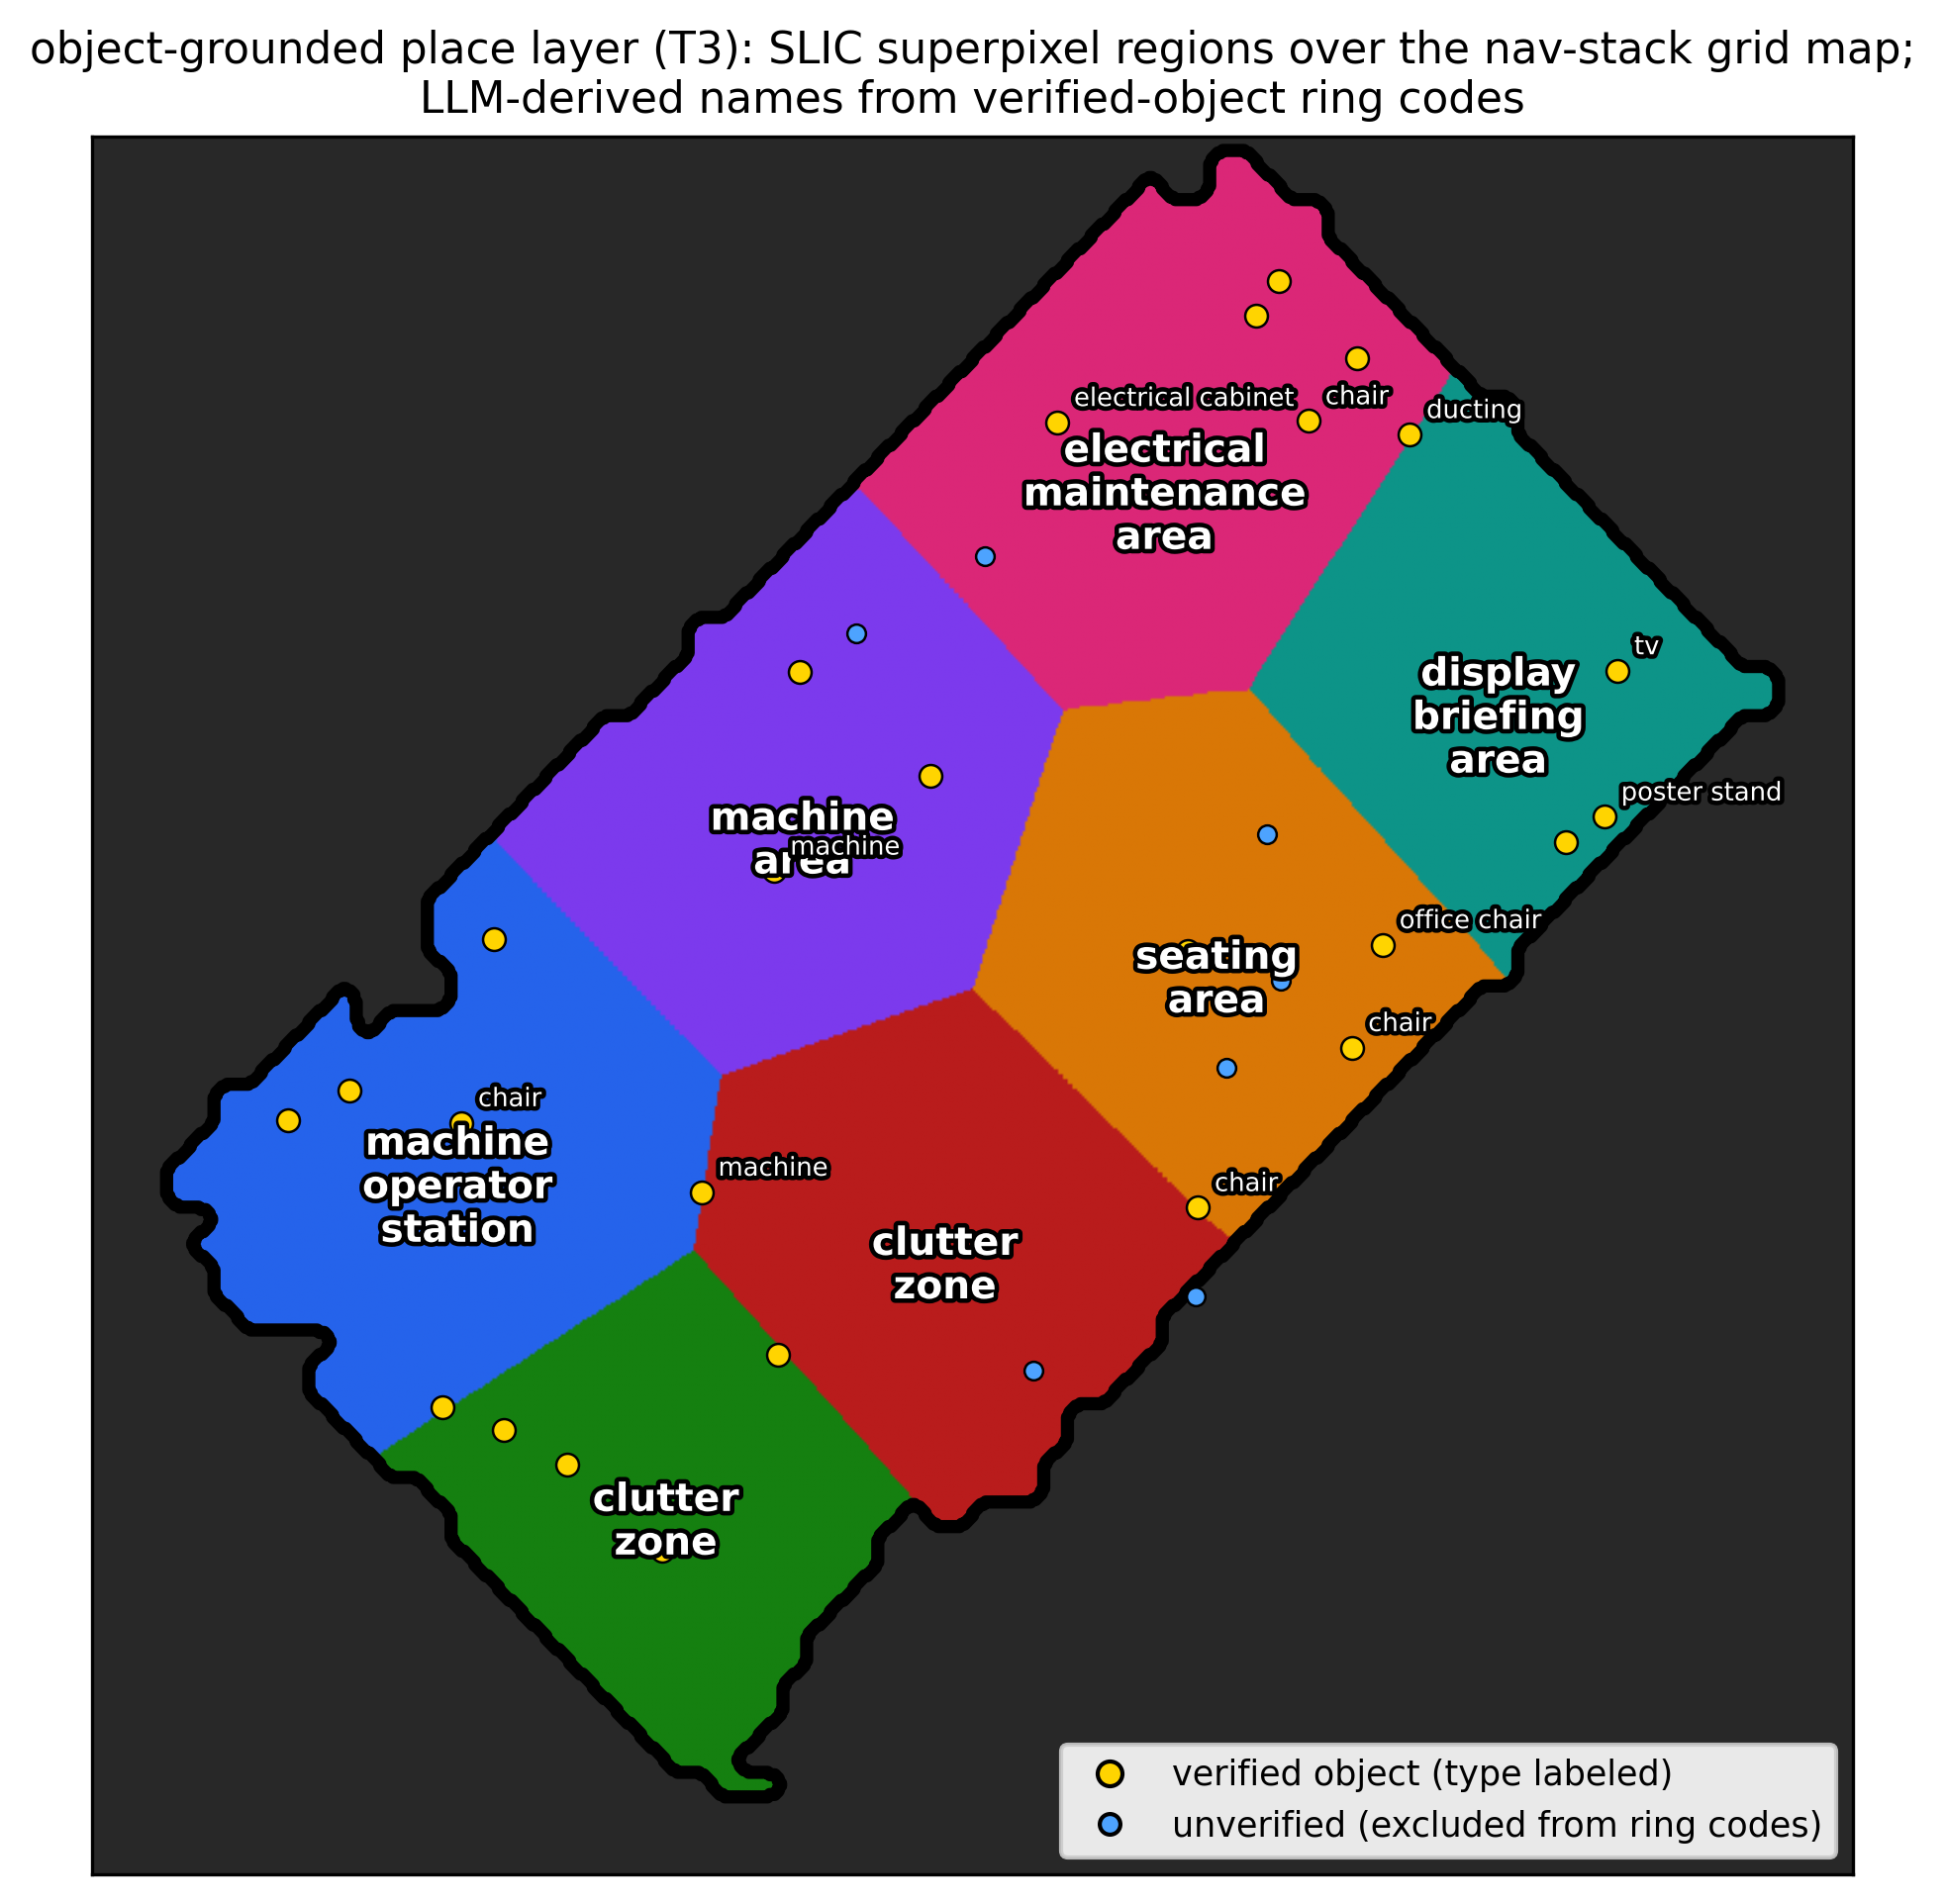
\includegraphics[width=0.85\linewidth]{figures/ele_fig11_place_map.png}
\caption{Object-grounded place layer. SLIC superpixel regions tile the room
interior delimited by the navigation grid map's outer boundary and carry
LLM-derived names computed from verified-object ring codes; unverified objects
(blue markers) do not contribute, so the confidence gate propagates into place
semantics.}
\label{fig:placemap}
\end{figure}

\section{Multilayer Robot-Consumable Representation}
\label{sec:layers}

From the same 3D semantic model, the framework derives the layers that
spatial operations at different heights require, so that the representation
remains compatible with conventional 2D-laser-based navigation stacks while
exposing the vertical structure that a mobile manipulator or a lifting
platform needs (Figure~\ref{fig:layers}). Three vertical bands are defined
relative to the estimated floor plane $z_0$.

\begin{itemize}[leftmargin=2.2em,itemsep=2pt]
  \item \textbf{Driving layer} ($z_0+0.10$ to $z_0+1.80$~m). Points in the
        band relevant to a mobile base are rasterized into a 2D occupancy grid
        at 0.05~m resolution and exported in the ROS map format, so that the
        simulated and real navigation stacks share one map
        (Section~\ref{sec:scan2sim}); the exploration SLAM map of
        Chapter~\ref{ch:mapping} is the equivalent product on a deployment
        where the robot itself mapped the space. The place layer of
        Section~\ref{sec:place} is defined on this grid.
  \item \textbf{Manipulation work layer} (reach band of the platform,
        $z_0+0.4$ to $z_0+1.6$~m for the AMMR). The explicit models of every
        verified object whose extent intersects the band provide the
        footprints, poses, top heights, and movability from which a mission
        mediator computes approach poses and clearance checks against the
        robot's own footprint (Section~\ref{sec:missions}) and from which a
        manipulation planner screens coarse feasibility; no separate
        rasterization is needed because the object records already carry
        metric 3D extents.
  \item \textbf{Overhead layer} (above the driving band, up to the ceiling).
        Ceiling-mounted structure---fixtures, ducts, cable trays, beams, and
        installation targets---is recognized by the overhead recognition
        module of Section~\ref{sec:overhead} from the pre-removal ceiling
        reference cloud that the backbone retains, verified under the same
        protocol, and merged into the graph with \texttt{heightLevel = high},
        so that a pointing or installation task can be resolved to a metric
        overhead target in the map frame.
\end{itemize}

Each band is a view over one graph rather than a separate model: an object
record carries its full 3D extent, and band membership is a query. The
simulation layer of Chapter~\ref{ch:validation} injects the same records
into a physics-enabled stage. The driving band and the place layer are
exercised end to end on the physical robot in Section~\ref{sec:exp-missions};
the overhead band is evaluated in Section~\ref{sec:exp-overhead}.

\begin{figure}[!htb]
  \centering
  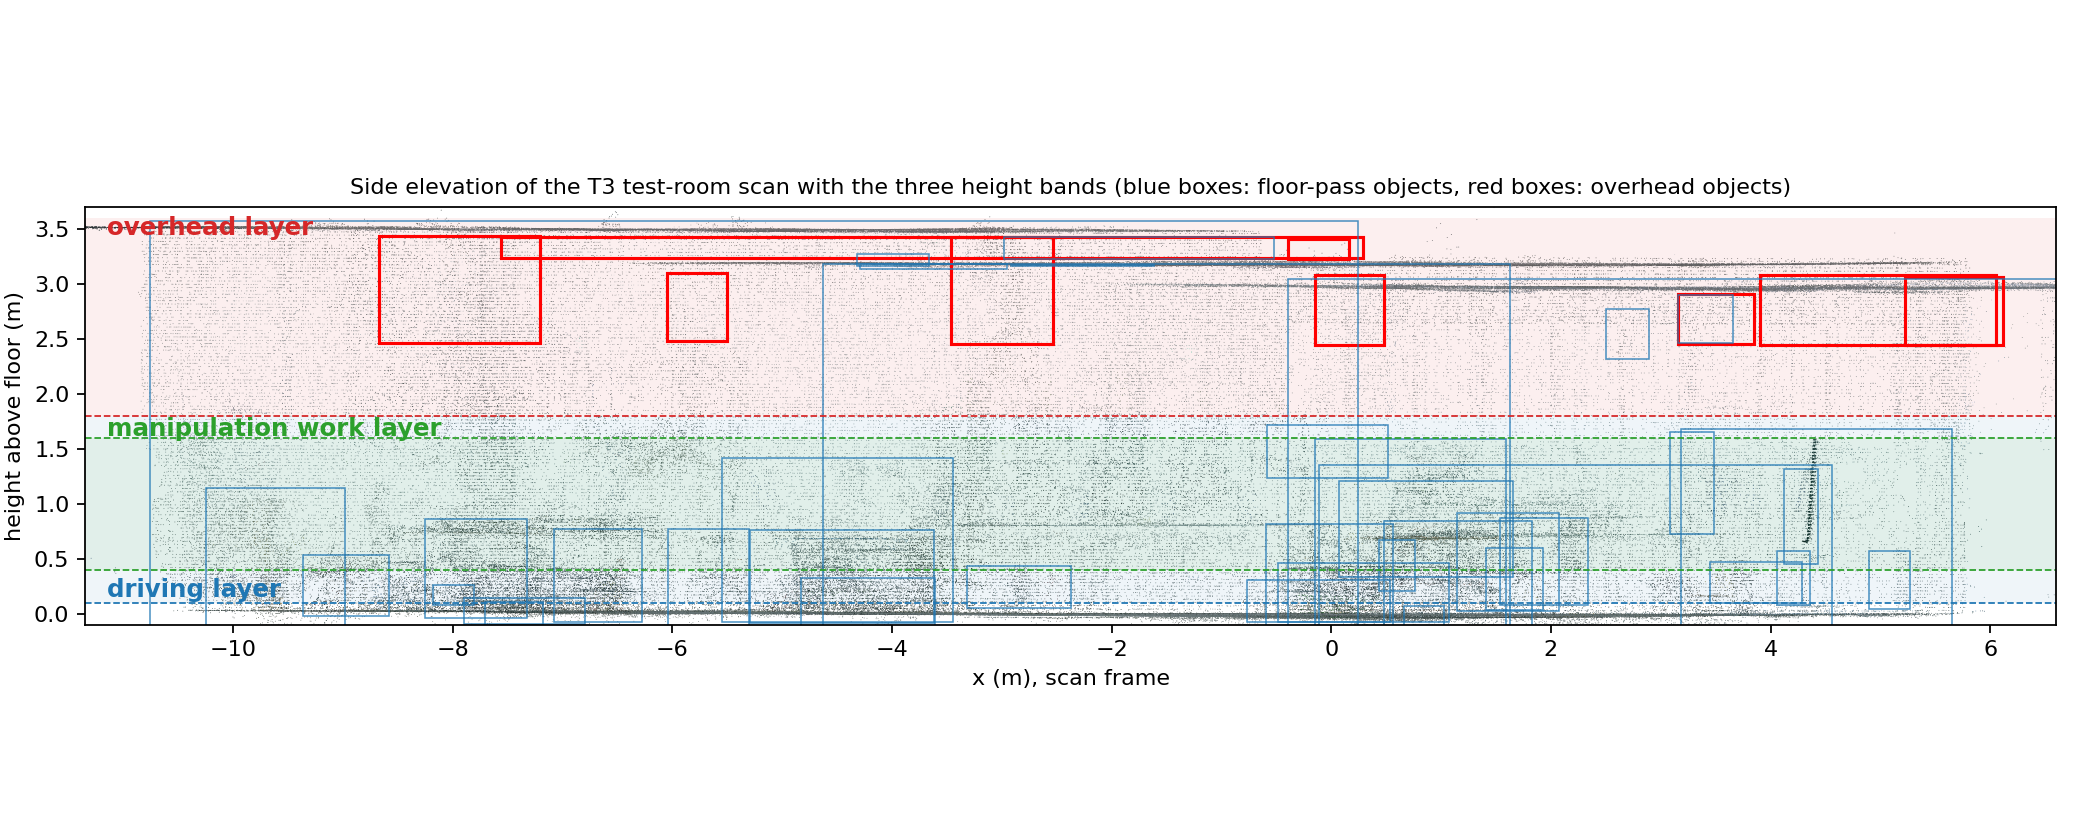
\includegraphics[width=0.95\textwidth]{figures/fig4_layers.png}
  \caption{Multilayer robot-consumable representation. The driving layer
  (occupancy grid and place layer), the manipulation work layer (verified
  object extents at reach height), and the overhead layer (ceiling-mounted
  structure from the overhead recognition module) are three height-band views
  over the one knowledge graph; a mobile manipulator consumes all three.}
  \label{fig:layers}
\end{figure}

\section{Overhead Structure Recognition}
\label{sec:overhead}

A strength of survey-grade TLS is that it captures the ceiling as faithfully
as the floor, yet the backbone of Section~\ref{sec:backbone} removes the
ceiling planes and discards everything attached to them in order to isolate
floor-standing objects. The overhead recognition module recovers that
content as a complementary pass that is appended to the frozen pipeline and
merged with the floor-level graph, without altering the object-level
algorithm validated in Sections~\ref{sec:exp-seg}--\ref{sec:exp-endtoend}.

The module operates on the pre-removal \emph{ceiling reference} cloud that
the backbone retains (Section~\ref{subsec:preprocess}), colored from the raw
scan by the same deterministic downsampling, and proceeds in six steps with
the parameters fixed once and applied unchanged to every scene.
\begin{enumerate}[leftmargin=2.2em,itemsep=2pt]
  \item \emph{Overhead band.} The floor height is estimated as in the
        remnant filter, and only points more than 1.80~m above it---the top
        of the driving band---enter the pass.
  \item \emph{Ceiling levels.} Near-horizontal planes ($|n_z|\ge0.85$) are
        extracted from the band by the same seeded RANSAC as the structure
        removal, up to four levels, so that multi-level ceilings are
        represented explicitly; points within $\pm0.06$~m of a level are
        ceiling and are excluded, as is content above the highest level
        (seen through openings).
  \item \emph{Walls.} Near-vertical planes ($|n_z|\le0.2$) are extracted from
        the remaining band points, up to eight; points within 0.12~m of a
        wall plane are wall.
  \item \emph{Floor-object exclusion.} Points that fall inside the padded
        (0.10~m) footprint of a floor-pass object and below that object's top
        are the upper part of an object the floor pass already owns and are
        excluded; merged clusters wider than 3~m are ignored for this test so
        that a mega-cluster's footprint cannot swallow the ceiling.
  \item \emph{Decomposition and explicit model.} The remaining candidates
        are clustered by the floor pass's DBSCAN ($\varepsilon=0.30$~m, 80
        points minimum) with the same conservative giant-split, and each
        cluster receives the same explicit model (extent, centroid, yaw,
        color) plus three overhead attributes: the clearance below it (bottom
        above floor), the gap to the nearest ceiling level, and its
        attachment---\emph{ceiling-hung} if its top is within 0.15~m of a
        ceiling level, \emph{wall-mounted} if at least 25\% of its points lie
        within 0.22~m of a wall plane, and \emph{suspended} otherwise. The
        height level is \texttt{high} by construction. Candidates are
        room-scoped with the same mask as the floor pass, with a 0.5~m
        tolerance because wall-hung fixtures sit at the free-space boundary.
  \item \emph{Verification and merge.} A provisional label is attached by
        the same open-vocabulary classifier over an overhead vocabulary
        (light fixture, fluorescent lamp, air conditioner, ventilation duct,
        cable tray, beam, pipe, sprinkler head, projector, speaker, sign,
        surveillance camera, smoke detector, ceiling panel, curtain rail),
        the four base views and the eight escalation views are rendered from
        $30^\circ$ \emph{below} the object instead of $25^\circ$ above, and
        the late-fusion verifier of Section~\ref{sec:verification} runs
        unchanged except that the overhead vocabulary is passed as the
        candidate list and the \texttt{high} height level as a hard prior.
        Verified overhead objects enter the graph through the identity
        policy and confidence-gated upsert of
        Sections~\ref{sec:matching}--\ref{sec:upsert}, so that they are
        tracked across epochs like any other node; their spatial relations
        are limited to \texttt{isAboveOf} the floor-level object or place
        beneath them, which is what an installation or pointing task
        consumes.
\end{enumerate}
The structure-remnant and hybrid grid-map filters remain in force for the
floor pass and are not applied to the overhead pass, whose whole purpose is
the content those filters discard; conversely, nothing the overhead pass
finds can alter a floor-pass node, so the evaluation of
Sections~\ref{sec:exp-seg}--\ref{sec:exp-endtoend} is unaffected by enabling
it. Section~\ref{sec:exp-overhead} evaluates the pass on the two industrial
epochs and the cafeteria scene.
   % 3D Point Cloud Semantic Modeling
%%=============================================================================
%% chapters/chapter5.tex — Digital-Twin-Based Validation (final-defense version)
%%=============================================================================
\chapter{Digital-Twin-Based Validation with Spatial-Operation Robots}
\label{ch:validation}
This chapter presents the third part of the framework: the architecture
through which the semantic database produced by Chapters~\ref{ch:mapping}
and~\ref{ch:semantic} is connected to a digital twin, a management console, and
a physical spatial-operation robot, so that the integrated framework can be
evaluated as a whole.\footnote{The content of this chapter is based on the author's RAAICON~2026 paper~\cite{raaicon2026} and on the application section of the TLS-SMF manuscript submitted to \emph{Electronics}~\cite{kim2026electronics}.} Section~\ref{sec:dt-arch} states the architecture and
its single-store principle. Section~\ref{sec:scan2sim} describes the automated
scan-to-simulation pipeline that turns the registered scan into a
physics-enabled NVIDIA Isaac Sim stage, Section~\ref{sec:twin-bridge} the live
bidirectional bridge and its frame calibration, Section~\ref{sec:semantic-twin}
the injection of the semantic layer into the twin, Section~\ref{sec:missions}
the semantic mission stack, and Section~\ref{sec:real-robot} the integration
with the physical robot.

\section{Validation Architecture and Single-Store Principle}
\label{sec:dt-arch}

The crux of the validation is to confirm that a single environmental
representation simultaneously satisfies different modes of consumption. The
knowledge graph of Chapter~\ref{ch:semantic} is the \emph{single semantic
store}: the management console (a browser interface that issues mission
commands, shows the live graph and robot state, and gives the owner one-click
refute/re-type/attribute edits), the semantic mission mediator, the Isaac Sim
twin, and---through the same mediator---the physical robot all read the same
revisioned file, so a correction propagates to every consumer from a single
write (Figure~\ref{fig:dt-arch}). Consistent with the laboratory's
RaaS-oriented control server~\cite{kwon2025}, the digital twin acts as the
supply layer from which a semantic task manager draws the environmental
knowledge required for cost-aware task allocation; where the task manager
decomposes natural-language commands and allocates them to heterogeneous
robots, the present framework supplies the underlying environmental knowledge
that such allocation depends upon. The validation of this chapter therefore
aims to demonstrate that the framework's output is not merely a visualizable
model but a representation that is consumable for actual robot mission
execution.

\begin{figure}[!htb]
  \centering
  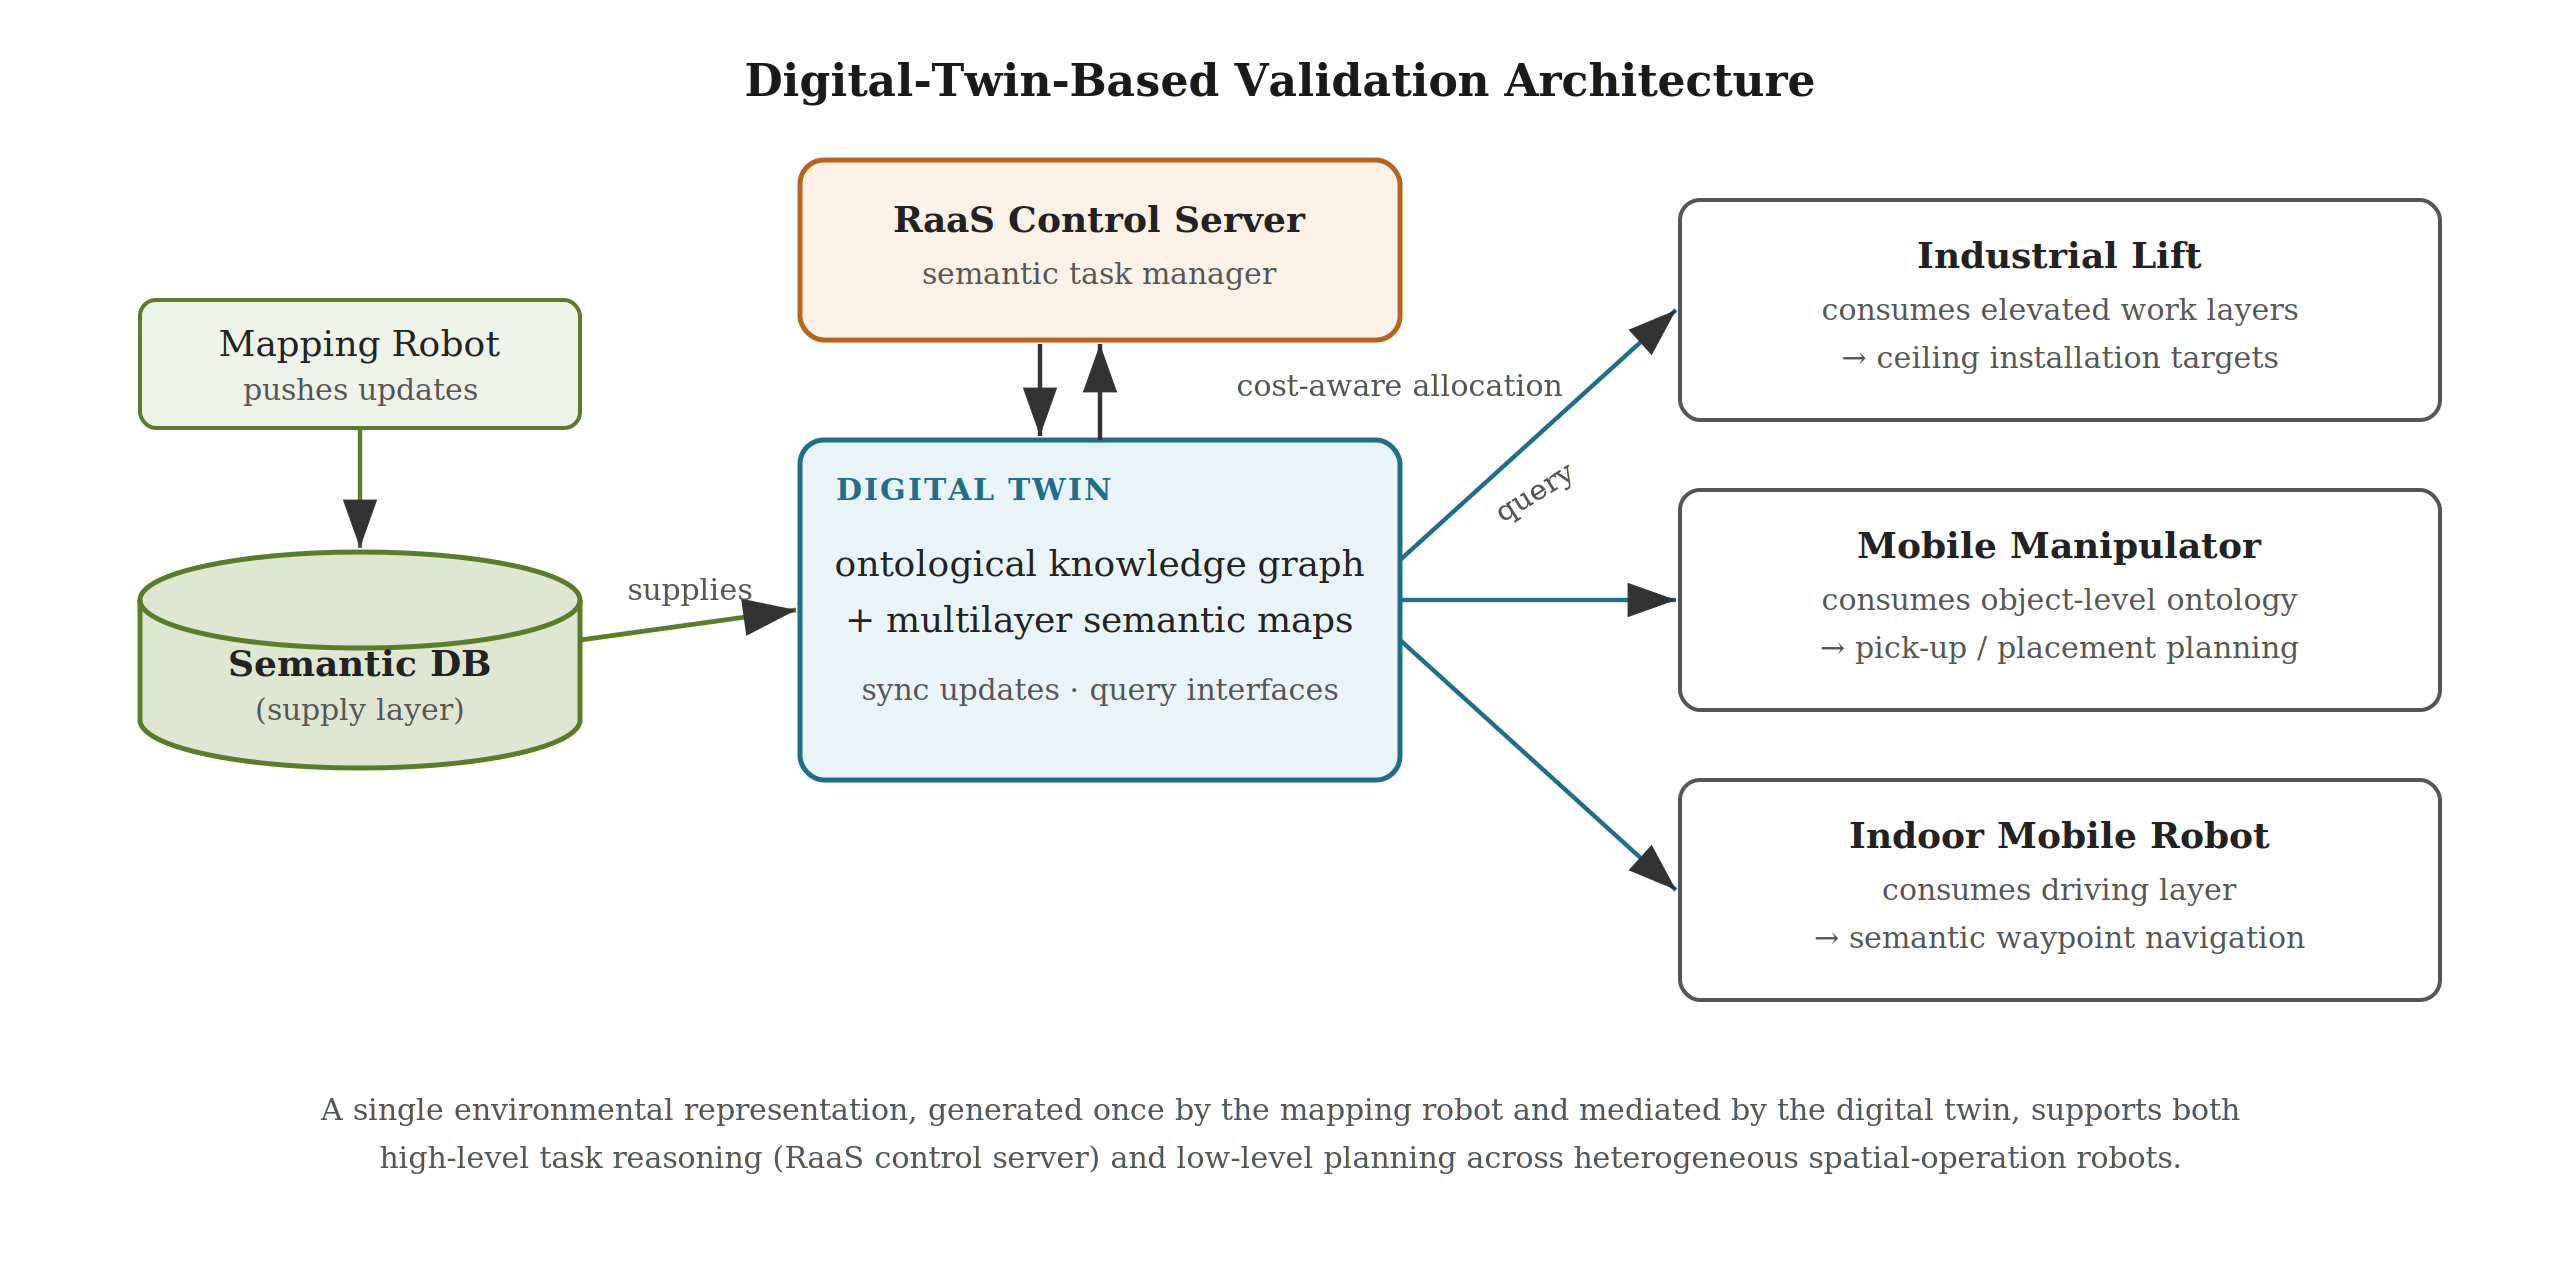
\includegraphics[width=0.95\textwidth]{figures/fig5_1.png}
  \caption{Digital-twin-based validation architecture. The semantic database
  supplies a digital twin connected to a RaaS-oriented control server;
  downstream robots consume the shared representation through query
  interfaces. In this dissertation the chain is validated with a swerve-drive
  mobile manipulator (AMMR), a single platform that spans the driving,
  manipulation, and overhead bands of the same store.}
  \label{fig:dt-arch}
\end{figure}

The validation platform is the AMMR, a swerve-drive autonomous mobile
manipulator robot deployed in the industrial test room in which all
experiments are conducted. A mobile manipulator is a natural single-platform
consumer of the multilayer representation of Section~\ref{sec:layers}: its
base navigates on the driving layer, its arm operates in the manipulation work
layer, and its end effector can be directed at targets in the overhead layer.
The experiments of Chapter~\ref{ch:experiments} exercise the driving band end
to end on hardware (console-issued semantic missions) and the manipulation and
overhead bands at the representation level (verified object poses and
footprints at reach height, and ceiling-mounted structure recognized from the
same scan), which is the contract a manipulation or installation planner
consumes.

\section{Scan-to-Simulation Pipeline}
\label{sec:scan2sim}

Constructing a simulation environment that faithfully reproduces a real
indoor workspace is a major bottleneck when deploying digital twins: scenes are
typically modeled by hand, which is slow, subjective, and quickly outdated. A
raw point cloud is not a simulation environment either: it has no collision
representation, no gravity-aligned reference frame, and no interface to a
robot simulator. The pipeline of Figure~\ref{fig:raa-pipeline} converts the
merged E57 export automatically into a physics-ready Isaac Sim USD stage. It
deliberately keeps two decoupled layers---a coarse collision layer derived
from the occupancy grid and a dense point layer for appearance---which keeps
conversion fast, robust to scan noise, and directly navigable by a mobile base,
rather than reconstructing a watertight mesh.

\begin{figure}[!htb]
\centering
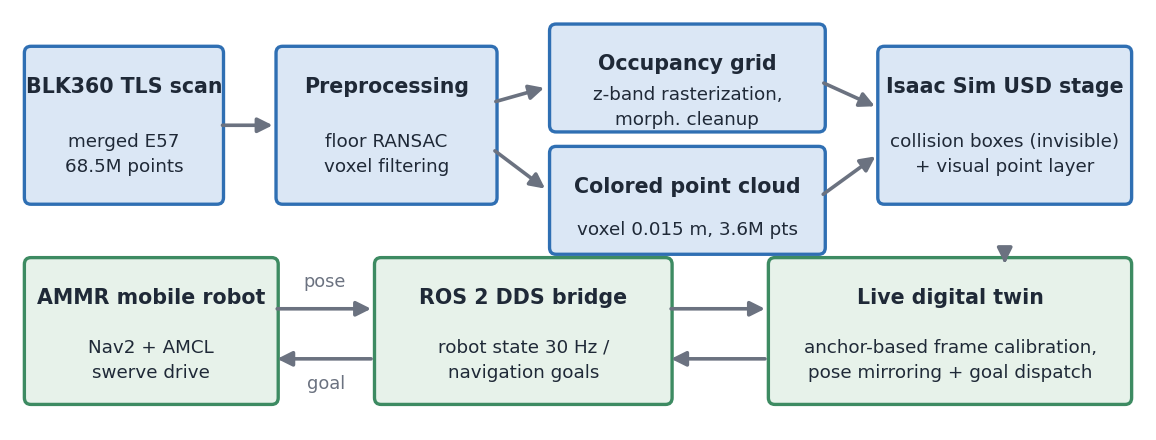
\includegraphics[width=0.9\linewidth]{figures/raa_fig_pipeline.png}
\caption{Scan-to-simulation system overview. Offline (top): the merged BLK360
E57 export is converted into an occupancy grid, a collidable wall layer, and a
dense colored point layer composing the Isaac Sim stage. Online (bottom): a
ROS~2 DDS bridge mirrors the robot pose at 30~Hz and returns navigation goals
selected in the simulator.}
\label{fig:raa-pipeline}
\end{figure}

\subsection{Preprocessing and Floor-Plane Estimation}
\label{subsec:s2s-preproc}

The pipeline first estimates the dominant floor plane with RANSAC on a
voxel-thinned subset of the merged cloud, yielding the gravity-aligned
reference frame and the floor height $z_0$; all subsequent layers are expressed
relative to this frame, so no manual leveling or origin selection is required.
In the test room, the registered stations were exported as a single E57 file
of 68.5~M points (1.3~GB); scan placement followed the visibility-coverage plan
of Chapter~\ref{ch:mapping}.

\subsection{Occupancy Grid and Collision Layer}
\label{subsec:s2s-occ}

Points within the height band $[z_0{+}0.10,\ z_0{+}1.80]$~m---the band relevant
for a mobile base---are rasterized into a 2D occupancy grid at 0.05~m
resolution. Morphological cleanup removes speckle from reflections and small
blobs below 0.02~m$^2$. The occupied cells are then greedily merged into
axis-aligned boxes and emitted as USD cubes of 2.5~m height with physics
collision enabled. Crucially, the collision boxes are marked \emph{invisible}:
they provide physics without occluding the visual point layer. The same
occupancy grid is exported in the ROS map format so that the simulated and real
navigation stacks can share one map; it is the driving layer of
Section~\ref{sec:layers}.

\subsection{Visual Point-Cloud Layer}
\label{subsec:s2s-visual}

For appearance, the full-resolution colored cloud is voxel-downsampled to
0.015~m (3.6~M points, ceiling included) and embedded as USD point primitives
with per-point color and a rendered point width of 0.013~m, chosen at
approximately 0.85 times the voxel size so that points visually fuse into
surfaces at navigation-relevant viewing distances. The two-layer design keeps
the stage lightweight: collision queries run against about 1{,}430 boxes rather
than millions of points, while the operator sees the photographic appearance of
the real room.

\subsection{Robot Model and Mobile-Base Control}
\label{subsec:s2s-robot}

The AMMR is a swerve-drive mobile manipulator with two independently steered
wheel modules mounted diagonally at $\mathbf{p}_{1,2}=(\pm0.364,\ \mp0.137)$~m
and four passive casters; its URDF (12 links, 11 joints) was authored from the
manufacturer's 2D drawings. For simulation-only operation the base is
velocity-controlled through the standard inverse kinematics: for a commanded
body twist $(v_x, v_y, \omega)$ each module $i$ tracks
\begin{equation}
\mathbf{v}_i = \begin{bmatrix} v_x - \omega\, p_{i,y} \\
v_y + \omega\, p_{i,x} \end{bmatrix},\quad
\delta_i = \operatorname{atan2}(v_{i,y}, v_{i,x}),\quad
\dot\varphi_i = \frac{\lVert \mathbf{v}_i \rVert}{r},
\label{eq:swerve}
\end{equation}
with wheel radius $r=0.075$~m. Steering angles are wrapped to
$[-90^\circ, 90^\circ]$ with wheel-speed reversal; a hysteresis of 0.12~rad on
the reversal decision and a cosine speed gate suppress the flip-flopping that
otherwise occurs when a module operates exactly at the wrap boundary, for
example during pure rotation. The TOSM robot layer (footprint, drive type,
sensor mounts, velocity limits) is instantiated from the same URDF and
navigation configuration and ingested alongside objects and places, completing
the three-element TOSM model; the same layer drives the Gazebo proxy of
Section~\ref{sec:missions}.

\section{Live Twin Bridge and Frame Calibration}
\label{sec:twin-bridge}

During live operation the simulated robot is switched to kinematic mode and
mirrors the real pose. The robot publishes its localized pose (AMCL
localization~\cite{dellaert1999} on its own navigation map) as a 30~Hz
odometry stream; the simulator subscribes over a DDS bridge (Cyclone
DDS~\cite{cyclonedds}, a dedicated ROS~2 domain, unicast peer configuration
over Wi-Fi) and applies the pose each physics step. In the reverse direction,
dragging a goal marker in the simulator publishes a goal pose that an on-robot
relay forwards to the robot's Nav2 stack~\cite{macenski2020marathon}, closing
the loop: the physical robot navigates to targets picked in the twin.

The robot's SLAM map frame and the scan frame differ by an unknown planar rigid
transform. It is calibrated with a single anchor: the robot is parked at a
physically identifiable spot whose scan-frame pose $(\mathbf{a}, \theta_a)$ is
known---in the test room the robot itself was captured in the scan, so its
scanned footprint provides the anchor; a taped start spot of known scan
coordinates serves the same purpose in later sessions. On receipt of the first
live pose $(\mathbf{r}, \theta_r)$ the offset follows in closed form,
\begin{equation}
\theta_{\mathrm{off}} = \theta_a - \theta_r, \qquad
\mathbf{t}_{\mathrm{off}} = \mathbf{a} - R(\theta_{\mathrm{off}})\,\mathbf{r},
\label{eq:anchor}
\end{equation}
and is reused for all subsequent poses and goals. The one-shot calibration
inherits the localization error of the single pose sample it is computed from:
any AMCL error at anchor time becomes a permanent bias of the session, and
across on-site sessions the recovered offsets differed by up to 0.60~m and
$9.1^\circ$, reflecting run-to-run differences in AMCL initialization rather
than scene error. The operating procedure therefore verifies the overlay
visually after anchoring (a short teleoperated advance must move the twin in
the same direction as the robot) and re-anchors if the twin is misaligned.
Averaging over multiple anchor poses, or refining the offset by matching the
live 2D-lidar scan against the TLS cloud, would remove the single-sample
dependence.

\section{Semantic Twin Injection}
\label{sec:semantic-twin}

Because every node of the knowledge graph carries an explicit model in the
scan frame, the graph can be injected directly into the simulation stage. The
digital twin of Section~\ref{sec:scan2sim} is extended with the semantic
layer: the stage is re-derived from the graph whenever the graph changes, each
verified object spawning a labeled proxy (extent box or segmented cloud) with
its verification status, provenance, height level, and label stability exposed
in a scene inspector, while unverified objects spawn as neutral gray
placeholders---the gate is visible in the twin. A file watcher converts the
current graph revision to a USD layer and the running stage reloads it, so an
owner edit in the console propagates to the robot's next goal, the console,
and the twin from one write. The discipline is self-auditing: deriving the
stage from the graph immediately visualized eighteen stale earlier-epoch nodes
as orphan boxes that per-view export paths had silently hidden, prompting the
cleanup revision reported in Section~\ref{sec:exp-update}.

\section{Semantic Mission Stack}
\label{sec:missions}

The loop from scan-derived knowledge to autonomous behavior is closed by a
mission stack with three components. A \emph{semantic mediator} resolves
high-level mission commands---\texttt{goto\_place}, \texttt{goto\_object},
\texttt{patrol}, \texttt{return\_home}---against the knowledge graph: places
resolve to free-space points at region centroids, objects to approach poses
computed from the target's footprint and the robot's circumscribed radius (the
kinematics-aware resolution style of TOSMNav~\cite{joo2022fsom}), with the
verification gate deciding eligibility; a command that resolves to an
unverified or refuted node is refused in under one second with no motion. The
mediator covers command resolution only; full hierarchical task planning over
the same TOSM knowledge is the natural next consumer of the graph and is out
of scope. A hybrid deliberative/reactive \emph{behavior
tree}~\cite{colledanchise2018bt,iovino2022btsurvey} (Figure~\ref{fig:bttree})
executes the resolved goals through Nav2, with a reactive layer that preempts
the mission on low battery, an operator stop, or an interrupt and returns the
robot to its home pose. The \emph{management console} issues commands, shows
the live robot pose and status log, and edits the graph live; the mediator
hot-reloads owner edits, so refuting a phantom in the console changes robot
behavior on the next command without a restart.

\begin{figure}[!htb]
\centering
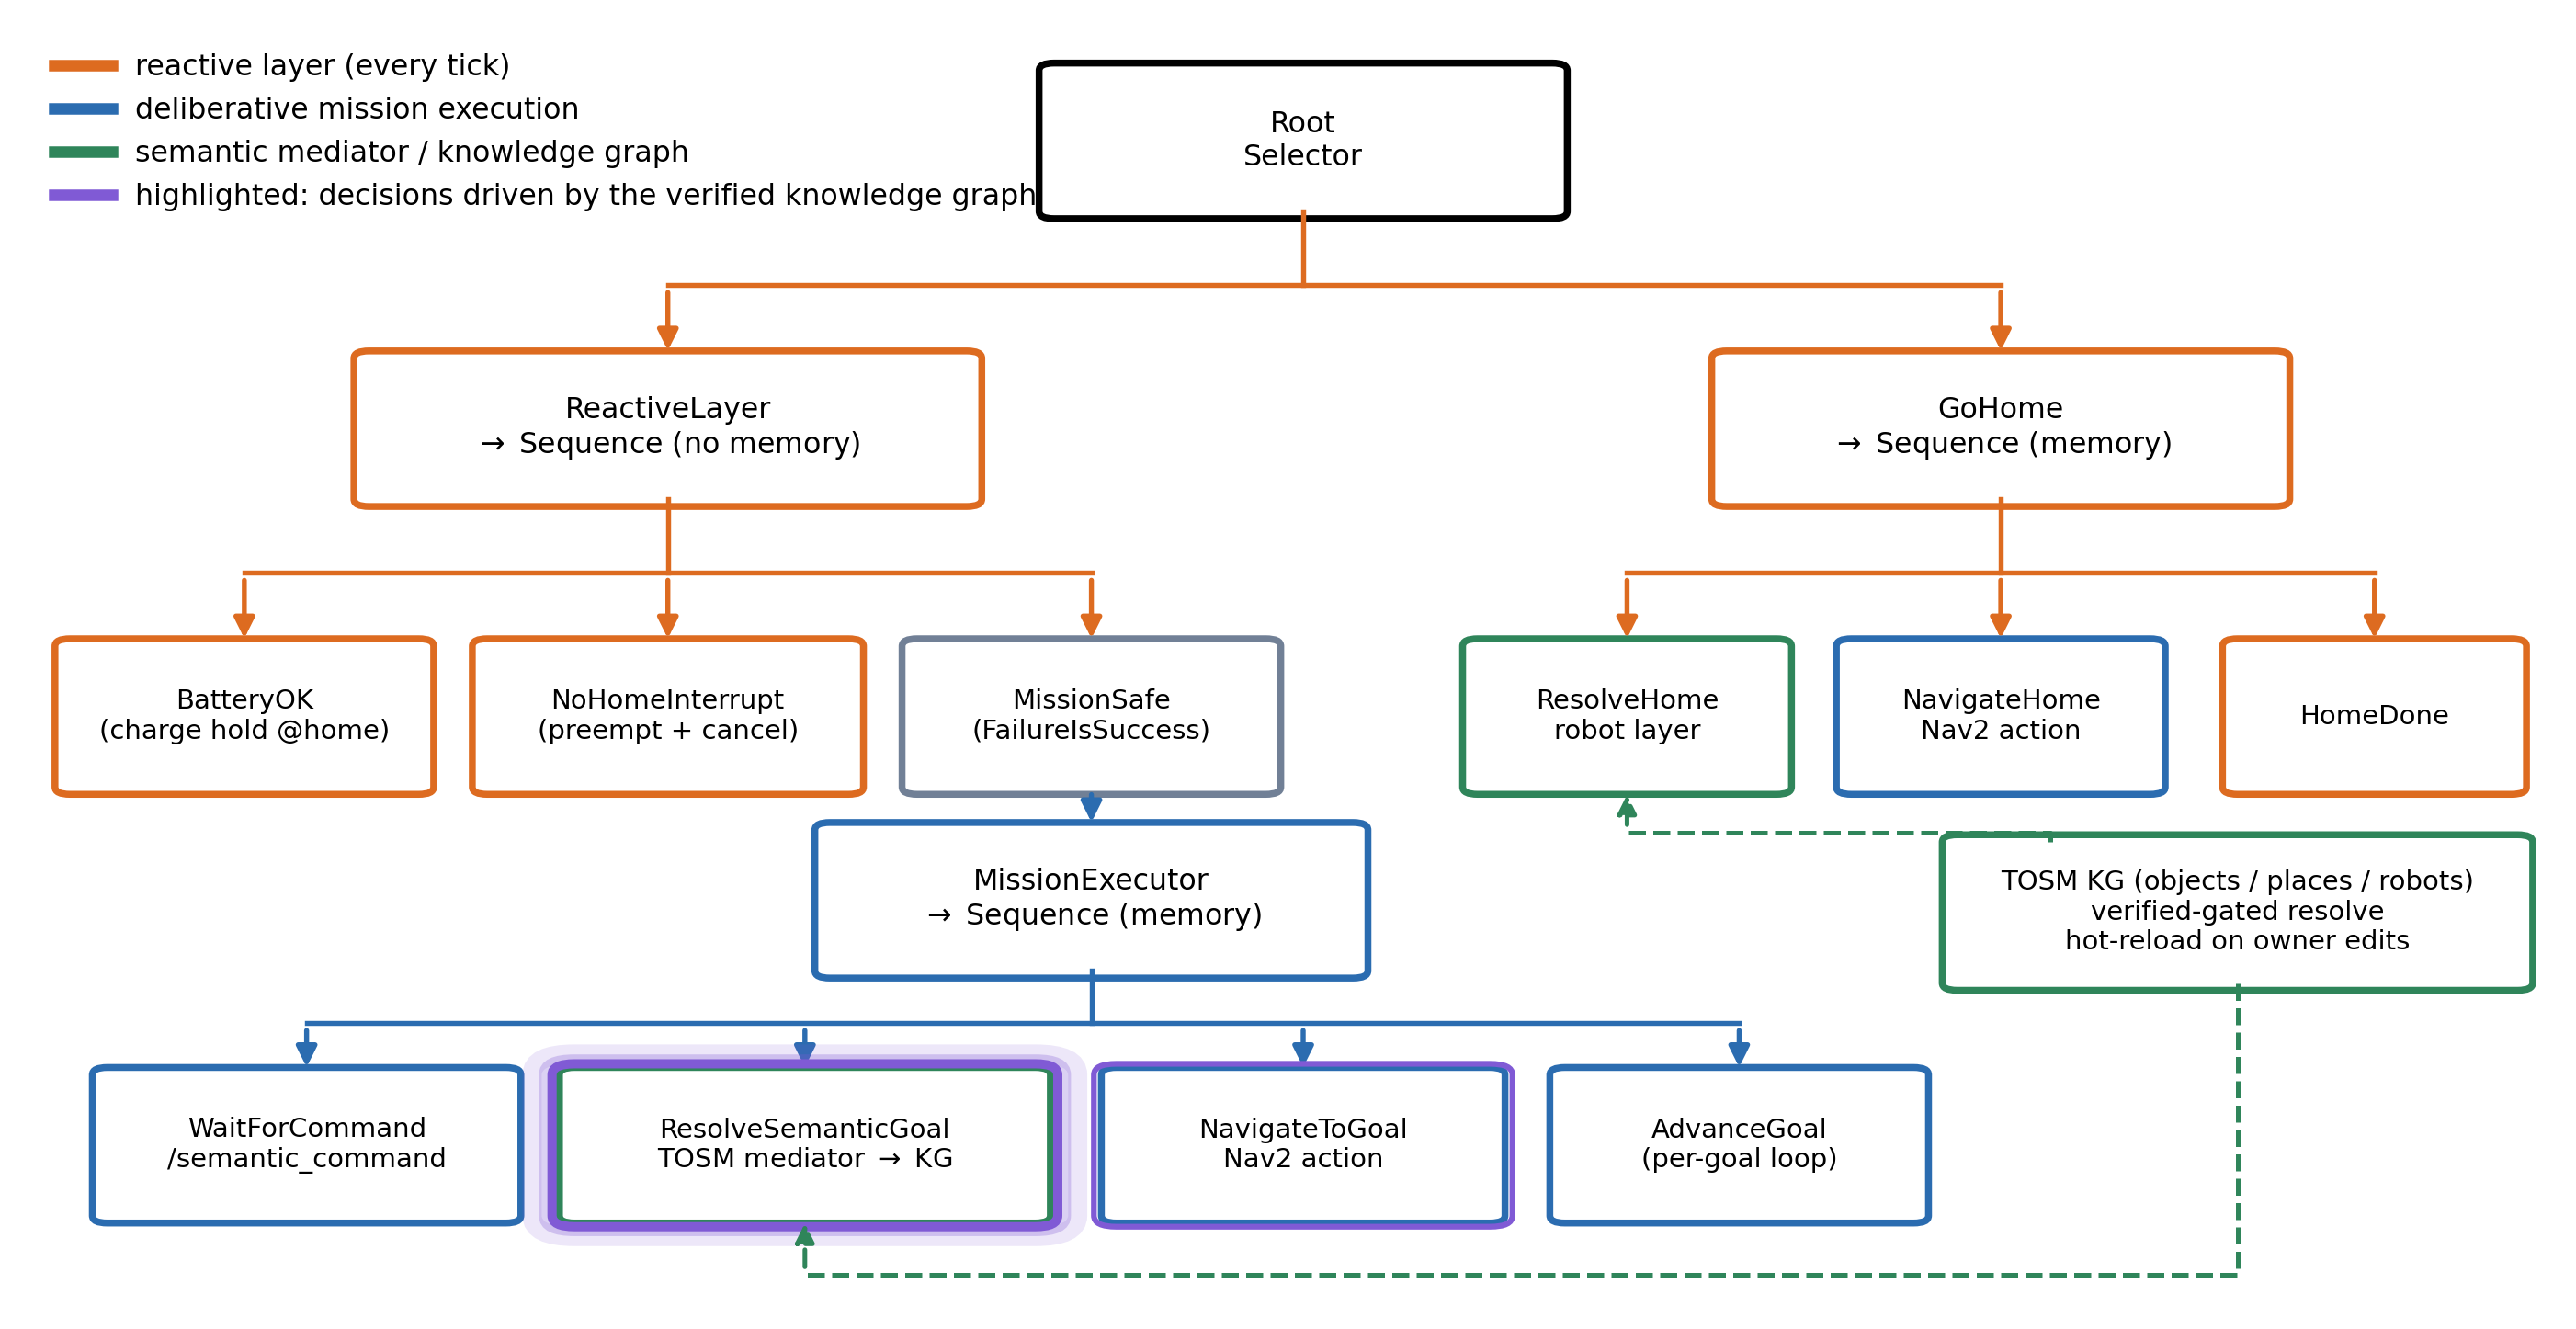
\includegraphics[width=0.9\linewidth]{figures/ele_fig16_bt_tree.png}
\caption{Hybrid deliberative/reactive mission behavior tree. The reactive
layer re-evaluates battery, stop, and interrupt conditions every tick and can
preempt navigation (canceling the active Nav2 goal); the deliberative branch
resolves semantic commands through the TOSM mediator, which hot-reloads the
knowledge graph when the management console edits it. Highlighted nodes are
the decisions the verified knowledge graph drives: the semantic-resolve node,
where a gated graph refuses phantom or unverified goals, and the navigation
node that consumes the resolved pose.}
\label{fig:bttree}
\end{figure}

In simulation, the stack runs in a Gazebo~\cite{koenig2004gazebo} world
generated from the same exploration occupancy grid that anchors the place
layer, so world, navigation map, and knowledge graph share one frame. The
simulated vehicle is a digital proxy of the target platform: the AMMR's
footprint ($1.25\times0.8$~m), lidar mount, and velocity limits from the TOSM
robot layer are instantiated in the world, and the mediator derives approach
poses and clearance checks (circumscribed radius 0.74~m) from the same
layer---the knowledge that \emph{describes} the robot is the knowledge that
\emph{drives} it.

\section{Real-Robot Integration}
\label{sec:real-robot}

To close the loop on hardware, the mission stack of Section~\ref{sec:missions}
is run unchanged against the physical AMMR, with the knowledge graph as the
semantic store. The platform runs its own localization and Nav2 stack on an
independently built occupancy map; a thin bridge node replaces the simulator.
It converts the robot's localization pose into the scan frame through the
single SE(2) offset of Equation~\ref{eq:anchor}, calibrated once by parking the
robot on a taped start spot of known scan coordinates, and republishes it as the
pose the mediator and the twin consume; in the reverse direction it exposes
the navigation action interface the behavior tree expects, forwards the
mediator's resolved goals (scan frame) to the robot's on-board navigation in
the robot's map frame, monitors arrival within a tolerance radius with a short
settling time, and implements the console's stop command by canceling the
active mission and holding the current pose. Nothing above the bridge changes:
commands are issued from the management console, the mediator resolves and
gates them against the graph, the behavior tree executes them, and the Isaac
Sim twin mirrors the robot from the same store. Because the robot reports its
heading in its own map convention, the bridge also applies a fixed heading
offset determined during the anchoring check. The measured outcomes of this
integration---conversion time, simulation throughput, geometric fidelity,
simulator-issued goal trials, and console-issued semantic missions on the
physical robot---are reported in Sections~\ref{sec:exp-twin}
and~\ref{sec:exp-missions}.
   % Digital-Twin-Based Validation
%%=============================================================================
%% chapters/chapter6.tex — Experiments and Results (final-defense version)
%%=============================================================================
\chapter{Experiments and Results}
\label{ch:experiments}
This chapter reports the experimental design and results for the three parts
of the framework.\footnote{The results of this chapter are reported in the author's publications~\cite{iccas2026,kim2026sensors,kim2026ictc,kim2026electronics,raaicon2026}; tables and figures are reproduced from them with the source indicated.} Section~\ref{sec:setup} describes the platforms, scenes,
ground-truth protocol, and metrics. Section~\ref{sec:exp-mapping} evaluates
the automated mapping subsystem of Chapter~\ref{ch:mapping} in a controlled
simulation ablation, on hardware, and through survey-grade registration.
Sections~\ref{sec:exp-seg}--\ref{sec:exp-ablation} evaluate the semantic
modeling subsystem of Chapter~\ref{ch:semantic}: segmentation repeatability
and backbone selection, multi-view verification and escalation, the owner
audit and corrective feedback, knowledge-grounded querying, incremental update,
an end-to-end replay, and ablations including a cross-floor stress scene.
Sections~\ref{sec:exp-twin} and~\ref{sec:exp-missions} evaluate the digital
twin and the semantic mission execution of Chapter~\ref{ch:validation} in
simulation and on the physical robot. Section~\ref{sec:exp-summary} maps the
results back to the research objectives.

\section{Experimental Setup}
\label{sec:setup}

\subsection{Platforms and Software Stack}
\label{subsec:platforms}

The mapping subsystem is implemented as a set of decoupled ROS~2 (Jazzy) nodes.
A mobile base builds a 2D occupancy map online with Cartographer
SLAM~\cite{hess2016}; the frontier explorer~\cite{guler2024} selects goals and
drives the robot through the Nav2 navigation stack~\cite{macenski2020marathon}
using a sampling-based model-predictive path integral
controller~\cite{williams2016}; and the stop-and-scan sequencer applies the
placement policy of Chapter~\ref{ch:mapping}. Nav2 plans on an inflated
costmap, so every path and every scan candidate keeps the robot footprint clear
of obstacles by the inflation margin (0.70~m inflation radius with a 0.22~m
robot radius in all reported runs). The target stationary sensor is a Leica
BLK360~G1 terrestrial laser scanner; a driver connects to the physical device
over Wi-Fi and executes its full-dome scan workflow.

Two mobile platforms are used. \textbf{RedBOT04} (Figure~\ref{fig:redbot}) is
the scan platform: a four-wheeled skid-steer base (footprint $71\times49$~cm)
driven by four BLDC gearmotors, with an industrial PC main controller and an
STM32 sub-controller; a YDLiDAR TG30 provides the 2D scan for SLAM and
navigation, and the BLK360 is mounted on the deck about 0.5~m above the
floor---lower than a typical 1.5--1.8~m tripod setup, so low furniture casts
longer horizontal shadows than in a manual survey. \textbf{AMMR} is the
spatial-operation robot of Chapter~\ref{ch:validation}: a swerve-drive mobile
manipulator (body $1.24\times0.79$~m) running its own AMCL localization and
Nav2 stack on an independently built map. For the controlled coverage
evaluation, a TurtleBot3 Waffle is the mobile base in
Gazebo~\cite{koenig2004gazebo}, and the physical scanner is replaced by a mock
scanner node that reproduces the BLK360 capture-and-download timing and its
failure-and-retry behavior. The semantic modeling pipeline runs on a desktop
workstation (AMD Ryzen~9 9900X, 32~GB RAM, NVIDIA RTX PRO 4000 Blackwell
24~GB), which also hosts Isaac Sim~5.1 for the twin.

\begin{figure}[!htb]
\centering
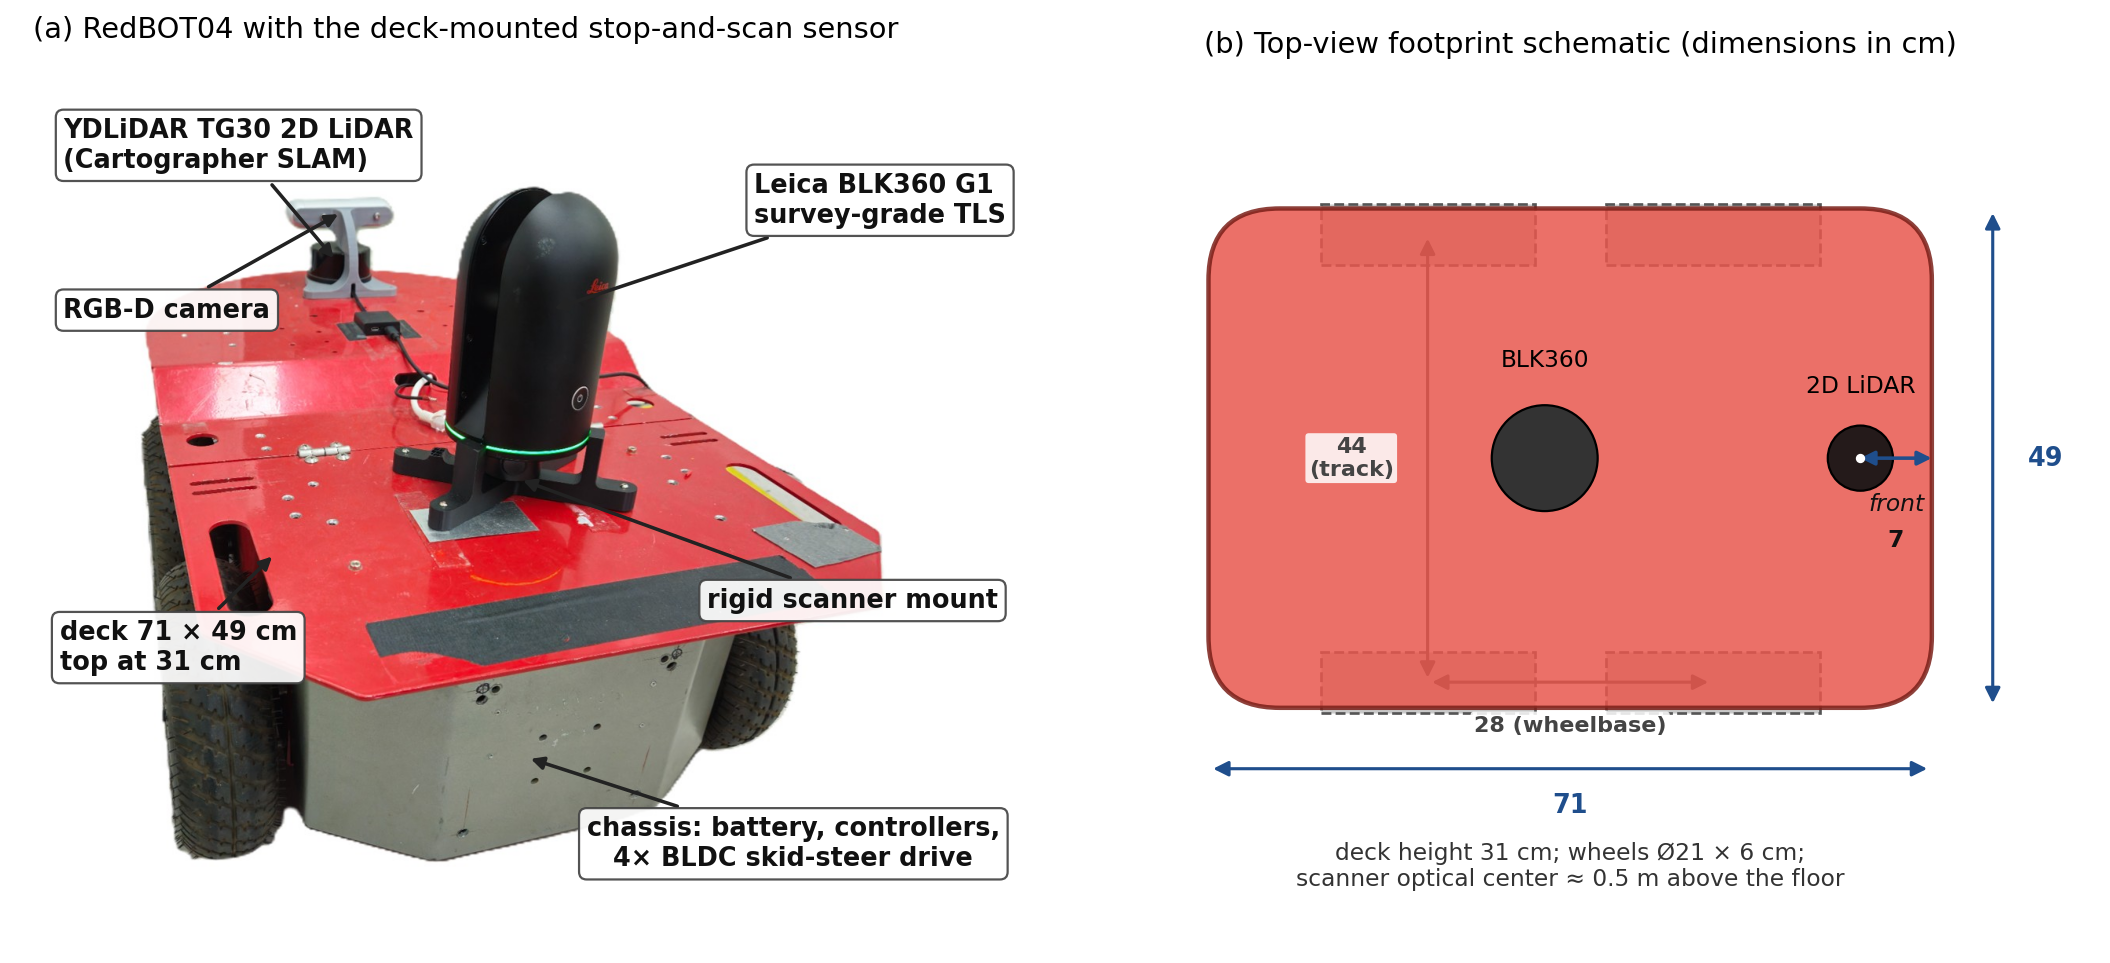
\includegraphics[width=0.9\linewidth]{figures/sen_fig9_redbot04_platform_annot.png}
\caption{RedBOT04 mobile scan platform. (a)~Annotated view with the
deck-mounted Leica BLK360~G1; (b)~top-view footprint schematic with the
principal dimensions (cm).}
\label{fig:redbot}
\end{figure}

\subsection{Environments, Scenes, and Epochs}
\label{subsec:scenes}

Two simulated indoor worlds are used for the mapping ablation. The
single-room world is generated from a real BLK360 scan of the test room,
converted to a 2D occupancy grid and extruded into a Gazebo world, so the
simulated geometry reflects the real environment
(Figure~\ref{fig:gazebo}). The multi-room world extends it with two interior
partitions and offset doorways, producing three rooms with mutual occlusion.
The physical environment for the hardware experiments and for all semantic
modeling is an \textbf{industrial test room} on the fourth floor of the
company building: an open exhibition and staging space of approximately
$13\times9$~m with a flat reflective floor, a display wall of monitors and
product panels, freestanding equipment cases, robots, and furniture that create
genuine self-occlusion (Figure~\ref{fig:testroom}); its mapped free space
spans about 105~m$^2$ on the reference map. The room combines surface types
known to stress laser-scan-based reconstruction (glass windows, dark
light-absorbing equipment, reflective flooring), it is the actual deployment
environment of the AMMR, and it allows controlled, repeatable access for the
tape-measured ground-truth campaign and the on-robot experiments.

\begin{figure}[!htb]
  \centering
  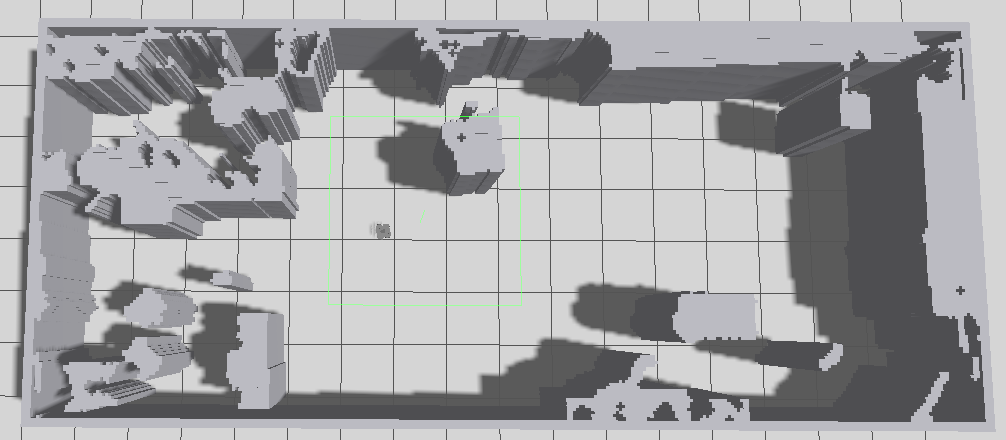
\includegraphics[width=0.85\textwidth]{figures/fig6_gazebo.png}
  \caption{The physics-based Gazebo simulation environment, built by extruding
  the 2D occupancy projection of a real survey-grade scan of the test room into
  a 3D world; the differential-drive platform explores it under the
  Cartographer/Nav2 stack.}
  \label{fig:gazebo}
\end{figure}

\begin{figure}[!htb]
\centering
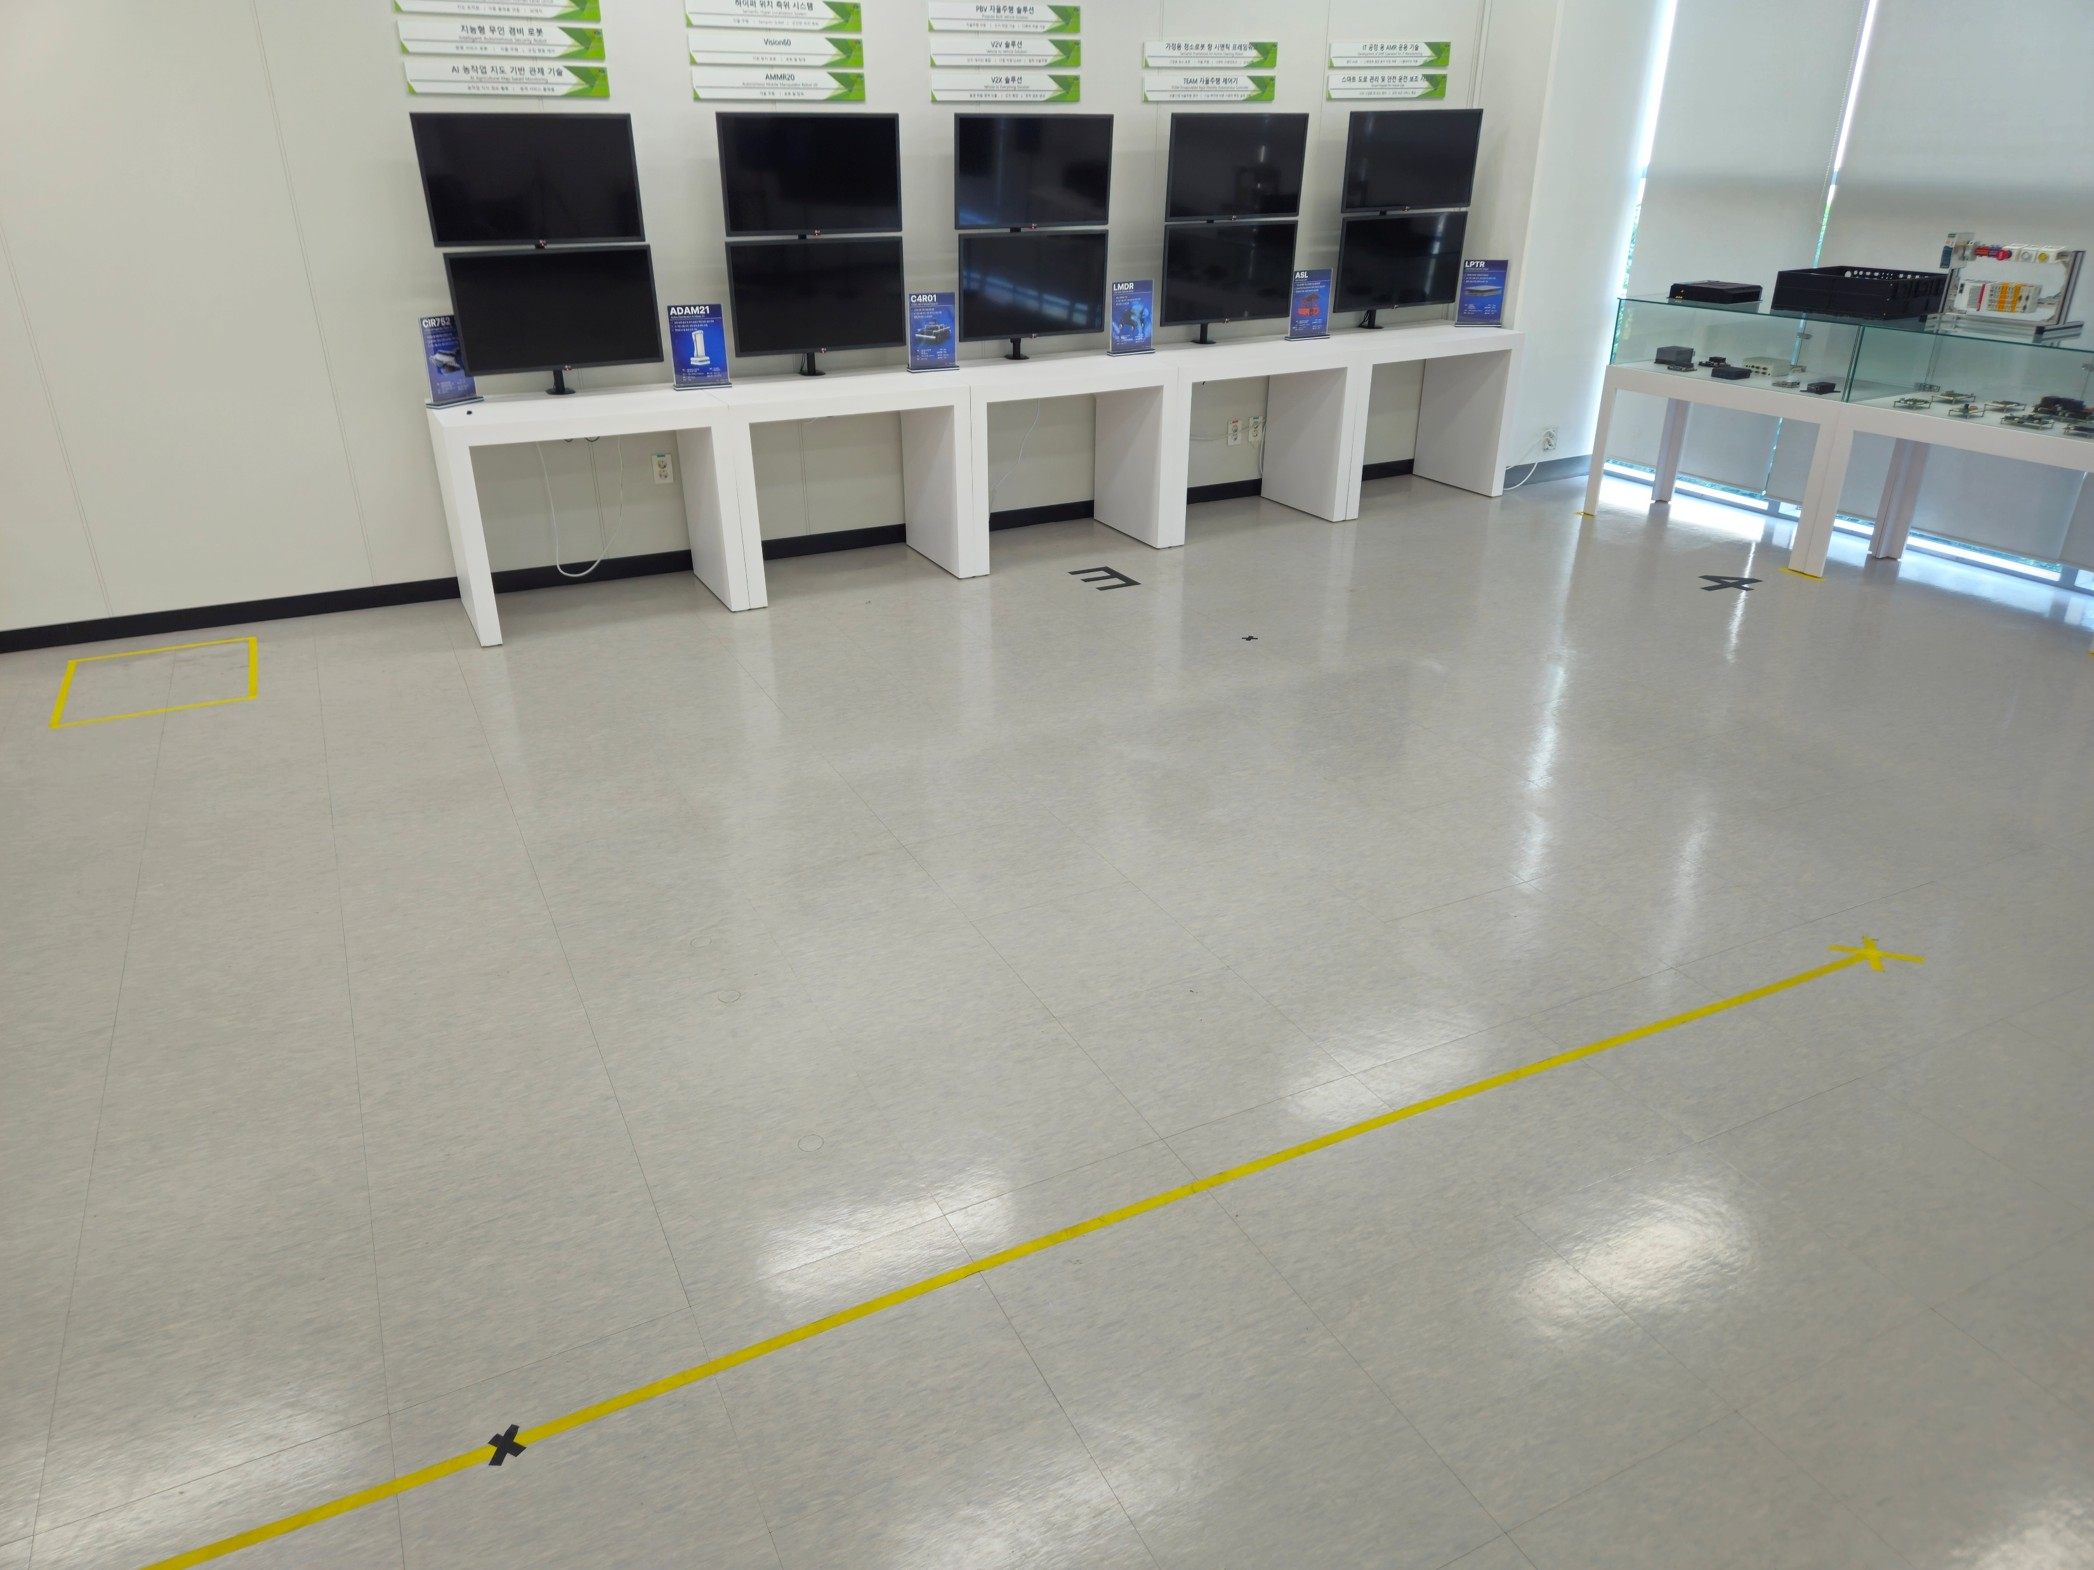
\includegraphics[width=0.9\linewidth]{figures/sen_fig10_testroom.jpg}
\caption{Physical industrial test room used for the hardware experiments and
for all semantic modeling scenes.}
\label{fig:testroom}
\end{figure}

For semantic modeling, the same room is observed across three scan epochs of
its working life, a property exploited deliberately (Table~\ref{tab:scenes},
Figure~\ref{fig:photos}). The \emph{showroom} epoch (T1, June 2026) captures
the room in an exhibition configuration, scanned manually with the door open.
The \emph{robot hall} epoch (T2, July 2026) captures the same room reorganized
as a robot test hall, scanned by autonomous visibility-driven exploration. A
third epoch (T3, late July 2026) adds a controlled-change re-scan at 99.6\%
LOS coverage. Because the two primary epochs differ in layout, furnishing, and
scan modality, they function as independent scenes for per-epoch evaluation
while enabling a real multi-epoch update study. A separate scene---a carpeted
\emph{cafeteria} with sofa booths and vending machines on the eighth floor of
the same building, scanned in August 2026 (57~M points, 28 clusters)---is held
out of the main campaign and used only as a cross-floor, out-of-vocabulary
stress case. Table~\ref{tab:sampleflow} connects every cluster set used in
this chapter to its derivation stage.

\begin{figure}[!htb]
\centering
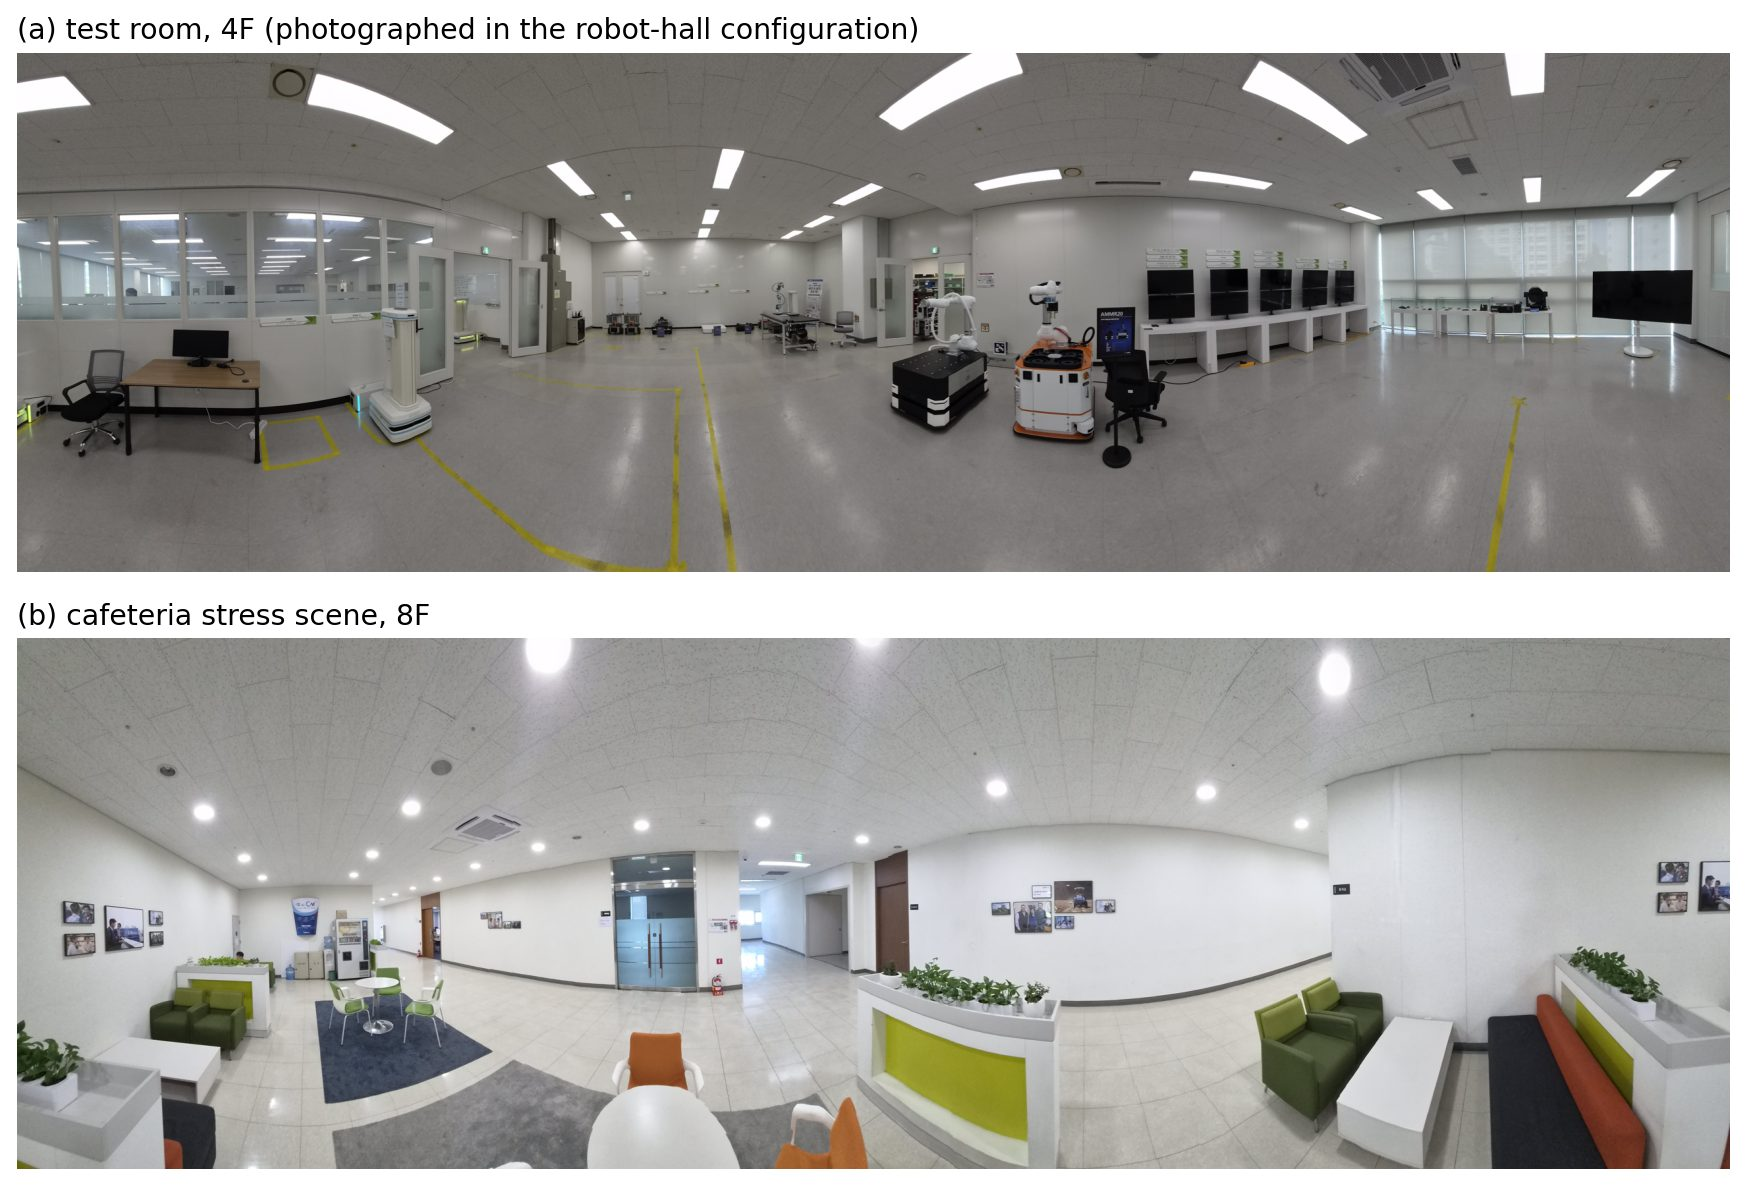
\includegraphics[width=\linewidth]{figures/ele_fig18_scene_photos.jpg}
\caption{The two semantic-modeling sites. (a)~The 4F test room in its
robot-hall configuration (T1 is an earlier furnishing of the same room;
visible: the AMMR platforms, the wall-mounted monitor bank, and a disinfection
robot). (b)~The 8F cafeteria stress scene: fabric sofas, planter partitions,
the vending row, and the brown door recovered by escalation on full-resolution
renders.}
\label{fig:photos}
\end{figure}

\begin{table}[htbp]
\centering
\caption{Scene statistics (deterministic detection sets after
structure-remnant filtering). T1 semantic processing starts from a manually
wall-removed export (4.9~M points) of the 46.3~M-point raw scan.}
\label{tab:scenes}
\small
\begin{tabularx}{\textwidth}{X c c c}
\toprule
 & \textbf{Showroom (T1)} & \textbf{Robot hall (T2)} & \textbf{Re-scan (T3)} \\
\midrule
Scan mode & manual, 1 setup & exploration & exploration, 6 setups \\
Raw points & 46.3M & 68.6M & 70.2M \\
Clean cloud (post-removal) & --- & 267K & 294K \\
Objects (filtered) & 38 & 81 & 79 \\
Room-scoped & 38 & 55 & 41 \\
Removed planes & 10 & 10 & 10 \\
\bottomrule
\end{tabularx}
\end{table}

\begin{table}[htbp]
\centering
\caption{Evaluation-set lineage: how every cluster set used in this chapter
derives from its scan ($\dagger$: grounded only in the experiment log;
``conf.''\,=\,ground-truth confirmed).}
\label{tab:sampleflow}
\small\setstretch{1.15}
\begin{tabularx}{\textwidth}{l X}
\toprule
\textbf{Lineage} & \textbf{Stage flow (cluster counts)} \\
\midrule
Showroom 57-set (Section~\ref{sec:exp-verify}) & 30 pre-split $\rightarrow$ 57 split $\rightarrow$ 50 after soffit filter $\rightarrow$ 50 GT-scored (36 conf.) \\
Showroom det set & 45 raw $\rightarrow$ 38 after soffit filter $\rightarrow$ 38 room-scoped \\
Robot hall det & 88 raw $\rightarrow$ 81 filtered $\rightarrow$ 55 room-scoped $\rightarrow$ 51 GT-scored (32 conf.) \\
T3 det1 & 79 merged $\rightarrow$ 41 room-scoped (= owner audit set) $\rightarrow$ 26 filter survivors \\
T3 det2 (precut) & 66 $\rightarrow$ 35 room-scoped $\rightarrow$ 27 to VLM (8 wall sheets excluded) \\
T3 det3/det4 & 33 consolidated $\rightarrow$ 46$^{\dagger}$ adjudicated \\
Cross-epoch KG (present) & rev7$\rightarrow$14: 47, 49, 51, 63, 64, 64, 46, \textbf{46} (current) \\
Frozen re-run (Section~\ref{sec:exp-endtoend}) & 66 $\rightarrow$ 35 in-room, scored vs.\ the 46-object graph \\
Cafeteria 8F & 28 $\rightarrow$ 25 GT-scored (20 conf.) \\
\bottomrule
\end{tabularx}
\end{table}

\subsection{Ground Truth and Annotation Protocol}
\label{subsec:gt}

Ground truth for semantic modeling was established in two passes: a
render-based audit of every cluster, followed by confirmation from the room's
owner (the facility operator) by physical inspection. Labels are graded
\emph{confirmed} (owner-verified), \emph{plausible}, or \emph{unknown};
accuracy is reported against confirmed ground truth (with lenient variants
including plausible where stated), unknown objects are excluded, and structure
artifacts are tracked separately. The showroom verification study uses the
original 57-cluster decomposition, of which 50 are scored after excluding 7
structure artifacts (confirmed 36 / plausible 12 / unknown 2); the room-scoped
robot hall has 51 scored clusters (confirmed 32); the cafeteria has 25 of 28
(confirmed 20). Both audit passes share an anchoring channel---the render
audit presents proposed labels that the owner then corrects---so confirmed
grades are owner decisions over physically known rooms rather than blind
annotations. To measure this bias directly, two blind annotations were added.
A co-author familiar with the facility who had seen neither the T3 pipeline
output nor the owner audit labeled all 41 T3 clusters blind from
full-resolution multi-view render sheets carrying only shuffled identifiers:
on the 33 clusters both annotators labeled, the blind labels agree with the
owner's on 31 (93.9\%), and on the clusters where the owner had overturned the
pipeline label the blind annotator independently reproduced the override on 25
of the 26 scored. An external annotator with no connection to the work and
no familiarity with the facility labeled the same 41 sheets under the same
protocol: without site knowledge, agreement with the owner drops to 21 of 33
(63.6\%), but 16 of 19 labels given at confidence 4--5 agree (84\%), and 11 of
the 12 disagreements fall on absorbed or merged industrial objects and on
ceiling or wall remnants---the categories that required on-site knowledge in
the owner audit. The owner ground truth is therefore described as
anchoring-bounded rather than anchoring-free. For the mapping subsystem, a
ground-truth occupancy map of the simulated test room is maintained for
map-quality registration, and tape measurements provide the reference for the
twin's geometric fidelity.

\subsection{Metrics}
\label{subsec:metrics}

Table~\ref{tab:metrics} aligns the metrics with the five research objectives
of Section~\ref{sec:objectives}. For mapping (O1), the figure of merit is LOS
coverage (Equation~\ref{eq:los}); because each autonomous run maps a slightly
different extent of free space, every cross-run comparison re-evaluates all
runs on a single common reference map (the most complete map among the runs
compared) so that all runs share the same free-space denominator, and the scan
count is reported alongside as the cost term. Registration quality is measured
by the number of setups and links, the overall overlap, and the bundle error
reported by the registration software. For the backbone (O2), repeatability is hash-verified
byte identity of clusters, and instance quality is recall against an
owner-audited inventory in a membership-independent form. For verification
(O3), classification accuracy is top-1 against confirmed ground truth under
documented synonym-tolerant matching, and verification quality is per-tier
precision, recall, and $F_1$. For querying, a \emph{hallucination} is an
unsupported atomic factual claim, and the hallucination rate is the fraction
of unsupported claims over all factual claims. Update quality uses matching accuracy, identity-switch rate,
false-new and false-absent counts, and unchanged stability. For the twin and
missions (O4, O5), conversion time, simulation throughput, tape-measured scene
dimensions and checkpoint distances, and mission success, completion time, and
arrival error are reported.

\begin{table}[htbp]
  \centering
  \caption{Evaluation metrics aligned with the five research objectives.}
  \label{tab:metrics}
  \begin{tabularx}{\textwidth}{l X X}
    \toprule
    \textbf{Objective} & \textbf{Metric} & \textbf{Section} \\
    \midrule
    O1 & LOS coverage vs.\ scan count; registration setups/links/overlap/bundle error & \ref{sec:exp-mapping} \\
    O2 & Byte-identical repeatability; instance recall vs.\ owner inventory; proxy comparison vs.\ learned baselines & \ref{sec:exp-seg} \\
    O3 & Verification accuracy, per-tier precision/recall/$F_1$; query accuracy, hallucination rate, traps blocked; matching accuracy, identity switches; automated recall & \ref{sec:exp-verify}--\ref{sec:exp-ablation} \\
    O4 & Conversion time, scene complexity, simulation throughput, dimensional error, twin positioning error & \ref{sec:exp-twin} \\
    O5 & Mission success, completion time, arrival error, phantom-goal refusal & \ref{sec:exp-missions} \\
    \bottomrule
  \end{tabularx}
\end{table}

\paragraph{Controls and generative-AI use.}
The verifier for the main semantic campaign is fixed to a single model
(Claude Sonnet~4.6~\cite{anthropic2026}); every verification, escalation, and
owner interaction in the accumulated knowledge-graph lineage was produced under
this one verifier, so results remain comparable across sections. All query
conditions share the same LLM, system prompt, query set, decoding parameters,
and forced answer schema and differ only in the knowledge view they receive.
Constants in the base pipeline were fixed on T1/T2 and applied unchanged to T3
and the cafeteria; the corrective-layer thresholds were developed on the
test-room lineage and frozen before evaluation on the cafeteria. Generative
models enter this work in two strictly separated roles: as experimental
components under test (Stage-B verification, query answering, place naming,
and the five-verifier comparison), every call made under a forced schema with
prompts and usage archived; and as a writing aid for language editing of the
underlying manuscripts, with no role in study design, data collection, or
analysis.

\section{Automated Mapping Subsystem}
\label{sec:exp-mapping}

\subsection{Scan-Trigger Strategies in the Simulated Test Room}
\label{subsec:prelim-mapping}

The first experiment, carried over from the preliminary defense, establishes
why the scan/skip decision needs a coverage model at all. Two strategies are
contrasted in the simulated test room: a \emph{distance-traveled} trigger,
which fires a stationary survey scan whenever the platform has driven a fixed
path distance with no redundancy check, and the \emph{prior-scan-radius}
strategy of Section~\ref{subsec:proximity-rule}, which proposes a candidate at
the same interval but skips any candidate within straight-line distance $R$ of
an existing scan. Five configurations are compared (Table~\ref{tab:ablation0}):
the distance-traveled baseline, three settings sweeping $R$ from 3 to 5~m, and
one with frontier suppression disabled. The distance-traveled baseline stops
21 times to map the room; the prior-scan-radius strategy maps the same room
with three scans---a roughly seven-fold reduction in expensive stationary
acquisitions---by skipping the 21 to 27 candidates that fall within $R$ of an
existing scan. Sweeping $R$ trades scan count and travel time against room
coverage, and $R=4$~m, set with reference to the scanner's effective range, was
selected. Across every configuration the free-space IoU of the resulting
Cartographer map stays between 0.94 and 0.97 with a wall RMSE near 0.31~m:
because the 2D map is built continuously from the navigation laser while the
stationary survey scans serve the dense 3D capture, reducing the number of
stops does not degrade the navigation map (Figures~\ref{fig:mapscan}
and~\ref{fig:mapqual}). Disabling frontier suppression lowers the IoU slightly
because abandoned frontiers are reapproached and inject minor drift. The
sequencer also behaves correctly under the survey-scanner timing model:
in-place rotation does not trigger scans, the capture--download decoupling lets
the platform resume motion during background downloads without overlapping
acquisitions, and the reconnect path recovers from simulated connection losses
up to the configured retry bound.

\begin{table}[htbp]
  \centering
  \caption{Scan-triggering strategies in the simulated test room
  (ground-truth free area 85.5~m$^2$; room coverage = fraction of free area
  within straight-line distance $R$ of some scan; overlap =
  $1-A_{\mathrm{cov}}/A_{\mathrm{sum}}$ over disks of radius $R$). Source:
  ICCAS~2026~\cite{iccas2026}.}
  \label{tab:ablation0}
  \footnotesize\setstretch{1.15}
  \begin{tabularx}{\textwidth}{X c c r r r r r r}
    \toprule
    \textbf{Strategy} & $R$ (m) & Supp. & Scans & Skip. & Time (s) & Overlap & Room (\%) & IoU$_{\mathrm{free}}$ \\
    \midrule
    distance-traveled   & ---  & yes & \textbf{21} & 0  & 692 & ---   & ---   & 0.965 \\
    prior-scan $R3$   & 3.0  & yes & 5  & 21 & 416 & 0.241 & 88.2  & ---   \\
    prior-scan $R4$ (selected) & 4.0 & yes & \textbf{3} & 27 & 357 & 0.164 & 91.0 & \textbf{0.965} \\
    prior-scan $R5$   & 5.0  & yes & 3  & 22 & 309 & 0.222 & \textbf{98.9}  & 0.956 \\
    prior-scan $R4$, no supp. & 4.0 & no & 3 & 24 & 339 & 0.166 & 93.6 & 0.938 \\
    \bottomrule
  \end{tabularx}
\end{table}

\begin{figure}[!htb]
  \centering
  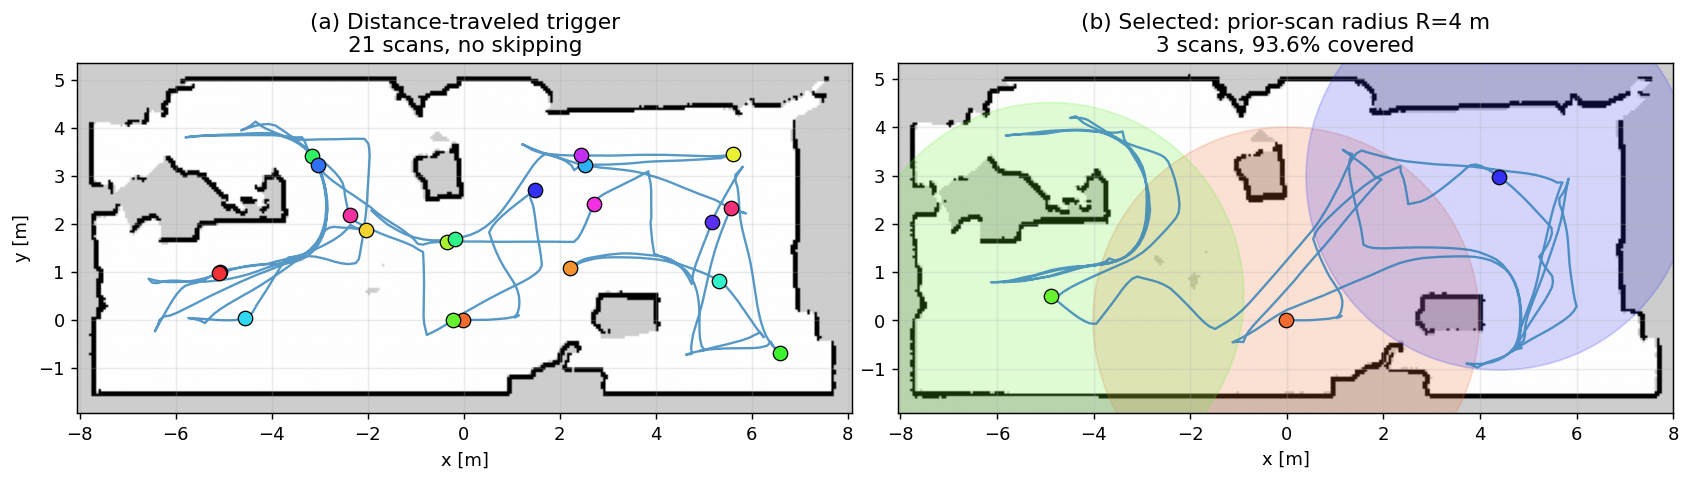
\includegraphics[width=\textwidth]{figures/fig6_strategy.png}
  \caption{Scan-triggering strategies overlaid on the Cartographer SLAM map
  (shaded disks: the skip radius $R$ around each scan; solid line: the robot
  trajectory; markers: scan positions). (a)~The distance-traveled trigger
  fires 21 scans. (b)~The prior-scan radius ($R=4$~m) maps the room with 3
  scans.}
  \label{fig:mapscan}
\end{figure}

\begin{figure}[!htb]
  \centering
  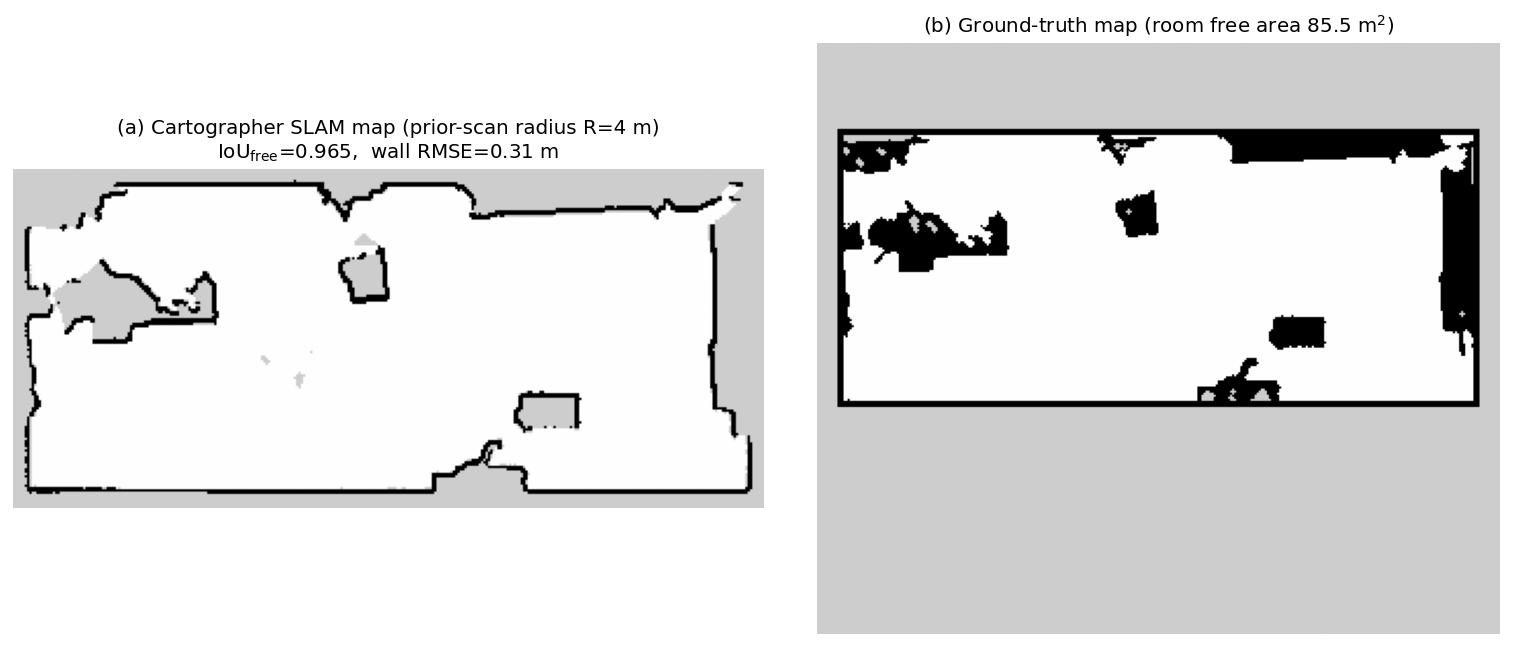
\includegraphics[width=0.92\textwidth]{figures/fig6_mapqual.png}
  \caption{Map quality of the selected run ($R=4$~m). (a)~The Cartographer
  occupancy map, $\mathrm{IoU}_{\mathrm{free}}=0.965$ and wall RMSE 0.31~m
  after translation alignment to ground truth. (b)~The ground-truth occupancy
  map of the test room.}
  \label{fig:mapqual}
\end{figure}

The proximity rule, however, judges coverage by Euclidean distance alone. The
remainder of this section evaluates the visibility-based policy of
Sections~\ref{sec:coverage} and~\ref{sec:placement} on two axes, LOS coverage
and stationary scan count. Four placement policies are compared throughout:
(i)~a \emph{uniform no-skip} reference that scans at every candidate---an
upper reference on the coverage attainable along a path; (ii)~the \emph{disk
spacing} baseline above; (iii)~the \emph{disk marginal-gain} baseline, which
applies the identical accept/skip rule as the proposed policy to the disk
coverage model; and (iv)~the proposed \emph{ray-cast visibility} policy.
Published TLS scan-planning methods are not applicable as online baselines
because they optimize viewpoints offline over a prior environment
model~\cite{tls-scanplanning,dehbi2021,knechtel2025}.

\subsection{Coverage Model and Single-Room Placement}
\label{subsec:exp-singleroom}

Figure~\ref{fig:concept} contrasted the two coverage models for a single scan
pose. On the full single-room world, the visibility stop-and-scan policy
places four scans and reaches 97.9\% LOS coverage
(Figure~\ref{fig:singleroom}). Varying the range bound $R\in\{5,6,10\}$~m
yields 97--98\% LOS in all cases (Figure~\ref{fig:rsweep}); larger $R$ needs
fewer scans but spreads them apart, reducing inter-scan overlap. $R=6$~m is
adopted for three reasons: it balances coverage against the scan-to-scan
overlap that registration benefits from; it keeps every cell claimed as
covered well inside the scanner's highest-accuracy band (3D point accuracy of
6~mm at 10~m~\cite{leica-blk360}); and it matches the local room scale, and
hence the occlusion scale, of the indoor environments targeted.

\begin{figure}[!htb]
\centering
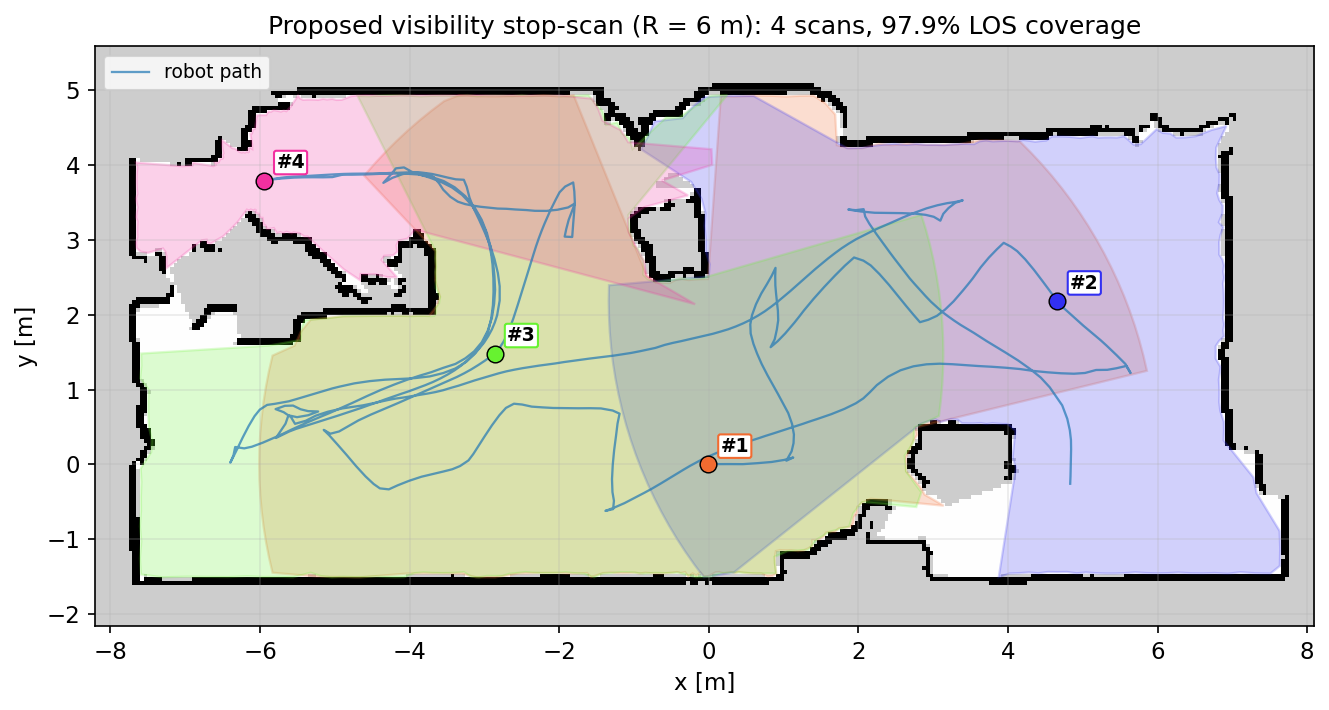
\includegraphics[width=0.7\linewidth]{figures/sen_fig2_singleroom_sota.png}
\caption{Visibility stop-and-scan on the single-room world ($R=6$~m): 4~scans,
97.9\% LOS coverage. Each accepted scan pose (marker) and its visibility
polygon share one color, indexed by scan order; the grayscale background is
the occupancy map and the blue line the robot path.}
\label{fig:singleroom}
\end{figure}

\begin{figure}[!htb]
\centering
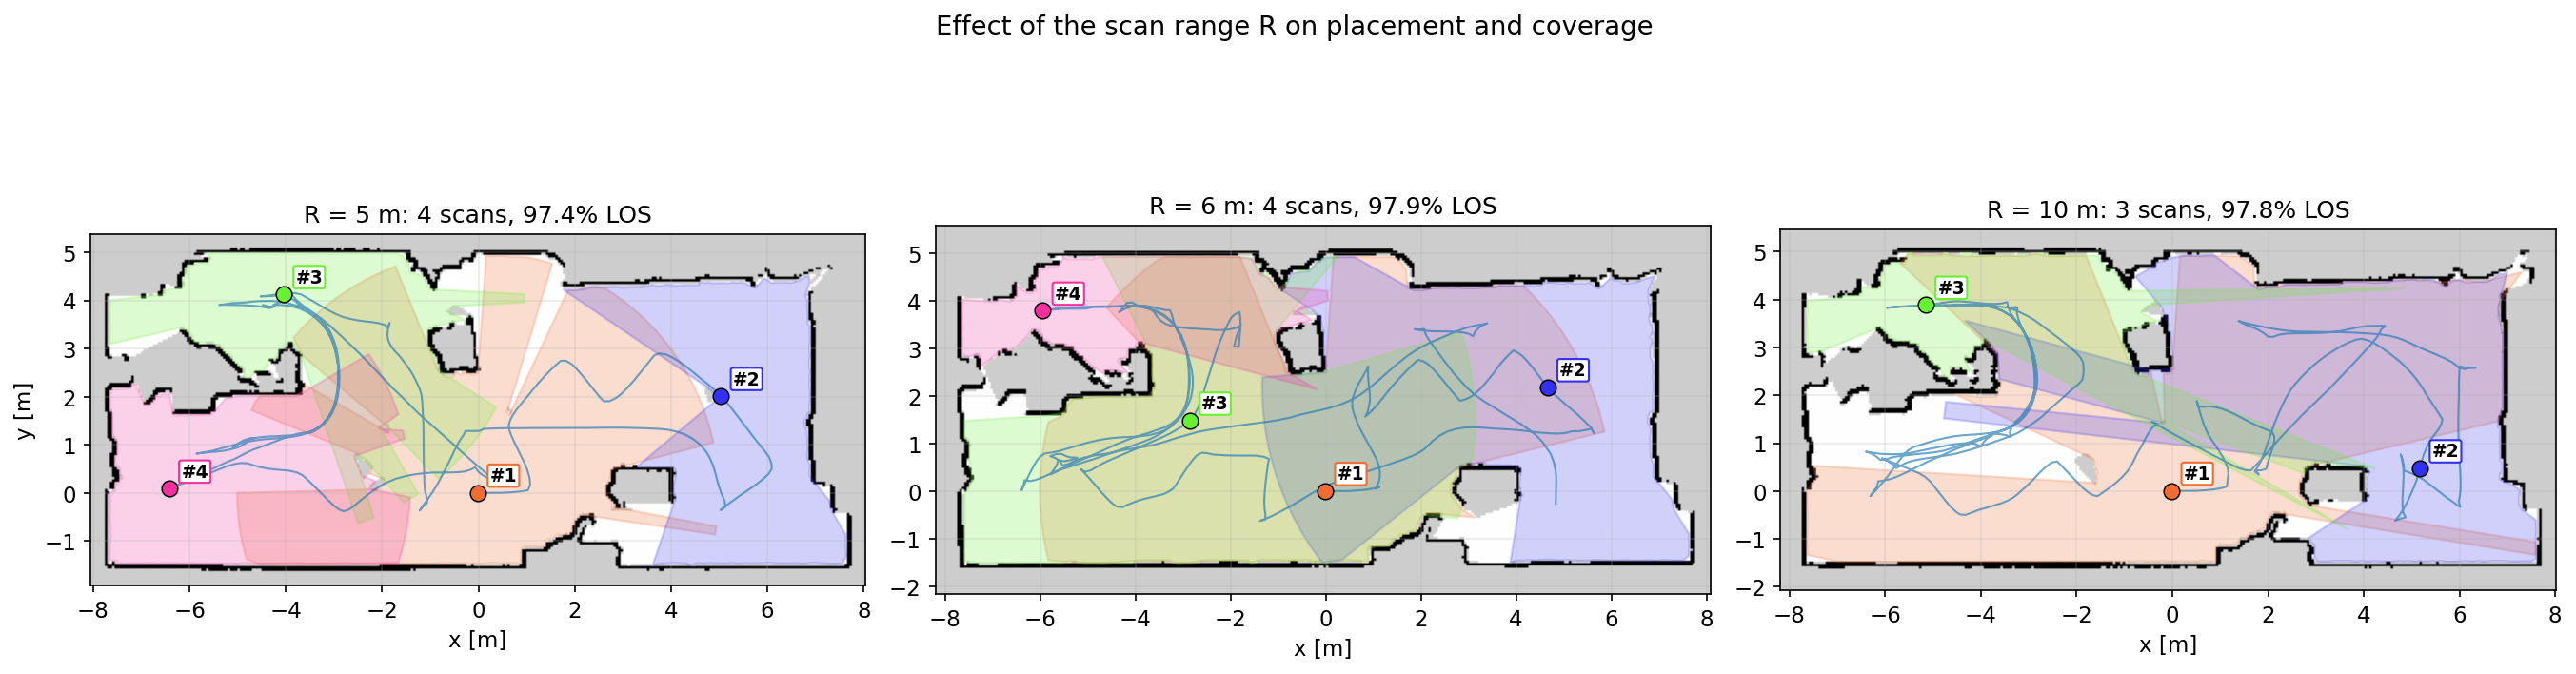
\includegraphics[width=0.95\linewidth]{figures/sen_fig3_R_sweep.png}
\caption{Effect of the range bound $R$ on placement and coverage for
$R=5/6/10$~m. Larger $R$ needs fewer scans but spreads them; $R=6$~m balances
coverage (97.9\%) against inter-scan overlap for registration.}
\label{fig:rsweep}
\end{figure}

\subsection{Controlled Skip-Rule Ablation}
\label{subsec:exp-ablation}

The decisive comparison isolates the only variable of interest, the
accept/skip decision, from the stochasticity of autonomous exploration. On a
fixed environment map and a fixed candidate sequence (a logged trajectory
resampled every 2~m of path length, denser than the live 3~m trigger so that no
policy is starved of decision opportunities), \emph{all} policies are
replayed, so they see identical maps and identical candidate poses and differ
only in which candidates they accept (Figure~\ref{fig:ablation}). This
deterministic, paired design removes the confound that, in live runs, which
rooms get mapped is dominated by navigation through narrow doorways rather
than by the skip rule.

Across $N=5$ single-room and $N=10$ multi-room trajectories, the visibility
rule raises LOS coverage from $77.0\pm4.9\%$ to $85.4\pm6.2\%$ in the
single-room world and from $77.0\pm6.4\%$ to $84.0\pm9.2\%$ in the three-room
world, at a cost of one to two additional scans on average
(Table~\ref{tab:ablation}, Figure~\ref{fig:summary}). The uniform no-skip
reference reaches $91.9\pm7.0\%$ and $86.6\pm9.9\%$ LOS, but at 28.0 and 40.8
scans on average; the visibility rule comes within 6.5 and 2.6 percentage
points of this brute-force upper reference while taking roughly an eighth as
many scans, and exceeds the disk baseline by $+8.4$ and $+7.0$ points. On
paths that traverse every room, where the disk rule's blindness to occlusion
is fully exercised, the per-path gain reaches $+21$ to $+23$ points. The disk
spacing rule is structurally capped: once two scans are placed, almost every
later candidate lies within $R$ of a prior scan, so it stops scanning even
though walls occlude much of the area it counts as covered.

The disk marginal-gain baseline isolates the coverage model from the
acceptance rule. Under the identical dual criterion, the disk model accepts
$2.6\pm0.5$ scans for $77.7\pm3.8\%$ LOS in the single-room world---essentially
the spacing rule's result---and $2.9\pm0.3$ scans for only $59.1\pm1.3\%$ LOS
in the multi-room world, markedly \emph{worse} than even the spacing rule.
Because $B_{\mathrm{disk}}$ claims area through partitions, the disk model's
own coverage bookkeeping saturates after the first few acceptances: every
later candidate appears almost fully covered, so the rule stops scanning while
whole rooms remain unobserved. That the same acceptance rule produces a
24.9-point LOS gap between the two coverage models in the multi-room world is
the sharpest form of this dissertation's claim: the deficiency lies in the
disk coverage model itself, not in the acceptance rule attached to it.

\begin{table}[htbp]
\centering
\caption{Controlled skip-rule ablation: four placement policies replayed on
the same fixed candidate sequences ($N=5$ single-room, $N=10$ multi-room
paths); mean\,$\pm$\,s.d. All policies traverse the identical path, so they
differ only in scan count. Source: \emph{Sensors}~\cite{kim2026sensors}.}
\label{tab:ablation}
\begin{tabular}{l l c c}
\toprule
\textbf{Environment} & \textbf{Coverage model} & \textbf{LOS coverage (\%)} & \textbf{Scans} \\
\midrule
\multirow{4}{*}{Single-room} & Uniform, no skip (reference) & $91.9\pm7.0$ & $28.0\pm13.0$ \\
                             & Disk, spacing rule (baseline) & $77.0\pm4.9$ & $2.0\pm0.0$ \\
                             & Disk, marginal-gain rule      & $77.7\pm3.8$ & $2.6\pm0.5$ \\
                             & Ray-cast visibility (ours)   & $\mathbf{85.4\pm6.2}$ & $3.6\pm0.9$ \\
\midrule
\multirow{4}{*}{Multi-room}  & Uniform, no skip (reference) & $86.6\pm9.9$ & $40.8\pm11.8$ \\
                             & Disk, spacing rule (baseline) & $77.0\pm6.4$ & $2.3\pm0.5$ \\
                             & Disk, marginal-gain rule      & $59.1\pm1.3$ & $2.9\pm0.3$ \\
                             & Ray-cast visibility (ours)   & $\mathbf{84.0\pm9.2}$ & $3.6\pm0.7$ \\
\bottomrule
\end{tabular}
\end{table}

\begin{figure}[!htb]
\centering
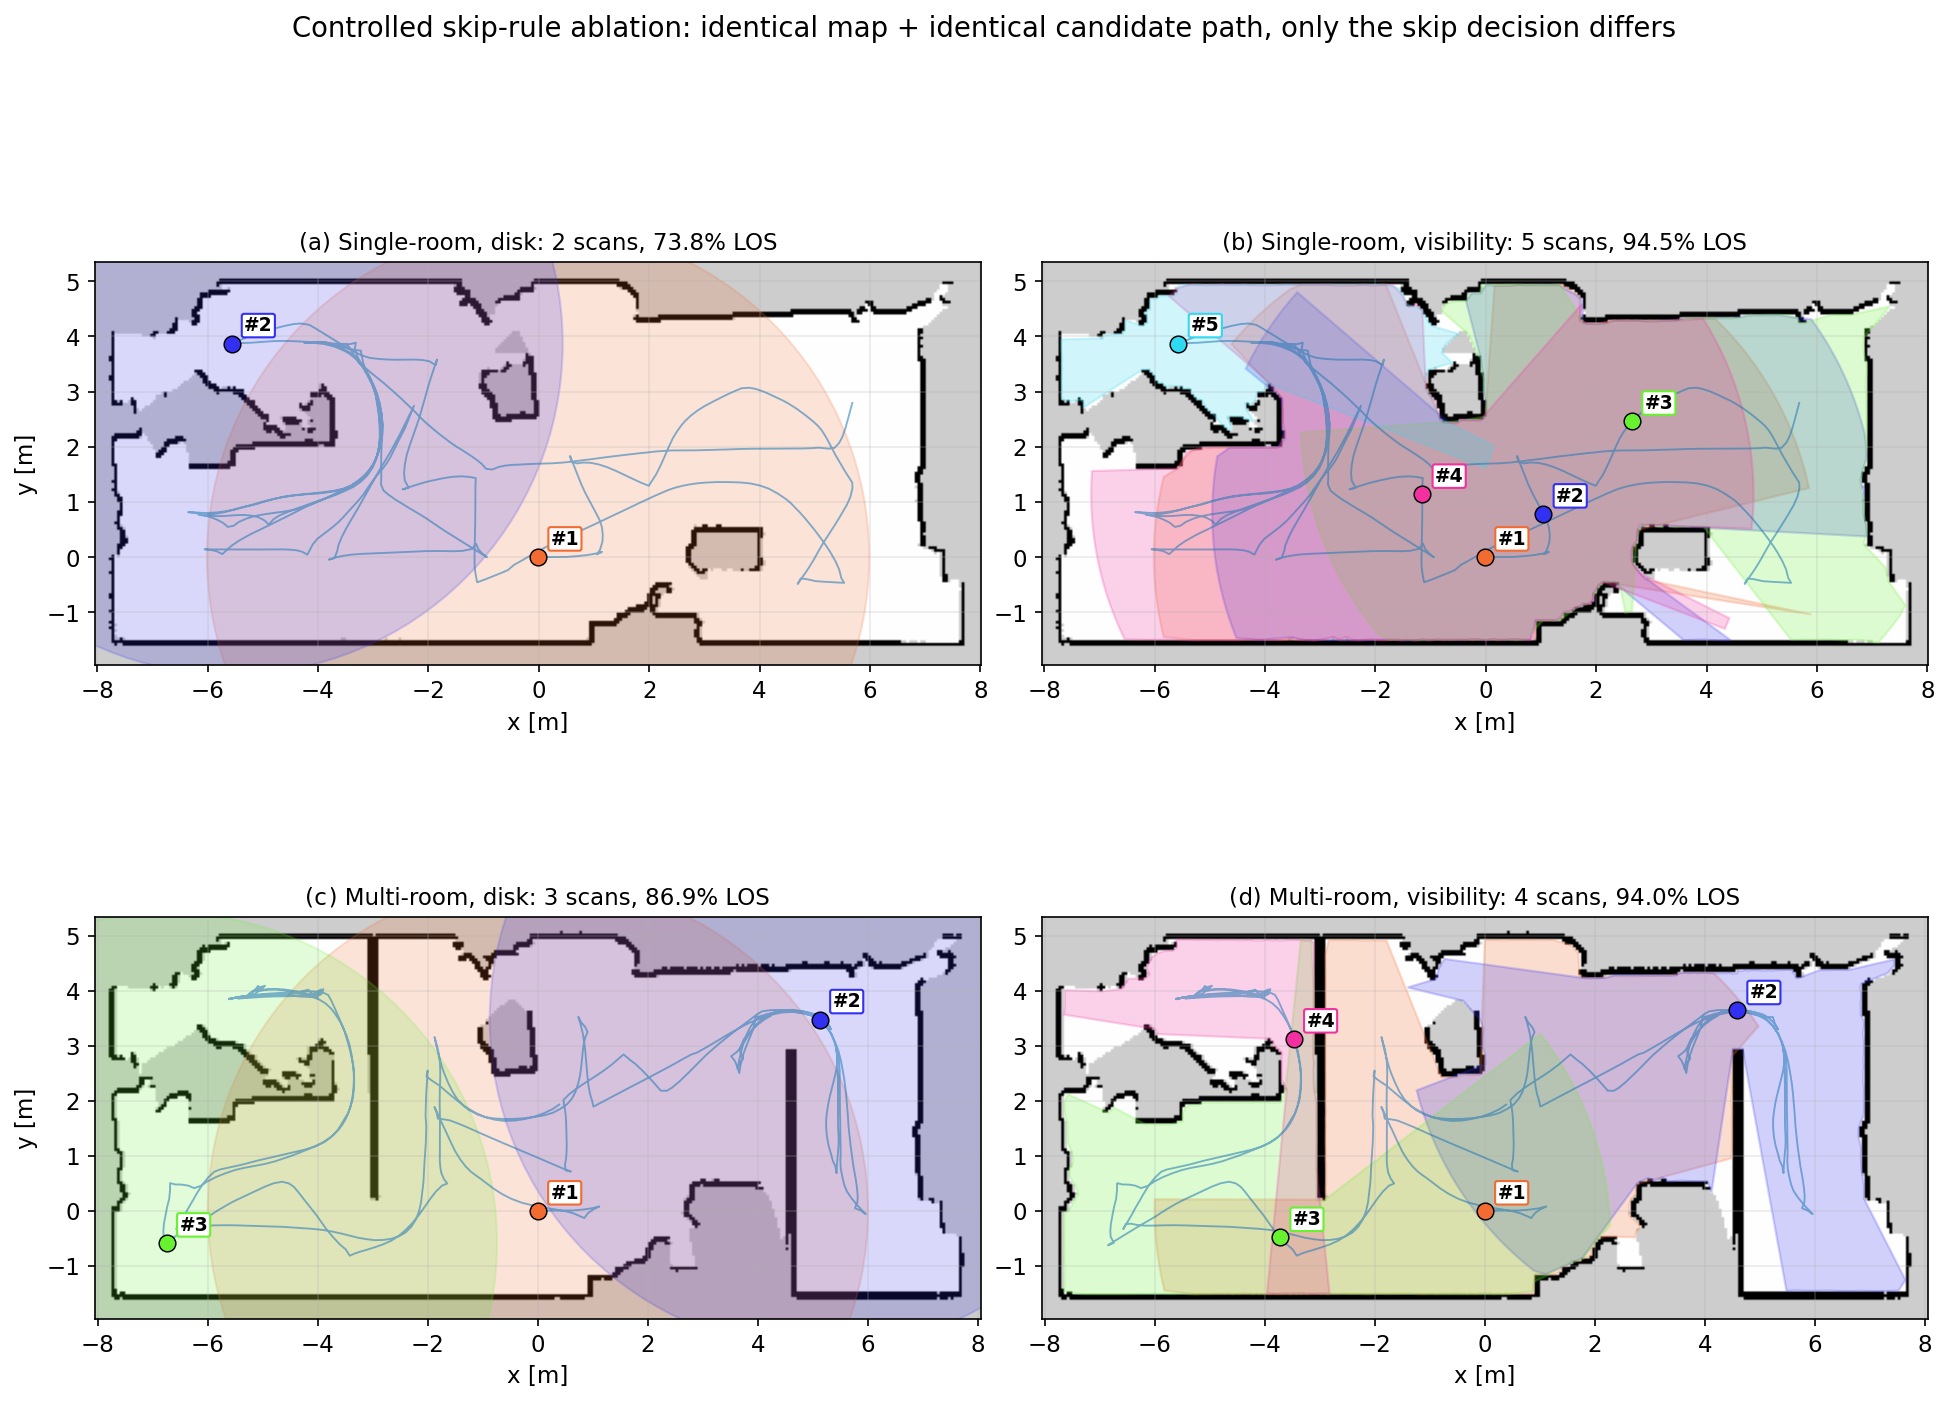
\includegraphics[width=0.95\linewidth]{figures/sen_fig5_skip_ablation.png}
\caption{Controlled skip-rule ablation on an identical map and candidate
path; only the skip decision differs. (a,b)~Single-room and (c,d)~multi-room,
under the disk spacing rule (a,c) and the visibility rule (b,d).}
\label{fig:ablation}
\end{figure}

\begin{figure}[!htb]
\centering
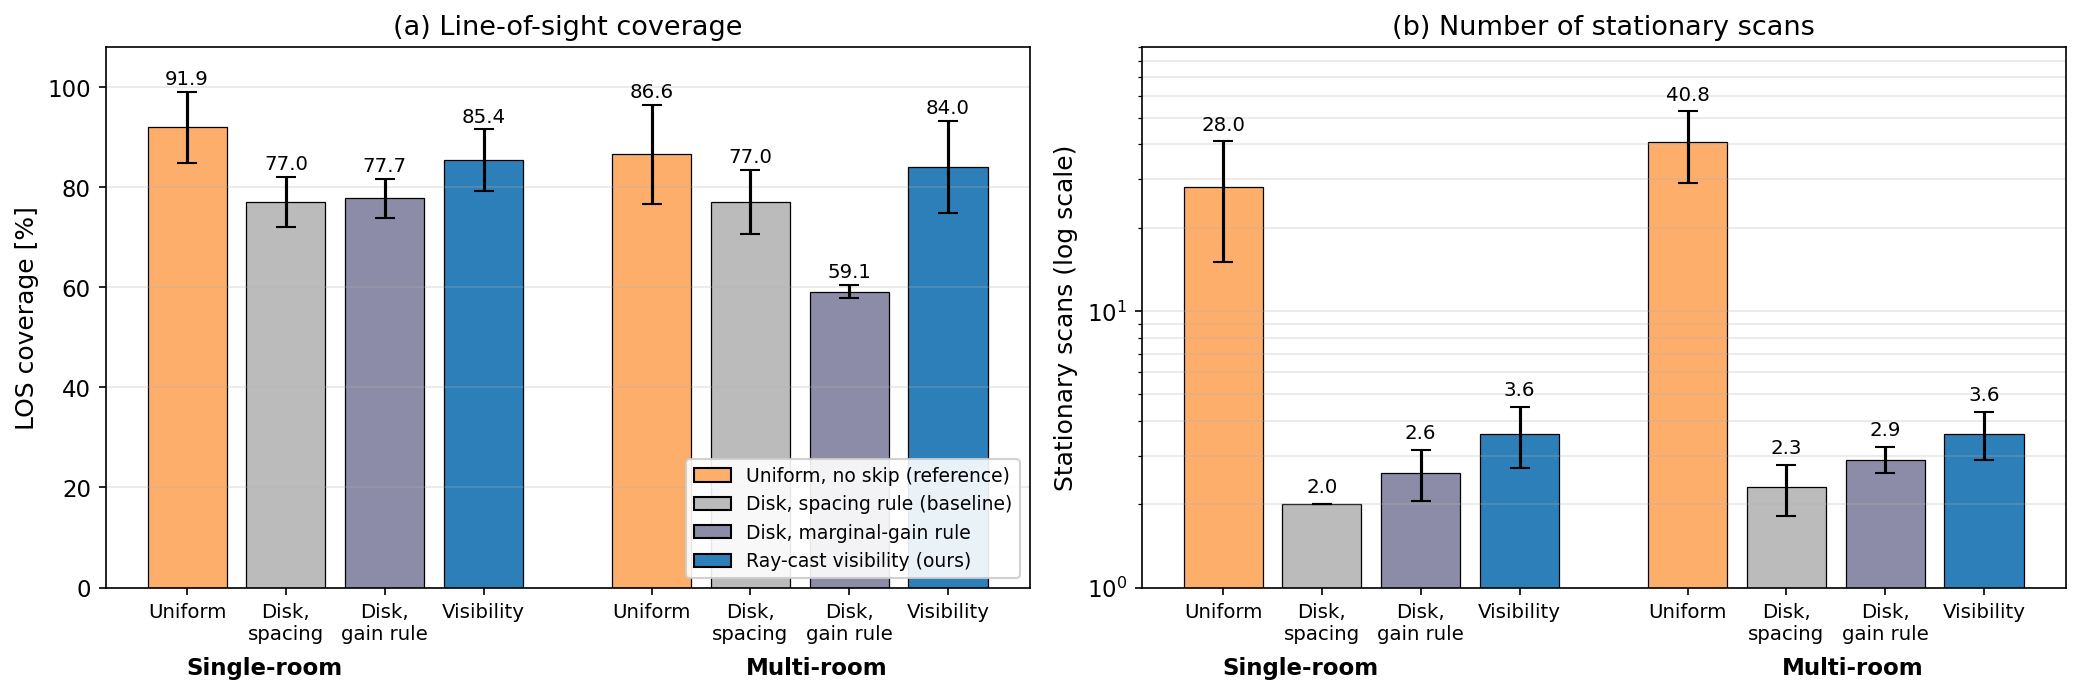
\includegraphics[width=0.95\linewidth]{figures/sen_fig7_summary.png}
\caption{Four-way skip-rule comparison on identical paths ($N=5$ single-room,
$N=10$ multi-room trajectories, paired per path). (a)~LOS coverage;
(b)~stationary scan count, log scale (mean\,$\pm$\,s.d.).}
\label{fig:summary}
\end{figure}

\subsection{Live Multi-Room Demonstration, Coverage Completion, and Parameter Sensitivity}
\label{subsec:exp-sensitivity}

Figure~\ref{fig:multiroom} shows a single live autonomous run on the
multi-room world under each coverage model. The disk policy stops after two
scans at 46.9\% LOS, having counted an entire room behind a partition as
covered through the wall; the visibility policy places one scan per room,
three in total, and reaches 95.1\% LOS. This run is presented as a qualitative
demonstration: in live runs on the partitioned world, which rooms get mapped
varies from run to run and dominates the measured coverage largely
independently of the skip rule, so the rigorous claim is the controlled
ablation above. With the coverage-completion phase enabled, the robot continues
after frontier convergence to drive into and scan the remaining uncovered
pockets: over $N=5$ runs this raises LOS coverage to $98.9\pm0.9\%$ using
$5.0\pm1.2$ total scans on average (3.2 frontier plus 1.8 completion scans),
with no unreachable pockets; a representative run reaches 99.6\% LOS
(Figure~\ref{fig:completion}).

\begin{figure}[!htb]
\centering
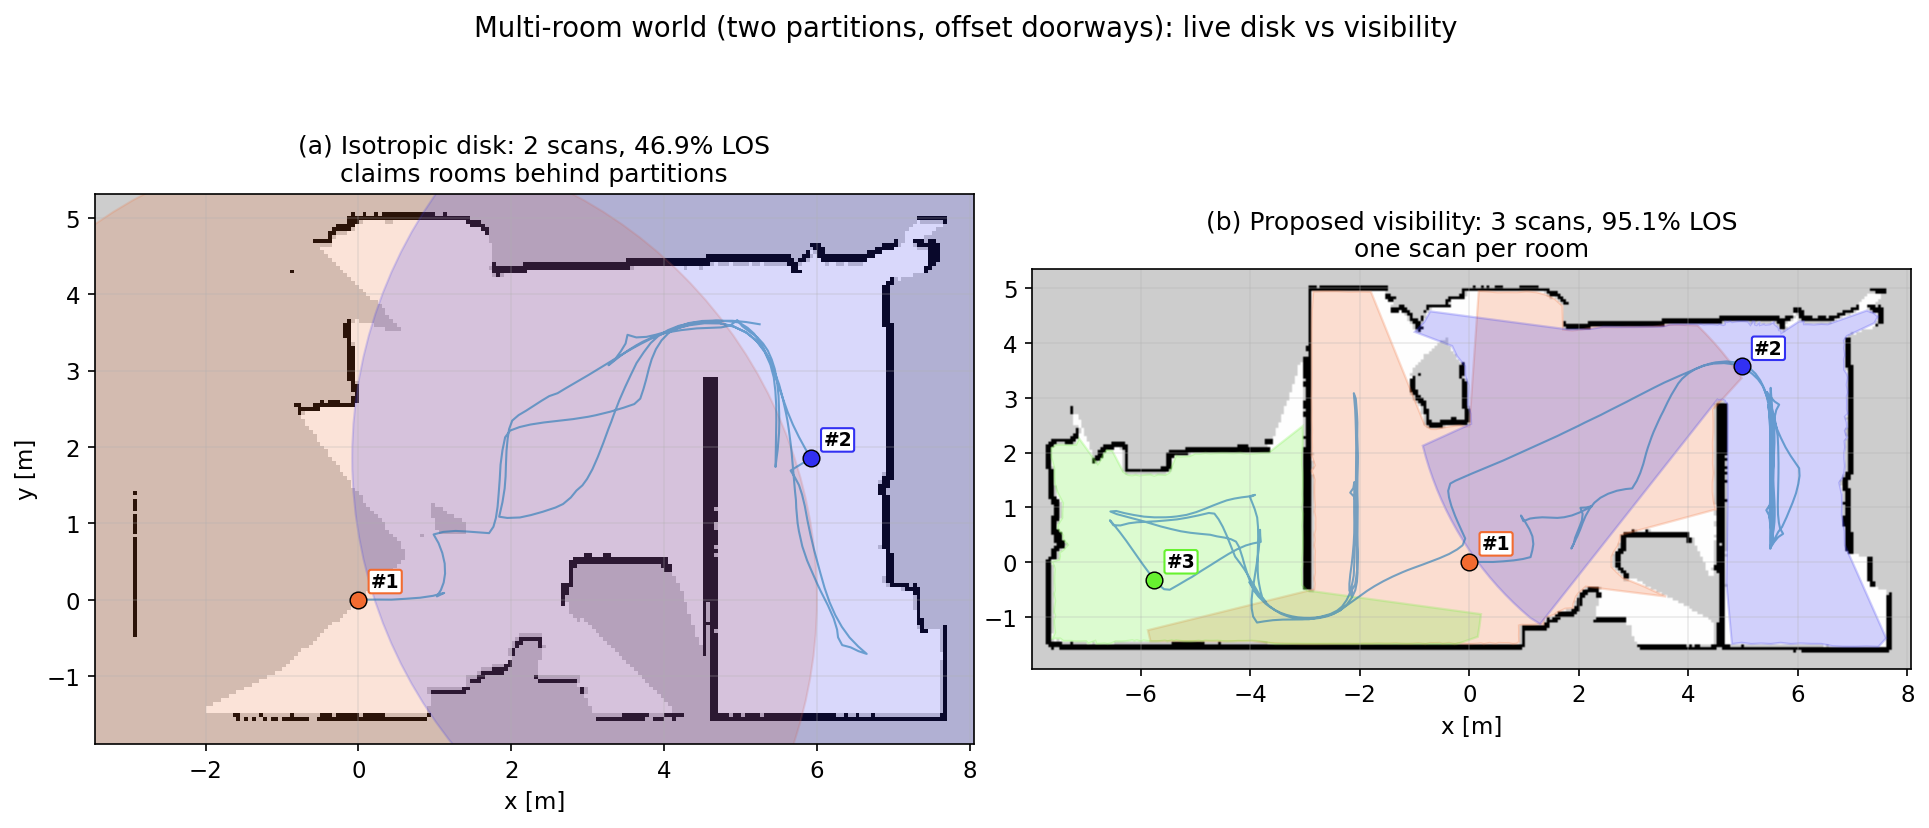
\includegraphics[width=0.95\linewidth]{figures/sen_fig4_multiroom_compare.png}
\caption{Multi-room world (two partitions, offset doorways): live disk vs.\
visibility. (a)~The disk model skips candidates within $R$ of a prior scan
through the partitions, giving 2~scans and 46.9\% LOS with a whole room
unscanned. (b)~The visibility model scans once per room, giving 3~scans and
95.1\% LOS.}
\label{fig:multiroom}
\end{figure}

\begin{figure}[!htb]
\centering
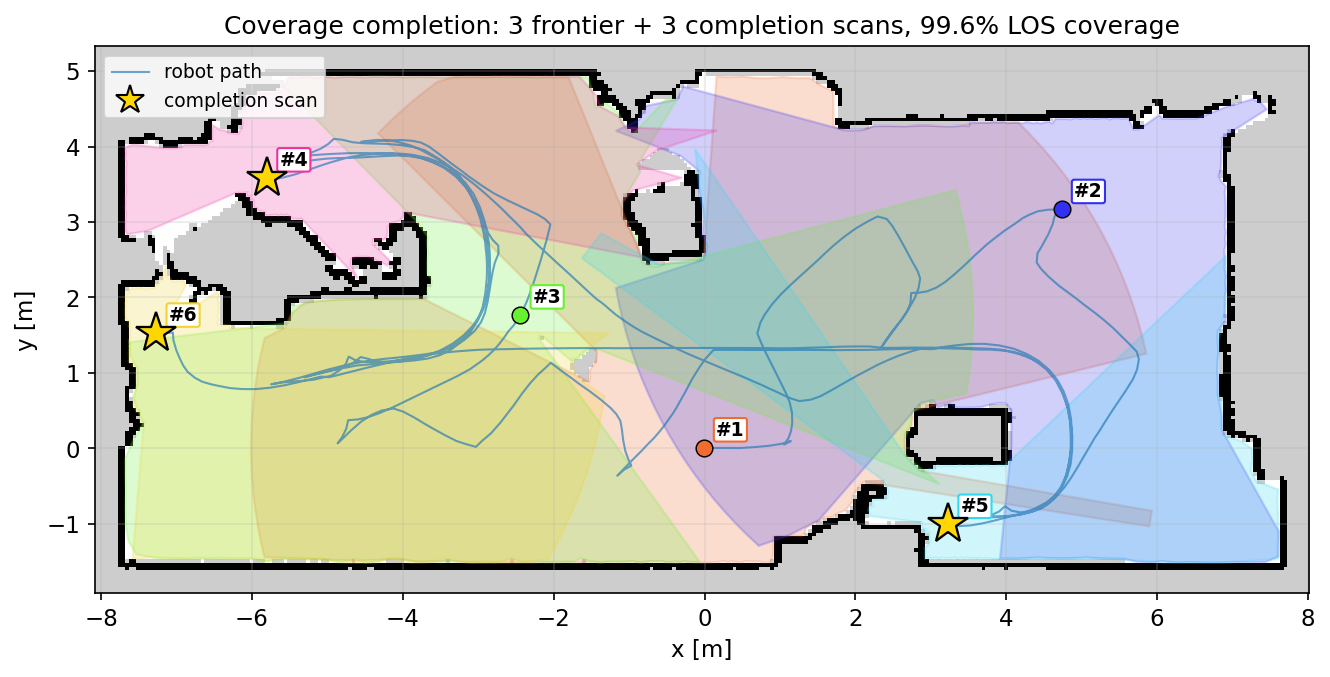
\includegraphics[width=0.7\linewidth]{figures/sen_fig6_completion.png}
\caption{Coverage completion. After frontier exploration, the robot drives
into each still-uncovered pocket and scans ($\star$) until none above the
minimum pocket area remains. Here 3~frontier $+$ 3~completion scans, 99.6\%
LOS.}
\label{fig:completion}
\end{figure}

The two skip thresholds are characterized by deterministic replay of the
visibility policy over the same fixed paths (Figure~\ref{fig:sweep}). Varying
the relative threshold $\tau$ over $[0.10,0.50]$ changes mean LOS coverage by
at most about two points (single-room $86.4\to84.3\%$; multi-room
$85.2\to84.0\%$) and mean scan count by less than one scan, so $\tau=0.30$ is
not a sensitive choice. The absolute threshold $A_{\min}$ is the operative
knob: $A_{\min}=5$~m$^2$ is the largest threshold whose mean LOS remains within
about five points of the most aggressive setting ($A_{\min}=1$~m$^2$) in both
environments (single-room 85.4 versus 90.7\%; multi-room 84.0 versus 85.7\%)
while already halving the scan count (3.6 versus 7.2 scans). Beyond the knee
the trade turns unfavorable: $A_{\min}=15$~m$^2$ saves only about one further
scan while coverage continues to erode ($85.4\to80.8\%$ and
$84.0\to83.1\%$). The operating point $\tau=0.30$, $A_{\min}=5$~m$^2$ was
fixed before the hardware campaign.

\begin{figure}[!htb]
\centering
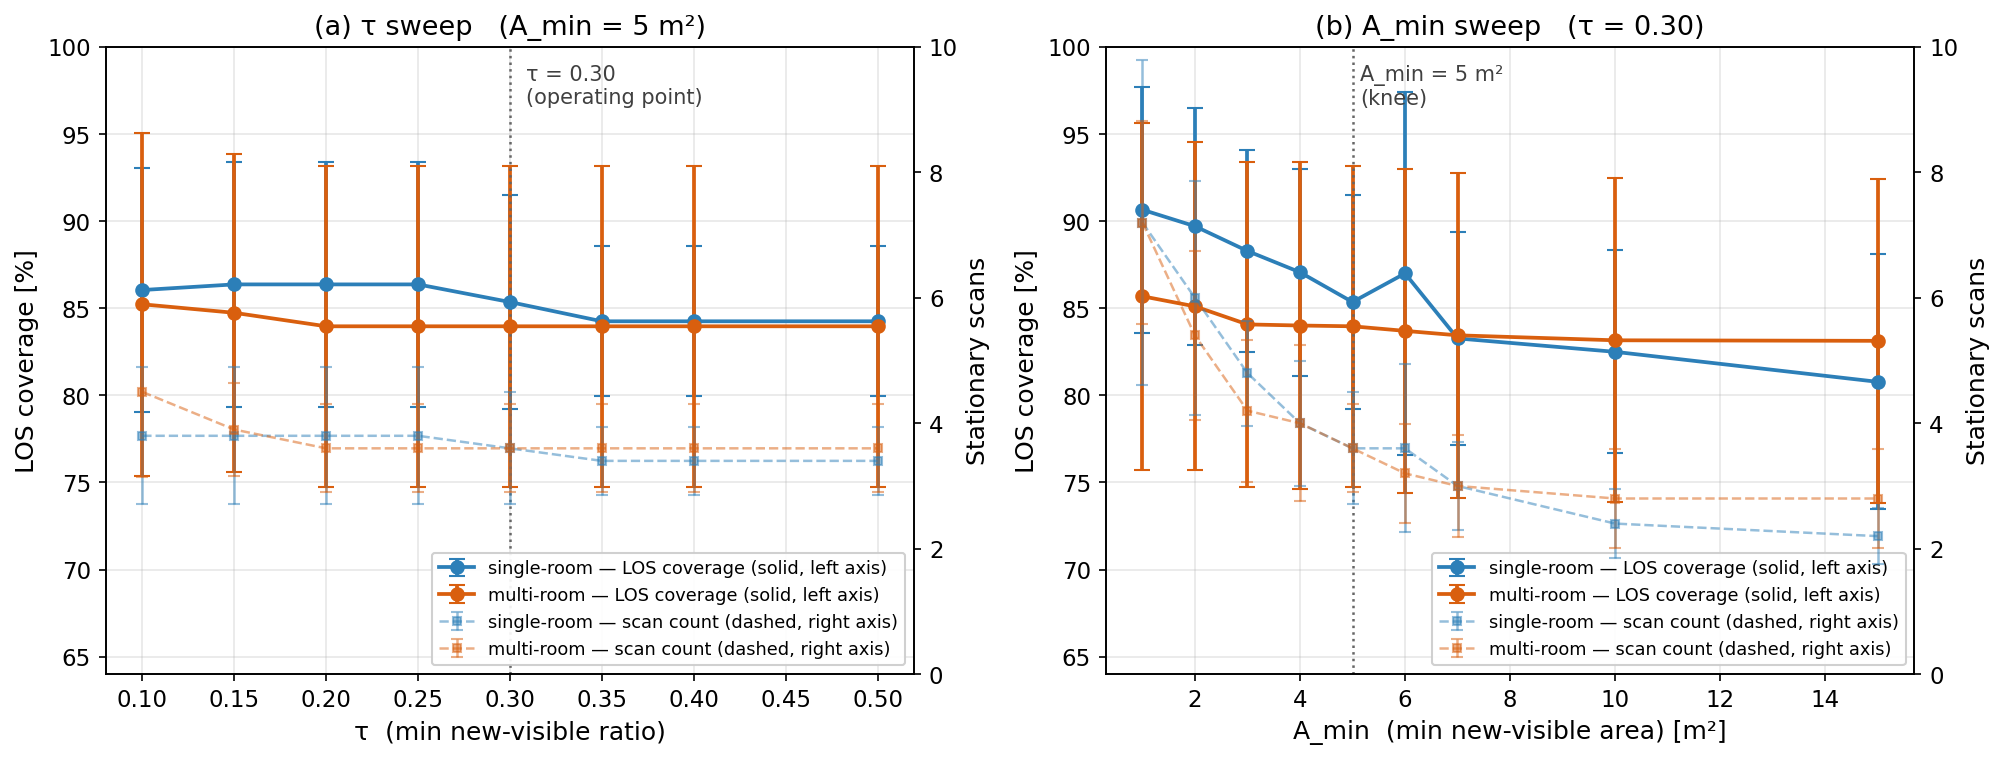
\includegraphics[width=0.95\linewidth]{figures/sen_fig8_param_sweep.png}
\caption{Parameter sweep by deterministic replay on the fixed candidate paths
(mean~$\pm$~s.d.). Solid curves: LOS coverage; dashed curves: scan count.
(a)~$\tau$ sweep at $A_{\min}=5$~m$^2$; (b)~$A_{\min}$ sweep at $\tau=0.30$,
knee marked.}
\label{fig:sweep}
\end{figure}

\subsection{Fully Autonomous On-Hardware Comparison}
\label{subsec:exp-hardware}

To test whether this behavior carries over to the physical platform, a fully
autonomous on-hardware comparison was conducted in the industrial test room:
RedBOT04 explores the room live under frontier exploration through the full
Nav2 stack while Cartographer builds the map online from the onboard 2D
LiDAR, and the stop-and-scan sequencer applies the placement policy in real
time; at each accepted pose the platform halts and the deck-mounted BLK360
acquires a full-dome stationary scan (Figure~\ref{fig:field}). Each run is
driven end to end by one skip rule---disk or visibility---so the comparison
exercises the entire pipeline on real hardware. Of the on-hardware runs, the
$N=4$ per policy that completed a room-spanning traverse are retained; two
additional early-terminated runs, in which frontier exploration stalled
shortly after start before the placement policy faced any consequential
decision, are discarded as failed trials independent of the skip rule. Every
run is evaluated on the single most complete SLAM map among the runs. Unlike
the simulated ablation, hardware runs cannot be paired, so this experiment
complements the confound-free ablation with ecological validity.

\begin{figure}[!htb]
\centering
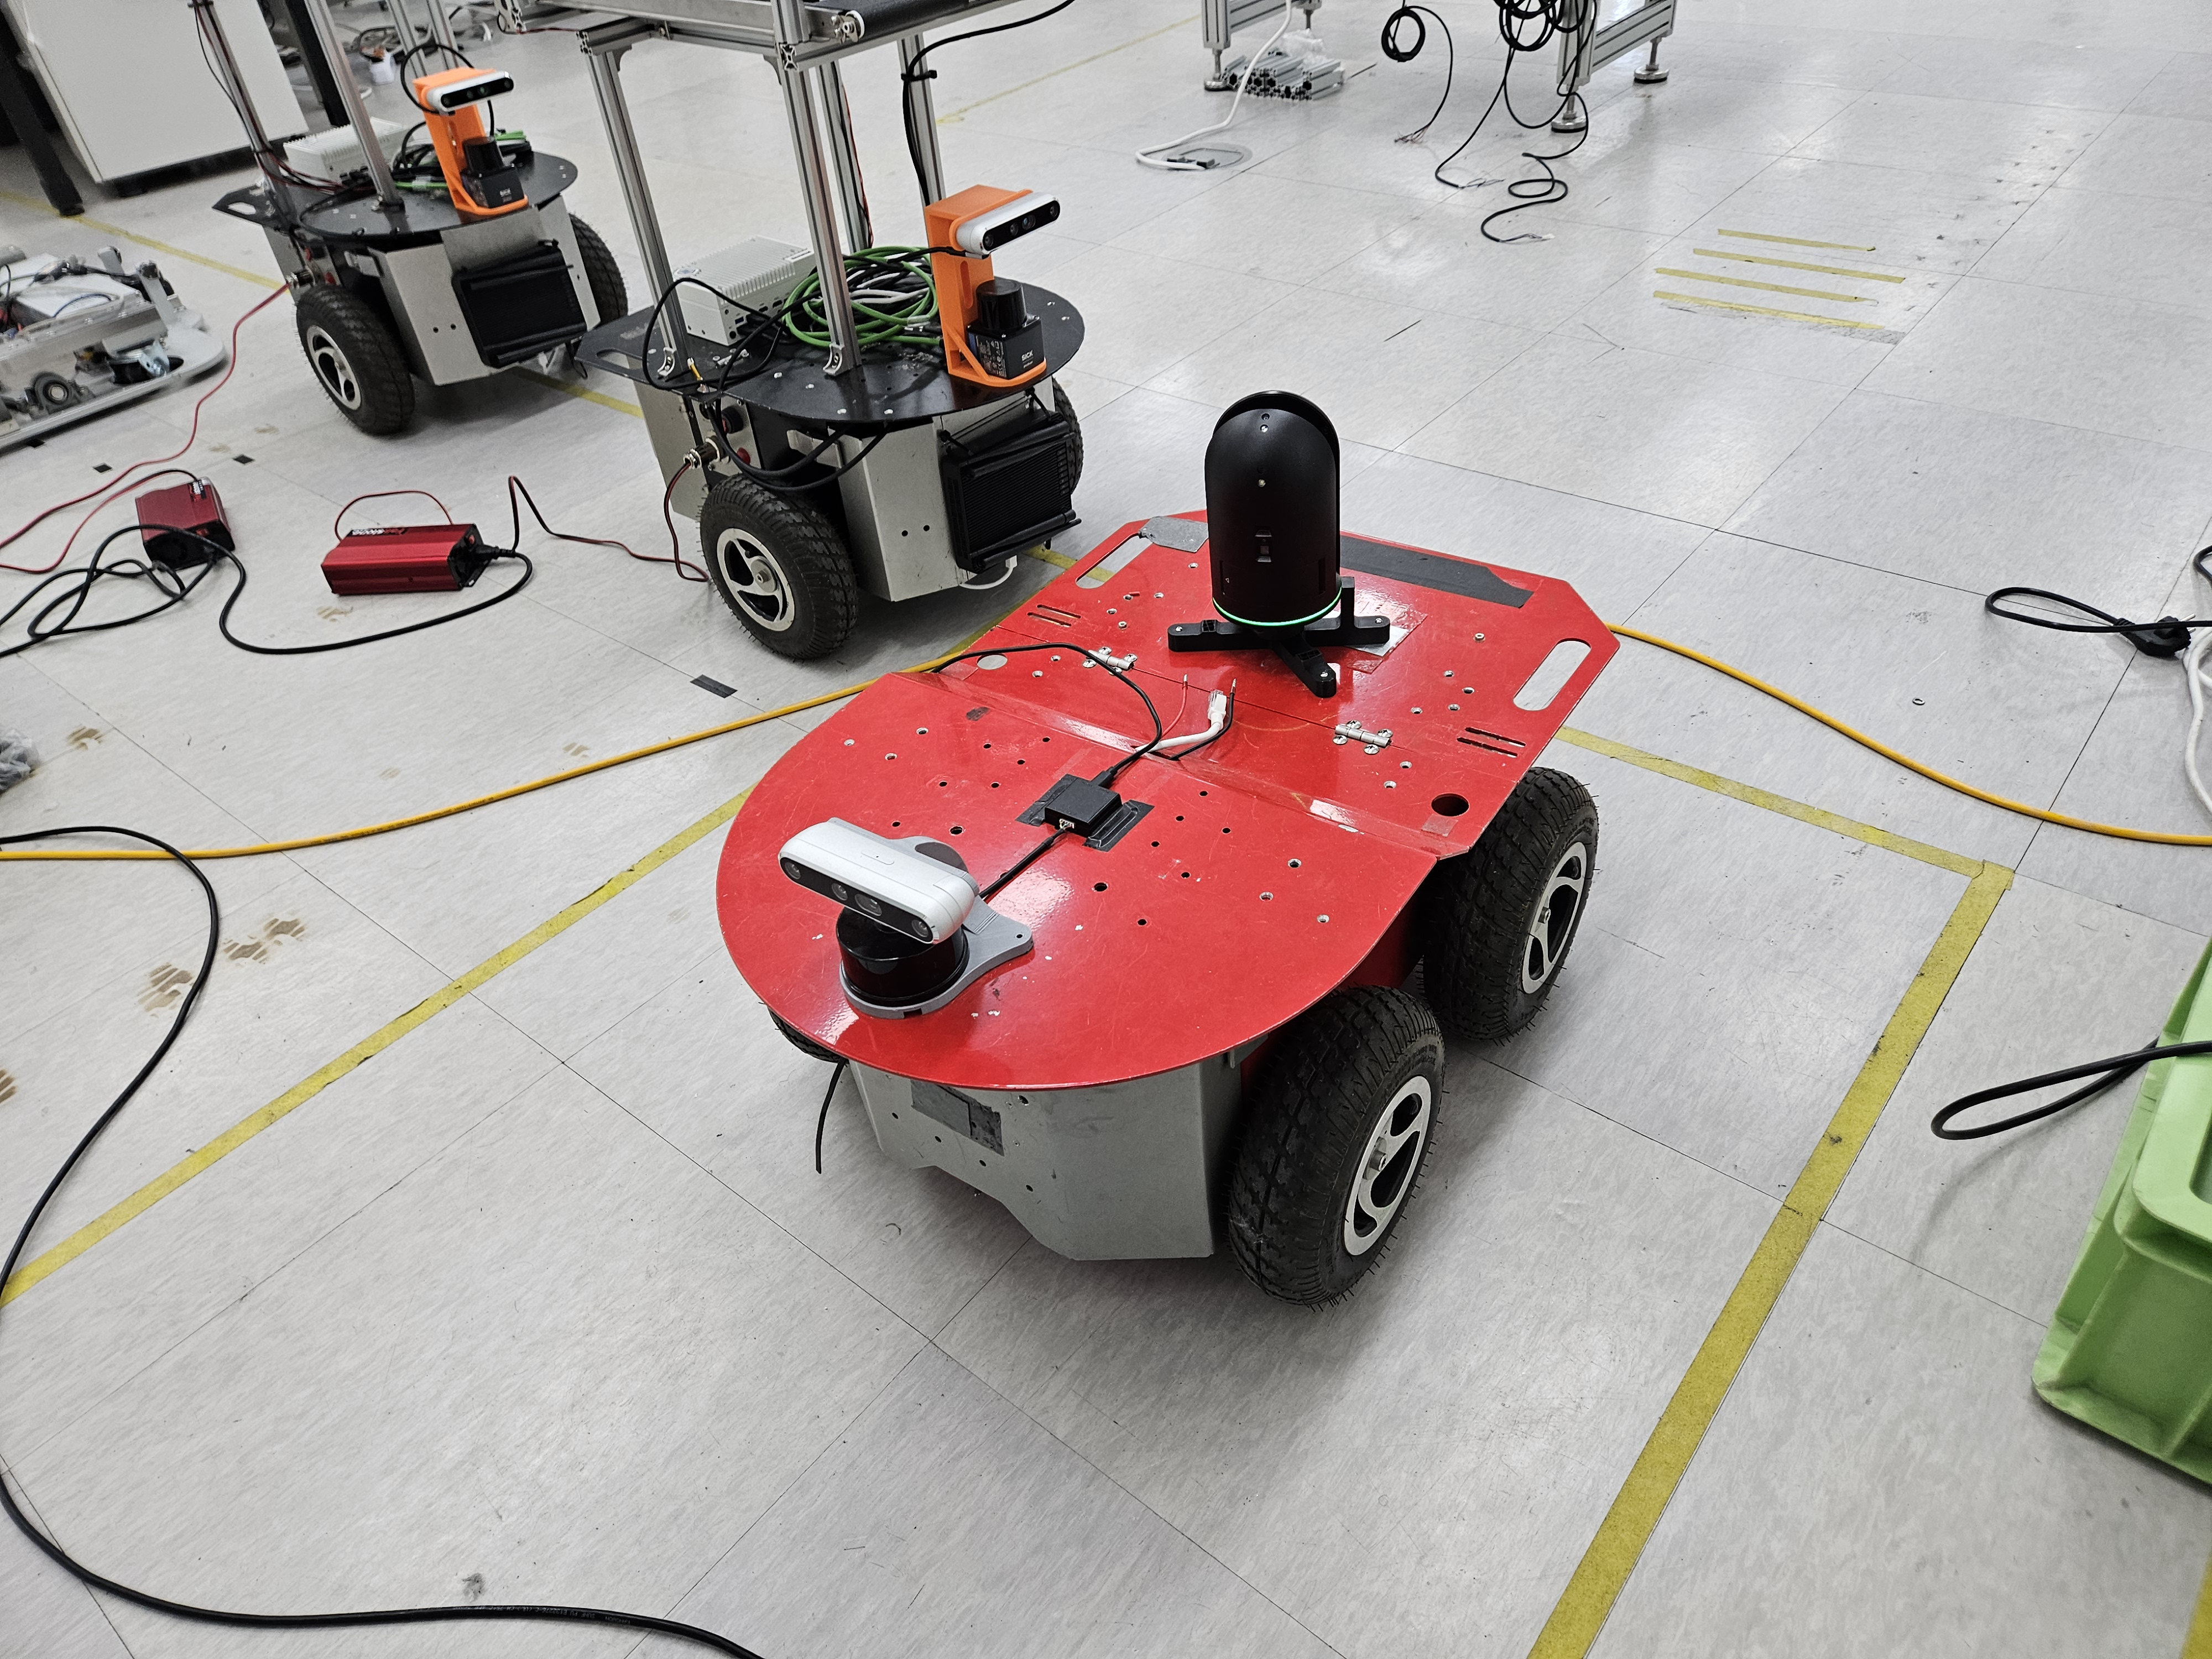
\includegraphics[width=0.82\linewidth]{figures/sen_fig13_redbot04_field.jpg}
\caption{RedBOT04 deployed in the industrial test room during the fully
autonomous on-hardware runs, with the Leica BLK360~G1 on its deck.}
\label{fig:field}
\end{figure}

The outcome reproduces the controlled ablation on the physical platform---a
platform kinematically and dimensionally different from the simulated
base---indicating that the effect is a property of the coverage model rather
than of any particular robot (Table~\ref{tab:fieldsim}, Figure~\ref{fig:fieldsim}).
The isotropic disk over-skips: it places only $1.8\pm0.5$ scans and, treating
floor behind the equipment island and furniture as covered, attains
$77.6\pm10.5\%$ LOS coverage with a large run-to-run variance, since whether
its few stations happen to see the occluded bays is largely incidental. The
visibility rule recognizes the occluded area as unseen, places $4.2\pm1.5$
scans, and covers $92.1\pm3.8\%$ of the free space reliably at the cost of
about two extra scans.

\begin{table}[htbp]
\centering
\caption{Fully autonomous on-hardware disk-versus-visibility comparison in the
physical test room ($N=4$ completed live runs per policy on RedBOT04; all
runs evaluated on the common reference map; mean~$\pm$~s.d.). Source:
\emph{Sensors}~\cite{kim2026sensors}.}
\label{tab:fieldsim}
\begin{tabular}{l c c}
\toprule
\textbf{Coverage model} & \textbf{Scans} & \textbf{LOS coverage (\%)} \\
\midrule
Isotropic disk (baseline)   & $1.8\pm0.5$ & $77.6\pm10.5$ \\
Ray-cast visibility (ours)  & $4.2\pm1.5$ & $\mathbf{92.1\pm3.8}$ \\
\bottomrule
\end{tabular}
\end{table}

\begin{figure}[!htb]
\centering
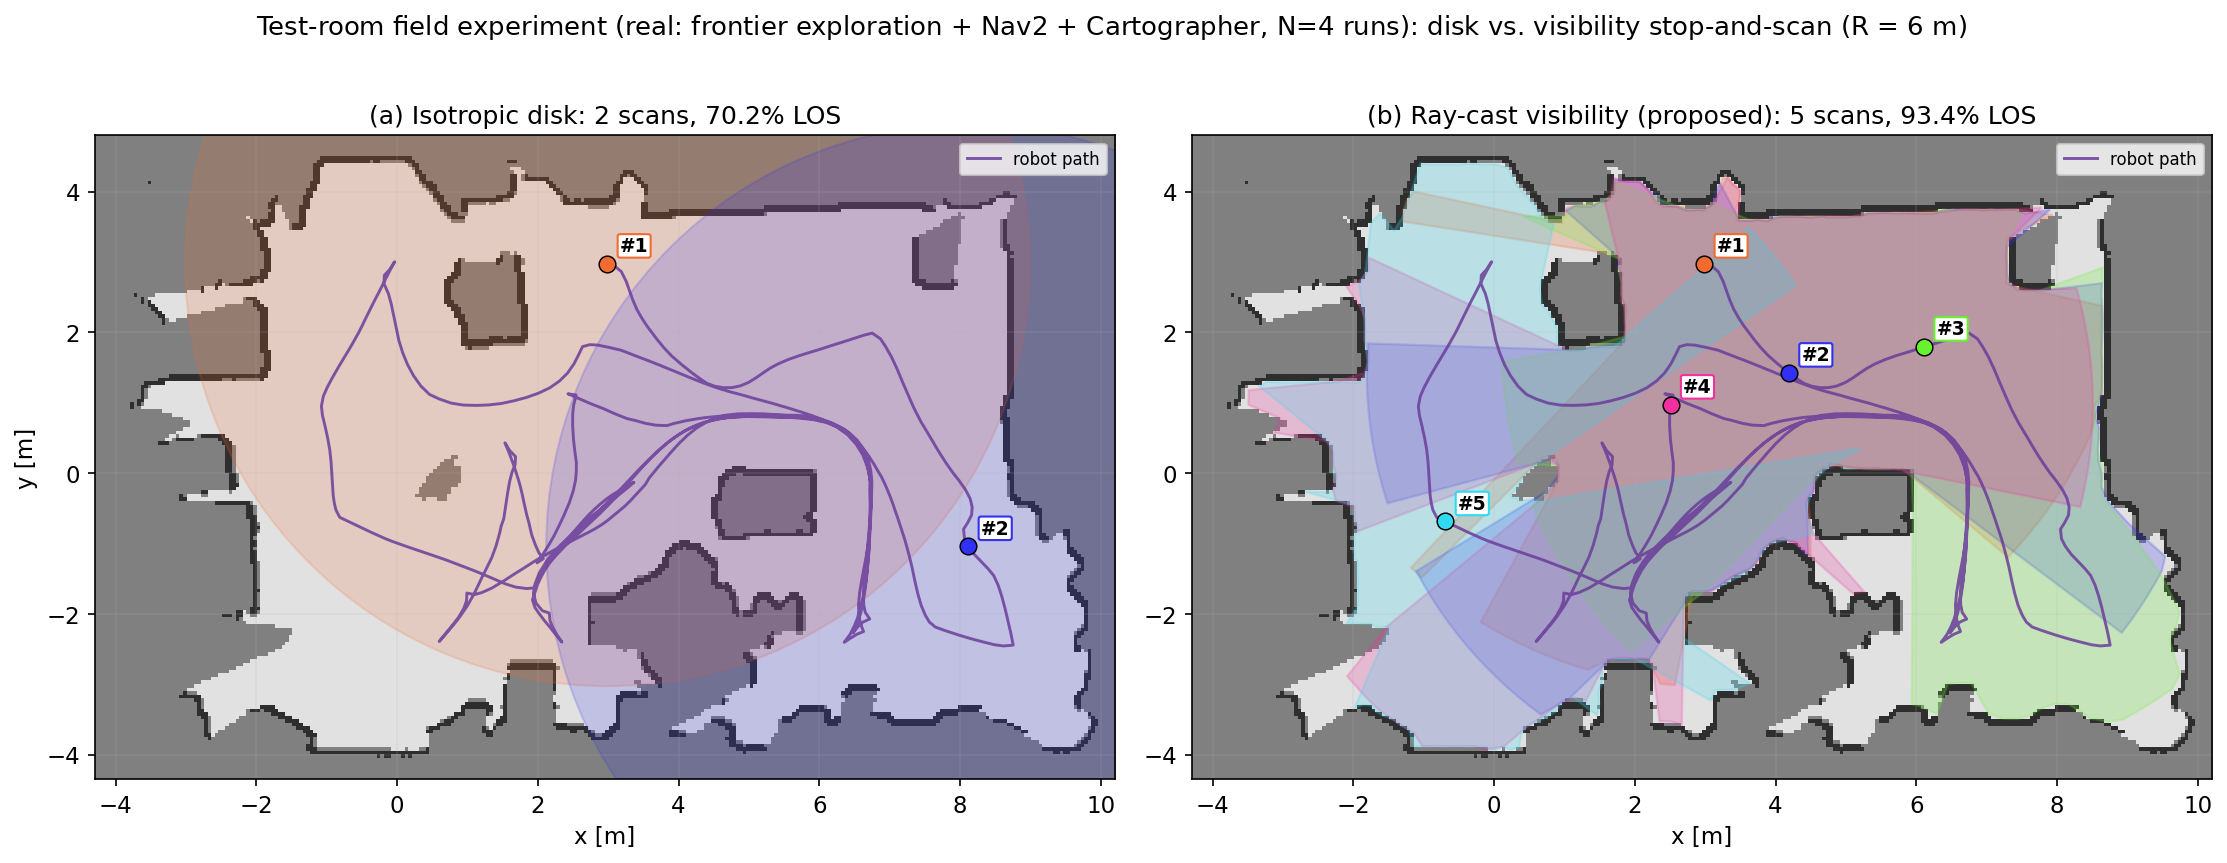
\includegraphics[width=\linewidth]{figures/sen_fig14_testroom_fieldsim.png}
\caption{Fully autonomous on-hardware comparison in the physical test room
(representative runs; $R=6$~m). Light gray: mapped free space; dark gray:
unmapped; black: occupied; purple line: autonomous robot path; colored
markers: placed scans with their coverage regions. (a)~Disk spacing rule;
(b)~visibility rule.}
\label{fig:fieldsim}
\end{figure}

\subsection{Survey-Grade Registration of the Autonomously Acquired Scans}
\label{subsec:exp-registration}

The remaining question is whether the scans each rule produces meet the
survey-grade premise. The BLK360 scans of every completed run were registered
offline, each run as an independent project under identical settings, in Leica
Cyclone REGISTER~360 PLUS using cloud-to-cloud alignment without artificial
targets (Table~\ref{tab:registration}). All four visibility runs registered at
survey grade: their networks comprise 3--6 setups joined by 3--13 pairwise
links, the bundle adjustments converged at 4--5~mm with overall overlaps of
84--88\%, and every individual link fell within the software's highest quality
band (per-link overlaps 74--92\%, errors 3--6~mm). The 4--5~mm bundle
residuals are of the same order as the scanner's stated single-setup accuracy.
The registered clouds reconstruct the room as a single coherent model
(Figures~\ref{fig:realreg} and~\ref{fig:regcloud}). The disk runs tell a
structurally different story: the three disk runs that placed two scans each
registered as a two-setup network with a single link (75--85\% overlap,
2~mm), and the fourth disk run placed only one scan and therefore admits no
registration at all. The low single-link residuals should not be read as
superior registration: with one link there is no redundancy, so the alignment
is not cross-checked by any independent constraint, and the resulting model
covers correspondingly less of the room. Bundle strengths are moderate
(38--48\%) across runs, reflecting the corridor-like traverses the explorer
takes; a loop-closing station layout, which the coverage-completion phase
naturally drives, would raise this redundancy measure.

\begin{table}[htbp]
\centering
\caption{Per-run offline registration of the autonomously acquired scans
(Leica Cyclone REGISTER~360 PLUS; cloud-to-cloud, no targets, identical
settings). Every link of every registered network lies within the software's
highest quality band (maximum error $\le15$~mm). Source:
\emph{Sensors}~\cite{kim2026sensors}.}
\label{tab:registration}
\begin{tabular}{l l c c c c}
\toprule
\textbf{Policy} & \textbf{Run} & \textbf{Setups} & \textbf{Links} & \textbf{Overall overlap (\%)} & \textbf{Bundle error (mm)} \\
\midrule
Visibility & 1 & 3 & 3  & 86 & 5 \\
Visibility & 2 & 6 & 13 & 86 & 5 \\
Visibility & 3 & 5 & 10 & 84 & 5 \\
Visibility & 4 & 3 & 3  & 88 & 4 \\
\midrule
Disk & 1 & 1 & 0 & \multicolumn{2}{c}{not registrable (single setup)} \\
Disk & 2 & 2 & 1 & 75 & 2 \\
Disk & 3 & 2 & 1 & 85 & 2 \\
Disk & 4 & 2 & 1 & 84 & 2 \\
\bottomrule
\end{tabular}
\end{table}

\begin{figure}[!htb]
\centering
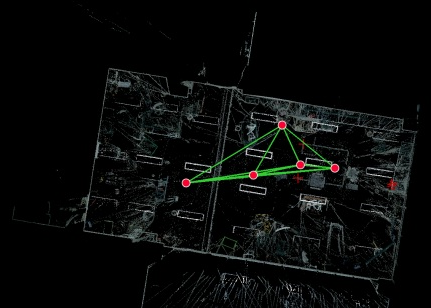
\includegraphics[height=5.0cm]{figures/sen_fig15_reg_network_vis.png}\hfill
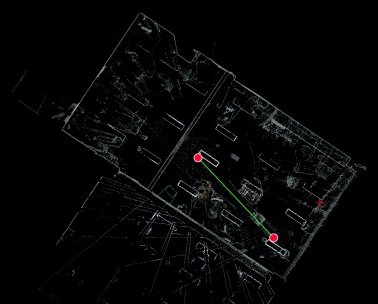
\includegraphics[height=5.0cm]{figures/sen_fig16_reg_network_disk.png}
\caption{Registered scan-station networks (top-down view; red markers are
setup positions, green edges are cloud-to-cloud links). (Left)~Visibility
run~3: five setups joined by ten redundant links reconstruct the room as a
single coherent model. (Right)~Disk run~4: two setups joined by a single
link---a minimal network with no redundant constraint.}
\label{fig:realreg}
\end{figure}

\begin{figure}[!htb]
\centering
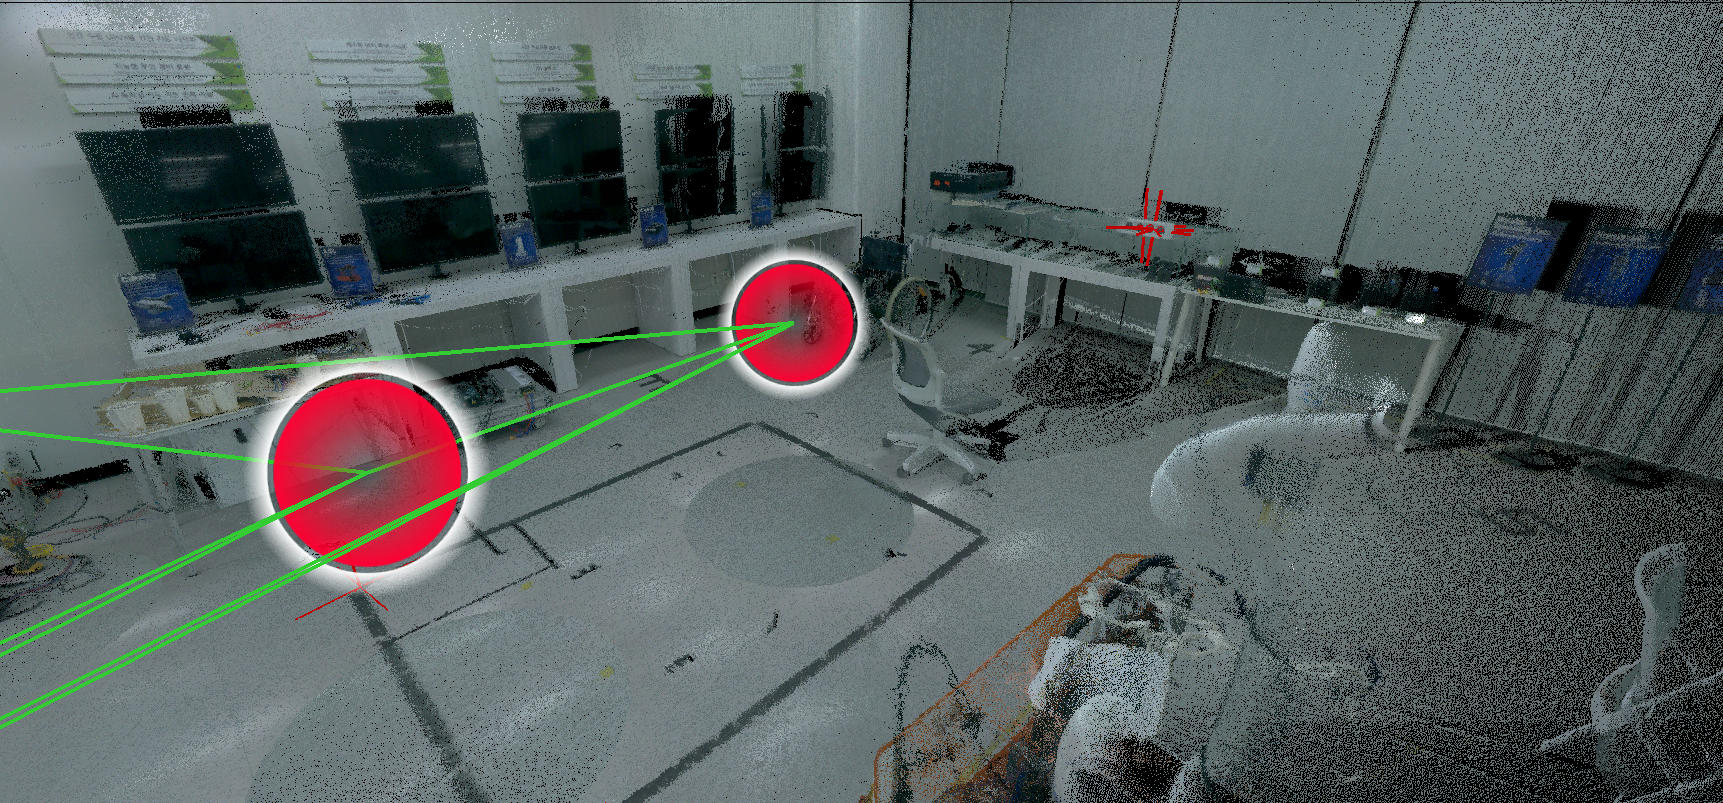
\includegraphics[width=0.49\linewidth]{figures/sen_fig17_regcloud_wall.png}\hfill
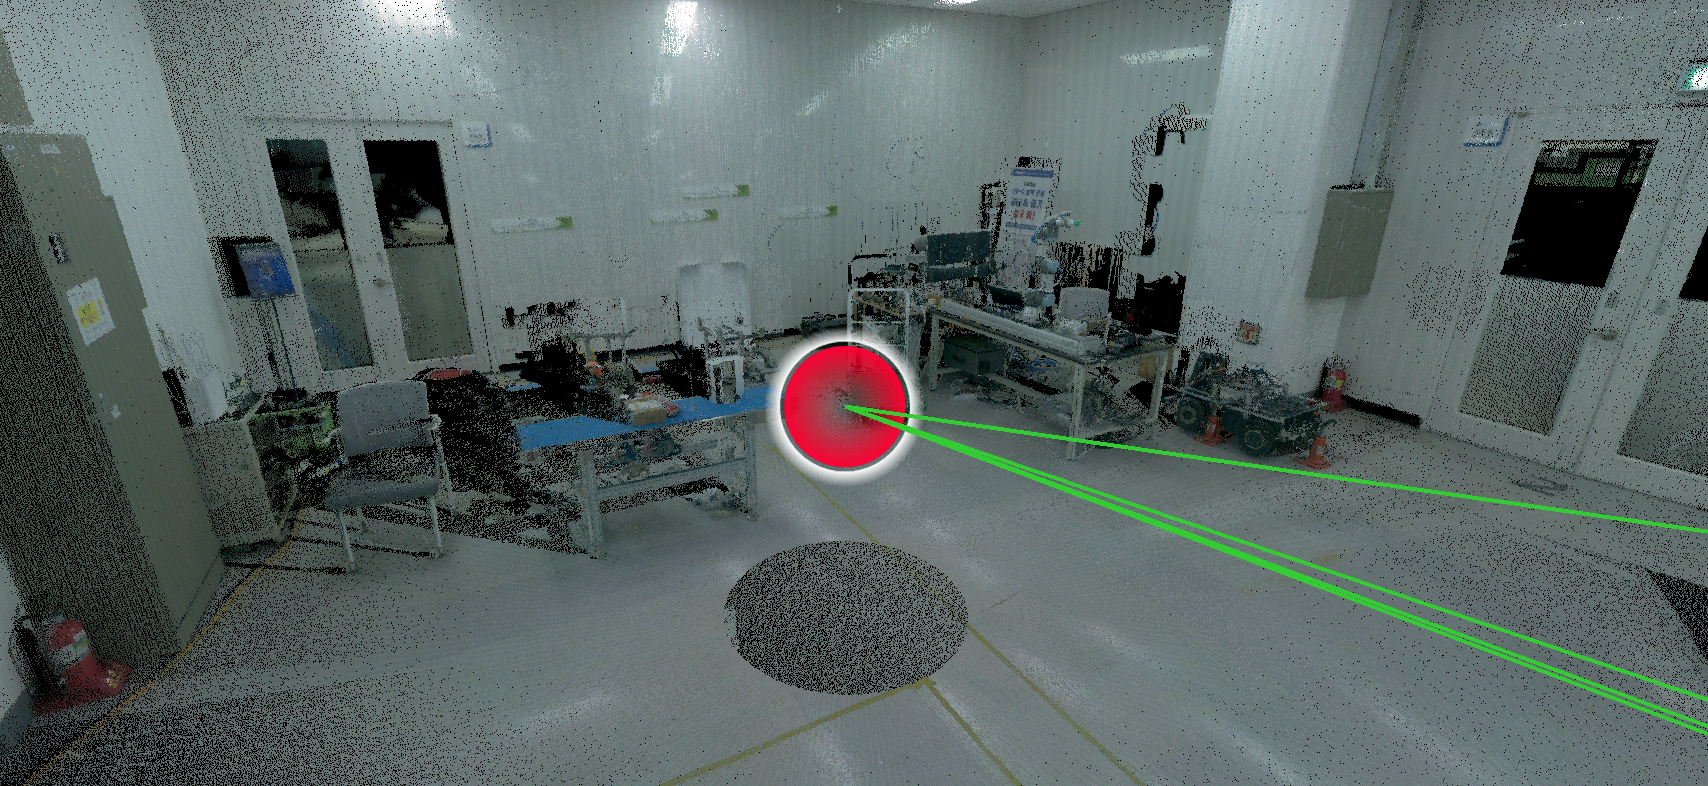
\includegraphics[width=0.49\linewidth]{figures/sen_fig18_regcloud_equipment.png}
\caption{Interior views of the registered colorized point cloud of visibility
run~3 along two diagonal directions: toward the display wall (left) and toward
the equipment side (right).}
\label{fig:regcloud}
\end{figure}

Together, the live comparison establishes that the visibility rule, not the
disk rule, reliably produces high-LOS scan placements, and the per-run
registration establishes that those placements consistently yield
survey-grade, bundle-verifiable scan networks, while disk placements do not
even guarantee a registrable network. The registered T2 and T3 clouds of
Table~\ref{tab:scenes} are the products of this subsystem that enter the
semantic modeling experiments below.

\section{Segmentation: Repeatability, Filtering, and Backbone Selection}
\label{sec:exp-seg}

\subsection{Backbone Selection against Learned Alternatives}
\label{subsec:exp-backbone}

The DBSCAN\,+\,Uni3D backbone was chosen against learned alternatives on a
wall-removed industrial scene of the test room (122.7~K points after
structural-plane removal; Figure~\ref{fig:nowallscene}). Because no point-level
ground truth exists for this scene, the metrics are deliberate screening
proxies: point \emph{coverage}, the fraction of input points assigned to some
object; the fraction of objects the open-vocabulary classifier cannot name
(\emph{unnameable}, a boundary-quality proxy because poor cuts produce more
unrecognizable fragments); and label diversity (Table~\ref{tab:backbones}).
For segmentation, the geometric clustering is compared against two
ScanNet-pretrained deep models, the superpoint-transformer instance segmenter
SPFormer~\cite{sun2023spformer} and the semantic-segmentation backbone Point
Transformer~V3~\cite{wu2024ptv3}, with every object subsequently named by the
same Uni3D classifier; for classification, Uni3D is compared against the
depth-projection classifier PointCLIP~V2~\cite{zhu2023pointclipv2}. Two further
instance segmenters, Mask3D~\cite{schult2023mask3d} and
Part2Object~\cite{shi2024part2object}, could not be evaluated because both
depend on a sparse-convolution backend incompatible with the experimental GPU.

\begin{figure}[!htb]
  \centering
  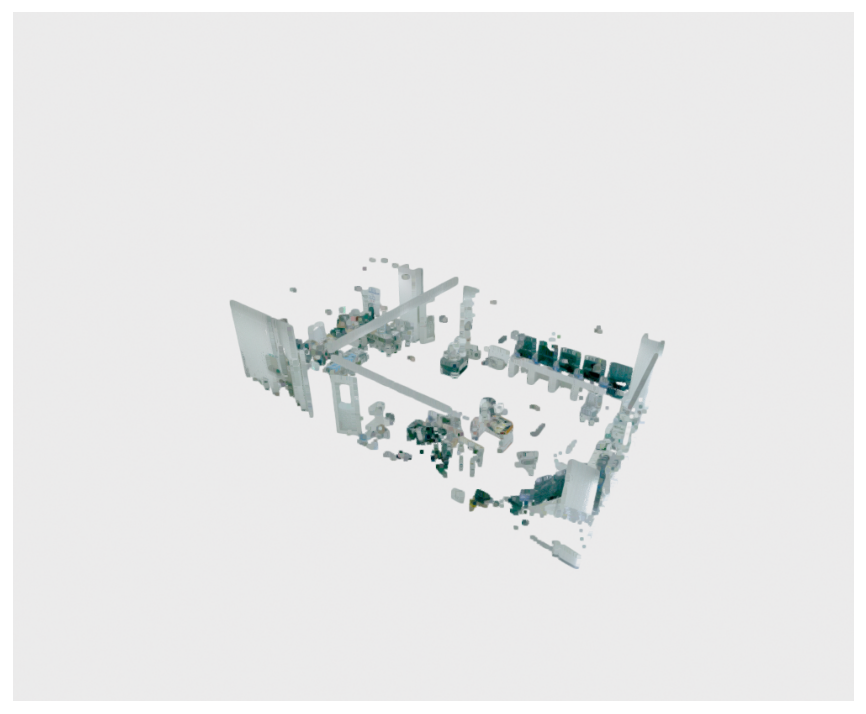
\includegraphics[width=0.7\textwidth]{figures/fig6_nowall.png}
  \caption{The backbone-selection scene: the test-room scan after
  structural-plane removal, shown in raw RGB (122{,}738 points). Only the
  object clutter remains, each connected cluster forming a candidate object.}
  \label{fig:nowallscene}
\end{figure}

\begin{table}[htbp]
\centering
\caption{Segmentation$\times$classification backbone comparison on the
wall-removed industrial scene (screening proxies; no point-level ground
truth). The PTv3 row is a semantic-segmentation head whose outputs are not
instance-comparable and is included only to document why closed-set semantic
heads were screened out.}
\label{tab:backbones}
\begin{tabularx}{\textwidth}{l c c c X}
\toprule
\textbf{Pipeline} & \textbf{Coverage} & \textbf{Unnameable} & \textbf{Classes} & \textbf{Dominant failure} \\
\midrule
\textbf{DBSCAN + Uni3D} & \textbf{98.3\%} & \textbf{23.3\%} & 13 & unlabeled coverage \\
SPFormer + Uni3D & 51.1\% & 45.9\% & 9 & furniture bias (chair 67/88) \\
PTv3 (semantic) & --- & --- & 17/20 emitted & 46\% ``wall'' after wall removal \\
DBSCAN + PointCLIP~V2 & 98.3\% & --- & 1--7 & collapse (pipe 23/30) \\
\bottomrule
\end{tabularx}
\end{table}

On every proxy, the geometric segmenter outperforms the deep closed-set model
on this out-of-distribution scene (Figure~\ref{fig:segcompare}). SPFormer
assigns only about half of the points to objects, because it fires only on
regions resembling its indoor-furniture training classes and lets genuine
industrial and robotic structure fall through; it over-segments the scene into
many partial or cross-object fragments that the classifier can no longer name,
and its label space is closed to eighteen indoor-furniture classes. PTv3 labels
46\% of all points \texttt{wall} on a scene from which the walls have already
been removed, and a further 20\% \texttt{refrigerator}: a closed-set per-point
model cannot abstain. PointCLIP~V2 collapses almost entirely to a single
category (\texttt{pipe} for 23 of 30 objects) at a deceptively high mean
confidence, because on the sparse, partial objects of a survey scan the depth
projections are too degenerate to be discriminative. The geometric backbone
wins not by being smarter but by refusing to guess: its failure mode is
unlabeled coverage, which the verification and owner layers are built to
absorb. Instance quality of the retained backbone is validated independently
below (owner-referenced sweep) and in Section~\ref{sec:exp-endtoend}
(end-to-end recall).

\begin{figure}[!htb]
  \centering
  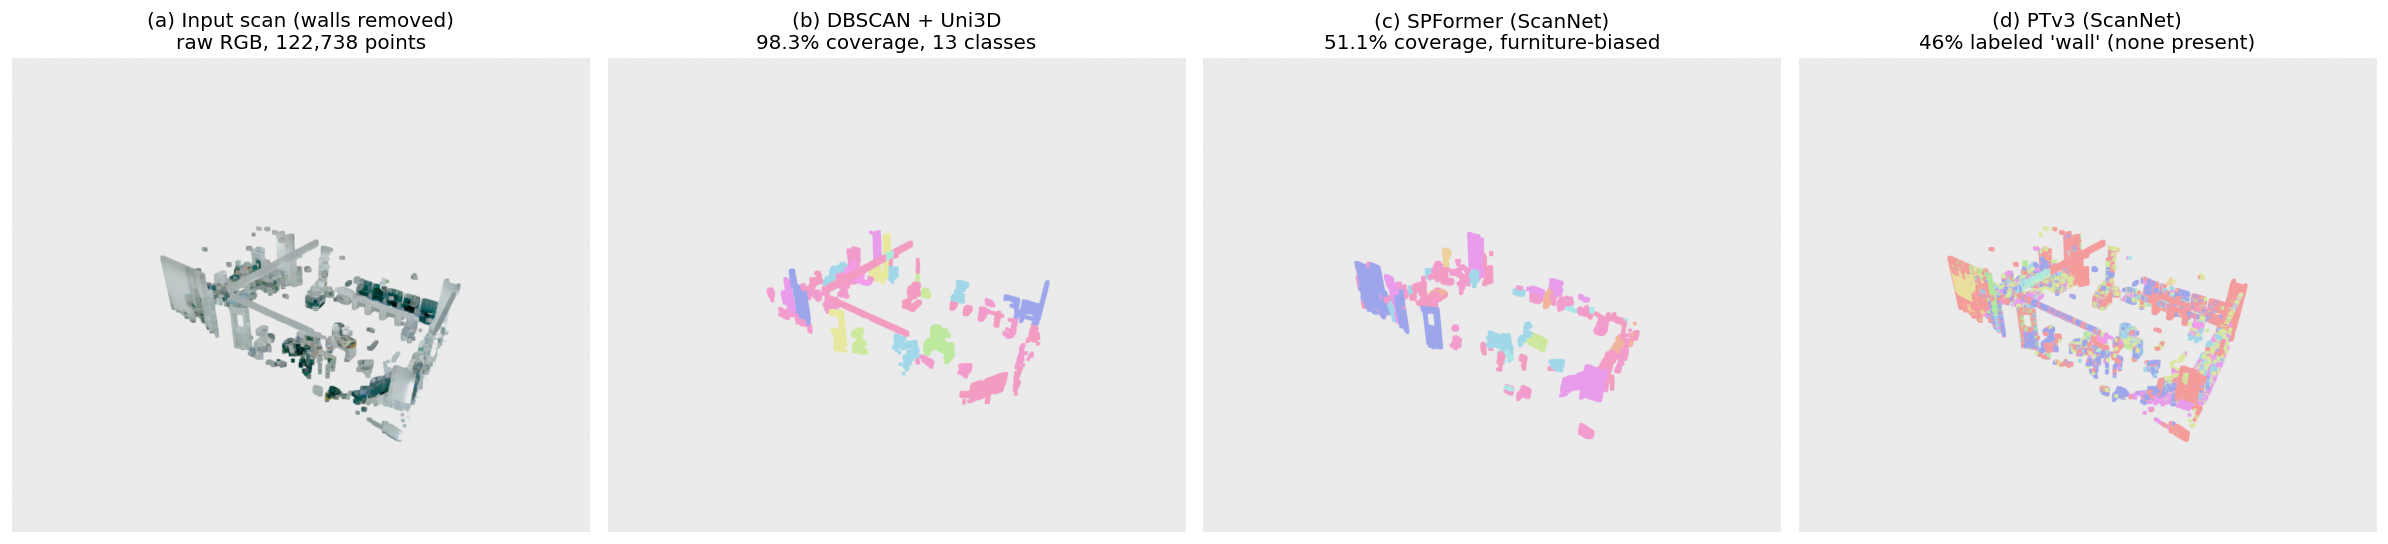
\includegraphics[width=\textwidth]{figures/fig6_2.png}
  \caption{Object segmentation on the test-room scan. (a)~The input cloud after
  wall removal (raw RGB). (b)--(d) are colored by predicted class: (b)~the
  geometric DBSCAN clustering with Uni3D labels covers the scene with coherent
  objects across 13 classes; (c)~SPFormer (ScanNet closed-set) assigns only
  about half of the points and biases toward indoor-furniture classes;
  (d)~PTv3 (ScanNet semantic) labels nearly half of the points \texttt{wall}
  although the walls were removed.}
  \label{fig:segcompare}
\end{figure}

\subsection{Repeatability and Remnant Filtering}
\label{subsec:exp-repeat}

Running the full pipeline twice from the same E57---including ten-plane
structure removal---reproduces every cluster byte-identically on both main
scenes (hash-verified). To probe robustness beyond one software stack, the
backbone was packaged into a version-pinned container and re-run under a
deliberately different environment (different glibc and Python patch
versions): all 81 retained robot-hall clusters remain byte-identical to the
native run. Running the same container on a second machine with a different
CPU vendor and microarchitecture (an Intel Core i9-13900H laptop versus the AMD
reference workstation) reproduces the identical per-cluster checksums---the
determinism claim holds across operating environments and x86-64 CPU vendors
under the pinned library set; bit-level reproducibility across instruction-set
architectures is not claimed. The structure-remnant filter of
Section~\ref{subsec:decomposition} removed all fourteen owner-confirmed
ceiling-soffit phantoms (seven per scene: showroom $45\rightarrow38$, robot
hall $88\rightarrow81$) while leaving every retained cluster unchanged. Before
the filter, these phantoms produced confidently verified fictions (keyboard
panels, handrails) that survived multi-view voting, since every view showed the
same wall-colored slab; detecting structure remnants geometrically, upstream of
semantics, proved more reliable than asking the verifier to doubt itself.

\subsection{Parameter Sensitivity and Coverage Stress}
\label{subsec:exp-params}

A 36-combination sweep (giant-split footprint $\times$ DBSCAN $\varepsilon$
$\times$ minimum points) shows a stable plateau at footprint 2.0--2.5~m:
instance recall degrades at 3.0~m as neighbors merge and at 1.5~m as equipment
shatters. Because scoring a sweep against the operating point's own
decomposition would be circular, every combination was re-scored against an
independent object-level reference: the owner-audited inventory in a
membership-independent form (all clean-cloud points falling inside each
owner-audited oriented box). On the robot hall (42 reference objects) the
min-points-100 band is a broad plateau and the operating point (2.5~m / 0.30 /
100) sits at the grid maximum (recall 0.952). On the showroom, the audit
surfaced an error, which is reported plainly: against the genuinely audited 57-object
inventory no grid combination of the base clustering exceeds recall 0.33---the
audited granularity of that scene is produced by the split-refinement stage,
not by any base-DBSCAN setting---so the parameter-robustness claim rests on the
non-circular robot-hall table. Two further perturbations bound the geometric
operating regime: voxel size is part of a jointly calibrated triple with
$(\varepsilon,\mathrm{min\_points})$ (at 3~cm the backbone recovers 42/42
reference objects, but 2~cm collapses recall to 0.36 as 22 objects merge and
5~cm to 0.33 as small objects starve), and seeded per-point Gaussian noise at
$\sigma=5$~mm---the scale of the scanner's real bundle error---drops recall to
0.48, with the 5~cm RANSAC inlier band saturating first. The T3 epoch supplied
a coverage stress case: at 99.6\% coverage, inter-object gaps close and DBSCAN
chains 120~K points (41\% of the clean cloud) into one $10.4\times9.6$~m
mega-cluster that survives the giant-split; refinement recovers little of the
resulting diff inflation, which is itself informative: about 88\% of that
epoch's absences reflect genuine scene change, not segmentation artifacts.

\subsection{Corrective Layers in Operation}
\label{subsec:exp-corrective}

Two T3 clusters that survived every upstream filter are \emph{diffuse webs}:
95~K and 13~K points spread over 80 and 12~m$^2$ at a 2D occupancy fill below
0.3, connected at $\sim$1.8~cm point spacing at any usable $\varepsilon$. The
diffuseness-gated re-split resolves them by \emph{cause} instead of size:
points hugging the exploration-grid wall line are structure noise ($\sim$70\%
of the 95~K-point residual), out-of-room bleed-through accounts for another 7\%,
and the remainder is re-clustered by occupancy-core erosion and split at the
support plane. The owner's ground truth for the largest compound---``a robot
arm on a desk, part of a mobile robot, wall noise''---is recovered exactly.
Applied to a 6.2~m wall-flush cluster that verification had confidently labeled
\texttt{electrical cabinet} (0.83), the wall-compound gate recovers the owner's
inventory at unit granularity: nine of the ten owner-confirmed monitor units,
the desk beneath them, and, from the off-wall remainder, a wheelchair robot;
unit boundaries are approximate because the dark screens return few points,
so the result is claimed as unit-level recall, not precise per-unit
segmentation. The structure-condition ensemble recovered two multi-meter
tables that exist in \emph{no} single-condition segmentation of the production
path---they appear only when walls are left in place---raising in-room recall
by four real objects ($\sim$8\%) as a standalone pass. The fusion also
quantifies label fragility: only 10 of 37 re-found objects keep the same label
across conditions, and cross-condition \emph{voting} corrected nothing, because
the verifier's biases are correlated across conditions (both recovered tables
were unanimously mis-verified as conveyor belts in every condition). Under a
pre-specified adoption rule, Point-SAM~\cite{zhou2024pointsam} separated 3/6
flagged merged clusters with sub-cluster labels reaching 9/11 versus 5/11 for
their parents, but automatic candidate selection also produced 2/6 false
positives, so it is retained only as an optional, manually triggered diagnostic
refinement (Figure~\ref{fig:baselines}).

\begin{figure}[!htb]
\centering
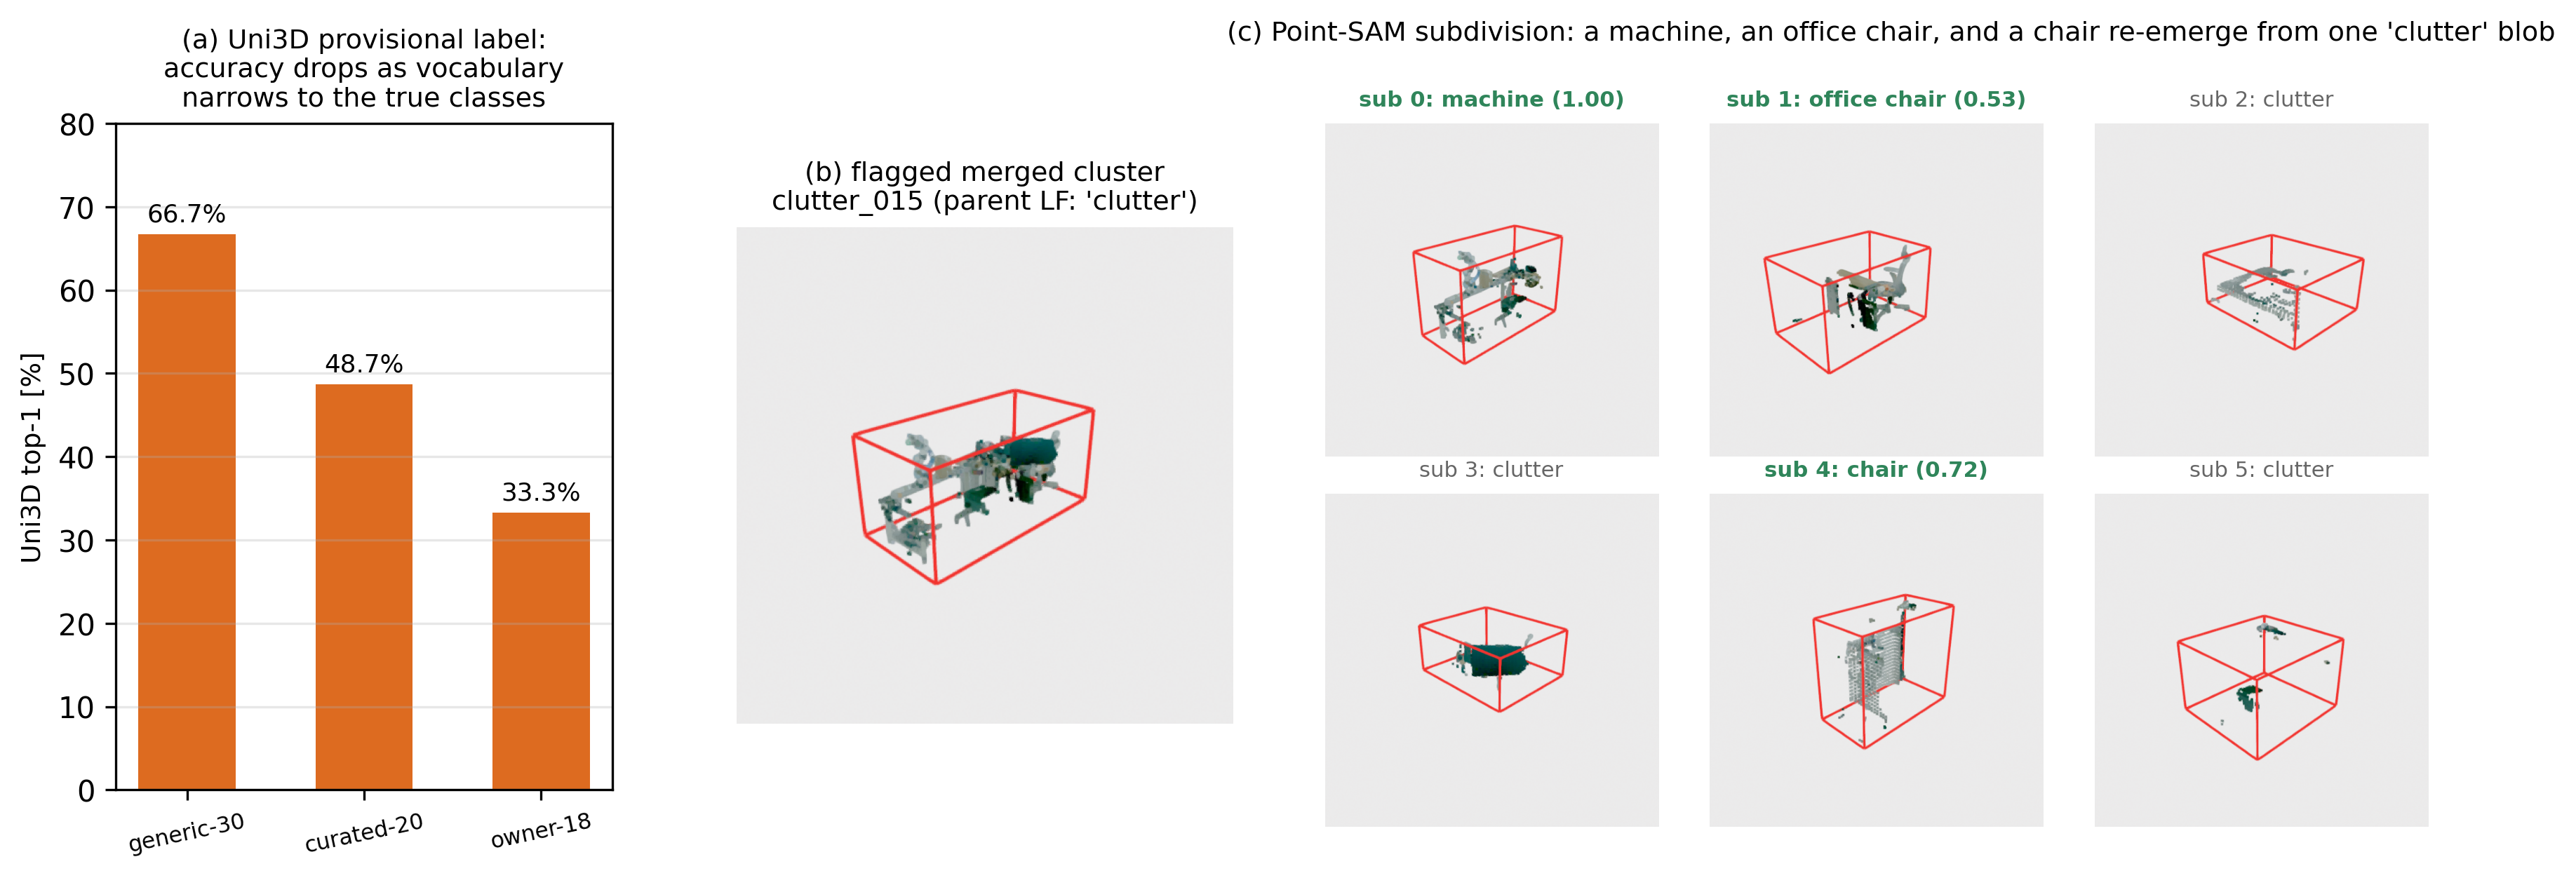
\includegraphics[width=0.95\linewidth]{figures/ele_fig13_pointsam_uni3d.png}
\caption{Learned components used as bounded tools. (a)~The Uni3D provisional
label degrades as the vocabulary narrows to the deployment's true classes
(Section~\ref{sec:exp-ablation})---why it is treated as untrusted context.
(b,c)~Conditional Point-SAM refinement of a flagged merged cluster: a machine,
an office chair, and a chair re-emerge from a single \texttt{clutter} blob,
each re-verified independently.}
\label{fig:baselines}
\end{figure}

\section{Verification: Multi-View Fusion and Escalation}
\label{sec:exp-verify}

\subsection{Multi-View Fusion Study}
\label{subsec:exp-multiview}

The first verification study, on the 57-object showroom decomposition, asks
how a VLM should consume multiple rendered views. Six configurations are
compared: a classifier-only reference, a $2\times2$ design over view count
(1 vs.\ 4, early fusion) and render/prompt generation (sparse renders with a
base prompt vs.\ dense renders with the guardrail prompt), and a sixth that
differs from four-view early fusion only in the fusion rule
(Table~\ref{tab:configs}). Labels are graded by two
independent references: a render audit by two of the authors against the dense
four-view renders and the measured dimensions, and the on-site inventory of the
facility operator by physical inspection, without reference to the render
audit. Audit-versus-inventory agreement is 79--95\% over the five VLM
configurations (Cohen's $\kappa$ 0.53--0.89). Three findings stand out
(Figure~\ref{fig:accuracy}).

\begin{table}[htbp]
\caption{Final type labels (57 showroom objects) under both references. Render
audit: C/P/W = correct / plausible / wrong, strict = C, lenient = C+P.
Inventory: strict matches on all 57 objects and on the 36 confirmed
non-structure objects. Source: ICTC~2026~\cite{kim2026ictc}.}
\label{tab:configs}
\centering
\begin{tabular}{l c c c c c c c}
\toprule
 & \multicolumn{5}{c}{\textbf{Render audit}} & \multicolumn{2}{c}{\textbf{Inventory}} \\
\textbf{Configuration} & C & P & W & strict & lenient & 57 & 36 \\
\midrule
Uni3D only (no VLM)            & 28 & 5  & 24 & 49\% & 58\% & 33 & 28 \\
1 view, base prompt, sparse    & 34 & 12 & 11 & 60\% & 81\% & \textbf{44} & \textbf{33} \\
4 views early fusion, sparse   & 28 & 10 & 19 & 49\% & 67\% & 34 & 27 \\
1 view, guardrails, dense      & 29 & 11 & 17 & 51\% & 70\% & 32 & 29 \\
4 views early fusion, dense    & 26 & 12 & 19 & 46\% & 67\% & 30 & 23 \\
4 views late fusion, dense     & 28 & \textbf{14} & \textbf{15} & 49\% & \textbf{74\%} & 34 & 28 \\
\bottomrule
\end{tabular}
\end{table}

\begin{figure}[!htb]
\centering
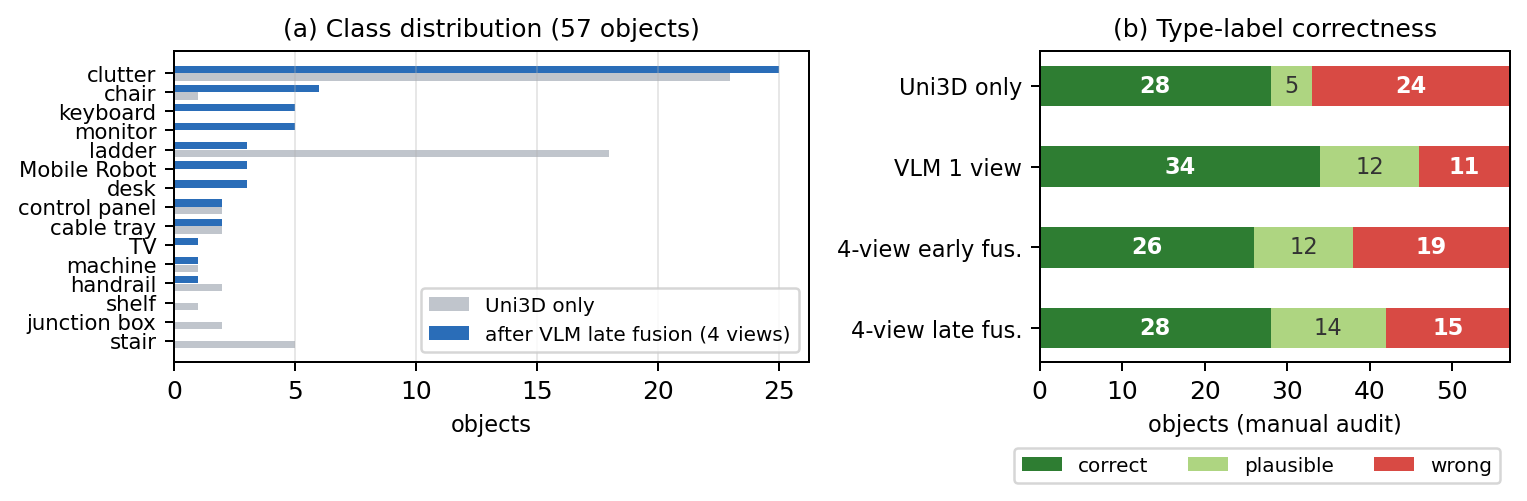
\includegraphics[width=0.95\linewidth]{figures/ictc_fig_accuracy.png}
\caption{Effect of VLM verification on the 57-object showroom scene.
(a)~Class distribution, classifier-only vs.\ after late fusion: implausible
\emph{ladder}/\emph{stair} populations are redistributed to displays and
furniture. (b)~Render audit: early fusion degrades single-view accuracy; late
fusion is the strongest multi-view strategy (15 wrong labels vs.\ 19 for
early fusion).}
\label{fig:accuracy}
\end{figure}

\emph{Early fusion hurts.} Feeding four sparse views into one prompt dropped
strict accuracy from 60\% (single view) to 49\%: extra oblique speckle views
encouraged over-committed readings, e.g., two electrical cabinets confidently
relabeled \emph{chair}; denser renders and the guardrails did not close the
gap, and the inventory confirms the direction. \emph{Late fusion is the
strongest multi-view strategy, but not the best configuration.} Judging each
view independently and voting beats early fusion on every measure (15 vs.\ 19
wrong labels, 74\% vs.\ 67\% lenient; 34 vs.\ 30 inventory matches) because a
contaminated view is outvoted, but it does not overtake the best single
canonical view (44/57 inventory matches, 77\%, versus 34/57): on sparse point
clouds extra views add noise faster than evidence, and the vote spends much of
its gain on caution. Late fusion is therefore claimed as the safer multi-view
rule, not as an accuracy gain over a well-chosen single view. \emph{Vote
unanimity is a free precision signal.} 17 of 57 objects received identical
labels from all four views; 16 of those (94\%) were audited correct and match
the inventory, versus 30\% (audit) or 18/40 (inventory) among split-vote
objects. Two re-runs of the late-fusion protocol bound the verifier's sampling
variance: accuracy on the 36 confirmed objects was 28, 27, and 27 across three
runs, and unanimity precision 16/17, 20/21, and 19/20 (94--95\%). Render
density produced the study's starkest warning: dense renders made four
dotted-grid panels look so convincingly like keyboards (per-view confidence up
to 0.97) that the label passed the render-based audit---only the inventory
revealed them to be ceiling-soffit remnants. A label that fools both the VLM
and a human at the same renders was still caught by vote splits, the strongest
argument for gating, and the incident motivated the structure-remnant filter.
On the late-fusion output, the implicit prompt marked 6 of 57 objects as key
objects (control panels, a large machine, mobile robots, and a wall display)
and 50 as movable; Figure~\ref{fig:ictccards} shows two completed records.

\begin{figure}[!htb]
\centering
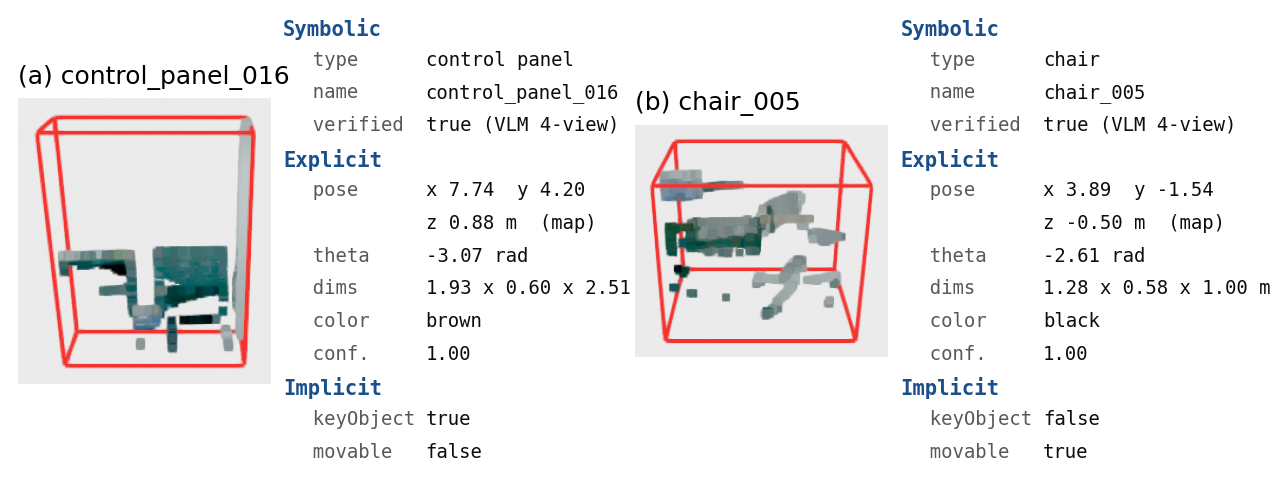
\includegraphics[width=0.95\linewidth]{figures/ictc_fig_cards.png}
\caption{Completed TOSM semantic-object records (dense render with symbolic /
explicit / implicit fields) as serialized into the VDA~5050-style message.
(a)~A control panel, unanimously verified and marked as a fixed key landmark.
(b)~An office chair corrected from \emph{stair}, movable and not a landmark.}
\label{fig:ictccards}
\end{figure}

\subsection{Escalation, Tiers, and Threshold Sensitivity}
\label{subsec:exp-escalation}

The escalation mechanism of Section~\ref{subsec:escalation} is evaluated on
both main scenes (Table~\ref{tab:verification}). Escalation lifts
confirmed-ground-truth accuracy from 77.8\% to 88.9\% on the showroom and from
78.1\% to 84.4\% on the robot hall (lenient: $76.2\%\rightarrow83.3\%$,
$n=42$), recovering 5 and 3 split-vote objects while regressing 1 and 0---a
consistent observed improvement across both scenes, though at these
sample sizes the paired contrast does not reach conventional significance
(exact McNemar $p=0.219$ and $p=0.25$), which the Wilson intervals make
explicit. Escalation adds 232 and 208 calls per scene at $\sim$\$0.009 per
call (Figure~\ref{fig:esccost}). The tier structure justifies the gating:
unanimous and escalated tiers reach 88.9--100\% precision, while the
unverified residue is 40--60\%---exactly the content the query interface must
demote. A repeat of the showroom run under identical settings bounds the
verifier's run-to-run variance at about $\pm3$ points. Verification yield
tracks scan quality: the manual scan leaves 47\% of objects unverified versus
24\% for exploration scans, and re-processing the T3 scan from a single setup
(1/6 coverage) drops the verified tier from 75.6\% to 56.6\% on identical
geometry---coverage buys verifiability, which ties Part~B back to Part~A.

\begin{table}[htbp]
\centering
\caption{Verification accuracy against confirmed ground truth, and per-tier
precision. Accuracy rows are over confirmed GT ($n=36$/32); trigger rates and
tier counts are over all GT-scored clusters (50 showroom / 51 robot hall).
Source: \emph{Electronics}~\cite{kim2026electronics}.}
\label{tab:verification}
\begin{tabular}{l c c c c}
\toprule
 & \multicolumn{2}{c}{\textbf{Showroom ($n=36$)}} & \multicolumn{2}{c}{\textbf{Robot hall ($n=32$)}} \\
 & base-4 & escalated & base-4 & escalated \\
\midrule
Accuracy & 77.8\% & \textbf{88.9\%} & 78.1\% & \textbf{84.4\%} \\
95\% Wilson CI & 61.9--88.3 & 74.7--95.6 & 61.2--89.0 & 68.2--93.1 \\
Recovered / regressed & \multicolumn{2}{c}{5 / 1} & \multicolumn{2}{c}{3 / 0} \\
Escalation trigger & \multicolumn{2}{c}{58\% (29/50)} & \multicolumn{2}{c}{51\% (26/51)} \\
\midrule
Unanimous precision & \multicolumn{2}{c}{100\% (19/19; 21 unan.)} & \multicolumn{2}{c}{94.4\% (17/18; 25 unan.)} \\
Escalated precision & \multicolumn{2}{c}{100\%} & \multicolumn{2}{c}{88.9\%} \\
Unverified precision & \multicolumn{2}{c}{60\%} & \multicolumn{2}{c}{40\%} \\
\bottomrule
\end{tabular}
\end{table}

\begin{figure}[!htb]
\centering
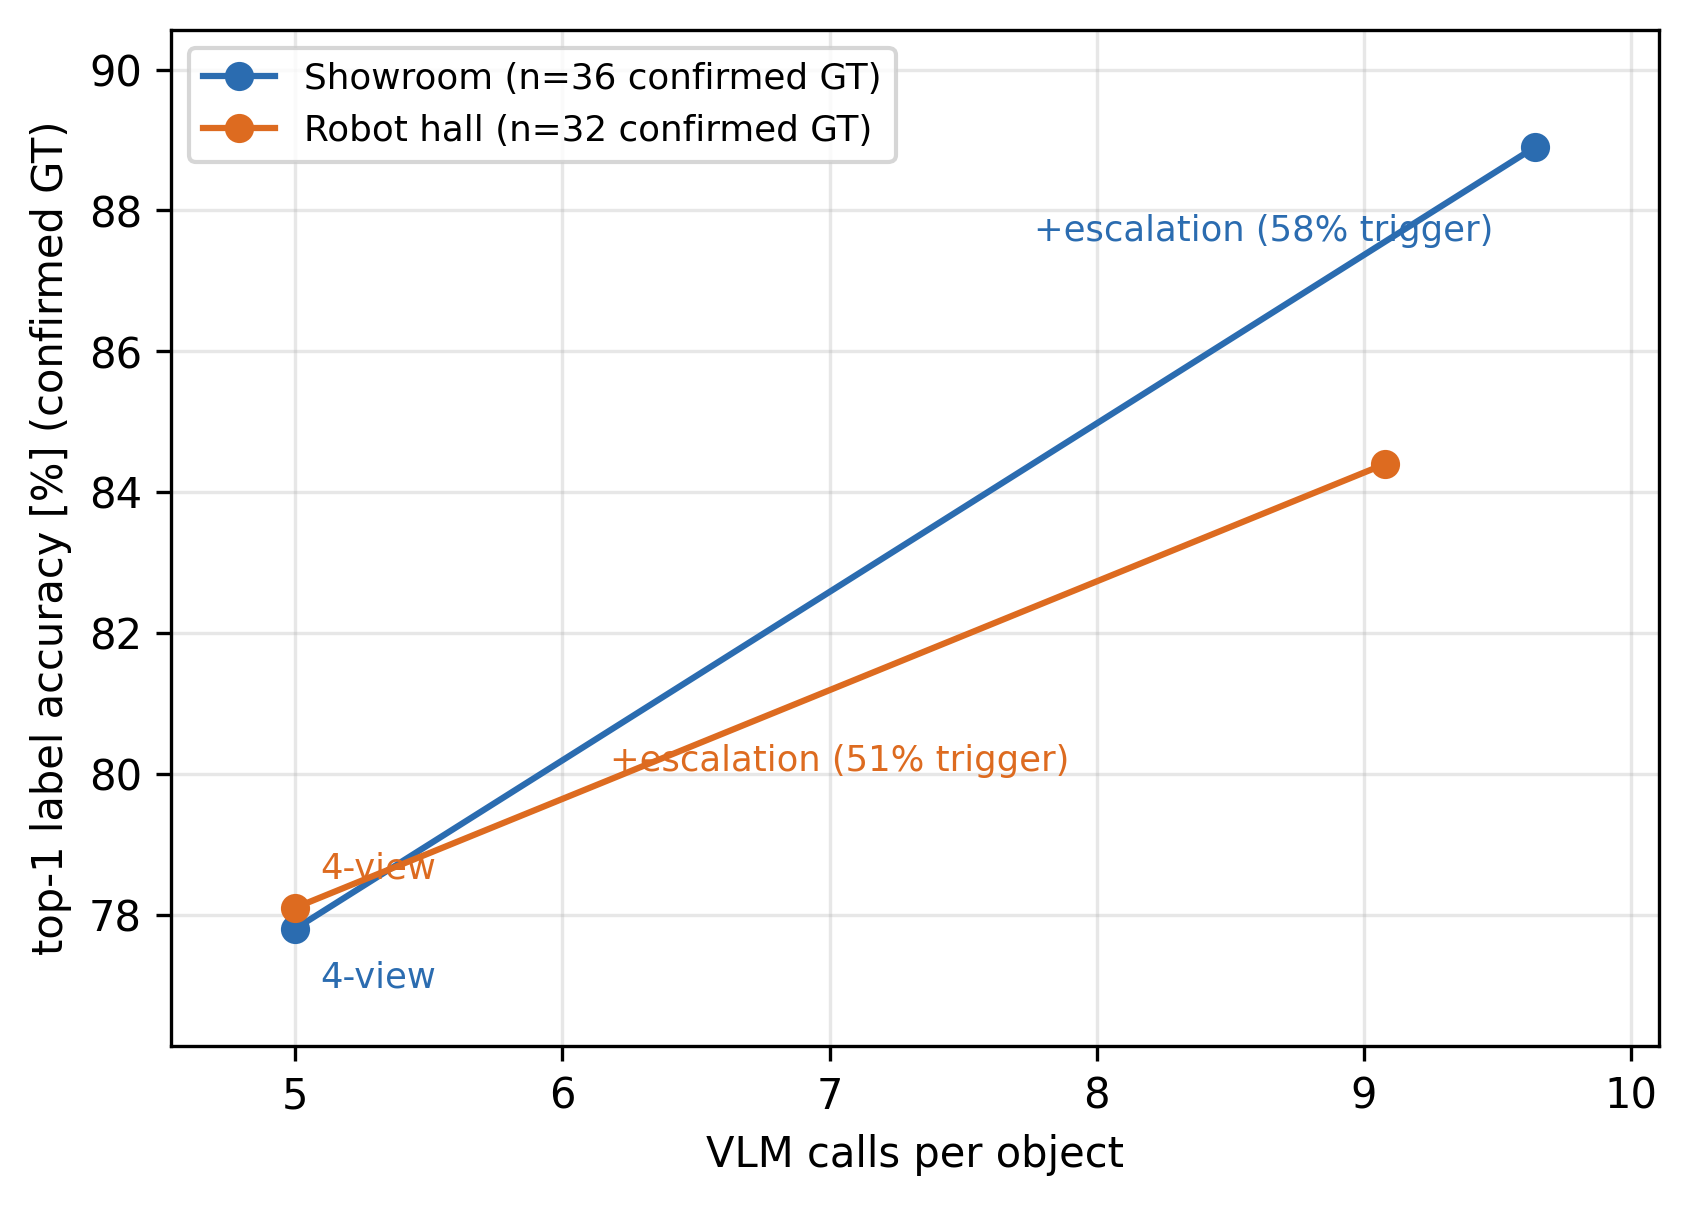
\includegraphics[width=0.85\linewidth]{figures/ele_fig6_escalation_cost.png}
\caption{Escalation accuracy--cost curves for both scenes.}
\label{fig:esccost}
\end{figure}

Precision alone understates what gating costs, so Table~\ref{tab:tierrf}
completes the tier picture with recall and $F_1$. The combined verified tier
reaches recall 0.722/0.781 on the two industrial scenes ($F_1$ 0.839/0.847)
but only 0.250 on the cafeteria, where the gate abstained on half of the
confirmed objects---the stress scene's segmentation failures surface as
recall, not as precision. Because the 0.6 share threshold gates status only,
its effect can be quantified exactly by re-scoring the stored votes at
alternative thresholds: sweeping 0.40--0.90 shows 0.6 sitting on a plateau
rather than a cliff, with $F_1$ maximized on a broad 0.45--0.65 band on both
industrial scenes and every 0.05 step moving at most one or two objects, so the
a priori 0.6 is retained rather than tuned post hoc.

\begin{table}[htbp]
\centering
\caption{Per-tier precision, recall, and $F_1$ on confirmed ground truth
(synonym-tolerant). The unverified row is the abstention tier.}
\label{tab:tierrf}
\small\setstretch{1.15}
\begin{tabular}{l l r r r r r}
\toprule
\textbf{Scene} & \textbf{Tier} & $n$ & $n_{\mathrm{conf}}$ & Prec. & Rec. & $F_1$ \\
\midrule
Showroom & verified (unanimous) & 21 & 19 & 1.000 & 0.528 & 0.691 \\
 & verified\_escalated & 8 & 7 & 1.000 & 0.194 & 0.326 \\
 & combined verified & 29 & 26 & 1.000 & 0.722 & 0.839 \\
 & unverified (abstained) & 21 & 10 & 0.600 & 0.167 & 0.261 \\
\midrule
Robot hall & verified (unanimous) & 25 & 18 & 0.944 & 0.531 & 0.680 \\
 & verified\_escalated & 16 & 9 & 0.889 & 0.250 & 0.390 \\
 & combined verified & 41 & 27 & 0.926 & 0.781 & 0.847 \\
 & unverified (abstained) & 10 & 5 & 0.400 & 0.062 & 0.108 \\
\midrule
Cafeteria & verified (unanimous) & 8 & 7 & 0.571 & 0.200 & 0.296 \\
 & verified\_escalated & 6 & 3 & 0.333 & 0.050 & 0.087 \\
 & combined verified & 14 & 10 & 0.500 & 0.250 & 0.333 \\
 & unverified (abstained) & 11 & 10 & 0.200 & 0.100 & 0.133 \\
\bottomrule
\end{tabular}
\end{table}

\subsection{Error Taxonomy and Class-Level Breakdown}
\label{subsec:exp-errors}

Four recurring error classes emerged (Figure~\ref{fig:taxonomy}):
(a)~\emph{structure-remnant phantoms}---soffit bands verified as keyboards,
eliminated upstream by the remnant filter; (b)~\emph{unanimous-but-wrong}---a
hanging chain unanimously verified as a door handle, partition fragments as
chairs, and at T3 a residual 7.4~m wall segment escalation-verified as a
staircase whose phantom label then propagated into a place name
(\texttt{staircase\_landing}), showing that place naming is verifier-bounded
too; a third case is the mirror image, in which the room's large wall-mounted
TV was geometrically detected yet left \texttt{unverified} while a small
co-located cluster was verified as a fire extinguisher the owner refuted;
(c)~\emph{clutter absorption}---a disassembled robot, a poster stand, and a
low-reflectance floor fan (674 points) each unanimously verified as
\texttt{clutter}: geometrically detected, semantically flattened; and
(d)~\emph{render ambiguity} $\rightarrow$ \texttt{unverified}, the intended
failure mode. Classes (b) and (c) motivate reporting verification as tiered
evidence rather than truth. Table~\ref{tab:classdist} disaggregates every
scene's ground truth into class families: robots are the worst family
everywhere they occur (0/4, 0/3, and 0/8 correct across the three
robot-bearing sets)---absorption, not misperception, since most land in
\texttt{clutter} or abstain---and displays and fixtures abstain heavily on the
showroom, exactly the render-ambiguous shapes the taxonomy predicts.

\begin{figure}[!htb]
\centering
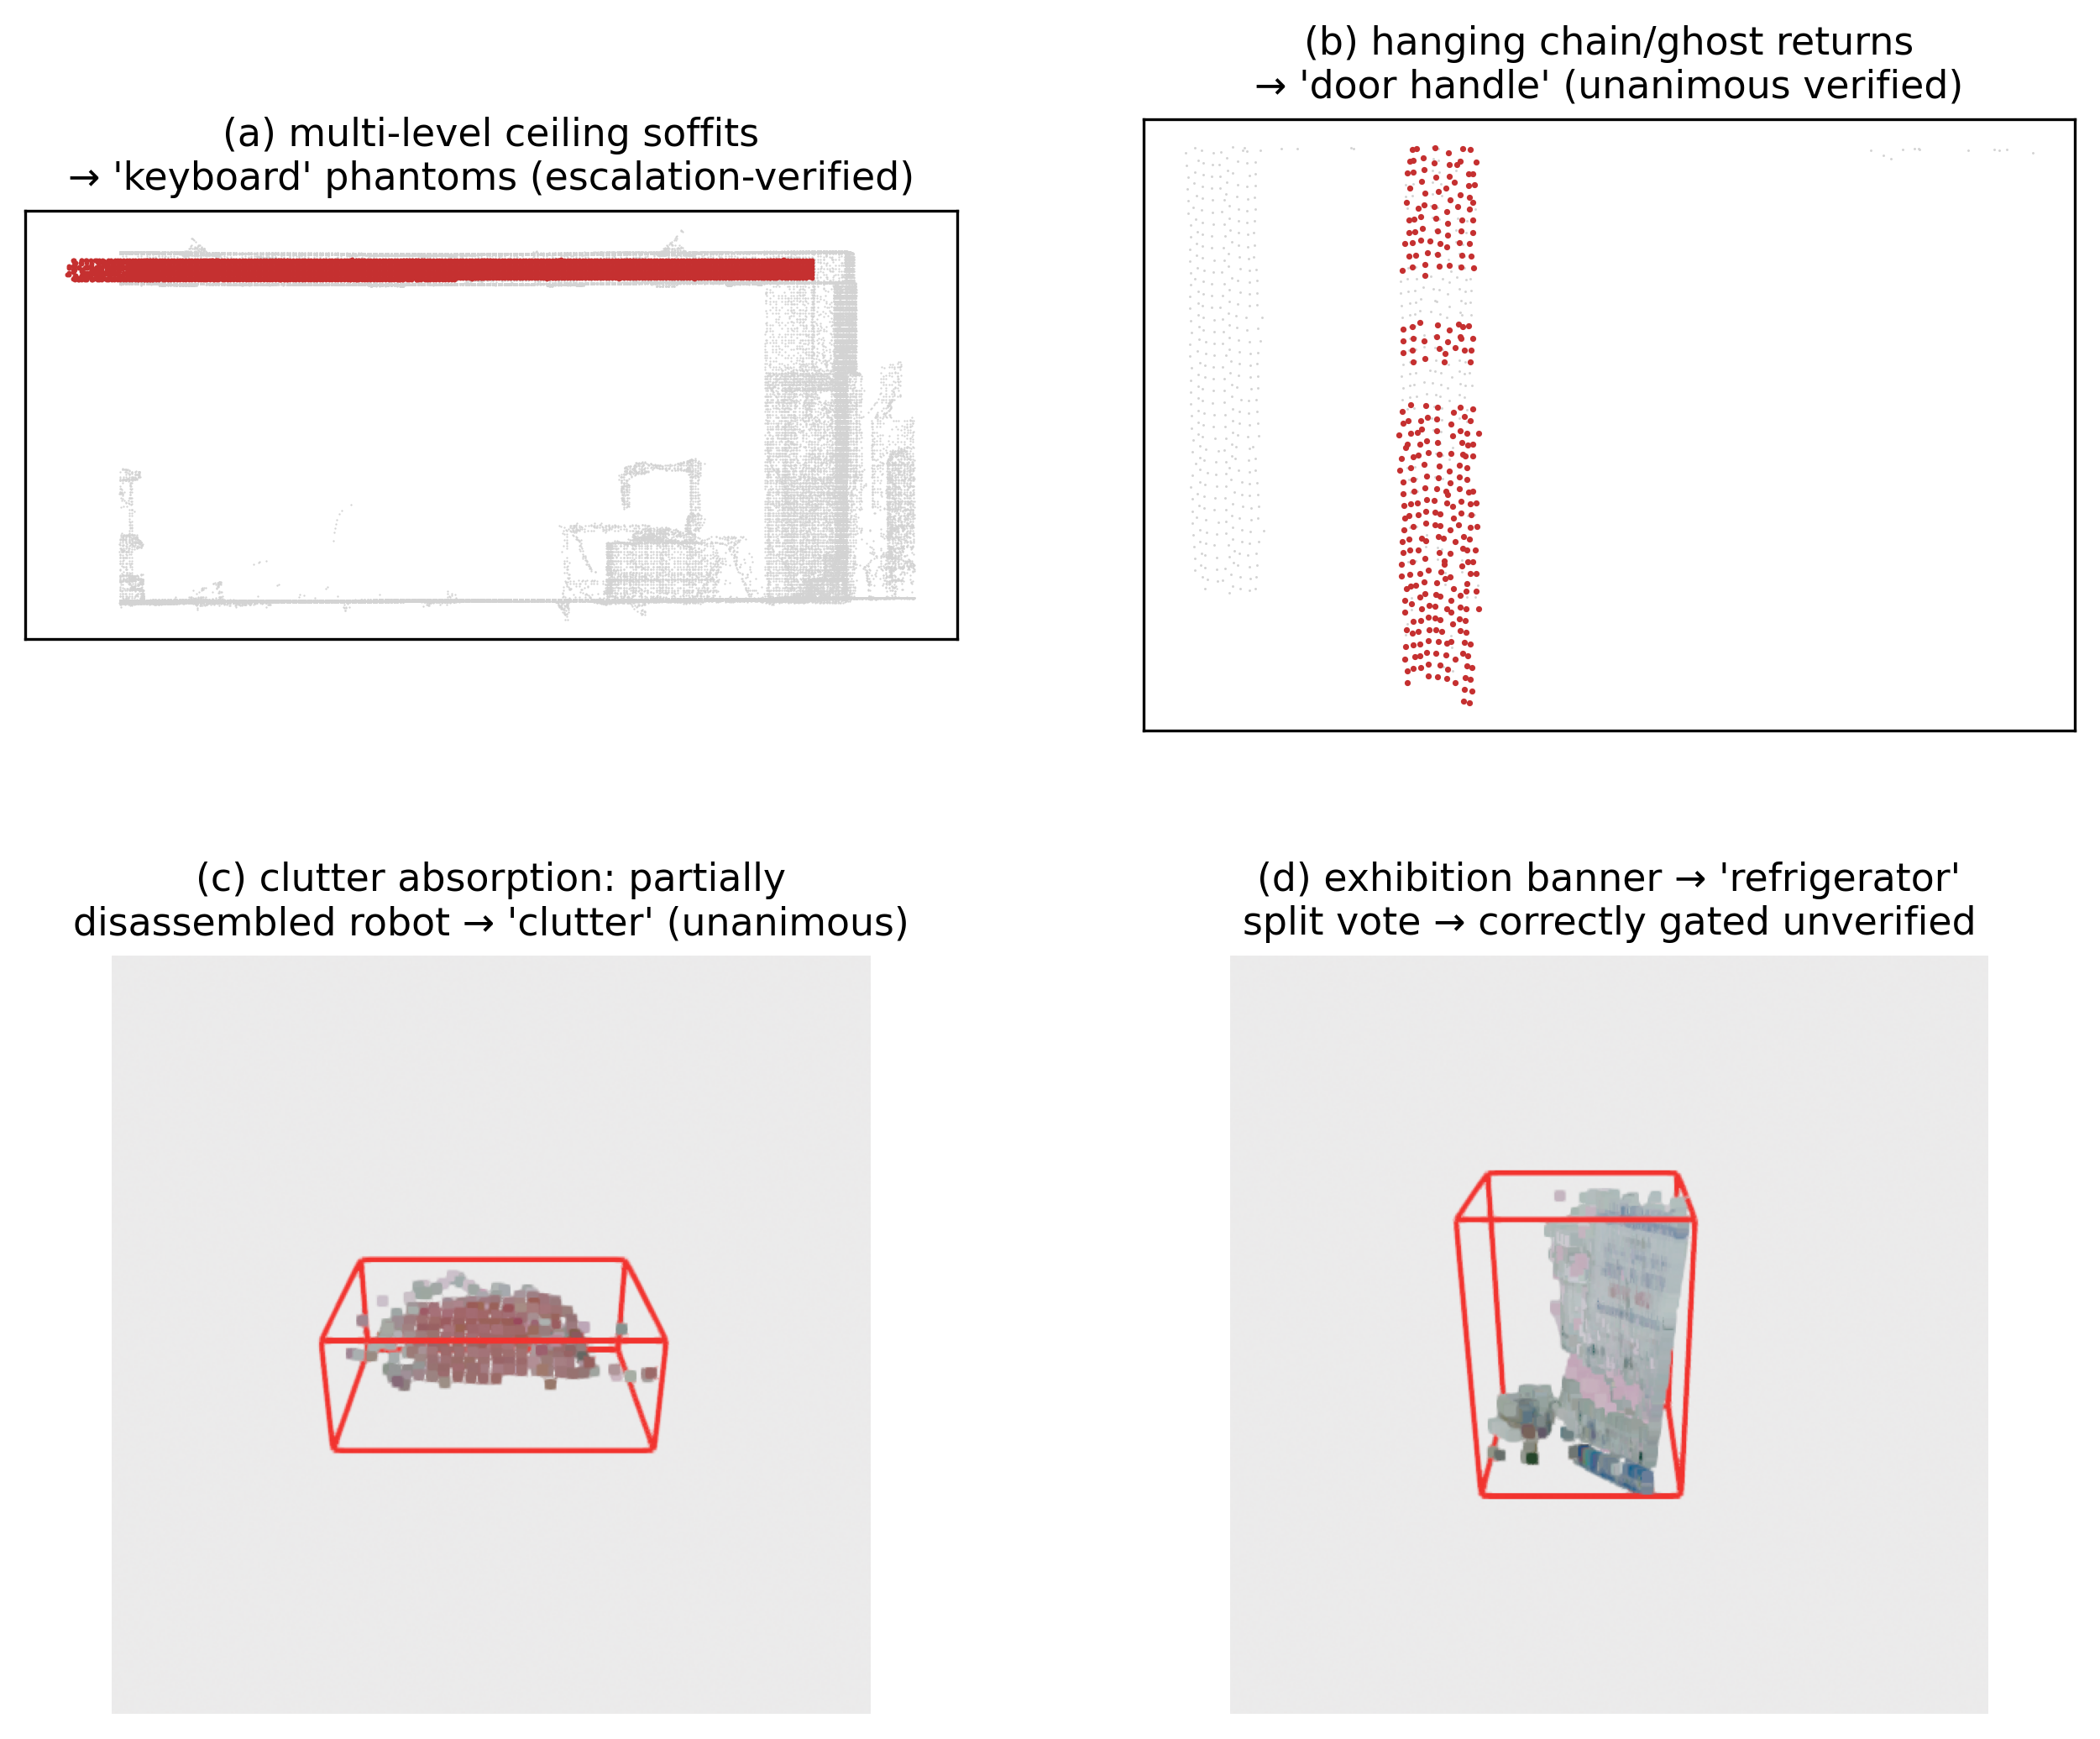
\includegraphics[width=0.9\linewidth]{figures/ele_fig10_error_taxonomy.png}
\caption{Verification error taxonomy: remnant phantom, unanimous-but-wrong,
clutter absorption, render ambiguity.}
\label{fig:taxonomy}
\end{figure}

\begin{table}[htbp]
\centering
\caption{Ground-truth object classes per scene, grouped into families, with
each object's verification outcome in the canonical run. ``Filtered'' =
excluded before scoring (structure artifact or out of room scope).}
\label{tab:classdist}
\small\setstretch{1.15}
\begin{tabular}{l l r r r r r}
\toprule
\textbf{Scene} & \textbf{Family} & GT & Corr. & Wrong & Unver. & Filt. \\
\midrule
Showroom (57-set) & seating & 5 & 4 & 1 & 0 & 0 \\
 & robots & 4 & 0 & 1 & 3 & 0 \\
 & displays/monitors & 5 & 0 & 0 & 5 & 0 \\
 & machines/electrical & 6 & 3 & 0 & 3 & 0 \\
 & furniture & 2 & 0 & 0 & 2 & 0 \\
 & fixtures & 6 & 0 & 0 & 6 & 0 \\
 & structure-noise & 7 & 0 & 0 & 0 & 7 \\
 & clutter/unknown & 22 & 20 & 0 & 2 & 0 \\
 & \emph{total} & 57 & 27 & 2 & 21 & 7 \\
\midrule
Robot hall (det) & seating & 5 & 4 & 0 & 1 & 0 \\
 & robots & 3 & 0 & 1 & 2 & 0 \\
 & displays/monitors & 1 & 0 & 0 & 0 & 1 \\
 & machines/electrical & 1 & 0 & 0 & 0 & 1 \\
 & furniture & 2 & 0 & 0 & 0 & 2 \\
 & fixtures & 8 & 3 & 1 & 4 & 0 \\
 & structure-noise & 8 & 0 & 0 & 1 & 7 \\
 & clutter/unknown & 53 & 25 & 7 & 2 & 19 \\
 & \emph{total} & 81 & 32 & 9 & 10 & 30 \\
\midrule
Cafeteria & seating & 10 & 1 & 4 & 5 & 0 \\
 & machines/electrical & 1 & 1 & 0 & 0 & 0 \\
 & furniture & 1 & 0 & 1 & 0 & 0 \\
 & fixtures & 5 & 0 & 1 & 4 & 0 \\
 & structure-noise & 3 & 0 & 0 & 0 & 3 \\
 & clutter/unknown & 8 & 4 & 2 & 2 & 0 \\
 & \emph{total} & 28 & 6 & 8 & 11 & 3 \\
\midrule
T3 re-scan (owner GT) & seating & 5 & 2 & 2 & 1 & 0 \\
 & robots & 8 & 0 & 6 & 2 & 0 \\
 & displays/monitors & 2 & 0 & 1 & 1 & 0 \\
 & machines/electrical & 4 & 0 & 4 & 0 & 0 \\
 & furniture & 4 & 0 & 3 & 1 & 0 \\
 & fixtures & 4 & 0 & 2 & 2 & 0 \\
 & structure-noise & 9 & 0 & 6 & 3 & 0 \\
 & clutter/unknown & 5 & 4 & 0 & 0 & 0 \\
 & \emph{total} & 41 & 6 & 25 & 10 & 0 \\
\bottomrule
\end{tabular}
\end{table}

\section{Owner Audit and Corrective Feedback}
\label{sec:exp-owner}

The preceding section measured what the pipeline believes; this one measures
what the room's occupant knows, and how that knowledge feeds back into the
graph. The room's occupant exhaustively labeled all 41 T3 clusters. Of the 31
verified-tier clusters, 6 were correct, 13 were real objects flattened to
\texttt{clutter}, 6 were structure-noise phantoms, 2 carried a wrong specific
label, and 3 were multi-object merges. The cause of the absorption is
identifiable: the room is a robotics testbed (mobile robots, manipulators,
charging stations, a disinfection robot), and none of these classes exist in
the classifier vocabulary. Three audit-driven mitigations follow (layers 4--5 of
Section~\ref{sec:corrective}). \emph{(i) Hybrid structure filter:} registering
every cluster against the exploration occupancy grid removes structure noise at
12/12 recall with 3 false positives (thin wall-flush real objects: a cabinet
leg, a poster stand); crucially, the wall-flush monitor bank survives, because
its 1.8~m height and per-segment depth separate it from the 3.2~m
floor-to-ceiling wall band that plane removal missed
(Figure~\ref{fig:structfilter}). \emph{(ii) Recovery re-verification:}
re-asking the verifier with \texttt{clutter} treated as unidentified plus a
candidate shortlist recovered 4 specific types at 4/5 precision; injecting
site vocabulary (robot classes) as candidates doubled recovery (9 correct) but
halved precision (8 wrong) through candidate anchoring---the TV became a
``conveyor belt'' when the shortlist ranked it first. \emph{(iii) Agreement
gating:} adopting a recovered label only when both passes agree, or when a
pass agrees with the cluster's own base label, yields five adoptions at 5/5
precision (two chairs, an office chair, a machine, and the TV) and resurrects
no owner-refuted phantom. Domain knowledge helps recall; only agreement makes
it safe. Refutations, corrections, and adopted labels were applied as a graph
revision through the same upsert mechanism as a re-scan: eight phantoms leave
the graph, five recovered types land, the TV becomes its region's key object,
the relation layer sheds nine noise-anchored edges, and re-deriving ring codes
heals the place layer end to end---the phantom-derived
\texttt{staircase\_landing} becomes \texttt{display\_briefing\_area}, the
keyboard-derived \texttt{workstation\_area} becomes \texttt{machine\_area},
and the seating region's recovered chairs turn
\texttt{cluttered\_seating\_area} into \texttt{seating\_area}. Owner feedback
thus propagates through all three layers of the model: object, relation, and
place.

\begin{figure}[!htb]
\centering
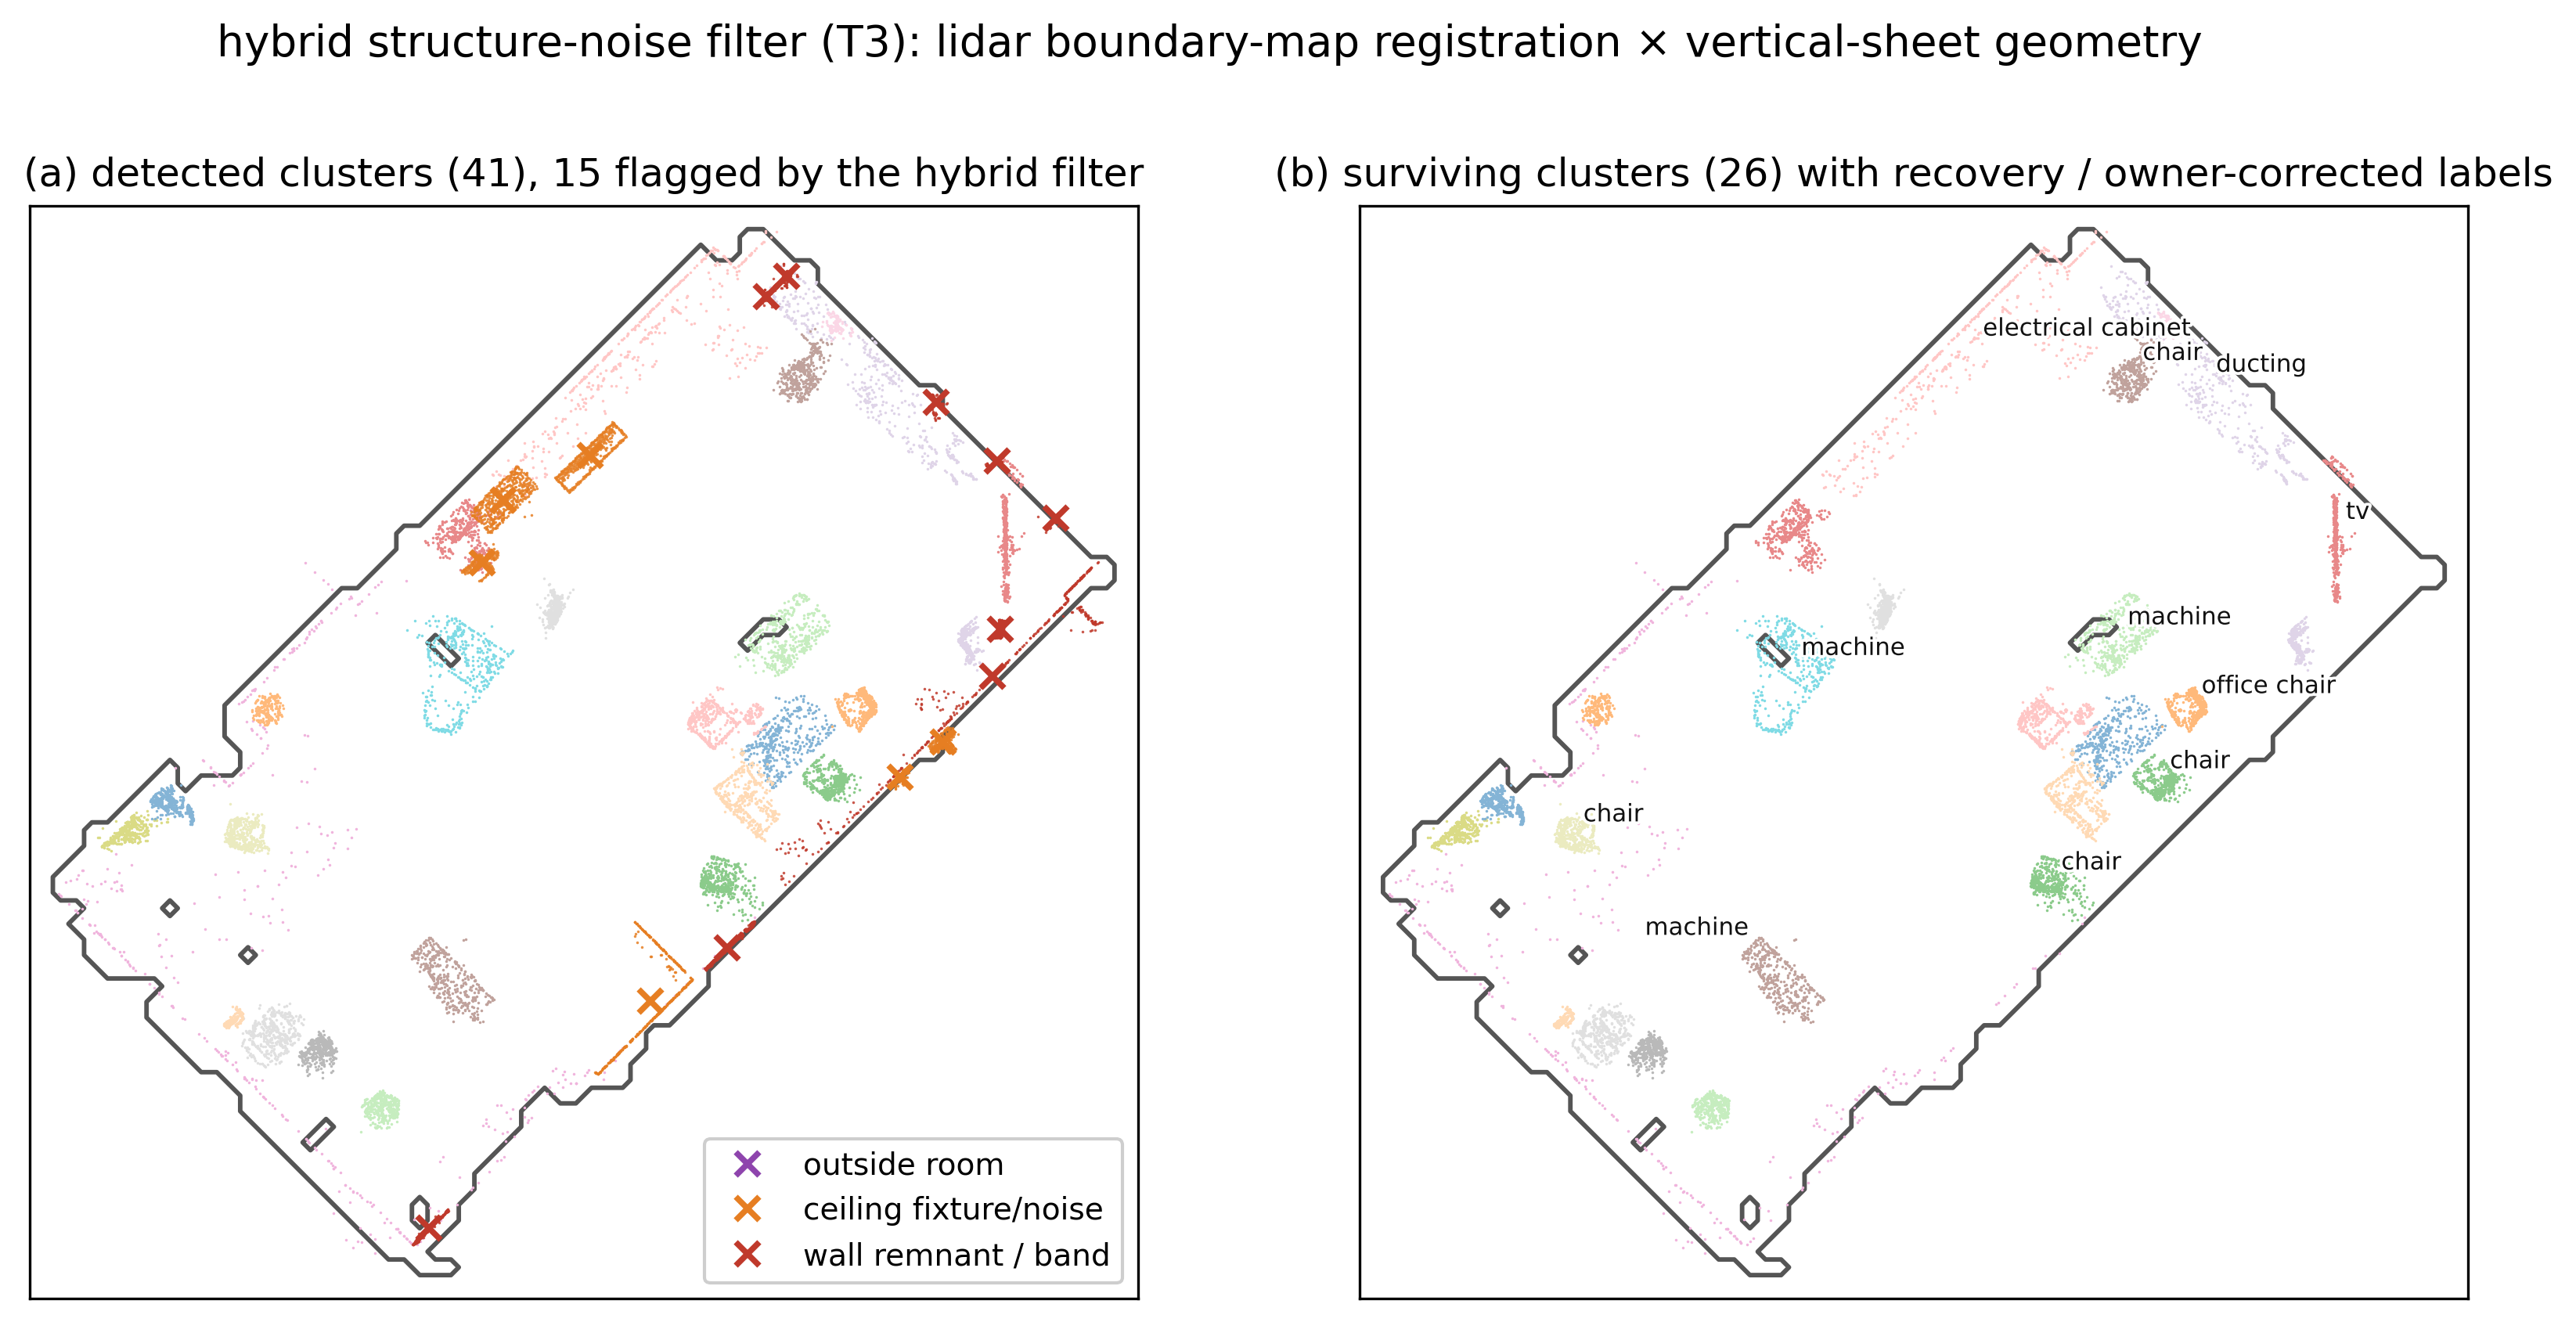
\includegraphics[width=\linewidth]{figures/ele_fig14_structure_filter.png}
\caption{Hybrid structure-noise filter on the T3 epoch. (a)~All 41 detected
clusters; the 15 flagged ones are colored by rule (wall remnant/band, ceiling
fixture/noise, outside the room boundary). (b)~The 26 survivors with recovery
and owner-corrected labels; the wall-flush monitor bank and wall-mounted
equipment survive.}
\label{fig:structfilter}
\end{figure}

Extending the audit loop through nine further revisions shows owner feedback
operating in all four directions the model supports. \emph{Restoration}: an
object the owner had refuted as absent was later declared present again (the
room changed between audits); a color-seeded carve at the owner-given corner
recovered a 319-point red cylinder that two-pass verification typed
\texttt{fire extinguisher}---the original failure was segmentation, not
classification, and owner ground truth is itself time-variant.
\emph{Refutation}: a raw-condition ensemble find was refuted as wall paint, the
halo around the hole left by the glossy black screen of the wall TV.
\emph{Label correction}: the correlated-bias tables and a poster stand were
corrected in place with the VLM verdict preserved in provenance.
\emph{Attribute correction}: wall-remnant clutter was marked immovable. The
live graph has accumulated thirteen revisions through the same mechanism, and
every transition, including the mistakes it corrects, is reconstructible from
node histories.

\section{Knowledge-Grounded Query Evaluation}
\label{sec:exp-query}

Four conditions are evaluated over identically constructed per-scene query
sets---48 items on the showroom, 32 on the robot hall (symbolic, explicit,
scene-level, and trap questions): (1)~\emph{LLM-only} (an unverified Stage-A
object dump, no verification), (2)~\emph{ungated KG}, (3)~\emph{verified-only
KG} (unverified nodes removed), and (4)~\emph{gated KG} (unverified retained
but structurally demoted). Each scene carries four trap questions about
objects that do not exist as labeled; on the showroom all four target
unverified-label phantoms, on the robot hall two target an unverified-label
phantom and two an \emph{escalation-verified} phantom, probing the gate's
verifier-quality bound. On the showroom (Table~\ref{tab:query},
Figure~\ref{fig:query}), grounding alone lifts accuracy from 52.1\% to 81.2\%
but blocks no traps; removing unverified content blocks all four traps at a
steep recall price (12 abstentions, 58.3\%); the gated condition is the balance
point---83.3\% with 3/4 traps blocked. The two leaks are mechanistically
distinct: on the showroom, one count-phrased trap slipped through the
quarantine itself, the model tallying a demoted node by reading its
\texttt{failedCandidateType} field; on the robot hall, the keyboard phantom is
escalation-verified, so it passes any status-based gate---gating is bounded by
verifier quality. The robot hall reproduces the ordering at lower absolute
levels because its end-to-end label errors propagate into every grounded
condition. At $n=48$/32 questions the gated-versus-ungated accuracy gap is a
single question on each scene, so the benchmark is diagnostic rather than
powered for significance; the case for gating rests on the mechanisms the
benchmark isolates---trap blocking, the abstention structure, and the direction
of the hallucination change---and on the mission-level consequences of
Section~\ref{sec:exp-missions}.

\begin{table}[htbp]
\centering
\caption{Query benchmark, four conditions. Acc.\ = accuracy, Hall.\ =
hallucination rate, Traps = trap questions blocked (of 4), Abst.\ =
abstentions. An abstention counts against accuracy but is not a hallucination.
Source: \emph{Electronics}~\cite{kim2026electronics}.}
\label{tab:query}
\small
\begin{tabular}{l c c c c c c c c}
\toprule
 & \multicolumn{4}{c}{\textbf{Showroom ($n=48$)}} & \multicolumn{4}{c}{\textbf{Robot hall ($n=32$)}} \\
\textbf{Condition} & Acc. & Hall. & Traps & Abst. & Acc. & Hall. & Traps & Abst. \\
\midrule
LLM-only & 52.1\% & 20.8\% & 2/4 & 13 & 50.0\% & 37.5\% & 4/4 & 4 \\
Ungated KG & 81.2\% & 18.8\% & 0/4 & 0 & 56.2\% & 43.8\% & 0/4 & 0 \\
Verified-only KG & 58.3\% & 16.7\% & 4/4 & 12 & 46.9\% & 40.6\% & 2/4 & 4 \\
Gated KG (proposed) & \textbf{83.3\%} & \textbf{16.7\%} & 3/4 & 0 & \textbf{59.4\%} & \textbf{40.6\%} & 2/4 & 0 \\
\bottomrule
\end{tabular}
\end{table}

\begin{figure}[!htb]
\centering
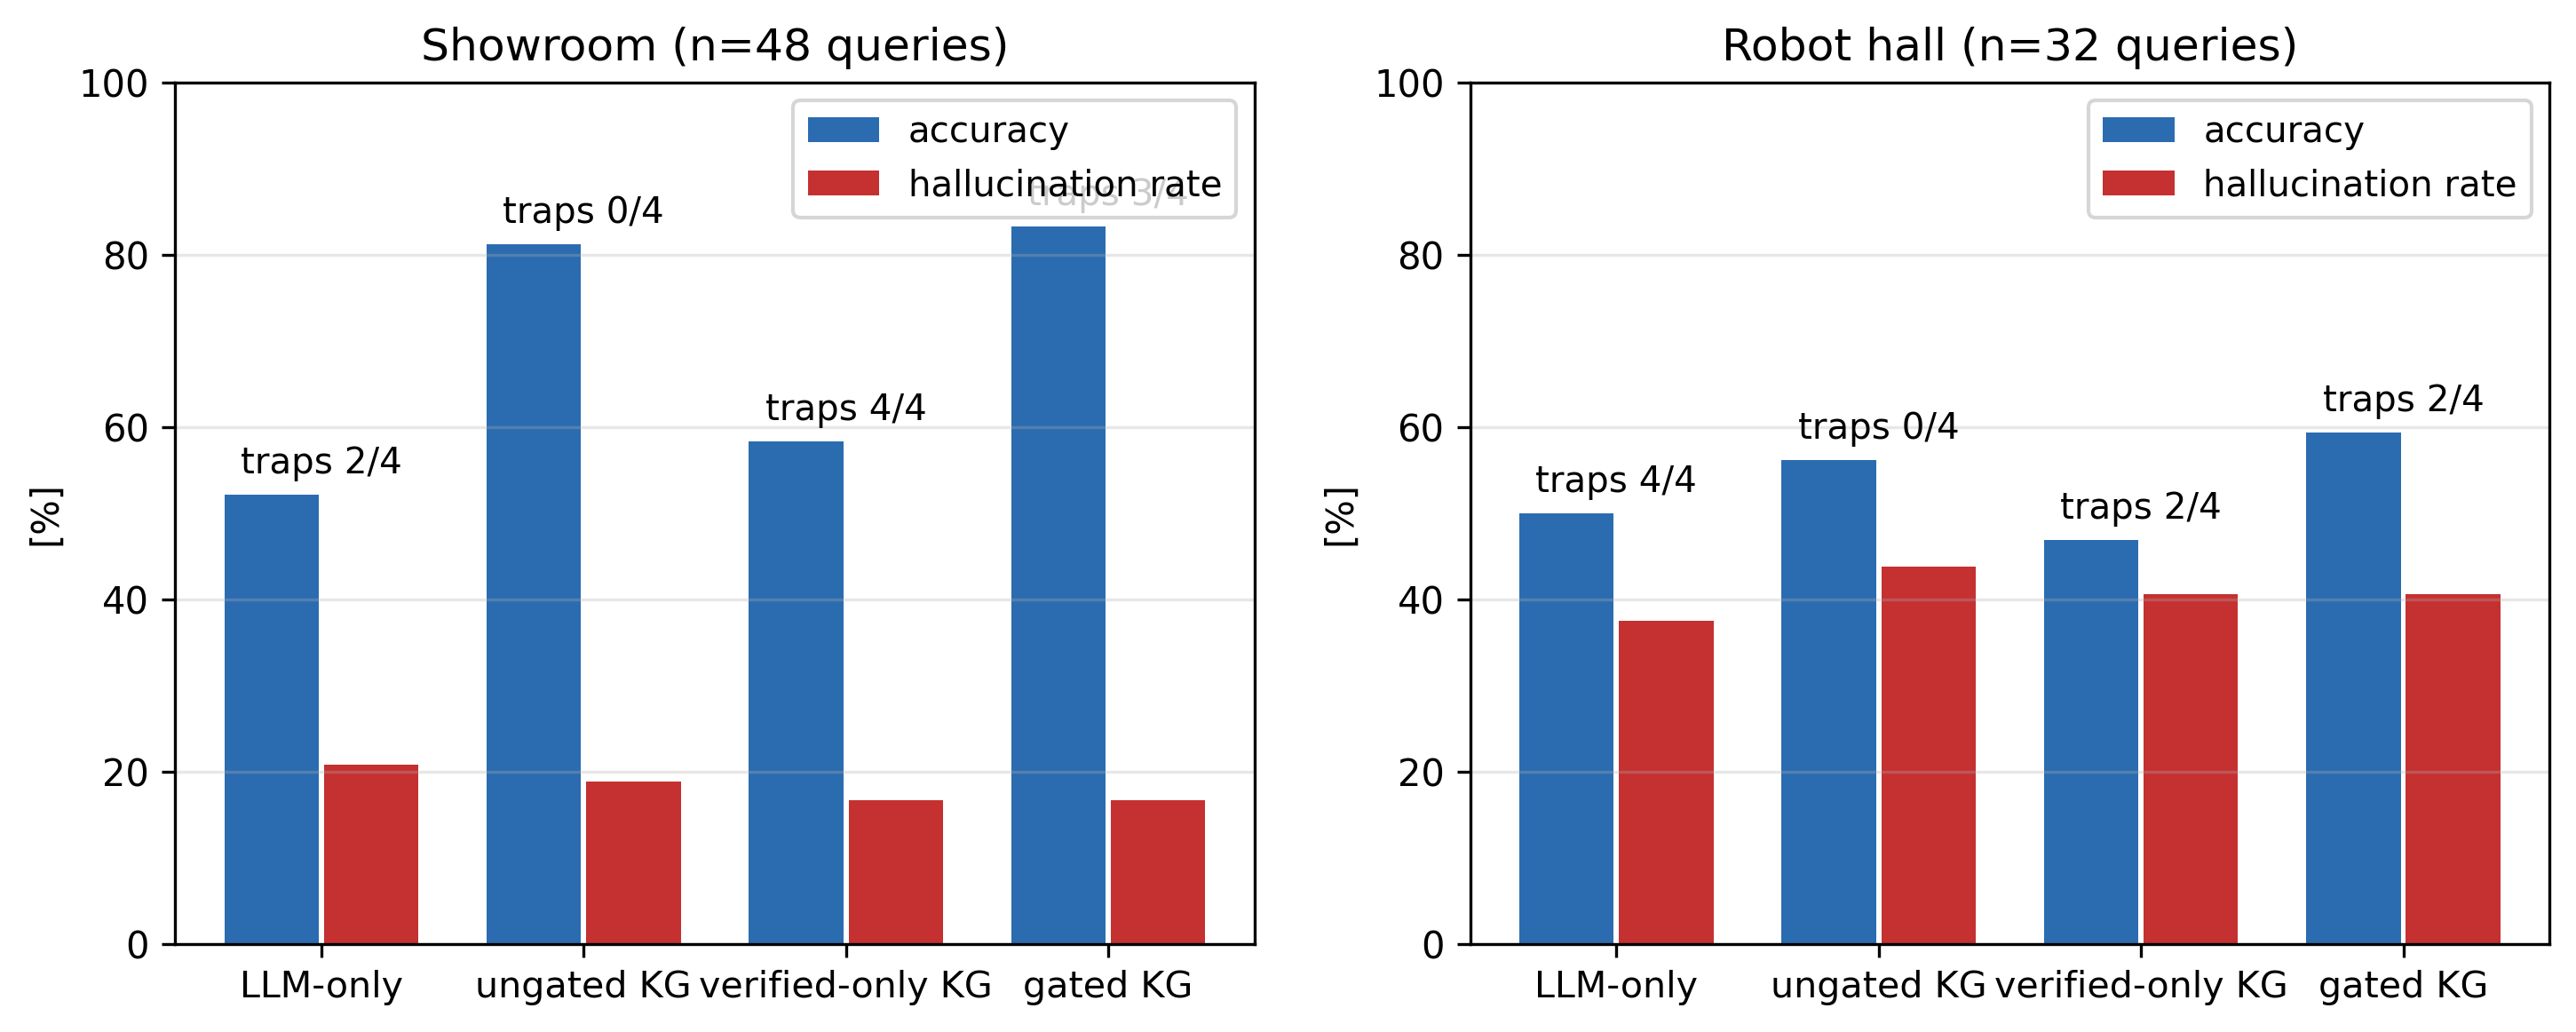
\includegraphics[width=0.9\linewidth]{figures/ele_fig7_query_benchmark.png}
\caption{Four-condition query benchmark with trap-question panel.}
\label{fig:query}
\end{figure}

\section{Incremental Update Evaluation}
\label{sec:exp-update}

\paragraph{Synthetic scenarios.}
Controlled edits of the room-scoped robot hall isolate matcher behavior
(Figure~\ref{fig:update}): (A)~unchanged repeat: 55/55 nodes carried, zero VLM
calls, zero identity switches; (B)~move: 1/1 moved with ID preserved;
(C)~remove+insert: exact absent/insert classification; (D)~occlusion: at 20\%
crop both affected objects still match, at 40\% matching fails into 2
false-absents + 2 false-news---the matcher's quantified breaking point. On the
combined-edit re-scan (move, insertion, and removal applied together),
selective re-verification re-ran Stage~B on only the two changed clusters: 26
of 822 VLM calls, \$0.23 versus \$7.37 for a full re-verification---3.1\% of
rebuild cost, and 0\% for scenario~A. The claim is scoped precisely: the 3.1\%
figure comes from a controlled same-quality re-scan where unchanged clusters
reproduce byte-identically; on the real T2$\rightarrow$T3 transition the scan
protocol itself changed, no cluster hash matched, and the epoch paid full
verification cost (\$3.54 for 41 clusters).

\begin{figure}[!htb]
\centering
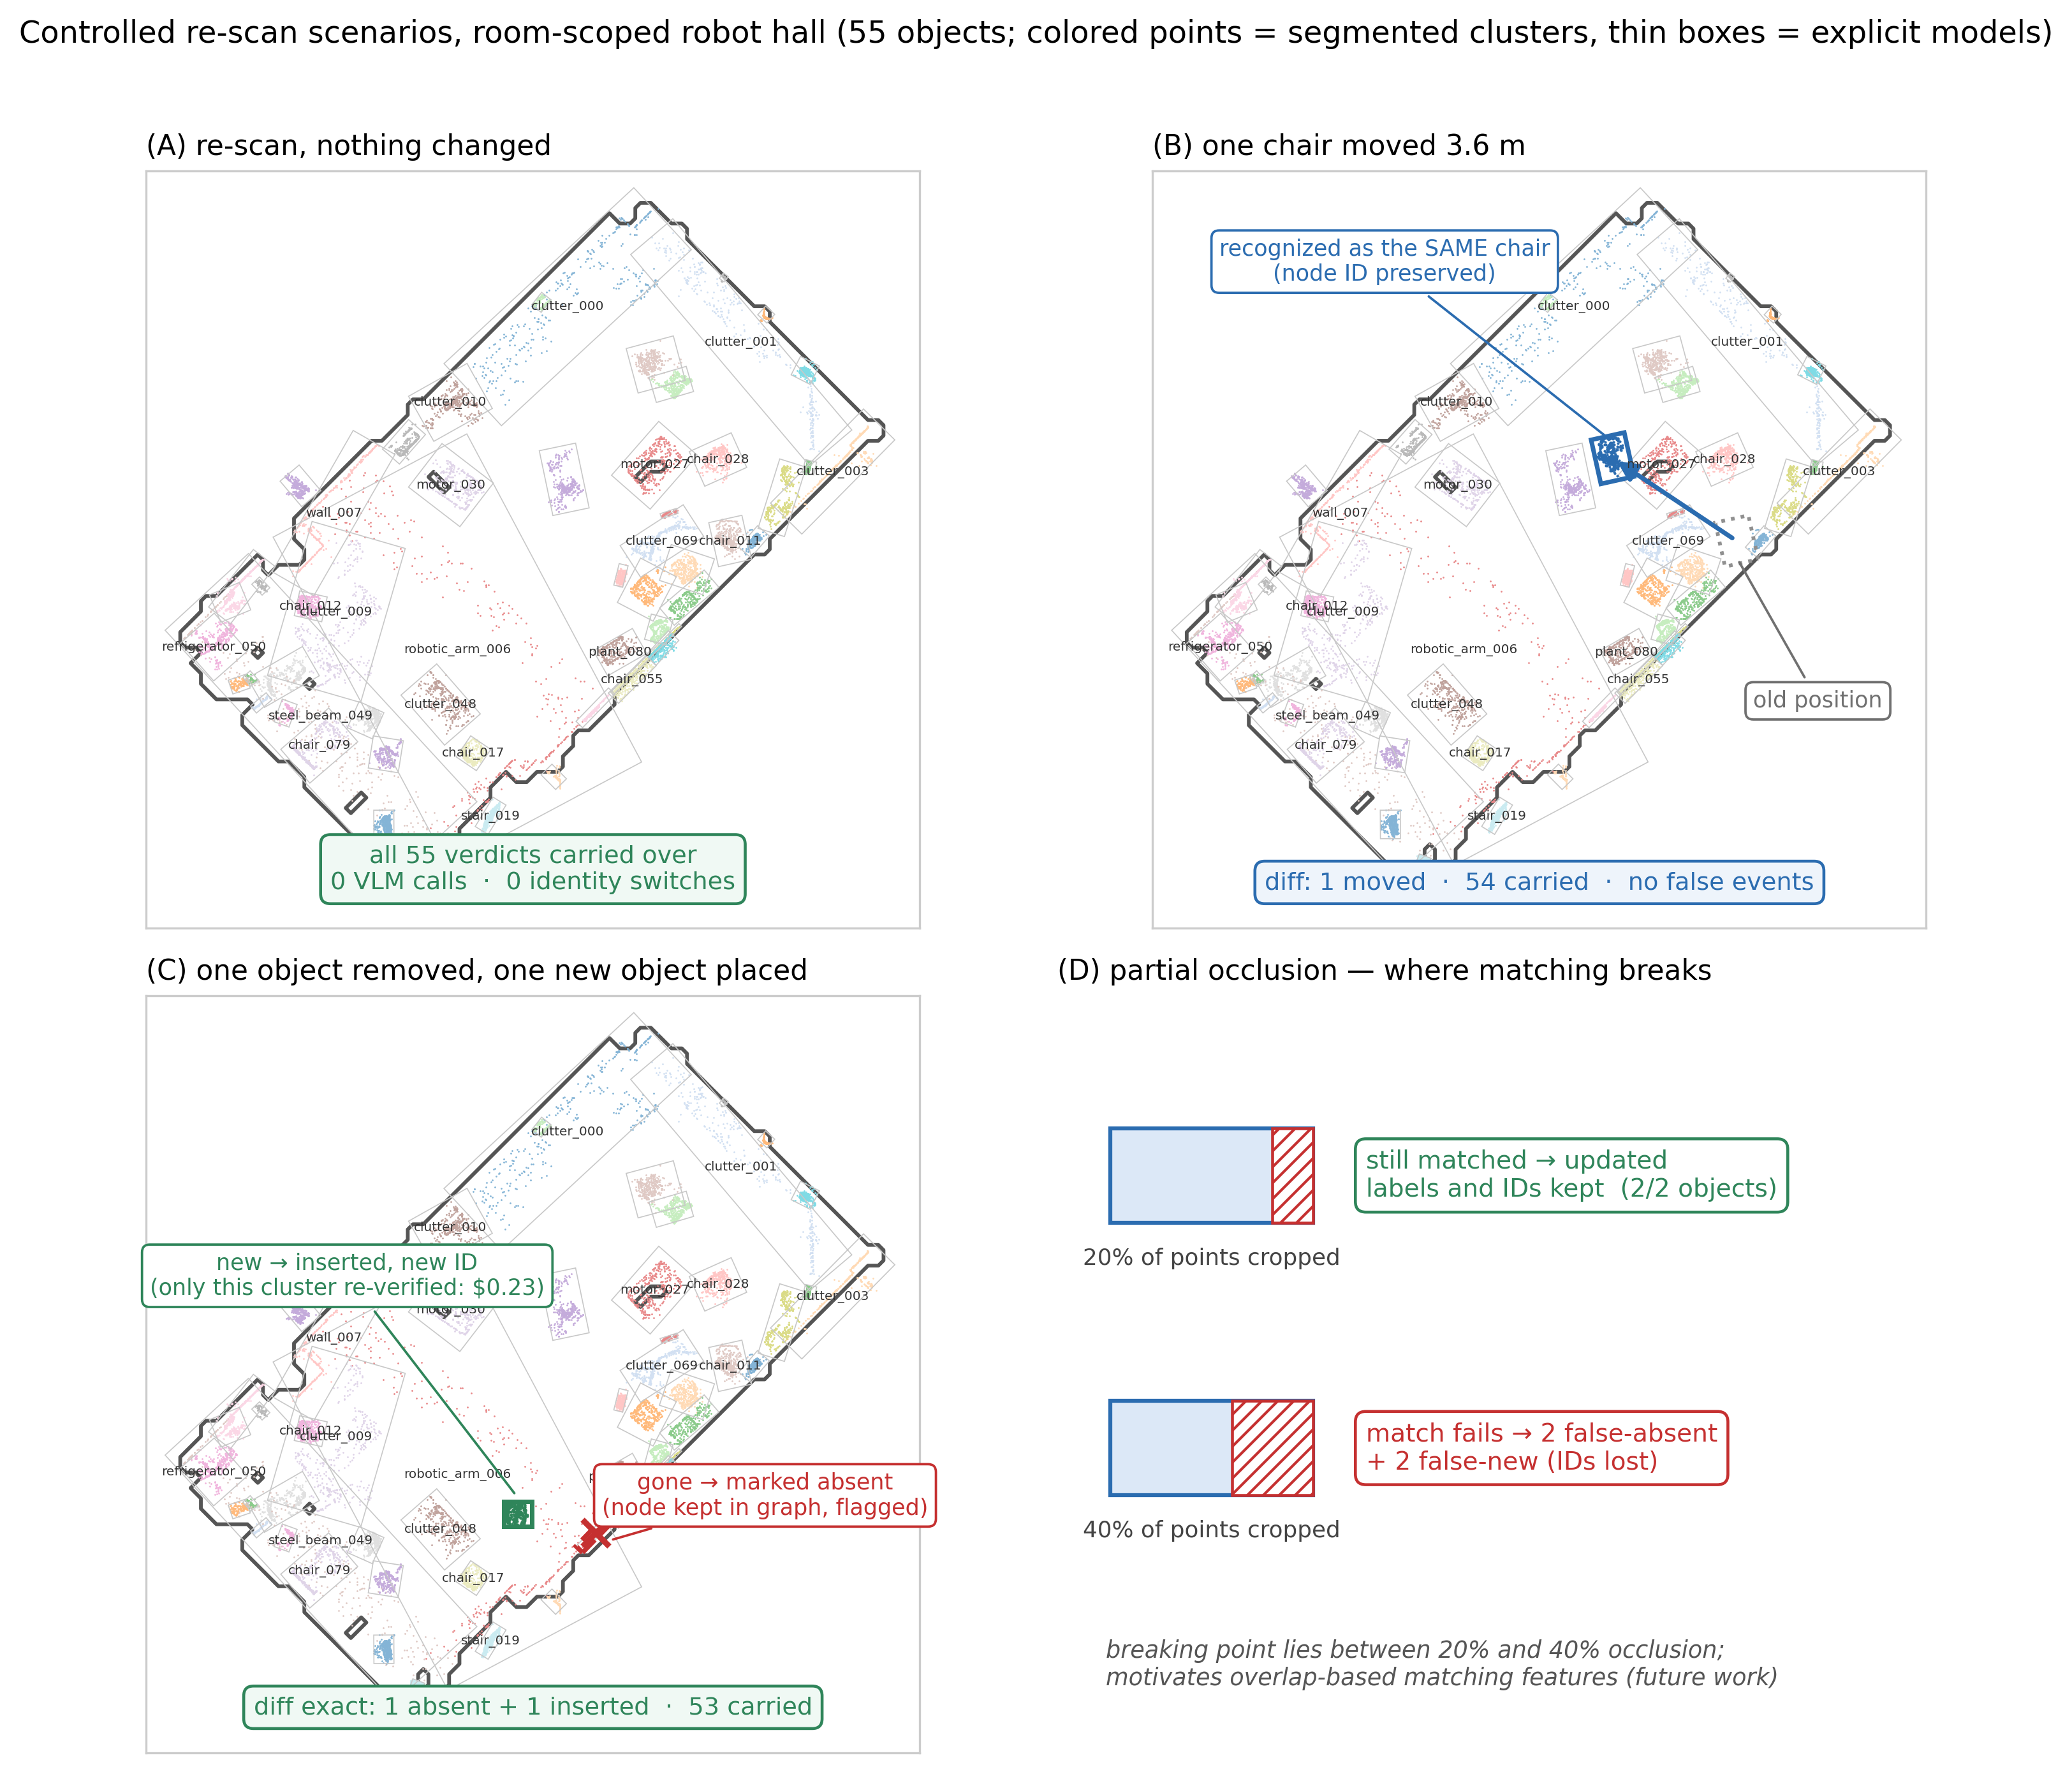
\includegraphics[width=0.9\linewidth]{figures/ele_fig8_incremental_update.png}
\caption{Controlled re-scan scenarios A--D (room-scoped robot hall, 55
objects), top-down view; each edited object is annotated with the matcher's
decision. (A)~A repeat scan carries all 55 verdicts at zero VLM cost. (B)~A
3.6~m chair move is classified \texttt{moved} with its node ID preserved.
(C)~A removed object is marked \texttt{absent} and a newly placed object is
\texttt{inserted}; only the insertion is re-verified. (D)~Partial occlusion:
both cropped objects still match at 20\%, but at 40\% matching fails.}
\label{fig:update}
\end{figure}

\paragraph{Real three-epoch study.}
The three epochs form a real update sequence: T1 (manual, June) $\rightarrow$
T2 (exploration, early July) $\rightarrow$ T3 (99.6\%-coverage exploration
with a controlled-change protocol, late July). Cross-epoch registration is
fully automatic (FPFH~\cite{rusu2009fpfh}+RANSAC then ICP~\cite{besl1992icp};
5.1~cm RMSE for T1$\rightarrow$T2, 4.2~cm for T3$\rightarrow$T2). The
T1$\rightarrow$T2 diff records the room's exhibition-to-test-hall
reorganization (updated 4 / moved 3 / inserted 48 / absent 31; among the moves,
a fire extinguisher displaced 3.0~m) and motivated the generic-type exclusion
in the move pass. The T2$\rightarrow$T3 diff (matched 9 / moved 1 / inserted 31
/ absent 45, Figure~\ref{fig:epochs}) sits on top of measured natural drift:
only 65\% of in-room object geometry is mutually supported at 10~cm between the
two scans, taken two weeks apart. To score the real transitions without circular
reference to the matcher, an independent correspondence reference was built by
bidirectional point overlap between epochs (4 strong and 6 partial static
pairs for T1$\rightarrow$T2, 7 strong and 5 partial for T2$\rightarrow$T3).
Matching accuracy on strong pairs is 2/4 and 4/7; \textbf{identity switches
are zero on both transitions}---every miss is a fragmentation error in which
re-segmentation changed an extent beyond the 30\% tolerance, so the object was
marked absent and re-inserted under a new ID, never associated with the wrong
object. Strict false-new and false-absent counts are 2/2 and 3/3, and all
three recorded \texttt{moved} claims are consistent with the reference (the
chair move is additionally owner-confirmed). Against the controlled-change
protocol, the system detected 2/2 physical changes at geometry level: the
moved chair is the epoch's only \texttt{moved} node (0.64~m, ID preserved
since T1), and the introduced floor fan was correctly \texttt{inserted} but
typed \texttt{clutter}. The fire extinguisher, pump, industrial robot, and
several chairs retain their minted IDs through both reorganizations, and the
place layer re-derives per-epoch names on the same regions (exhibition-era
\texttt{machine\_access\_area} $\rightarrow$ test-era
\texttt{machine\_operator\_station}) at about \$0.03 per epoch.

\begin{figure}[!htb]
\centering
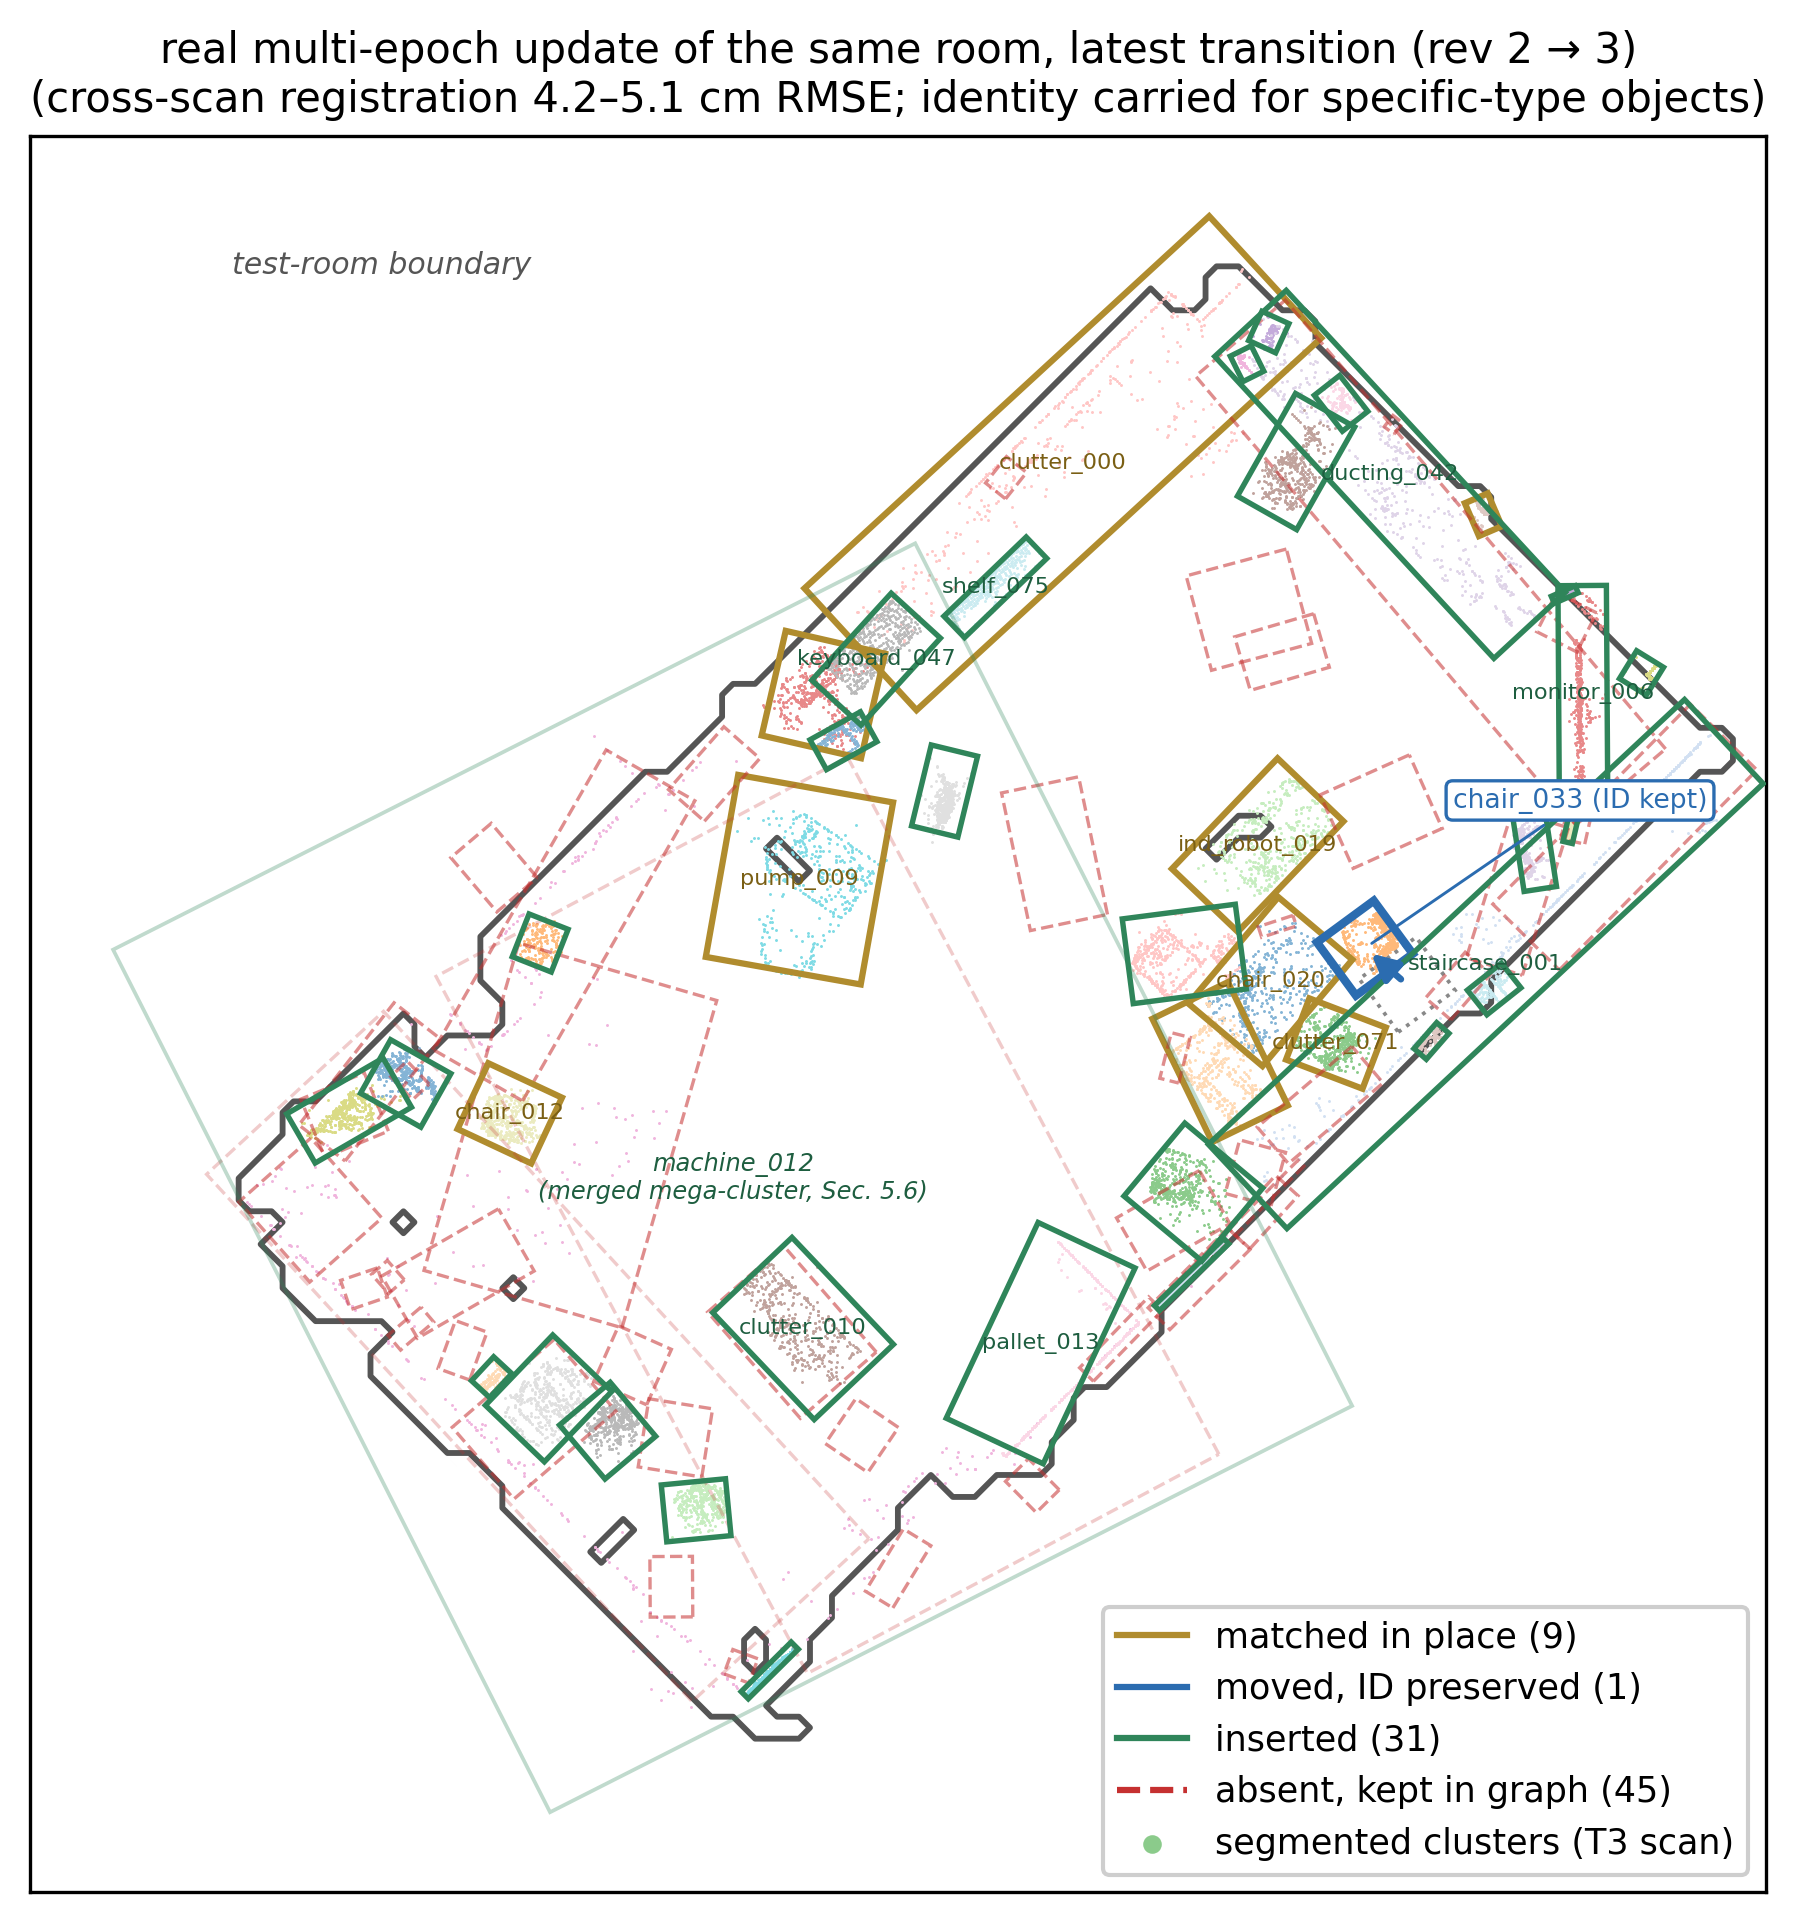
\includegraphics[width=0.9\linewidth]{figures/ele_fig9_two_epoch_update.png}
\caption{Real multi-epoch update, latest transition (T2$\rightarrow$T3),
top-down view: yaw-rotated node footprints colored by diff state (matched,
moved with ID preserved, inserted, absent). Oversized footprints of merged
mega-clusters are faded.}
\label{fig:epochs}
\end{figure}

\section{Retrospective End-to-End Replay}
\label{sec:exp-endtoend}

After the corrective machinery stabilized, the entire pipeline was re-run from
the raw T3 scan with no owner input at execution time and scored against the
live knowledge graph---by then a 46-object inventory embodying every owner
restoration, refutation, and correction. Because the corrective mechanisms were
developed from failures observed in this same environment, this is a
retrospective replay on the development scene, not an independent
generalization test: an independent \emph{run} on a non-independent
\emph{scene}. The cafeteria is the only scene independent in both senses, and
one corrective layer transfers mechanically to it: applying the hybrid
structure filter to the cafeteria with its T3 rules frozen flags both
ceiling-noise clusters with zero false positives, while the seven carpet
floor-noise clusters fall outside its rule families entirely.
Table~\ref{tab:layers} reports cumulative geometric recall as each automated
layer is enabled. The verified path alone recovers 28\%; diffuseness-gated
re-splitting nearly doubles it; the wall-compound gate (which self-triggers on
the monitor wall) and the structure-condition ensemble bring automated recall
to 85\%. Type accuracy saturates far lower ($\sim$31\% of recalled
objects)---the label bottleneck is the correlated verifier bias, and closing
it is precisely the owner layer's role. For calibration within the lineage's
own reporting style, DK-SMF reports 78--81\% detection accuracy against
predefined ground-truth objects in its RGB-D environments~\cite{joo2025dksmf};
the 85\% here is measured against an owner-audited inventory that includes
partially scanned and wall-flush objects, though the sensing modality and
ground-truth protocols differ. Each added layer admits more candidate
clusters, so automated recall is bought with review burden---exactly the
owner-review efficiency the model should optimize.

\begin{table}[htbp]
\centering
\caption{Cumulative automated recall of the full re-run against the
owner-corrected 46-object graph (no owner input in the run itself).}
\label{tab:layers}
\begin{tabular}{l c c}
\toprule
\textbf{Automated layers (cumulative)} & \textbf{GT recall} & \textbf{In-room precision} \\
\midrule
Verified path (backbone + verification) & 13/46 (28\%) & 37\% \\
+ diffuseness re-split & 26/46 (57\%) & 53\% \\
+ wall-compound gate & 36/46 (78\%) & 60\% \\
+ structure-condition ensemble & 37/46 (80\%) & 49\% \\
+ wall-compound panel square-up & \textbf{39/46 (85\%)} & 51\% \\
\bottomrule
\end{tabular}
\end{table}

\section{Ablation, Verifier Comparison, and Cross-Floor Stress Scene}
\label{sec:exp-ablation}

\paragraph{Gating style, pose context, and vocabulary.}
Instructing the model to respect verification status blocks 1/4 traps;
structural demotion blocks 4/4 under identical prompts in this isolated
comparison (versus 3/4 end to end)---the single strongest argument that
reliability must live in the data contract, not in instructions. Injecting
mounting-height context removed all three phantom ceiling keyboards in its
pilot, but applying it to every object \emph{reduced} escalated accuracy
($88.9\%\rightarrow75.0\%$), so it is deployed only as a targeted defense
and, later, as the coarse height-level attribute. Swapping the
Stage-A classifier vocabulary ranks generic-30 (66.7\%) above curated-20
(48.7\%) and above the owner-derived 18-term set (33.3\%): narrowing the prompt
set toward the deployment vocabulary \emph{hurts} the embedding-level
classifier, confirming the domain gap that motivates VLM verification.
Removing the provisional label from the verifier's context collapses
decisiveness (trigger rate $58\%\rightarrow90\%$, unanimity
$21\rightarrow5$ objects) and lowers escalated accuracy to 38.9\%: Stage~B is a
verifier of hypotheses, and the provisional label is load-bearing context,
which is why label adoption is agreement-gated and owner-auditable rather than
trusted outright.

\paragraph{Verifier model.}
Running the identical Stage-B protocol across five commercial verifiers (two
vendors, three tiers, two generations) makes escalation an economic instrument
(Table~\ref{tab:vlmcmp}): call volume tracks verifier decisiveness
monotonically (247 to 383 calls as unanimous verifications fall from 26 to 9).
Within a generation, the smaller tier splits more votes and resolves fewer,
inflating call volume by 14\% and eroding part of its nominal per-token
price advantage; all three current-generation frontier models tie on type
accuracy against the owner inventory (7/13) but differ twofold in the escalations
they need (9 versus 18); and the ranking is generation-dominated, not vendor-dominated.
Escalation volume is thus a label-free, online proxy for verifier decisiveness
on the deployment's own data---a practical criterion for verifier selection
under cost constraints---but not a proxy for accuracy: re-running both main
scenes under the most decisive model lowers escalation triggers (58\%
$\rightarrow$ 50\%, 51\% $\rightarrow$ 33\%) but also unanimous precision
(100\% $\rightarrow$ 91.7\%, 94.4\% $\rightarrow$ 83.3\%), re-distributing error
mass from indecision into confident under-labeling. Verifier upgrades change
\emph{where} errors live rather than uniformly removing them, which is why the
framework treats verification as tiered evidence behind a gate: the tier
structure, the escalation economics, and the owner loop survive a verifier
swap; the specific precision figures do not.

\begin{table}[htbp]
\centering
\caption{Verifier-model comparison: identical Stage-B late fusion +
escalation on the same 35 in-room T3 clusters, scored against the
owner-corrected graph. Type-correct = canonical-synonym match on the clusters
that geometrically match a ground-truth object; cost at vendor list rates of
August 2026.}
\label{tab:vlmcmp}
\footnotesize\setstretch{1.15}
\begin{tabular}{l c c c c c c}
\toprule
\textbf{Verifier} & Verified & Esc.-resolved & Unverified & Type-correct & Calls & Cost \\
\midrule
Claude Sonnet 5 & \textbf{26} & 3 & \textbf{6} & \textbf{7/13} & \textbf{247} & \$2.49 \\
GPT-5.6 & 21 & 7 & 7 & \textbf{7/13} & 287 & \$0.11 \\
Claude Opus 5 & 17 & 8 & 10 & \textbf{7/13} & 319 & \$5.28 \\
Claude Sonnet 4.6 & 15 & 6 & 14 & 6/13 & 335 & \$3.00 \\
Claude Haiku 4.5 & 9 & 9 & 17 & 5/13 & 383 & \$1.13 \\
\bottomrule
\end{tabular}
\end{table}

\paragraph{Cross-floor stress scene.}
The cafeteria scene probes the same protocol on a furnishing domain the
campaign never saw: carpeted floor, fabric sofa booths, planter partitions
(Figure~\ref{fig:cafe}). The backbone transfers mechanically---57~M points to
28 clusters in 13.5~s after an automatic wall-normal yaw alignment---but
verification does not (Table~\ref{tab:cafe}): escalated accuracy reaches only
35\% against confirmed owner ground truth, and unanimous precision falls to
57.1\%, with two unanimous keyboard phantoms on carpet-noise clusters. The
errors are structured: the scene's dominant object family---the sofas---enters
the pipeline pre-broken, split into five cushion fragments and two sofa--table
merges, and every one is absorbed; carpet pile leaves seven residual
floor-noise clusters above the RANSAC floor plane, the floor-material analogue
of the ceiling remnants; and the confidence gate quarantines 9 of the 16 wrong
labels as unverified while the unanimous errors pass. Two upgrades applied
factorially act on different error classes: re-rendering the identical view
sets from full-resolution points repairs \emph{whole-object} ambiguity (the
keyboard phantoms vanish, both chairs and both doors recover), and the
verifier upgrade adds accuracy on top of whichever source it is given
($35\rightarrow45\%$ on voxel, $40\rightarrow60\%$ on full-resolution sets).
Symmetric controls that re-render both industrial scenes from full-resolution
points \emph{reverse} the effect (showroom escalated accuracy
$88.9\rightarrow80.6\%$; robot hall $84.4\rightarrow68.8\%$), because added
texture invites over-specific labels; the main campaign's voxel-source
protocol therefore stands as the right default for the industrial scenes.
What neither lever reaches is fragmentation: the seven sofa clusters are
absorbed in all four cells. Segmentation bounds what any verifier can see;
render quality bounds what a given verifier resolves; the model generation
buys accuracy only on top of both. Tier precision is therefore a scene- and
domain-scoped measurement, to be re-estimated per deployment via a small
owner-confirmed probe set, rather than a property of the architecture.

\begin{table}[htbp]
\centering
\caption{Cafeteria stress scene: verification under verifier $\times$ render
source (identical 512-px multi-view protocol). Accuracy is escalated accuracy
on confirmed GT ($n=20$; the fragment-excluded column drops the five confirmed
sofa-fragment clusters, $n=15$). In every cell, 0 of the 7 sofa clusters are
recovered.}
\label{tab:cafe}
\begin{tabular}{l l c c c c}
\toprule
\textbf{Verifier} & \textbf{Render source} & Esc.\ acc. & (excl.\ fragments) & Unan.\ prec. & Trigger \\
\midrule
Sonnet 4.6 & 3~cm voxel cloud & 35.0\% & 46.7\% & 57.1\% & 68\% \\
Sonnet 4.6 & full-resolution & 40.0\% & 53.3\% & 62.5\% & 60\% \\
Sonnet 5 & 3~cm voxel cloud & 45.0\% & 60.0\% & 66.7\% & 40\% \\
Sonnet 5 & full-resolution & \textbf{60.0\%} & \textbf{80.0\%} & \textbf{80.0\%} & 52\% \\
\bottomrule
\end{tabular}
\end{table}

\begin{figure}[!htb]
\centering
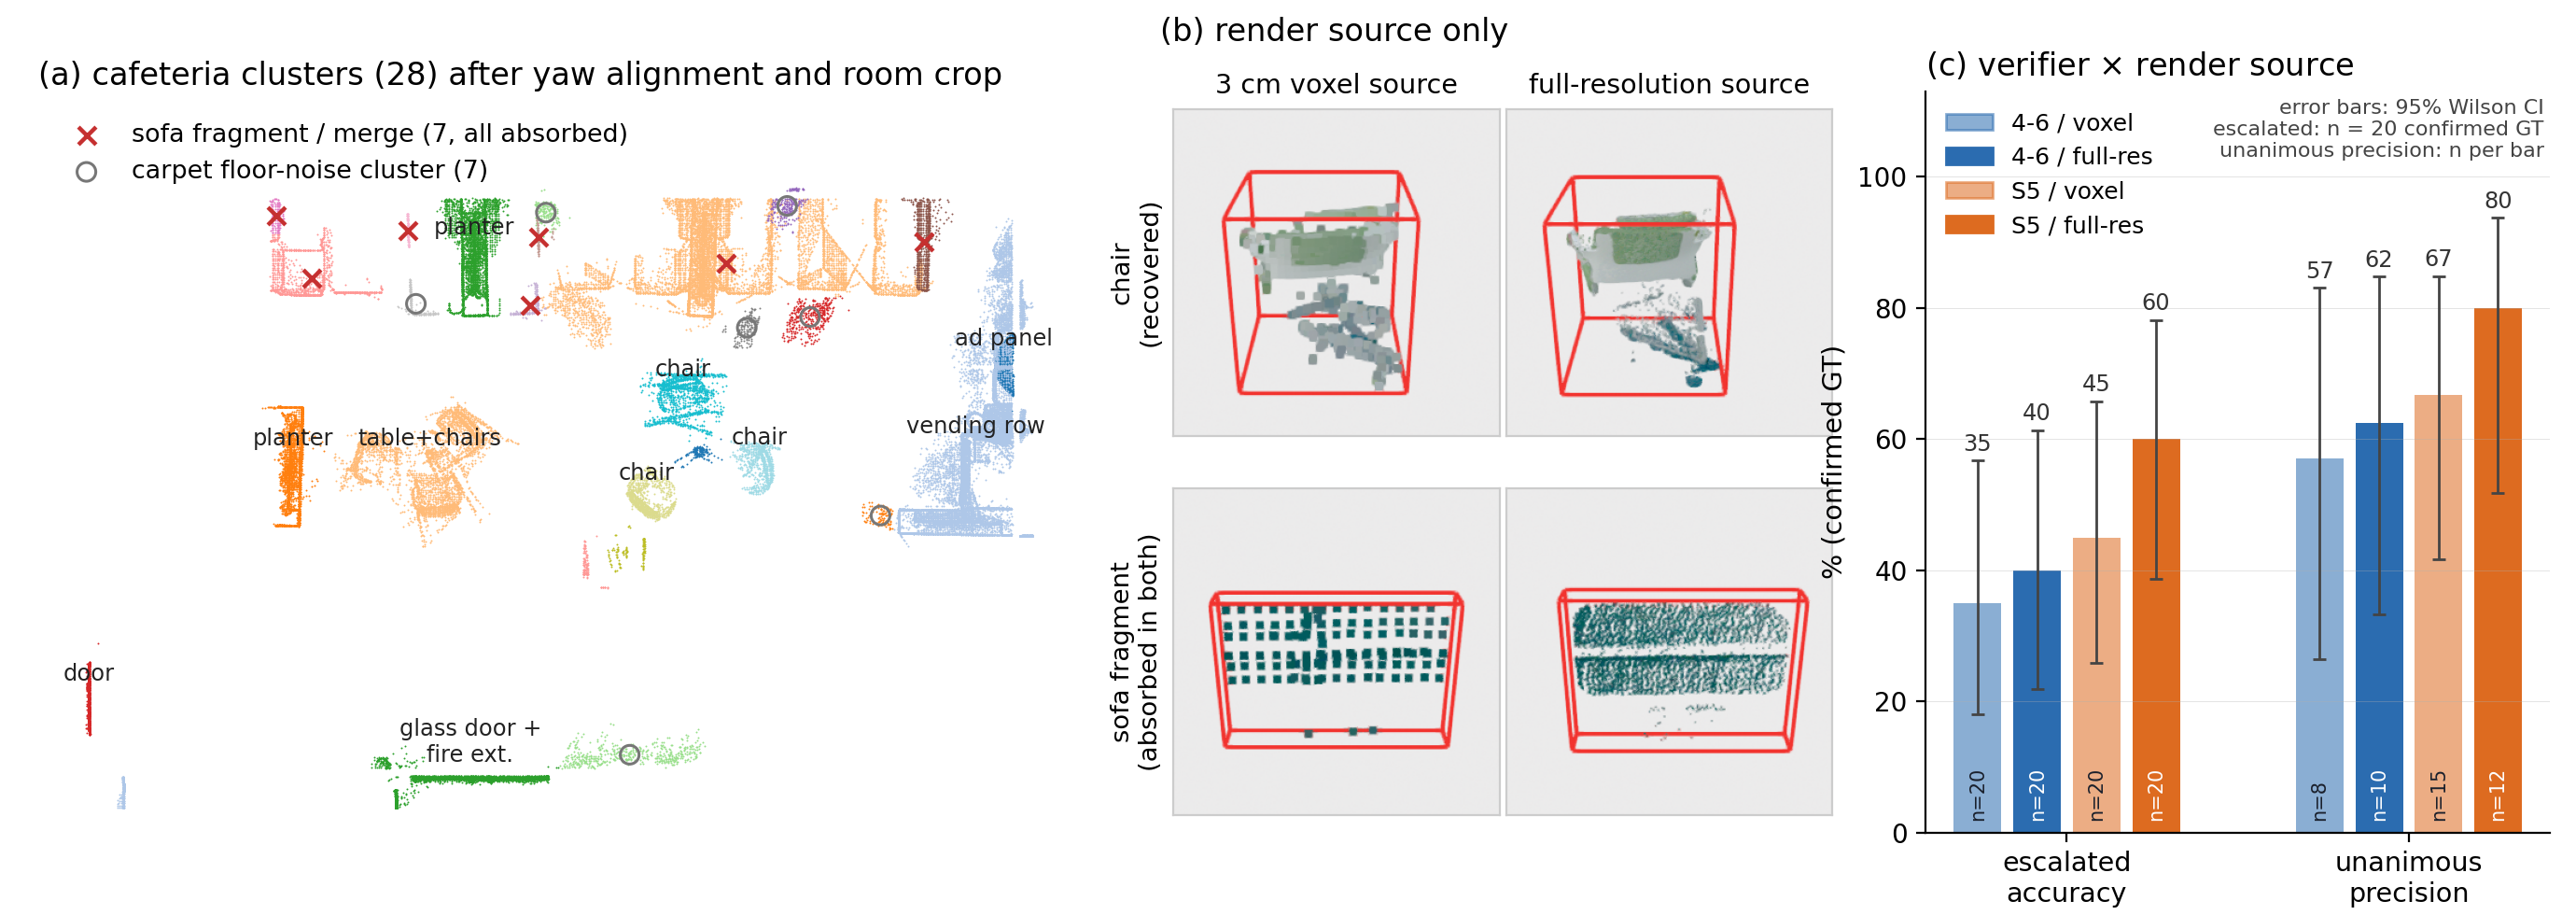
\includegraphics[width=\linewidth]{figures/ele_fig17_cafe_stress.png}
\caption{Cafeteria stress scene. (a)~The 28 clusters after automatic yaw
alignment and room crop; crosses mark the seven sofa fragments/merges,
circles the seven carpet floor-noise clusters. (b)~One cluster rendered from
the 3~cm working cloud (left) and from full-resolution re-associated points
(right): the chair (top) is recovered by the render-source change alone; the
sofa fragment (bottom) is not. (c)~Escalated accuracy and unanimous precision
across verifier $\times$ render source; error bars are 95\% Wilson intervals.}
\label{fig:cafe}
\end{figure}

\paragraph{Cost and latency.}
VLM verification is the only paid stage: full verification averages
$\sim$\$0.09 per object (\$3.63 for a 38-cluster run and \$7.37 for the
86-cluster robot-hall detection set, all calls included), and the incremental
design changes the cost model qualitatively (an identical-input repeat scan
costs \$0). Wall-clock time is equally bounded on the workstation: the full
deterministic backbone---loading the 68.6~M-point E57, 3~cm downsampling,
ten-plane removal, decomposition, and remnant filtering---completes in 29~s
(8.1~GB peak memory), rendering the four-view sets takes 99~s for 88 objects,
and verification with escalation runs in 7.7~min for a 50-object scene at six
concurrent calls, so the complete semantic modeling of a scene finishes in
well under ten minutes end to end. Verification is offline; no VLM call sits
on a robot's control path. Figure~\ref{fig:semmap} visualizes the resulting
semantic map with the confidence gate visible in the map itself.

\begin{figure}[!htb]
\centering
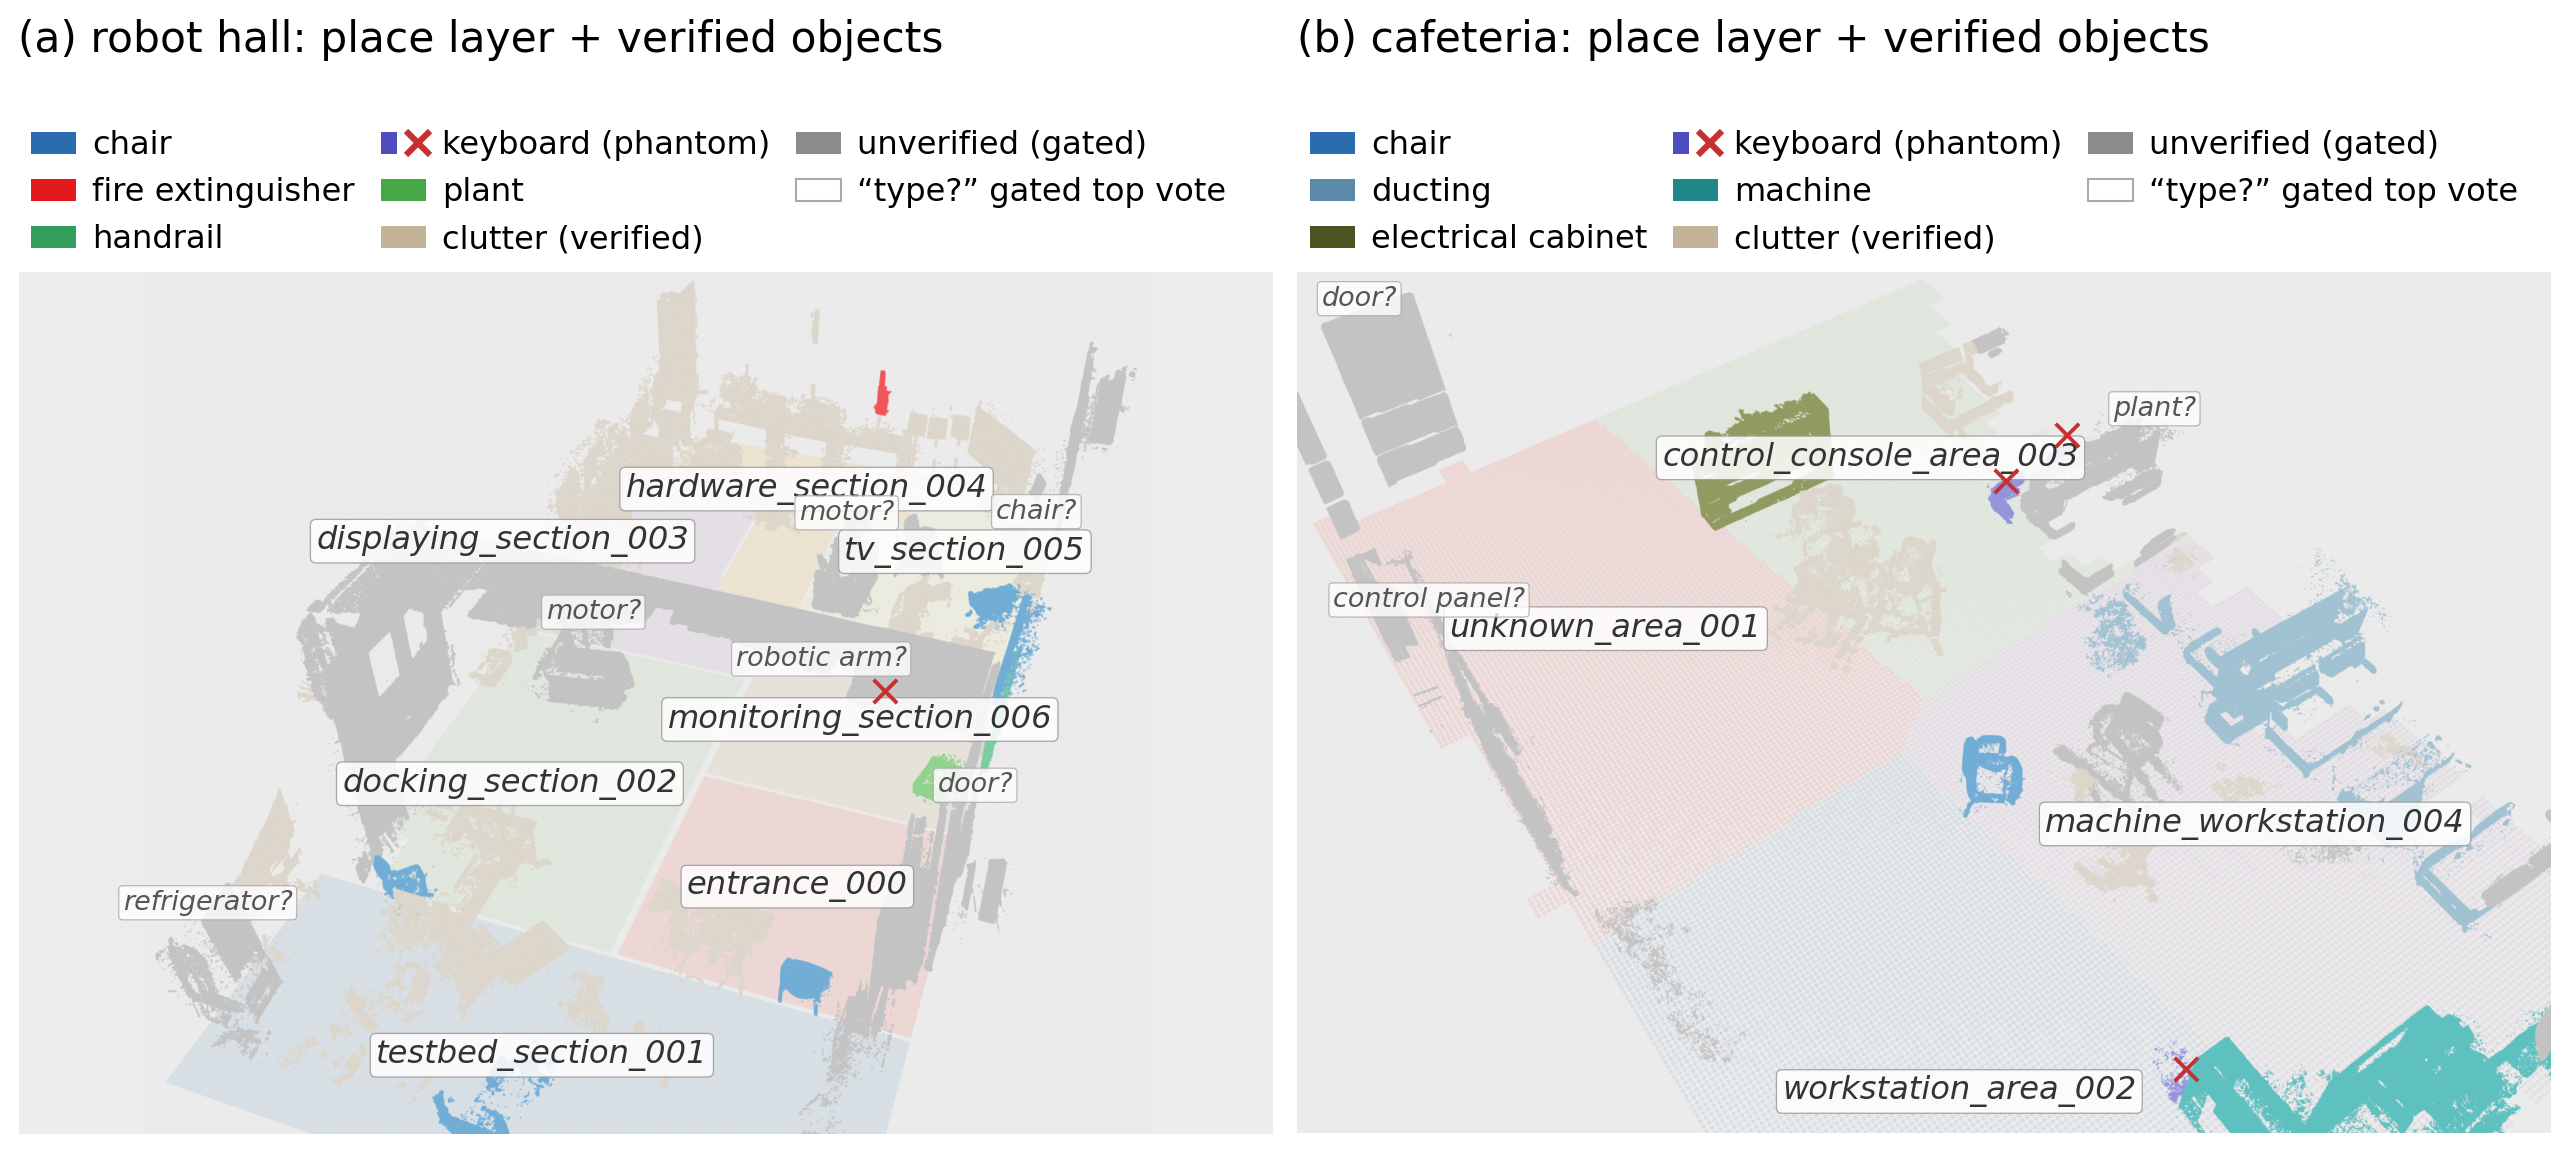
\includegraphics[width=\linewidth]{figures/ele_fig19_semantic_map.png}
\caption{The generated semantic map, visualized at the verification stage
(before owner feedback), so the confidence gate and the errors that pass it
are both visible. (a)~Robot hall: SLIC place-layer regions (pastel floor) with
the room-scoped object clusters rendered as their segmented points, colored by
verified class; gray clusters are \texttt{unverified} and demoted at query
time. (b)~The cafeteria stress scene under the same representation; red
crosses mark verified-keyboard clusters that are owner-refuted phantoms.}
\label{fig:semmap}
\end{figure}

\section{Digital Twin: Conversion, Performance, and Fidelity}
\label{sec:exp-twin}

All twin experiments ran on the desktop workstation of
Section~\ref{subsec:platforms} (Isaac Sim~5.1, ROS~2 Jazzy).

\paragraph{Conversion time and resources.}
Table~\ref{tab:convtime} reports single-run wall-clock times for each pipeline
stage on the 68.5~M-point scan. The complete conversion from raw E57 to a
simulation-ready USD stage takes 78.5~s; the dominant cost is writing the
3.7~M-point visual layer, and a reduced-density variant (485~K points)
completes in 36.5~s. The conversion runs entirely on the CPU, peaking at 8.1~GB
of resident memory with an average utilization of 2.4 cores; the simulator
process occupies 3.1~GB of GPU memory with the full scene and robot
articulation loaded in headless physics-only mode. Authoring a comparable
environment by hand is a multi-day effort, and, unlike manual modeling, the
pipeline can be rerun after every facility change. Every stage is linear in
the number of input points, so conversion time scales roughly linearly with
scan size; the main memory constraint is holding the merged cloud in RAM,
which for facility-scale scans beyond roughly $10^8$ points would call for
chunked streaming of the E57 input.

\begin{table}[htbp]
\centering
\caption{Scan-to-simulation conversion time (68.5~M-point E57). Source:
RAAICON~2026~\cite{raaicon2026}.}
\label{tab:convtime}
\begin{tabular}{l r}
\toprule
\textbf{Stage} & \textbf{Time (s)} \\
\midrule
Floor RANSAC, occupancy grid, ROS map export & 14.8 \\
Dense visual cloud extraction (voxel 0.015~m) & 16.8 \\
Visual layer USD export (3.7~M points) & 46.8 \\
Collision-layer synthesis (1{,}430 boxes) & 0.1 \\
\midrule
\textbf{Total} & \textbf{78.5} \\
\bottomrule
\end{tabular}
\end{table}

\paragraph{Scene complexity and simulation performance.}
The generated stage contains 1{,}430 collision boxes ($\approx$17~K
triangles) and 3{,}725{,}047 rendered points (166~MB USD). With the AMMR
articulation loaded (physics at 120~Hz), headless physics-only simulation
advances at 675 steps/s, a real-time factor of 5.6; with rendering enabled the
simulator sustains 51 rendered frames per second (real-time factor 0.84), and
in the interactive GUI session used for the on-site experiments the viewport
sustained 104 frames per second with the full point layer in view. Before
coupling to the real robot, the swerve base was validated in simulation:
straight-line (1.13~m forward run), lateral (1.45~m strafe), and in-place
rotation ($65^{\circ}$) maneuvers each produced odometry matching the
commanded motion direction, and the flip hysteresis of
Equation~\ref{eq:swerve} eliminated the wheel-speed oscillation otherwise
observed at steering-wrap boundaries.

\paragraph{Live twin verification and simulator-issued goals.}
The bridge contract was verified end to end with the physical AMMR in the
scanned facility (Figure~\ref{fig:pairroom}): the 30~Hz state stream is
received across the Wi-Fi link, the anchor calibration of
Equation~\ref{eq:anchor} converges from a single pose sample, and goals picked
in the simulator drive the real robot through Nav2. During the on-site session
the twin mirrored teleoperated motion continuously across a 3.4~m sweep of the
room. Across two sessions on consecutive days, all four navigation goals
issued by dragging the target marker in the simulator viewport drove the robot
to the corresponding physical locations (Table~\ref{tab:goaltrials},
Figure~\ref{fig:pairgoal}); the twin-frame arrival error of 0.19--0.23~m
(mean 0.21~m) is consistent with the Nav2 goal tolerance, at commanded speeds
up to 0.52~m/s.

\begin{table}[htbp]
\centering
\caption{Simulator-issued navigation-goal trials on the physical AMMR.
Source: RAAICON~2026~\cite{raaicon2026}.}
\label{tab:goaltrials}
\begin{tabular}{c c c l}
\toprule
\textbf{Trial} & \textbf{Session} & \textbf{Error (m)} & \textbf{Note} \\
\midrule
1 & day 1 & 0.19 & 14.4~s run \\
2 & day 1 & 0.21 & \\
3 & day 2 & 0.19 & \\
4 & day 2 & 0.23 & 3.0~m straight, up to 0.52~m/s \\
\midrule
\multicolumn{2}{l}{\textbf{Mean (4/4 reached)}} & \textbf{0.21} & \\
\bottomrule
\end{tabular}
\end{table}

\begin{figure}[!htb]
\centering
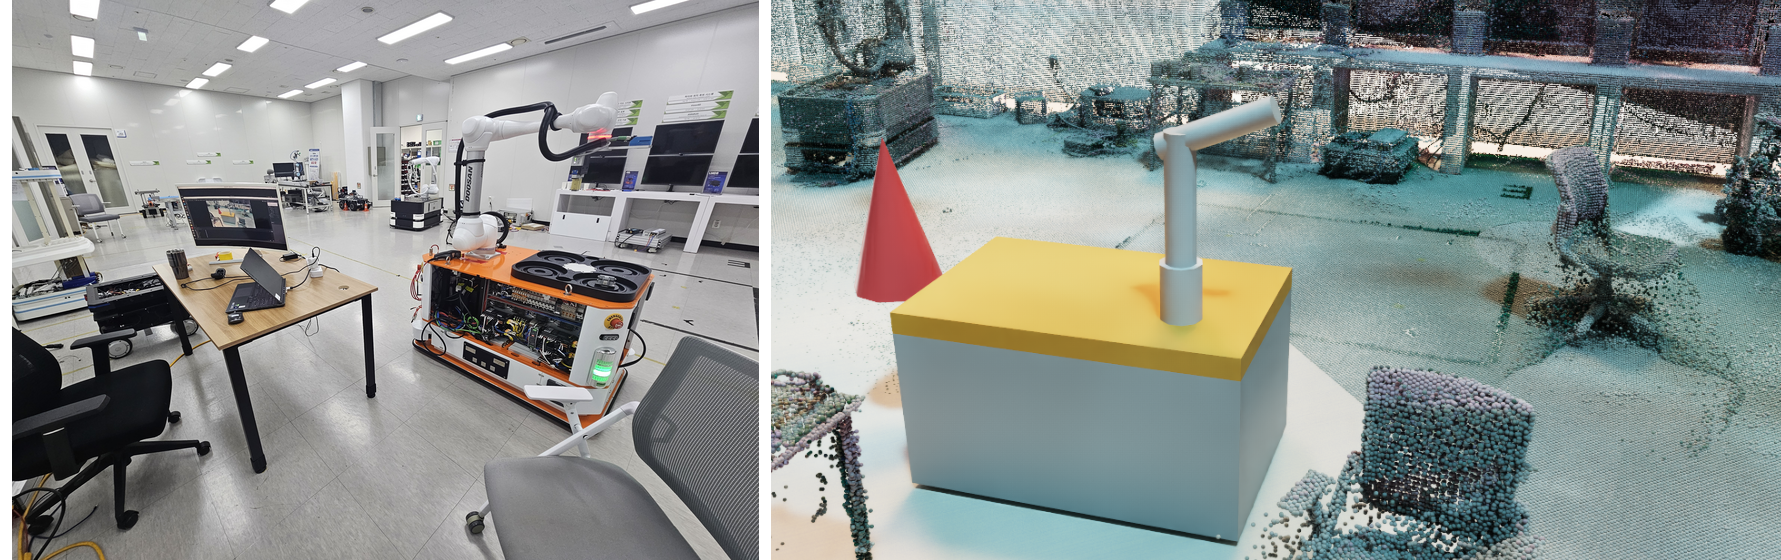
\includegraphics[width=0.95\linewidth]{figures/raa_fig_pair_room.png}
\caption{Test facility (left) and its generated twin during the live session
(right). The yellow body with the white column is the AMMR proxy model; the
red cone is the draggable navigation-goal marker.}
\label{fig:pairroom}
\end{figure}

\begin{figure}[!htb]
\centering
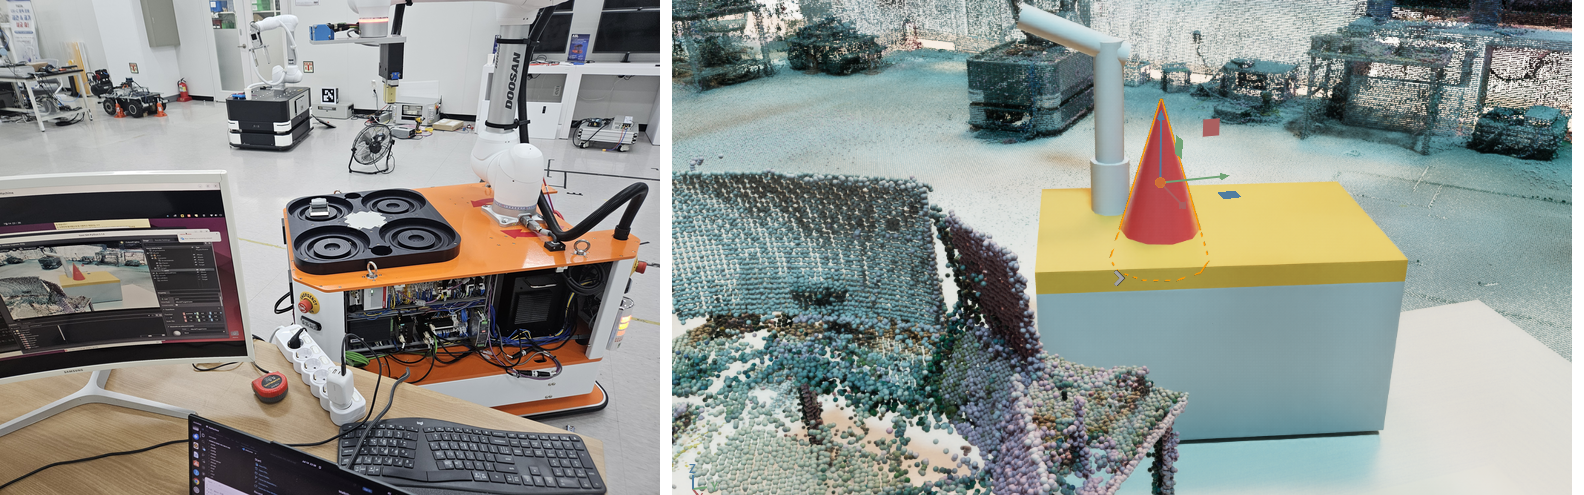
\includegraphics[width=0.95\linewidth]{figures/raa_fig_pair_goal.png}
\caption{Simulator-issued navigation goal. Left: the physical robot at the
reached location; right: the twin after arrival, parked on the goal marker.}
\label{fig:pairgoal}
\end{figure}

\paragraph{Geometric fidelity.}
Metric accuracy is evaluated at two levels. Three room features were
tape-measured and compared against the same dimensions extracted from the
twin's point layer (Table~\ref{tab:geo}): all errors are within 2\% (mean
absolute error 6.4~cm, or 1.3\%), so the scan-to-simulation conversion itself
preserves metric scale to centimeter level. End to end, tape-measured
distances between marked floor checkpoints were compared against the
corresponding distances reported by the twin with the robot parked on each
checkpoint, which captures the full error budget---TLS registration, occupancy
quantization, AMCL localization, and anchor calibration---without requiring a
global frame alignment. Over three checkpoint pairs (0.86, 3.14, and 1.30~m
tape distance) the twin distances deviated by a mean absolute error of 5.5~cm
(RMSE 7.4~cm, maximum 12.5~cm, signed bias $+2.8$~cm; Figure~\ref{fig:eval}).
The largest deviation occurred on the segment executed with large in-place
rotations and matches the AMCL repeatability observed when revisiting the same
floor marker (17~cm), indicating that end-to-end twin accuracy is dominated by
the onboard localization rather than by the reconstructed scene.

\begin{table}[htbp]
\centering
\caption{Scene-feature dimensions: tape measure vs.\ twin point layer.}
\label{tab:geo}
\begin{tabular}{l r r r}
\toprule
\textbf{Feature} & \textbf{Real (m)} & \textbf{Twin (m)} & \textbf{Error} \\
\midrule
Window-side wall length & 8.000 & 7.918 & $-1.0$\% \\
Double-door width & 1.700 & 1.680 & $-1.2$\% \\
Workbench row length & 5.010 & 5.100 & $+1.8$\% \\
\bottomrule
\end{tabular}
\end{table}

\begin{figure}[!htb]
\centering
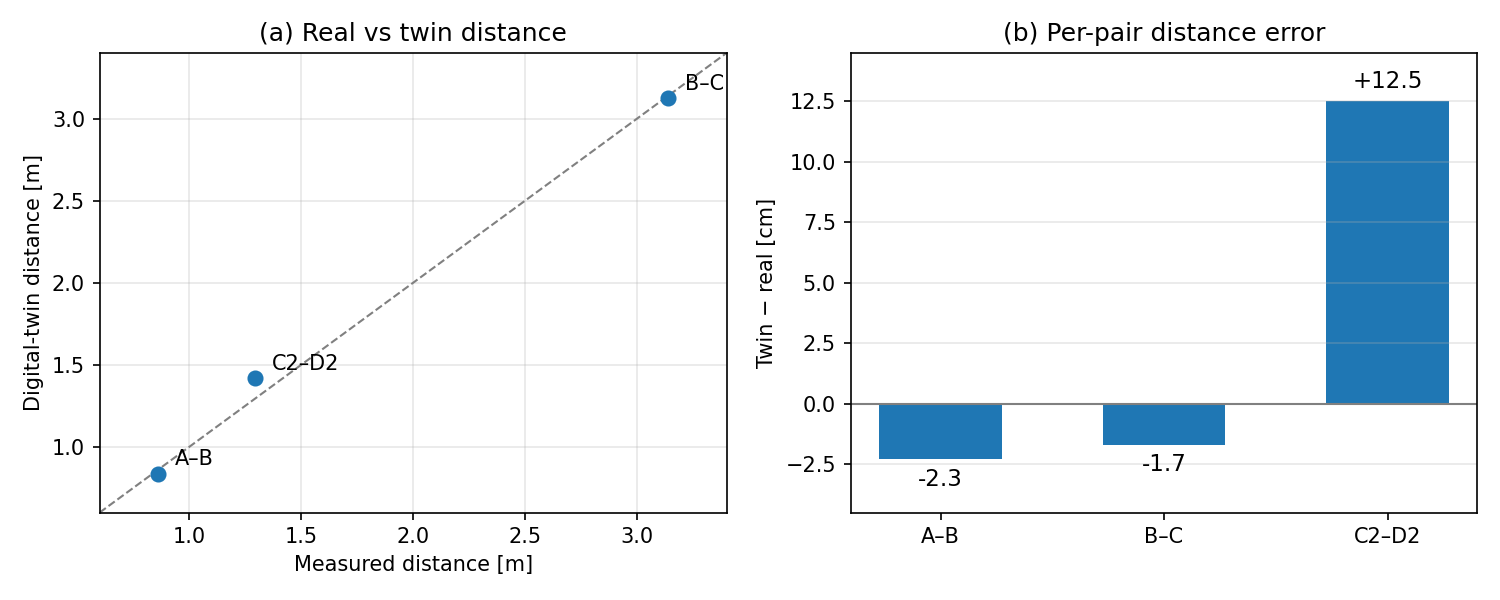
\includegraphics[width=0.95\linewidth]{figures/raa_fig_eval.png}
\caption{Checkpoint-pair distances, tape measure vs.\ twin: scatter against
the identity line (left) and signed per-pair error (right).}
\label{fig:eval}
\end{figure}

\section{Semantic Mission Execution in Simulation and on the Physical Robot}
\label{sec:exp-missions}

\paragraph{Simulation.}
In the Gazebo twin of the test room, over three repetitions of a
three-mission battery (approach the TV, go to the seating area, return home),
task success is 9/9, with mean leg path lengths 4.6/5.4/1.8~m and completion
times 16.5/24.9/15.0~s; semantic resolution latency (command to accepted or
refused goal) is under one second, and a gate refusal stops the robot safely
with zero motion. The reactive layer supplies the safety-stop behavior: a
low-battery event during navigation preempts the active Nav2 goal and returns
the platform to a holding position at home. The phantom experiment
(Table~\ref{tab:semnav}) sends the robot to three owner-refuted phantoms under
two knowledge states. Against the pre-feedback graph, all three phantoms carry
\emph{verified} labels, so the confidence gate passes them---and the waste
takes three distinct forms: a pointless drive to a fluorescent lamp; a
\emph{false arrival} at a 7.4~m ``staircase'' whose approach ring encloses the
robot's own position; and 22~s of futile replanning toward a wall-pillar
``book'' whose approach pose the platform's footprint cannot reach. Against the
graph after structure filtering and owner feedback, the same commands are
refused in about one second with zero motion (Figure~\ref{fig:semnav}).
Verification gating alone cannot stop verified phantoms; it is the combination
of gating, structure-noise removal, and owner feedback that reduces the robot's
exposure to phantom semantic claims.

\begin{table}[htbp]
\caption{Phantom-goal mission waste in simulation (AMMR proxy). The same three
commands are resolved against the knowledge graph before and after structure
filtering + owner feedback (both with the verification gate active).}
\label{tab:semnav}
\centering
\begin{tabular}{l l c c c}
\toprule
\textbf{KG state} & \textbf{Phantom target (truth)} & \textbf{Outcome} & \textbf{Wasted path} & \textbf{Wasted time} \\
\midrule
pre-feedback & keyboard (fluorescent lamp) & driven & 1.7~m & 16.8~s \\
pre-feedback & staircase (bare wall) & false arrival & 0.6~m & 5.7~s \\
pre-feedback & book (wall pillar) & unreachable, aborted & 0~m & 22.2~s \\
\midrule
filtered + owner feedback & all three & refused & 0~m & $\sim$1~s \\
\bottomrule
\end{tabular}
\end{table}

\begin{figure}[!htb]
\centering
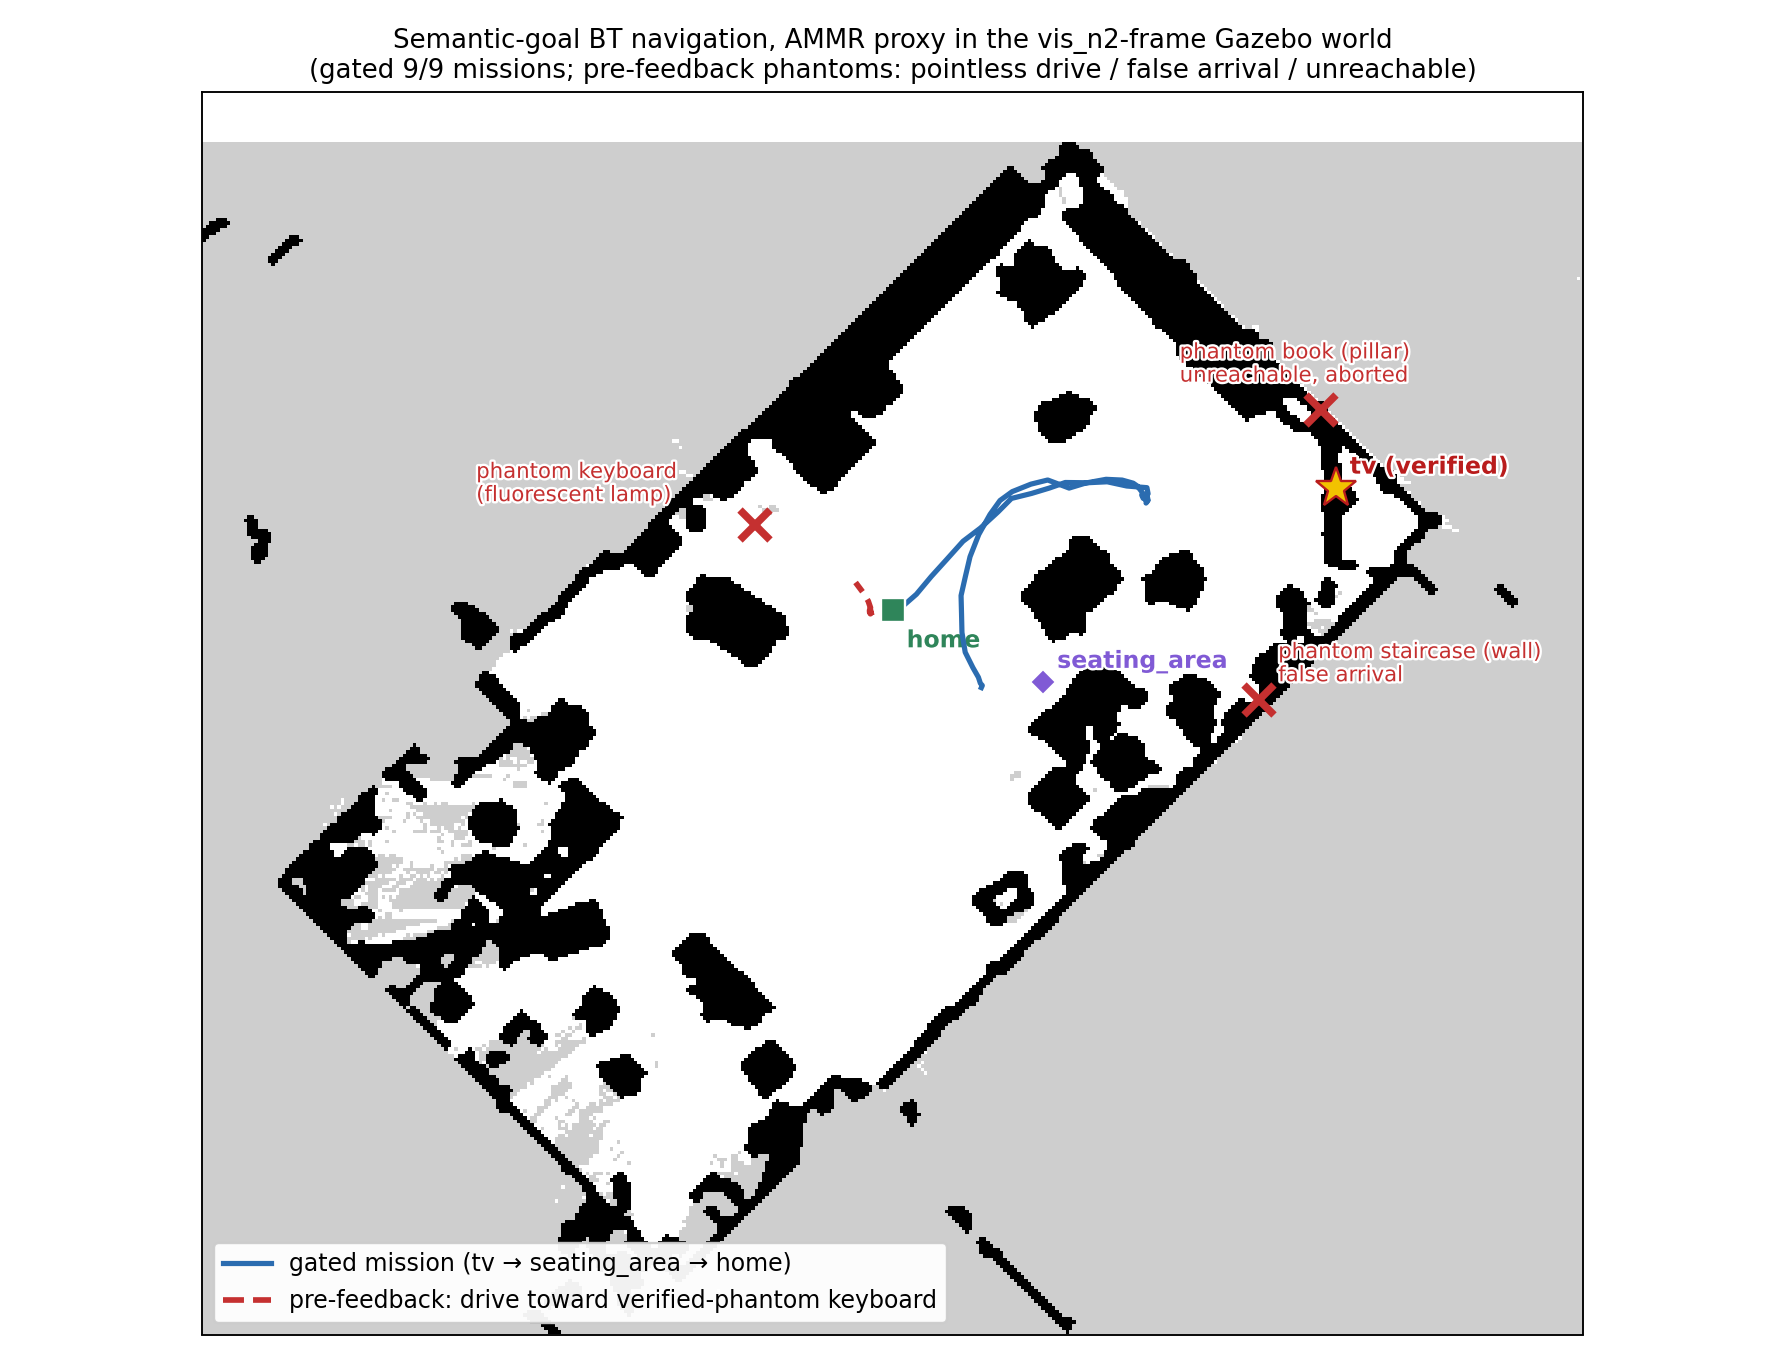
\includegraphics[width=0.8\linewidth]{figures/ele_fig15_semantic_nav_run.png}
\caption{Semantic-goal navigation of the AMMR proxy in the Gazebo twin of the
test room. Blue: a gated three-mission run (TV $\rightarrow$ seating area
$\rightarrow$ home). Red dashed: against the pre-feedback graph the robot
drives toward a verified-phantom keyboard; crosses mark the three phantom goals
with their failure modes. All three are refused once structure filtering and
owner feedback are applied.}
\label{fig:semnav}
\end{figure}

\paragraph{Physical robot.}
The mission stack was run unchanged against the physical AMMR in the test
room (robot-hall configuration) through the bridge of
Section~\ref{sec:real-robot}, with the console, the Isaac Sim twin, and the
robot all served from the same knowledge graph. Three semantic drives
completed---two \texttt{goto\_object} approaches to the wall TV and one
\texttt{goto\_place} drive into the monitor workstation region, each
3.6--4.0~m from the start---in 14--22~s with arrival errors of 0.22--0.34~m
(mean 0.30~m) between the robot's localized pose and the resolved goal; a
place command issued while the robot already stood inside the region completed
without motion (0.11~m from the region goal). The gate behaved as in
simulation: \texttt{goto\_object keyboard}, the owner-refuted phantom of
Table~\ref{tab:semnav}, was refused by the mediator in under one second with
zero robot motion, twice (Table~\ref{tab:realrobot},
Figure~\ref{fig:realrobot}). Missions were issued one at a time from a standing
start. The exercise is a bounded validation---one room, one platform, three
completed drives---but it confirms that the graph that survives verification,
gating, and owner feedback is directly consumable by a real robot, and that the
twin, console, and robot stay consistent because they read one store.

\begin{table}[htbp]
\caption{Real-robot semantic missions on the AMMR (test room, 15 September
2026). Goals are resolved by the mediator in the scan frame; distance is
straight-line start-to-goal; arrival error is the localized-pose-to-goal
distance at mission completion. Source: \emph{Electronics}~\cite{kim2026electronics}.}
\label{tab:realrobot}
\centering
\footnotesize
\begin{tabularx}{\textwidth}{X l c c c X}
\toprule
\textbf{Command} & \textbf{Resolved goal (m)} & \textbf{Dist.} & \textbf{Time} & \textbf{Err.} & \textbf{Outcome} \\
\midrule
\texttt{goto\_object tv} & tv\_006 (3.09, 1.91) & 4.0~m & 14~s & 0.34~m & completed \\
\texttt{goto\_object tv} (Fig.~\ref{fig:realrobot}a) & tv\_006 (3.09, 1.91) & 3.6~m & 20.8~s & 0.33~m & completed \\
\texttt{goto\_place electrical\_ maintenance\_area} (Fig.~\ref{fig:realrobot}b) & region ($-$0.69, 3.81) & 3.9~m & 22.1~s & 0.22~m & completed \\
\texttt{goto\_place display\_ briefing\_area} & region (3.31, 1.76) & 0.1~m & $<$1~s & 0.11~m & completed (already inside) \\
\texttt{goto\_object keyboard} ($\times$2, phantom) & --- & --- & $<$1~s & --- & refused by gate, no motion \\
\bottomrule
\end{tabularx}
\end{table}

\begin{figure}[!htb]
\centering
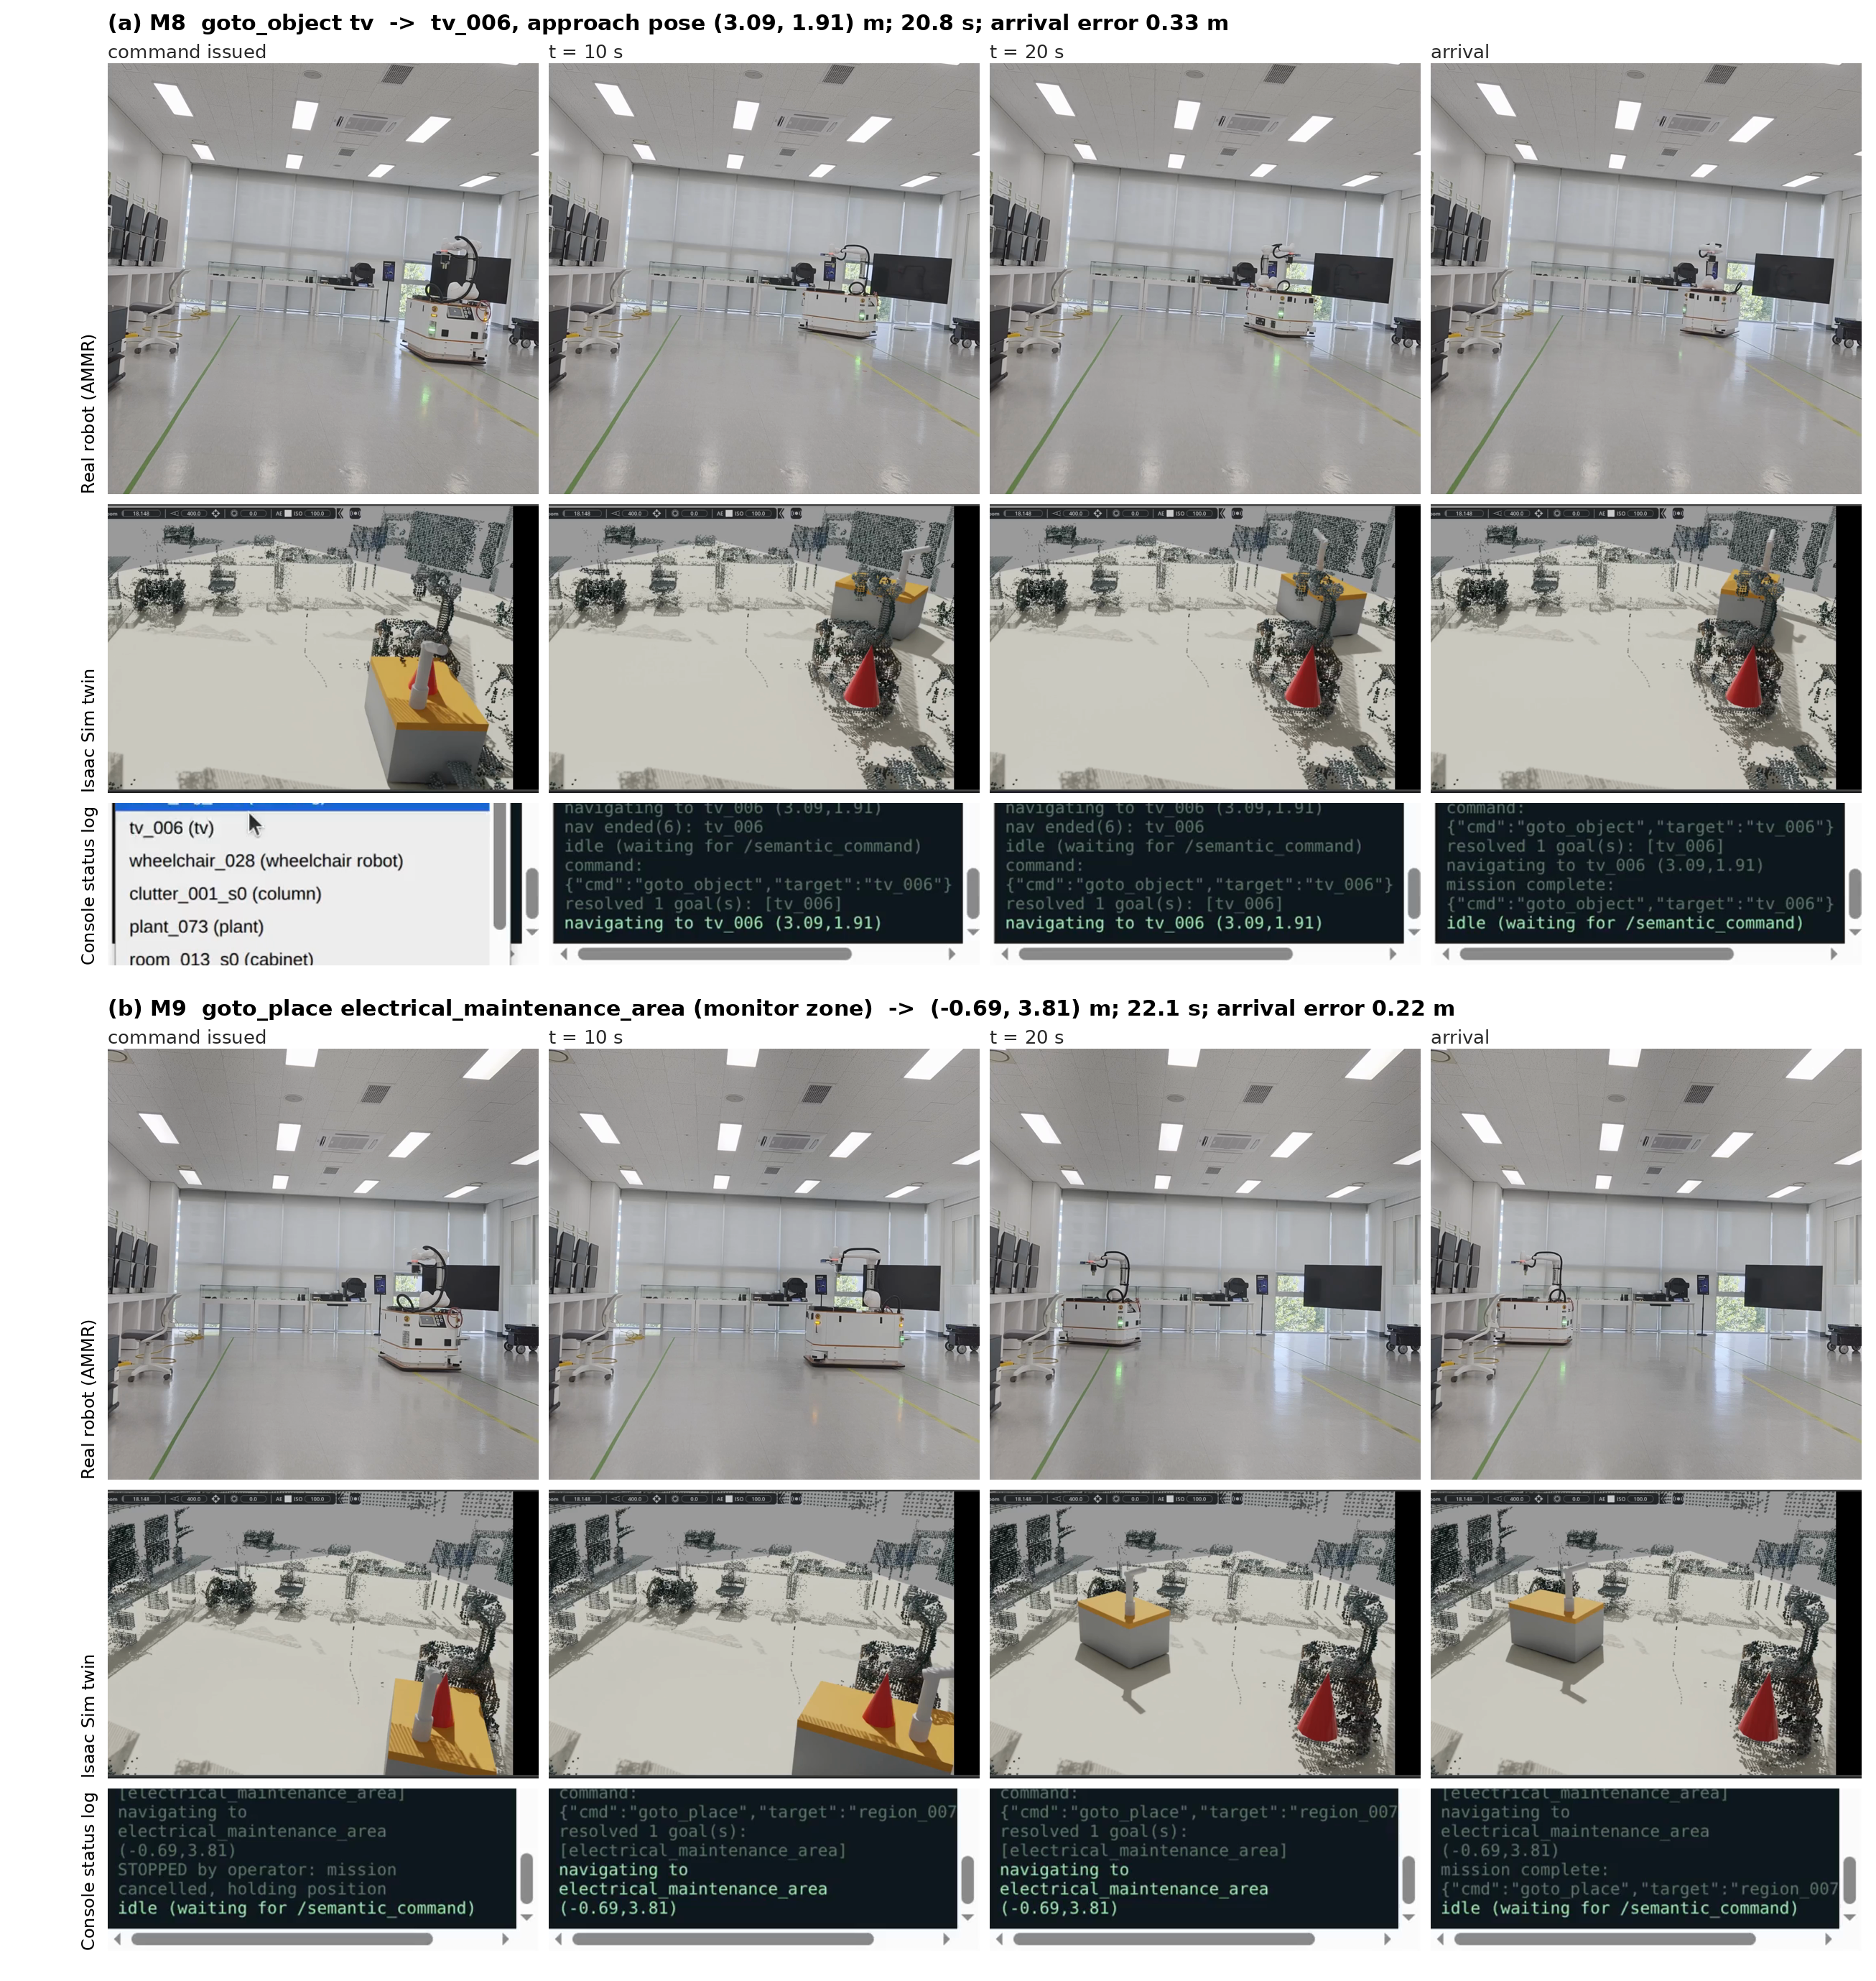
\includegraphics[width=\linewidth]{figures/ele_fig20_real_robot_missions.png}
\caption{Real-robot semantic missions (Table~\ref{tab:realrobot}). Rows: the
physical AMMR, the Isaac Sim twin derived from the same knowledge graph (the
red cone marks the twin's goal handle), and the management console's status
log; columns: command issued, 10~s, 20~s, and arrival. (a)~\texttt{goto\_object
tv}: the mediator resolves the verified node \texttt{tv\_006} to an approach
pose and the robot arrives 0.33~m from it in 20.8~s. (b)~\texttt{goto\_place
electrical\_maintenance\_area}: the region containing the monitor workstation,
reached in 22.1~s with 0.22~m error.}
\label{fig:realrobot}
\end{figure}

\section{Overhead Layer: Ceiling-Mounted Structure}
\label{sec:exp-overhead}

The overhead recognition pass of Section~\ref{sec:overhead} was run with its
parameters frozen on the two industrial epochs (T2, T3) and on the cafeteria
scene. Table~\ref{tab:overhead} summarizes the outcome of each stage and
Figure~\ref{fig:overhead} shows the T3 result over the floor-level graph.

\begin{table}[htbp]
\centering
\caption{Overhead recognition pass on three scenes (parameters frozen; the
verifier and protocol of Section~\ref{sec:exp-verify}). ``Cut'' = clusters
whose bottom lies at the band cut and are dropped as truncated continuations
of floor-level content; in-room = inside the room mask with the 0.5~m wall
tolerance.}
\label{tab:overhead}
\footnotesize\setstretch{1.15}
\begin{tabularx}{\textwidth}{X c c c}
\toprule
 & \textbf{Robot hall (T2)} & \textbf{Re-scan (T3)} & \textbf{Cafeteria} \\
\midrule
Reference cloud (points) & 989~K & 995~K & 546~K \\
Overhead-band points ($>$1.8~m) & 545~K & 512~K & 241~K \\
Ceiling levels found (m above floor) & 3.00 / 3.20 / 3.52 & 3.00 / 3.17 / 3.49 & 3.00 \\
Wall planes & 7 & 6 & 7 \\
Candidate points after ceiling/wall removal & 28.0~K & 39.6~K & 1.4~K \\
Floor-connected candidate points removed & 12.4~K & 31.4~K & 1.2~K \\
Clusters (after cut rule) & 18 & 12 & 0 \\
In-room objects & 5 & 6 & 0 \\
Verified unanimous / escalated / unverified & 1 / 4 / 0 & 1 / 3 / 2 & --- \\
VLM calls / cost & 57 / \$0.55 & 70 / \$0.67 & --- \\
\bottomrule
\end{tabularx}
\end{table}

\begin{figure}[!htb]
\centering
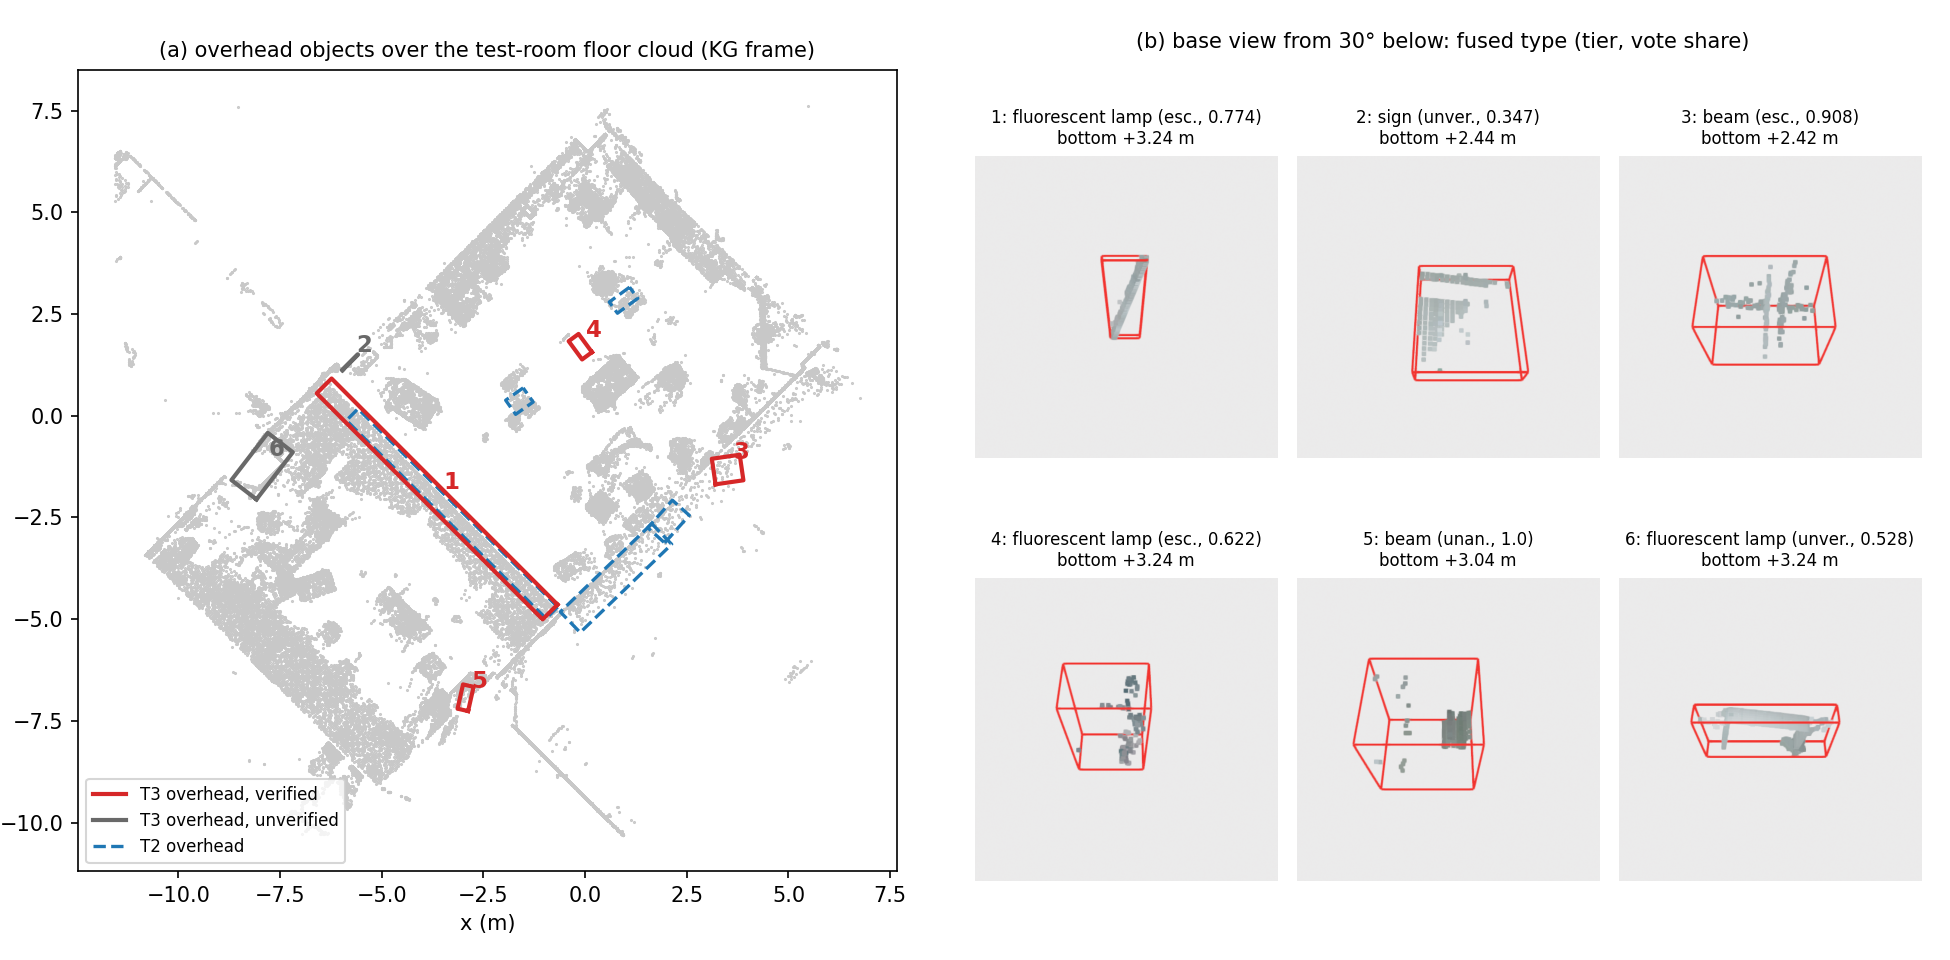
\includegraphics[width=\linewidth]{figures/fig6_overhead.png}
\caption{Overhead layer on the T3 epoch. (a)~The six in-room overhead objects
(red: verified tiers, gray: unverified) over the floor-level cloud, with the
five T2 overhead objects dashed in blue; (b)~each object's base render from
$30^\circ$ below with its fused type, tier, and vote share.}
\label{fig:overhead}
\end{figure}

\paragraph{What the pass finds.}
On T3 the pass isolates six in-room overhead objects: a 7.9~m lighting rail
0.25~m below the top ceiling level (verified as a fluorescent lamp by
escalation), three small fixtures at the same height (one verified
unanimously as a \emph{beam}, one as a fluorescent lamp by escalation, and
one left unverified with \emph{fluorescent lamp} at share 0.53), a hanging
thin plate 2.4~m above the floor (unverified; \emph{sign} at share 0.35),
and a sparse cross-shaped pipe junction (verified as \emph{beam} by
escalation). Every in-room object is attached to a ceiling level
(\emph{ceiling-hung}); the wall-mounted and suspended categories occur only
outside the room. Four of the six are verified (one unanimously, three by
escalation) and two remain unverified, at a cost of under \$1 for the scene.
On T2, the same room scanned from the
robot deck nine days earlier, the pass finds five in-room objects, all
verified (one unanimously, four by escalation). On the cafeteria the pass
finds \emph{nothing}: its single flat ceiling at 3.0~m carries recessed
lights that lie inside the ceiling band, and the 1.4~K candidate points that
survive ceiling and wall removal all belong to floor-connected clusters. A
null result on a scene that has no hanging structure is the intended
behavior of the pass, and it is reported as such.

\paragraph{Ground truth.}
\textcolor{red}{[Owner ground truth for the eleven T3 candidates (union of
the two extraction rules below) is being collected on the sheet
\texttt{overhead\_gt\_sheet.csv}; the precision figures of this paragraph
will be filled in from it.]} A render audit by the author, under the same
protocol as the floor-level audit, grades the lighting rail, the three
fixtures at the top level, the hanging plate, and the pipe junction as
plausible overhead objects; as for the floor pass, render-only annotation
cannot resolve fixture \emph{types} (a lamp housing and a cable tray look
alike from below at 3~cm spacing), so the type precision of the tiers is
reported only against the owner's inventory.

\paragraph{Extraction rule and its alternative.}
The frozen rule decides that a candidate is overhead by connectivity: a
cluster that reaches down into the driving band through the structure-free
lower cloud (at $\varepsilon=0.15$~m) is the upper part of a floor object. An
alternative rule, tested first, excludes candidate points that fall inside
the footprint of a floor-pass object beneath them; on T3 it returned nine
in-room candidates instead of six, because three fixtures that hang within
0.15~m of wall-mounted equipment (a projector-like bracket near the display
wall, a hanging rack, and a boxed unit) are absorbed by the connectivity
test, but on T2 it failed outright: the footprints of that epoch's merged
mega-clusters (Section~\ref{subsec:exp-params}) covered most of the room and
suppressed every fixture. Connectivity is therefore retained as the frozen
rule, and the owner sheet lists the union of both candidate sets so that
the recall cost of the connectivity rule can be scored.

\paragraph{Identity across epochs.}
Overhead objects are the most static content of a room, which makes them a
clean test of the identity policy of Section~\ref{sec:matching}. Upserting
the T2 set and then the T3 set into an overhead graph gives, for the T3
epoch, 0 matched, 1 moved, 5 inserted, and 4 absent. The reason is not
matching but coverage: the two scans see different parts of the ceiling. The
robot-deck exploration scan (T2) resolves the lighting rail and two fixtures
near the room center, whereas the six-setup re-scan (T3) resolves the rail
plus fixtures at the room's ends; only the rail is common to both, and its
centroid shifts by 0.52~m between the epochs because T2 captured 6.9~m of it
and T3 7.9~m---just outside the 0.5~m spatial gate, so the rail is
re-inserted under a new identity (the fragmentation error class of
Section~\ref{sec:exp-update}), and one same-type pair 1.9~m apart is
recorded as a false move. Two conclusions follow. First, ceiling coverage
depends on station placement at least as much as floor coverage does, so
the overhead layer inherits the coverage sensitivity of Part~A. Second,
elongated fixtures need an extent-overlap matching feature rather than a
centroid gate; this is the same feature the floor-level occlusion scenario
of Section~\ref{sec:exp-update} motivated, and it is left to future work.

\paragraph{Consumption.}
Verified overhead objects enter the knowledge graph with
\texttt{heightLevel = high}, their clearance below (2.4--3.2~m in the test
room), and their attachment, and the console and the Isaac Sim twin derive
them from the same store as every other node; a pointing or installation
task resolves against a verified overhead node exactly as a navigation task
resolves against a floor node, with the same gate refusing unverified ones.
No lifting platform executed such a task in this dissertation
(Chapter~\ref{ch:conclusion}).

\section{Summary against the Research Objectives}
\label{sec:exp-summary}

Table~\ref{tab:objsummary} maps the principal results of this chapter back to
the five research objectives of Section~\ref{sec:objectives} and states the
scope of each result.

\begin{table}[htbp]
\centering
\caption{Principal results against the research objectives, with scope.}
\label{tab:objsummary}
\small
\begin{tabularx}{\textwidth}{l X X}
\toprule
\textbf{Obj.} & \textbf{Principal result} & \textbf{Scope} \\
\midrule
O1 & Visibility rule: LOS $77\%\to84$--$85\%$ (paired ablation, $+1$--2 scans); on hardware $77.6\to92.1\%$; all visibility runs register at 4--5~mm bundle error, 84--88\% overlap & Room-scale indoor, 2D visibility, one scanner, one test room \\
O2 & Byte-identical backbone across hosts; recall 0.952 vs.\ owner inventory at the operating point; learned closed-set/projection baselines fail on industrial content & Proxy metrics for baseline screening; one industrial scene \\
O3 & Escalation $77.8\to88.9\%$ / $78.1\to84.4\%$; unanimity 94--100\% precision; gated query 83.3\% with 3/4 traps blocked; zero identity switches over three epochs; re-verification at 3.1\% of rebuild; automated recall $28\to85\%$ & One building; tier precision is scene-scoped (cafeteria 35--60\%); replay on development scene \\
O4 & Scan-to-sim in 78.5~s; RTF 5.6 physics-only, 104~FPS viewport; dimensions within 2\%; end-to-end positioning 5.5~cm MAE; overhead layer: 6 in-room ceiling objects on T3 (5 verified), null result on the flat-ceiling cafeteria & One room; overhead band validated at the representation level, not with a lift \\
O5 & Simulator-issued goals 4/4 (0.21~m); console-issued semantic missions 3 completed (0.30~m mean error), 2 phantom refusals with zero motion; twin, console, robot consistent from one store & One platform (AMMR), missions from a standing start \\
\bottomrule
\end{tabularx}
\end{table}

   % Experiments and Results
%%=============================================================================
%% chapters/conclusion.tex — Conclusion and Future Works (Chapter 7)
%%=============================================================================
\chapter{Conclusion and Future Works}
\label{ch:conclusion}

\section{Conclusion}
\label{sec:conclusion}

This dissertation proposed and validated an integrated framework that
automates 3D mapping and point cloud semantic modeling for spatial-operation
robots. The framework acquires survey-grade 3D point clouds with human
intervention minimized through a stop-and-scan-integrated frontier exploration
strategy whose scan/skip decision is driven by an occlusion-aware visibility
coverage model; transforms the registered clouds into a verified,
confidence-aware, and maintainable TOSM knowledge graph through a deterministic
geometric backbone, multi-view VLM verification with automatic escalation,
identity-preserving incremental update, structurally gated querying, an
object-grounded place layer, and an owner-in-the-loop revision path; derives
from the same model the occupancy, place, and simulation layers that
conventional robot-operation pipelines consume; and supplies the resulting
representation, as a single semantic store, to a digital twin, a management
console, and a physical mobile manipulator.

Three design decisions distinguish the framework from prior work. First, it
makes the coverage model, not the acceptance rule, the decisive component of
stop-and-scan placement: replacing the isotropic disk with a ray-cast
visibility region raised line-of-sight coverage from about 77\% to 84--85\% in
a controlled paired ablation at the cost of one to two scans, and a disk
baseline governed by the identical marginal-gain rule performed markedly worse
in a partitioned world (59.1\% LOS), which attributes the deficiency to the
coverage model itself. On hardware, the visibility rule raised coverage from 77.6\% to
92.1\%, and every visibility run's scans registered offline at survey grade
(4--5~mm bundle error, 84--88\% overlap) whereas disk runs yielded at best a
single-link network and once an unregistrable single scan. Second, it
separates what can be made deterministic from what must remain probabilistic
and controls the probabilistic part with explicit confidence machinery: the
geometric backbone reproduces every cluster byte-identically across hosts,
which makes verification results carryable and diffs meaningful; per-view late
fusion with automatic escalation lifted verification accuracy from 77.8\% to
88.9\% and from 78.1\% to 84.4\% on two configurations of an industrial room
with 94--100\% precision on unanimous votes; structural gating answered 83.3\%
of knowledge-grounded questions while blocking hallucination traps that
instruction-based gating let through; mint-once identities survived three scan
epochs with zero observed identity switches; and selective re-verification
reduced VLM cost to 3.1\% of a rebuild on a controlled re-scan. The study also
surfaced failure modes as valuable as the successes---phantom objects from
ceiling soffits, unanimous-but-wrong verifications, clutter absorption of
site-specific equipment, correlated verifier bias, and a coverage paradox in
which a better scan over-merges density-based clustering---and either fixed
each by a method component (raising automated recall against an owner-audited
inventory from 28\% to 85\%) or reported it as a bounded limitation. Third, it
treats the knowledge graph as the single source of truth for every downstream
consumer: an automated scan-to-simulation pipeline built a physics-enabled
Isaac Sim twin in under 80~s that preserves metric scale to within 2\%, a live
bidirectional bridge mirrored the physical robot at 30~Hz with 5.5~cm mean
end-to-end positioning error, and console-issued semantic missions resolved
against the graph were executed by the physical robot with a mean arrival
error of 0.30~m while owner-refuted phantom goals were refused with zero
motion.

Together these results establish, on one industrial test room observed across
its working life, the end-to-end path from autonomous survey-grade acquisition,
through verified and maintainable semantic modeling, to consumption by a real
spatial-operation robot. The scope is stated plainly: one scanner, one
building with a cross-floor stress scene that bounds domain transfer, one
physical platform, and 2D visibility reasoning. Within that scope, the
evidence supports occlusion-aware visibility rather than Euclidean proximity as
the basis for deciding where a robot should stop and scan, tiered and gated
verification rather than trusted labels as the basis for robot-facing
semantics, and a single revision-tracked store rather than per-consumer exports
as the basis for keeping a twin, a console, and a robot consistent.

\section{Future Works}
\label{sec:future}

The limitations surfaced by the evaluation define the directions for future
work.

\emph{3D visibility and sensor-semantic coverage.} The placement policy
reasons on a 2D occupancy grid, so vertical occlusions are not modeled and
LOS coverage certifies floor-space sight lines rather than full 3D surface
coverage; the deck-mounted scanner's low vantage makes this more consequential
on a robotic platform than in a tripod survey. Extending the coverage model to
a voxel-, octree-, or surface-based 3D visibility representation, refining LOS
into a visibility-weighted coverage that accounts for incidence angle and
range-dependent point density, and attaching a sensor-level semantic
description (penetrating or optical, range, field of view) to the robot model,
so that the same policy adapts across heterogeneous stop-and-scan sensors, are
the principal directions. A downstream navigation validation in which an
independent robot localizes against the completed map to quantify end-use
accuracy is likewise open.

\emph{Overhead layer with a lifting platform.} The overhead recognition
module of Section~\ref{sec:overhead} recovers ceiling-mounted structure from
the same scan and the multilayer representation exposes it as an installation
target, but no lifting platform executed an overhead task in this
dissertation; the mobile manipulator validated the driving band on hardware
and the overhead band at the representation level. Executing a pointing or
installation task against a verified overhead target, and extending the
overhead vocabulary and ground truth beyond one room, are the next steps.

\emph{Vocabulary gaps, small low-reflectance objects, and structure remnants.}
Clutter absorption of site-specific equipment (robots, charging stations) was
the dominant residual error, and injecting site vocabulary naively traded
precision for recall through candidate anchoring. Close-range or re-rendered
imagery, deployment-specific probe sets for per-site tier calibration,
coverage-adaptive decomposition to resolve the mega-cluster paradox, and
extension of the remnant filters to horizontal and sloped ceiling patches and
to carpet floor noise are the next steps. Structural-change updating beyond
the object level, wall- and doorway-aligned place boundaries, and a color-only
perturbation study remain open.

\emph{Multi-site validation and longer campaigns.} Results come from one
scanner and one building; the cafeteria scene shows that the headline
precision figures do not transfer to out-of-vocabulary furnishings without
segmentation- and render-level adaptation. A second facility annotated to the
same owner-audited standard, and a longer multi-mission, multi-robot campaign
on the physical platform, are required before the framework's numbers can be
claimed as general. Along the same line, the real-robot missions were issued
one at a time from a standing start; queued and chained missions, and the
interaction between the mission stack's stop-and-hold behavior and the
platform's own navigation state, warrant a dedicated study.

\emph{Fleet-level consumption of the semantic store.} The single-store design
positions the knowledge graph as the supply layer of a RaaS-oriented task
manager. Extending the TOSM robot layer with live operational state---for
example, load or motor-current profiles reported by the low-level
controller---would let a fleet manager monitor per-region workload on the
same graph and allocate robots across places accordingly; this is a natural
consumer of the representation developed here, though it lies beyond the 3D
modeling focus of this dissertation and is noted as an outlook rather than a
planned extension.
 % Conclusion and Future Works

%%====================== 4. 참고문헌 ==========================================
\bibliographystyle{ieeetr}
\bibliography{references}

%%====================== 5. 국문초록 (논문요약) ===============================
\begin{koreanabstract}
본 학위논문은 측량급 지상 레이저 스캐너(TLS)를 탑재한 이동 로봇이 미지의 실내
환경의 3차원 지도를 자율적으로 획득하고, 정합된 점군을 완전 자동화된 파이프라인을
통해 신뢰도 계층을 갖는 온톨로지 시맨틱 지식 그래프로 변환하며, 동일한 그래프가
디지털 트윈·관제 콘솔·실제 로봇에 공급되는 통합 프레임워크를 제안하고 검증한다.
Part~A는 정지-스캔 통합형 프론티어 탐색으로 획득을 자동화하며, 정지·스캔 결정을
유클리드 근접성이 아니라 실시간 점유격자 위의 폐색 인지 레이캐스트 가시성
커버리지 모델로 내린다. 통제된 쌍대 절제실험에서 가시성 규칙은 시선(LOS)
커버리지를 약 77\%에서 84--85\%로 높였고, Leica BLK360을 탑재한 완전 자율
실기 비교에서는 77.6\%에서 92.1\%로 높였으며 모든 가시성 주행의 스캔이 측량급
(번들 오차 4--5\,mm)으로 정합되었다. Part~B는 결정론적 기하 백본(시드 고정 구조면
제거, 고정 매개변수 분해와 구조 잔재 필터, 명시 모델링)과 다중 시점
비전-언어모델(VLM) 검증(신뢰도 가중 late fusion, 자동 상향 검증), 정체성 보존
증분 갱신, 구조적 게이트 질의, 객체 기반 장소 계층, 소유자 참여 수정 경로로
TOSM 지식 그래프를 구축한다. 상향 검증은 산업용 시험실의 두 구성에서 검증 정확도를
77.8\%→88.9\%, 78.1\%→84.4\%로 높였고 만장일치 투표 정밀도는 94--100\%였으며,
구조적 게이트는 환각 함정을 차단하면서 지식 기반 질의의 83.3\%에 답했고, 통제된
재스캔에서 선택적 재검증은 VLM 비용을 전체 재구축의 3.1\%로 줄였으며, 실제 3
에폭 연구에서 정체성 전환은 관측되지 않았다. Part~C는 표현의 하류 소비를 검증한다.
자동 스캔-시뮬레이션 변환은 80초 이내에 척도 오차 2\% 이내의 물리 기반 NVIDIA
Isaac Sim 트윈을 생성하고, 실시간 양방향 브리지는 실제 이동 매니퓰레이터를 30\,Hz로
미러링하며 종단 간 위치 오차 평균 5.5\,cm를 보였고, 콘솔에서 발행한 시맨틱 임무는
그래프에 대해 해석되어 실제 로봇이 평균 도착 오차 0.30\,m로 수행하였으며 소유자가
반박한 유령 목표는 이동 없이 거부되었다.
\koreankeywords{3D 시맨틱 매핑, 지상 레이저 스캐닝, 정지-스캔 탐색, 가시성
커버리지, 비전-언어모델 검증, 삼중항 온톨로지 시맨틱 모델, 지식 그래프, 디지털 트윈}
\end{koreanabstract}

%%====================== 6. 측면표지(책등) ===========================
\makesidecover

\end{document}
